\documentclass[a4paper,12pt,oneside,onecolumn]{article} % Document type

\usepackage[left=1.0in, right=1.0in, top=1.0in, bottom=1.0in]{geometry}

\usepackage{fontspec}
\setmainfont{cmr12}
\usepackage{amsmath,amssymb}
\usepackage{xltxtra}
\defaultfontfeatures{Ligatures=TeX}
\usepackage[english]{babel}
\usepackage[square,numbers]{natbib}
\bibliographystyle{plainnat}
\usepackage{float}
\usepackage{pgfplots}
\usepackage{tikz}
\usepackage{lscape}
\usepackage{graphicx}
\usepackage{pstricks}
\usepackage{subfigure}
\usepackage{multicol}
\usepackage{caption}
\usepackage{rotating}
\usepackage{lastpage}
\usepackage{fancyhdr}
\usepackage{caption}
\usepackage{titling}
\usepackage{pdflscape}
\usepackage{tabularx}
\usepackage[hidelinks]{hyperref}
\usepackage{url}
\pagestyle{fancy}
\lhead{Slip Control}
\rhead{EL2425}
\chead{Final Report}
\rfoot{Page \thepage\ of \pageref{LastPage}}
\cfoot{}
\renewcommand{\footrulewidth}{0.4pt}


\pretitle{%
  \begin{center}
  \LARGE
  
\includegraphics[scale=0.3]{./images/KTH_Logotyp_RGB_2013.eps}\\[\bigskipamount]
}
\posttitle{\end{center}}

\title{
	\vspace{1in}
  EL$2425\ -$ Automatic Control, Project Course \\
  \vspace{0.2in}
  Slip Control
}
%\date{}

\begin{document}

	\maketitle

  \vfill

  \begin{center}

    \large Final report
    \vfill
    Alexandros Filotheou, Melih Guldogus, Tengfan Lin,\\ Roberto Sanchez-Rey, Xuechun Xu
  \end{center}

  \newpage
  \tableofcontents
  \newpage

\section{Introduction}

  The kinematic model is tested by a series of specific control signal. By pushing the control signal into the estimation model and comparing the output with the car behavior published by Mocap, the kinematic model can be verified. The result is shown in the figure \ref{fig:mesh1}.

\begin{figure}[h]
    \centering
    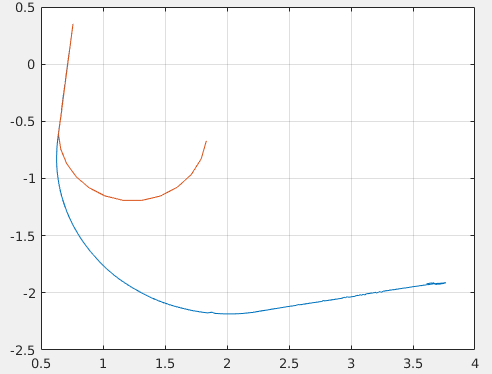
\includegraphics[width=0.85\textwidth]{./figures/kmver}
    \caption{Model and car behavior under a series of specific control signal}
    \label{fig:mesh1}
\end{figure}

As can be seen in the figure \ref{fig:mesh1}, red curve represents the model behavior while the blue one is the real car. The most probably reason that the deviation exists is that the car slips when turing.


\subsection{Dynamic model equations}

\begin{align*}
    & x_g(k+1) = x_g(k) + T_s (v_x(k) \cos(\psi(k)) - v_y(k) \sin(\psi(k)) \\
    & y_g(k+1) = y_g(k) + T_s (v_x(k) \sin(\psi(k)) + v_y(k) \cos(\psi(k)) \\
    & \psi(k+1) = \psi(k) + T_s r(k)\\
    & v_x(k+1) = v_x(k) + T_s / m C_f (\arctan((v_y(k)+r(k) l_f)/v_x(k)) - \delta(k)) \sin(\delta(k)) + T_s r(k) v_y(k)\\
    & v_y(k+1) = v_y(k) - T_s / m C_r \arctan((v_y(k)-r(k) l_r)/v_x(k)) - \\
    & \hspace{19mm}T_s C_f / m (\arctan((v_y(k)+r(k) l_f)/v_x(k))-\delta(k)) \cos(\delta(k)) - T_s r(k) v_x(k)\\
    & r(k+1) = r(k) - T_s l_f C_f/J_z \cos(\delta(k)) (\arctan((v_y(k)+r(k) l_f)/v_x(k))-\delta(k)) +\\
    & \hspace{19mm}T_s C_r / J_z \arctan((v_y(k)-r(k) l_r)/v_x(k))\\
    & v(k+1) = v(k) + T_s (v_ref(k) - \sqrt{v_x(k)^2 + v_y(k)^2})/\tau
\end{align*}

The $v_x,v_y$ are the velocity component at local coordinate, while $x_g, y_g$ are the position component at global coordinate.\\
There are three parameters in the model need to be defined i.e.  inertia of the car around z-direction $J_z$, cornering stiffness for front and rear wheels $C_f, C_r$. The estimation of these will be described next.

\subsection{Parameter estimation}

Here we use similar method to the one used in time-constant estimation. By putting certain series of input signals, both velocity and steering angle, the Mocap system generate the corresponding position signals as car running. Meanwhile in Matlab we generate the estimated position signals with the dynamic model given the same series of input.
The next step is to use Matlab
Will do it with Matlab function \texttt{Simulink Design Optimization} toolbox to find the optimize solutions of the problem in
\begin{equation}
  \min_{J_z, C_f, C_r} estimate\_error = (measurement - estimate\_position)^2
\end{equation}
The aim is to generate a qualified dynamic model which will be used as the inner model of the MPC controller, in order to drive the car as fast as possible. But due to the time limitation, we have not manage to achieve some satisfying parameters.
\end{document}


\section{Documentation resources}

  The kinematic model is tested by a series of specific control signal. By pushing the control signal into the estimation model and comparing the output with the car behavior published by Mocap, the kinematic model can be verified. The result is shown in the figure \ref{fig:mesh1}.

\begin{figure}[h]
    \centering
    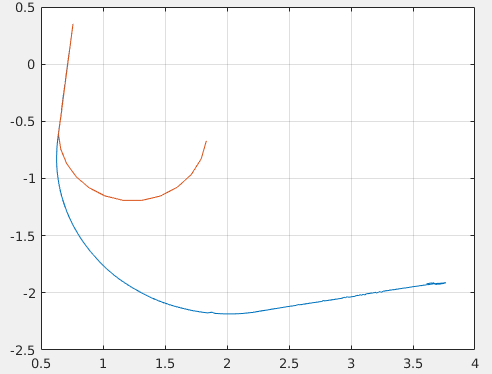
\includegraphics[width=0.85\textwidth]{./figures/kmver}
    \caption{Model and car behavior under a series of specific control signal}
    \label{fig:mesh1}
\end{figure}

As can be seen in the figure \ref{fig:mesh1}, red curve represents the model behavior while the blue one is the real car. The most probably reason that the deviation exists is that the car slips when turing.


\subsection{Dynamic model equations}

\begin{align*}
    & x_g(k+1) = x_g(k) + T_s (v_x(k) \cos(\psi(k)) - v_y(k) \sin(\psi(k)) \\
    & y_g(k+1) = y_g(k) + T_s (v_x(k) \sin(\psi(k)) + v_y(k) \cos(\psi(k)) \\
    & \psi(k+1) = \psi(k) + T_s r(k)\\
    & v_x(k+1) = v_x(k) + T_s / m C_f (\arctan((v_y(k)+r(k) l_f)/v_x(k)) - \delta(k)) \sin(\delta(k)) + T_s r(k) v_y(k)\\
    & v_y(k+1) = v_y(k) - T_s / m C_r \arctan((v_y(k)-r(k) l_r)/v_x(k)) - \\
    & \hspace{19mm}T_s C_f / m (\arctan((v_y(k)+r(k) l_f)/v_x(k))-\delta(k)) \cos(\delta(k)) - T_s r(k) v_x(k)\\
    & r(k+1) = r(k) - T_s l_f C_f/J_z \cos(\delta(k)) (\arctan((v_y(k)+r(k) l_f)/v_x(k))-\delta(k)) +\\
    & \hspace{19mm}T_s C_r / J_z \arctan((v_y(k)-r(k) l_r)/v_x(k))\\
    & v(k+1) = v(k) + T_s (v_ref(k) - \sqrt{v_x(k)^2 + v_y(k)^2})/\tau
\end{align*}

The $v_x,v_y$ are the velocity component at local coordinate, while $x_g, y_g$ are the position component at global coordinate.\\
There are three parameters in the model need to be defined i.e.  inertia of the car around z-direction $J_z$, cornering stiffness for front and rear wheels $C_f, C_r$. The estimation of these will be described next.

\subsection{Parameter estimation}

Here we use similar method to the one used in time-constant estimation. By putting certain series of input signals, both velocity and steering angle, the Mocap system generate the corresponding position signals as car running. Meanwhile in Matlab we generate the estimated position signals with the dynamic model given the same series of input.
The next step is to use Matlab
Will do it with Matlab function \texttt{Simulink Design Optimization} toolbox to find the optimize solutions of the problem in
\begin{equation}
  \min_{J_z, C_f, C_r} estimate\_error = (measurement - estimate\_position)^2
\end{equation}
The aim is to generate a qualified dynamic model which will be used as the inner model of the MPC controller, in order to drive the car as fast as possible. But due to the time limitation, we have not manage to achieve some satisfying parameters.
\end{document}


  \newpage

  \section{Tracking the centerline of a lane using a PID controller}

    \subsection{Theoretical approach to solution}
      In figure \ref{fig:circular_mpc}, the vehicle $C$, whose velocity is constant
and denoted by $v$, is to track a circle whose center is $O'$ and whose
radius is $R$. Its orientation relative to the global coordinate system is
$\psi$. The vehicle's coordinates are $(x_c, y_c)$. The circular trajectory
is known a priori, and is comprised of a set of ordered points who encode
the $x$-wise, $y$-wise and $yaw$-wise states that the vehicle ought to have,
that is, each point on the circle serves as a reference to the vehicle. In terms
of yaw angle, the longitudinal axis of the vehicle ought to always be tangent
to the circle.


\begin{figure}[H]\centering
  \scalebox{0.7}{In figure \ref{fig:circular_mpc}, the vehicle $C$, whose velocity is constant
and denoted by $v$, is to track a circle whose center is $O'$ and whose
radius is $O'R$. Its orientation relative to the global coordinate system is
$\psi$. $R$ is the point $C$ is to track. The orientation of $R$ relative to
the global coordinate system is $\theta$. The vehicle's coordinates are
$(x_c, y_c)$. The aim is to find the vehicle's deviation from $R$ in terms of
translation along the $x$ and $y$ axes and rotation around the $x$-axis.

\begin{figure}[H]\centering
  \scalebox{0.8}{In figure \ref{fig:circular_mpc}, the vehicle $C$, whose velocity is constant
and denoted by $v$, is to track a circle whose center is $O'$ and whose
radius is $O'R$. Its orientation relative to the global coordinate system is
$\psi$. $R$ is the point $C$ is to track. The orientation of $R$ relative to
the global coordinate system is $\theta$. The vehicle's coordinates are
$(x_c, y_c)$. The aim is to find the vehicle's deviation from $R$ in terms of
translation along the $x$ and $y$ axes and rotation around the $x$-axis.

\begin{figure}[H]\centering
  \scalebox{0.8}{\input{./figures/circular_mpc.tex}}
  \caption{}
  \label{fig:circular_mpc}
\end{figure}

The solution to the problem can be decomposed into two separate components:
a translational and a rotational one.

\subsubsection{Translational component}

Here, we assume that the orientation of the tangent at $R$ is the same of that
of the vehicle and equal to $\psi$. Given the distance $RC$ (the coordinates of
both $R$ and $C$ are known) we are interested in finding the displacements
$RC_x$ and $RC_y$. From triangle $C_yRC$ we can immediately deduce that

\begin{align}
  RC_x &= RC sin\psi \\
  RC_y &= -RC cos\psi \\
\end{align}

where $RC = \sqrt{(x_C - x_R)^2 + (y_C - y_R)^2}$

\begin{figure}[H]\centering
  \scalebox{0.8}{\input{./figures/circular_mpc_translational.tex}}
  \caption{}
  \label{}
\end{figure}


\subsubsection{Rotational component}

Here, we assume that the only deviation of $C$ from $R$ is only in terms of
orientation. From figure \ref{fig:circular_mp_rotational} we can easily
discern that the angular error is $\theta -\psi$.

\begin{figure}[H]\centering
  \scalebox{0.8}{\input{./figures/circular_mpc_rotational.tex}}
  \caption{}
  \label{fig:circular_mp_rotational}
\end{figure}


\subsubsection{Obtaining the relevant linearized kinematic model}

The model constitutes the equations of motion of the vehicle, and has three
states ($x$, $y$ and $\psi$) and one input ($\delta$). The equations of the
vehicle's motion that are relevant here are

\begin{align}
  \dot{x} &= v cos(\psi + \beta) \\
  \dot{y} &= v sin(\psi + \beta) \\
  \dot{\psi} &= \dfrac{v}{l_r} sin\beta
\end{align}

Sampling with a sampling time of $T_s$ gives

\begin{align}
  x_{k+1} &= x_{k} + T_s v cos(\psi_k + \beta_k) \\
  y_{k+1} &= y_{k} + T_s v sin(\psi_k + \beta_k) \\
  \psi_{k+1} &= \psi_{k} + T_s \dfrac{v}{l_r} sin\beta_k
\end{align}

where

\begin{align}
  \beta_k = tan^{-1}\Big(\dfrac{l_r}{l_r + l_f} tan\delta_k\Big)
\end{align}


Forming the Jacobians for matrices $A$, $B$ and evaluating them at time
$t=k$ around $\delta = 0$ (which makes $\beta = 0$) gives

\begin{equation}
 A =
  \begin{bmatrix}
    1 & 0 & -T_s v sin(\psi_k + \beta_k) \\\\
    0 & 1 & T_s v cos(\psi_k + \beta_k) \\\\
    0 & 0 & 1
  \end{bmatrix}
  =
  \begin{bmatrix}
    1 & 0 & -T_s v sin\Big(\psi_k + tan^{-1} (l_q tan\delta_k)\Big) \\\\
    0 & 1 & T_s v cos\Big(\psi_k + tan^{-1} (l_q tan\delta_k)\Big) \\\\
    0 & 0 & 1
  \end{bmatrix}
\end{equation}
\begin{equation}
 A =
  \begin{bmatrix}
    1 & 0 & -T_s v sin(\psi_k) \\\\
    0 & 1 & T_s v cos(\psi_k) \\\\
    0 & 0 & 1
  \end{bmatrix}
\end{equation}

\begin{equation}
 B =
  \begin{bmatrix}
    -T_s v sin(\psi_k + \beta_k) \dfrac{l_q}{l_q^2 sin^2\delta_k + cos^2\delta_k} \\
    T_s v cos(\psi_k + \beta_k) \dfrac{l_q}{l_q^2 sin^2\delta_k + cos^2\delta_k} \\
    \dfrac{T_s v}{l_r} cos(\beta_k) \dfrac{l_q}{l_q^2 sin^2\delta_k + cos^2\delta_k}
  \end{bmatrix}
  =
  \begin{bmatrix}
    -T_s v sin\Big(\psi_k + tan^{-1} (l_q tan\delta_k)\Big) \dfrac{l_q}{l_q^2 sin^2\delta_k + cos^2\delta_k} \\
    T_s v cos\Big(\psi_k + tan^{-1} (l_q tan\delta_k)\Big) \dfrac{l_q}{l_q^2 sin^2\delta_k + cos^2\delta_k} \\
    \dfrac{T_s v}{l_r} cos\Bigg(tan^{-1} \Big(l_q tan\delta_k\Big)\Bigg) \dfrac{l_q}{l_q^2 sin^2\delta_k + cos^2\delta_k}
  \end{bmatrix}
\end{equation}
\begin{equation}
 B =
  \begin{bmatrix}
    -\dfrac{T_s l_r v}{l_r + l_f} sin\psi_k \\\\
    \dfrac{T_s l_r v}{l_r + l_f} cos\psi_k \\\\
    \dfrac{T_s v}{l_r+l_f}
  \end{bmatrix}
\end{equation}

where $l_q = \dfrac{l_r}{l_r + l_f}$




Now we can express the linear model as

\begin{align}
  s_{k+1} = A s_k + B \delta_k
\end{align}

where

\begin{equation}
  s=
  \begin{bmatrix}
    x_{k} \\
    y_{k} \\
    \psi_{k}
  \end{bmatrix}
\end{equation}

or

\begin{equation}
  \begin{bmatrix}
    x_{k+1} \\
    y_{k+1} \\
    \psi_{k+1}
  \end{bmatrix}
  =
  \begin{bmatrix}
    1 & 0 & -T_s v sin(\psi_k) \\\\
    0 & 1 & T_s v cos(\psi_k) \\\\
    0 & 0 & 1
  \end{bmatrix}
  \begin{bmatrix}
    x_{k} \\
    y_{k} \\
    \psi_{k}
  \end{bmatrix}
  +
  \begin{bmatrix}
    -\dfrac{T_s l_r v}{l_r + l_f} sin\psi_k \\\\
    \dfrac{T_s l_r v}{l_r + l_f} cos\psi_k \\\\
    \dfrac{T_s v}{l_r+l_f}
  \end{bmatrix}
  \delta_{k}
\end{equation}



\subsubsection{Stating the optimization problem}

We can now form the optimization problem as

\begin{align}
  \text{minimize }    & \sum\limits_{k=0}^N x_k^2 q_x + y_k^2 q_y + \phi_k^2 q_{\phi} + \delta_k^2 r \\
  \text{subject to }  & s_{k+1} = A s_k + B \delta_k,\text{ where } s_k = [x_k, y_k, \phi_k]^T \\
                      & \delta_{min} \leq \delta_k \leq \delta_{max} \\
                      & x_0 = RC sin\phi_0 \\
                      & y_0 = -RC cos\phi_0 \\
                      & \phi_0 = \theta_R - \psi
\end{align}
}
  \caption{}
  \label{fig:circular_mpc}
\end{figure}

The solution to the problem can be decomposed into two separate components:
a translational and a rotational one.

\subsubsection{Translational component}

Here, we assume that the orientation of the tangent at $R$ is the same of that
of the vehicle and equal to $\psi$. Given the distance $RC$ (the coordinates of
both $R$ and $C$ are known) we are interested in finding the displacements
$RC_x$ and $RC_y$. From triangle $C_yRC$ we can immediately deduce that

\begin{align}
  RC_x &= RC sin\psi \\
  RC_y &= -RC cos\psi \\
\end{align}

where $RC = \sqrt{(x_C - x_R)^2 + (y_C - y_R)^2}$

\begin{figure}[H]\centering
  \scalebox{0.8}{% Generated with LaTeXDraw 2.0.8
% Fri Nov 18 15:10:06 CET 2016
% \usepackage[usenames,dvipsnames]{pstricks}
% \usepackage{epsfig}
% \usepackage{pst-grad} % For gradients
% \usepackage{pst-plot} % For axes
\scalebox{1} % Change this value to rescale the drawing.
{
\begin{pspicture}(0,-7.3264065)(23.47,7.306406)
\pscircle[linewidth=0.04,dimen=outer](8.36,0.61640626){4.63}
\psline[linewidth=0.04cm,arrowsize=0.05291667cm 2.0,arrowlength=1.4,arrowinset=0.4]{<-}(0.97,7.286406)(0.97,-6.5135937)
\psline[linewidth=0.04cm,arrowsize=0.05291667cm 2.0,arrowlength=1.4,arrowinset=0.4]{->}(0.97,-6.5135937)(23.45,-6.5135937)
\psline[linewidth=0.04cm,arrowsize=0.05291667cm 2.0,arrowlength=1.4,arrowinset=0.4]{->}(15.11,-3.0335937)(18.47,2.1264062)
\psdots[dotsize=0.12](15.11,-3.0535936)
\usefont{T1}{ptm}{m}{n}
\rput(0.27453125,6.6764064){$y$}
\usefont{T1}{ptm}{m}{n}
\rput(22.734531,-7.123594){$x$}
\psdots[dotsize=0.12](8.36,0.61640626)
\psline[linewidth=0.02cm](8.35,0.6064063)(15.11,-3.0535936)
\usefont{T1}{ptm}{m}{n}
\rput(0.58453125,-7.043594){$O$}
\usefont{T1}{ptm}{m}{n}
\rput(14.994532,-3.8235939){$C$}
\usefont{T1}{ptm}{m}{n}
\rput(7.6045313,0.03640625){$O'$}
\psline[linewidth=0.02cm](9.57,-6.5135937)(15.37,3.4864063)
\psline[linewidth=0.02cm,arrowsize=0.05291667cm 2.0,arrowlength=1.4,arrowinset=0.4]{->}(12.39,-5.193594)(12.39,4.726406)
\psline[linewidth=0.02cm,arrowsize=0.05291667cm 2.0,arrowlength=1.4,arrowinset=0.4]{->}(10.19,-1.5735937)(19.53,-1.5935937)
\psline[linewidth=0.02cm,linestyle=dashed,dash=0.16cm 0.16cm](12.39,-3.0535936)(15.05,-3.0535936)
\psline[linewidth=0.02cm,linestyle=dashed,dash=0.16cm 0.16cm](15.11,-3.0535936)(15.11,-1.5735937)
\usefont{T1}{ptm}{m}{n}
\rput(11.694531,-1.8435937){$R$}
\usefont{T1}{ptm}{m}{n}
\rput(11.994532,-3.3235939){$C_y$}
\usefont{T1}{ptm}{m}{n}
\rput(15.094531,-1.2235937){$C_x$}
\psarc[linewidth=0.02](16.43,-1.4135938){0.24}{315.0}{113.62938}
\usefont{T1}{ptm}{m}{n}
\rput(17.244532,-1.2635938){$\psi$}
\usefont{T1}{ptm}{m}{n}
\rput(13.004531,-2.4635937){$\psi$}
\psarc[linewidth=0.02](12.6,-1.9635937){0.25}{218.6598}{42.27369}
\psarc[linewidth=0.02](12.77,-1.4135938){0.24}{315.0}{113.62938}
\usefont{T1}{ptm}{m}{n}
\rput(13.584531,-1.2635938){$\psi$}
\psline[linewidth=0.02cm](12.39,-1.0935937)(11.87,-1.0935937)
\psline[linewidth=0.02cm](11.85,-1.0935937)(11.85,-1.5735937)
\psdots[dotsize=0.12](12.11,-1.3335937)
\end{pspicture} 
}

}
  \caption{}
  \label{}
\end{figure}


\subsubsection{Rotational component}

Here, we assume that the only deviation of $C$ from $R$ is only in terms of
orientation. From figure \ref{fig:circular_mp_rotational} we can easily
discern that the angular error is $\theta -\psi$.

\begin{figure}[H]\centering
  \scalebox{0.8}{% Generated with LaTeXDraw 2.0.8
% Fri Nov 18 16:47:11 CET 2016
% \usepackage[usenames,dvipsnames]{pstricks}
% \usepackage{epsfig}
% \usepackage{pst-grad} % For gradients
% \usepackage{pst-plot} % For axes
\scalebox{1} % Change this value to rescale the drawing.
{
\begin{pspicture}(0,-7.3264065)(23.597345,7.306406)
\pscircle[linewidth=0.04,dimen=outer](8.487344,0.6164076){4.63}
\psline[linewidth=0.04cm,arrowsize=0.05291667cm 2.0,arrowlength=1.4,arrowinset=0.4]{<-}(1.0973437,7.286406)(1.0973437,-6.5135937)
\psline[linewidth=0.04cm,arrowsize=0.05291667cm 2.0,arrowlength=1.4,arrowinset=0.4]{->}(1.0973437,-6.5135937)(23.577345,-6.5135937)
\psline[linewidth=0.04cm,arrowsize=0.05291667cm 2.0,arrowlength=1.4,arrowinset=0.4]{->}(12.530937,-1.6135932)(15.837343,0.94640744)
\usefont{T1}{ptm}{m}{n}
\rput(0.27453125,6.6764073){$y$}
\usefont{T1}{ptm}{m}{n}
\rput(22.734531,-7.123594){$x$}
\psdots[dotsize=0.12](8.487344,0.6164076)
\psline[linewidth=0.02cm](8.4773445,0.6064075)(12.5364065,-1.613593)
\usefont{T1}{ptm}{m}{n}
\rput(0.58453125,-7.043594){$O$}
\usefont{T1}{ptm}{m}{n}
\rput(8.004531,0.0164075){$O'$}
\psline[linewidth=0.02cm,linestyle=dashed,dash=0.17638889cm 0.10583334cm](6.1373444,-6.5135937)(12.96,-1.2735938)
\psarc[linewidth=0.02](7.1018753,-6.213594){0.38}{310.9144}{99.09028}
\usefont{T1}{ptm}{m}{n}
\rput(8.034531,-5.943594){$\psi$}
\psline[linewidth=0.02cm](9.801874,-6.5135937)(13.541874,0.24640727)
\psline[linewidth=0.02cm](12.601875,-1.4535928)(16.341875,5.306406)
\psarc[linewidth=0.02](10.241876,-6.213594){0.38}{310.9144}{99.09028}
\usefont{T1}{ptm}{m}{n}
\rput(11.514531,-5.9235926){$\theta$}
\usefont{T1}{ptm}{m}{n}
\rput(10.764531,-1.6435927){$R \equiv C$}
\usefont{T1}{ptm}{m}{n}
\rput(14.304531,0.45640698){$\theta - \psi$}
\psarc[linewidth=0.02](13.546407,-0.443593){0.35}{340.46335}{130.76361}
\psline[linewidth=0.04cm](11.976405,-1.293593)(12.236406,-0.7735928)
\psline[linewidth=0.04cm](12.256407,-0.79359293)(12.756407,-1.073593)
\psdots[dotsize=0.12](12.376407,-1.213593)
\end{pspicture} 
}

}
  \caption{}
  \label{fig:circular_mp_rotational}
\end{figure}


\subsubsection{Obtaining the relevant linearized kinematic model}

The model constitutes the equations of motion of the vehicle, and has three
states ($x$, $y$ and $\psi$) and one input ($\delta$). The equations of the
vehicle's motion that are relevant here are

\begin{align}
  \dot{x} &= v cos(\psi + \beta) \\
  \dot{y} &= v sin(\psi + \beta) \\
  \dot{\psi} &= \dfrac{v}{l_r} sin\beta
\end{align}

Sampling with a sampling time of $T_s$ gives

\begin{align}
  x_{k+1} &= x_{k} + T_s v cos(\psi_k + \beta_k) \\
  y_{k+1} &= y_{k} + T_s v sin(\psi_k + \beta_k) \\
  \psi_{k+1} &= \psi_{k} + T_s \dfrac{v}{l_r} sin\beta_k
\end{align}

where

\begin{align}
  \beta_k = tan^{-1}\Big(\dfrac{l_r}{l_r + l_f} tan\delta_k\Big)
\end{align}


Forming the Jacobians for matrices $A$, $B$ and evaluating them at time
$t=k$ around $\delta = 0$ (which makes $\beta = 0$) gives

\begin{equation}
 A =
  \begin{bmatrix}
    1 & 0 & -T_s v sin(\psi_k + \beta_k) \\\\
    0 & 1 & T_s v cos(\psi_k + \beta_k) \\\\
    0 & 0 & 1
  \end{bmatrix}
  =
  \begin{bmatrix}
    1 & 0 & -T_s v sin\Big(\psi_k + tan^{-1} (l_q tan\delta_k)\Big) \\\\
    0 & 1 & T_s v cos\Big(\psi_k + tan^{-1} (l_q tan\delta_k)\Big) \\\\
    0 & 0 & 1
  \end{bmatrix}
\end{equation}
\begin{equation}
 A =
  \begin{bmatrix}
    1 & 0 & -T_s v sin(\psi_k) \\\\
    0 & 1 & T_s v cos(\psi_k) \\\\
    0 & 0 & 1
  \end{bmatrix}
\end{equation}

\begin{equation}
 B =
  \begin{bmatrix}
    -T_s v sin(\psi_k + \beta_k) \dfrac{l_q}{l_q^2 sin^2\delta_k + cos^2\delta_k} \\
    T_s v cos(\psi_k + \beta_k) \dfrac{l_q}{l_q^2 sin^2\delta_k + cos^2\delta_k} \\
    \dfrac{T_s v}{l_r} cos(\beta_k) \dfrac{l_q}{l_q^2 sin^2\delta_k + cos^2\delta_k}
  \end{bmatrix}
  =
  \begin{bmatrix}
    -T_s v sin\Big(\psi_k + tan^{-1} (l_q tan\delta_k)\Big) \dfrac{l_q}{l_q^2 sin^2\delta_k + cos^2\delta_k} \\
    T_s v cos\Big(\psi_k + tan^{-1} (l_q tan\delta_k)\Big) \dfrac{l_q}{l_q^2 sin^2\delta_k + cos^2\delta_k} \\
    \dfrac{T_s v}{l_r} cos\Bigg(tan^{-1} \Big(l_q tan\delta_k\Big)\Bigg) \dfrac{l_q}{l_q^2 sin^2\delta_k + cos^2\delta_k}
  \end{bmatrix}
\end{equation}
\begin{equation}
 B =
  \begin{bmatrix}
    -\dfrac{T_s l_r v}{l_r + l_f} sin\psi_k \\\\
    \dfrac{T_s l_r v}{l_r + l_f} cos\psi_k \\\\
    \dfrac{T_s v}{l_r+l_f}
  \end{bmatrix}
\end{equation}

where $l_q = \dfrac{l_r}{l_r + l_f}$




Now we can express the linear model as

\begin{align}
  s_{k+1} = A s_k + B \delta_k
\end{align}

where

\begin{equation}
  s=
  \begin{bmatrix}
    x_{k} \\
    y_{k} \\
    \psi_{k}
  \end{bmatrix}
\end{equation}

or

\begin{equation}
  \begin{bmatrix}
    x_{k+1} \\
    y_{k+1} \\
    \psi_{k+1}
  \end{bmatrix}
  =
  \begin{bmatrix}
    1 & 0 & -T_s v sin(\psi_k) \\\\
    0 & 1 & T_s v cos(\psi_k) \\\\
    0 & 0 & 1
  \end{bmatrix}
  \begin{bmatrix}
    x_{k} \\
    y_{k} \\
    \psi_{k}
  \end{bmatrix}
  +
  \begin{bmatrix}
    -\dfrac{T_s l_r v}{l_r + l_f} sin\psi_k \\\\
    \dfrac{T_s l_r v}{l_r + l_f} cos\psi_k \\\\
    \dfrac{T_s v}{l_r+l_f}
  \end{bmatrix}
  \delta_{k}
\end{equation}



\subsubsection{Stating the optimization problem}

We can now form the optimization problem as

\begin{align}
  \text{minimize }    & \sum\limits_{k=0}^N x_k^2 q_x + y_k^2 q_y + \phi_k^2 q_{\phi} + \delta_k^2 r \\
  \text{subject to }  & s_{k+1} = A s_k + B \delta_k,\text{ where } s_k = [x_k, y_k, \phi_k]^T \\
                      & \delta_{min} \leq \delta_k \leq \delta_{max} \\
                      & x_0 = RC sin\phi_0 \\
                      & y_0 = -RC cos\phi_0 \\
                      & \phi_0 = \theta_R - \psi
\end{align}
}
  \caption{}
  \label{fig:circular_mpc}
\end{figure}

In this setting, since an optimization problem will have to be solved at each
time instant $t$, the first thing that needs to be identified is the reference
pose of the vehicle at each time instant $t$. More precisely, since the
objective is the minimization of the deviation of the vehicle's trajectory
from the circular one, and the framework is that of MPC, we need to identify
the sequence of points on the circle that shall act as references while
iterating through the prediction equations of the linearized model of the
vehicle's behaviour. This task is divided into two sub-tasks: first, we
identify the point $T$ of the circle that lies on the line that is tangent to
the circle and that passes through the position of the vehicle. When this
point is known, the sequence of $N-1$ reference poses can be calculated,
given knowledge of the circle's radius and the vehicle's velocity. $N$ is the
horizon length. The following two sections illustrate the procedures by
which the $N$ reference poses are identified.

\subsubsection{Finding $T$}

Here, we are not concerned with the orientation of the vehicle; its coordinates
will only be used as a point to identify the tangent that passes through
the position of the vehicle.


\begin{figure}[H]\centering
  \scalebox{0.8}{% Generated with LaTeXDraw 2.0.8
% Mon Dec 05 00:44:20 CET 2016
% \usepackage[usenames,dvipsnames]{pstricks}
% \usepackage{epsfig}
% \usepackage{pst-grad} % For gradients
% \usepackage{pst-plot} % For axes
\scalebox{1} % Change this value to rescale the drawing.
{
\begin{pspicture}(0,-7.3264065)(23.597345,7.306406)
\pscircle[linewidth=0.04,dimen=outer](8.487344,0.6164076){4.63}
\psline[linewidth=0.04cm,arrowsize=0.05291667cm 2.0,arrowlength=1.4,arrowinset=0.4]{<-}(1.0973437,7.286406)(1.0973437,-6.5135937)
\psline[linewidth=0.04cm,arrowsize=0.05291667cm 2.0,arrowlength=1.4,arrowinset=0.4]{->}(1.0973437,-6.5135937)(23.577345,-6.5135937)
\usefont{T1}{ptm}{m}{n}
\rput(0.27453125,6.6764073){$y$}
\usefont{T1}{ptm}{m}{n}
\rput(22.734531,-7.123594){$x$}
\psdots[dotsize=0.12](8.487344,0.6164076)
\usefont{T1}{ptm}{m}{n}
\rput(0.58453125,-7.043594){$O$}
\usefont{T1}{ptm}{m}{n}
\rput(7.6045313,0.0364075){$O'$}
\psdots[dotsize=0.12](15.6,3.8064063)
\usefont{T1}{ptm}{m}{n}
\rput(16.424532,3.8964062){$C$}
\psline[linewidth=0.02cm](15.58,3.8064063)(3.36,6.5064063)
\psline[linewidth=0.02cm](8.48,0.6064063)(9.52,5.106406)
\psline[linewidth=0.02cm](8.5,0.62640625)(15.6,3.7864063)
\psarc[linewidth=0.02](14.5,3.6264062){0.42}{104.03625}{249.14554}
\usefont{T1}{ptm}{m}{n}
\rput(13.644531,3.6564062){$\alpha$}
\usefont{T1}{ptm}{m}{n}
\rput(9.834531,5.7964063){$T$}
\psline[linewidth=0.02cm](10.08,5.0264063)(9.94,4.4264064)
\psline[linewidth=0.02cm](9.94,4.4264064)(9.38,4.5664062)
\psdots[dotsize=0.06](9.72,4.746406)
\psline[linewidth=0.02cm,linestyle=dashed,dash=0.16cm 0.16cm](8.48,0.64640623)(18.2,0.64640623)
\psarc[linewidth=0.02](9.68,0.82640624){0.52}{341.56506}{54.29331}
\usefont{T1}{ptm}{m}{n}
\rput(10.824532,1.0164063){$\beta$}
\usefont{T1}{ptm}{m}{n}
\rput(8.344531,2.7564063){$R$}
\end{pspicture} 
}

}
  \caption{}
  \label{fig:circular_mpc_tan}
\end{figure}


In triangle $TO'C$, $\angle O'TC$ is right, and

\begin{align}
  \alpha = sin^{-1} \dfrac{R}{O'C}
\end{align}

while

\begin{align}
  \beta = tan^{-1} \dfrac{y_c - y_{O'}}{x_c - x_{O'}}
\end{align}

Point $T$ is then rudimentary to find: it is the point that lies on the
circle and is found while rotating by $\beta + \dfrac{\pi}{2} - \alpha$ from the
$x$ axis. The coordinates of point $T$ are

\begin{align}
  x_T &= x_{O'} + R cos\theta_T \\
  y_T &= y_{O'} + R sin\theta_T \\
  \theta_T &= \beta + \dfrac{\pi}{2} - \alpha \\
\end{align}

The same reasoning applies to when the vehicle is located at every other
quadrant. The pose that the vehicle ought to have at point $T$ of the circle
can now be retrieved from the given set of poses. Point $T$ shall serve as the
first reference for the vehicle in the statement of the optimization problem,
that is, $s_T = [x_T, y_T, \psi_T]^T = s_0^{ref}$. The next task is now to
find the next $N-1$ reference poses in the circle that the vehicle ought to
refer to.

\subsubsection{Beyond point $T$}

The next reference points depend on the velocity of the vehicle. Since its
velocity is constant, we know from elementary physics that $v = \omega R$,
which means that $\omega = v / R$, which is known, since the radius of the
circle is set by us in advance, and the velocity of the vehicle is measurable.
If we denote with $\theta_T$ the angle that the line passing through $O'$
and $T$ makes with the $x$ axis, with $\theta_1$ the angle that the line
passing through $O'$ and the first reference point after point $T$ makes with
the $x$ axis, and $T_s$ the sampling time of the pose of the vehicle, then

\begin{align}
  \omega &= \dfrac{\Delta \theta}{\Delta t} = \dfrac{\theta_1 - \theta_T}{T_s} \Leftrightarrow \\
  \theta_1 &= \theta_T + T_s \dfrac{v}{R} \\
\end{align}

In general, the $k$-th point in the sequence of the $N-1$ reference points will
lie at an angle of

\begin{align}
  \theta_k &= \theta_T + k T_s \dfrac{v}{R}\\
\end{align}

The coordinates of the $k$-th reference point ($1 \leq k \leq N-1$) are

\begin{align}
  x_k^{ref} &= x_{O'} + R cos\theta_k \\
  y_k^{ref} &= y_{O'} + R sin\theta_k \\
\end{align}

The pose that the vehicle ought to have at each point can be retrieved again
from the set of given poses.


\begin{figure}[H]\centering
  \scalebox{0.8}{% Generated with LaTeXDraw 2.0.8
% Mon Dec 05 01:54:20 CET 2016
% \usepackage[usenames,dvipsnames]{pstricks}
% \usepackage{epsfig}
% \usepackage{pst-grad} % For gradients
% \usepackage{pst-plot} % For axes
\scalebox{1} % Change this value to rescale the drawing.
{
\begin{pspicture}(0,-7.3264065)(23.597345,7.306406)
\pscircle[linewidth=0.04,dimen=outer](8.487344,0.6164076){4.63}
\psline[linewidth=0.04cm,arrowsize=0.05291667cm 2.0,arrowlength=1.4,arrowinset=0.4]{<-}(1.0973437,7.286406)(1.0973437,-6.5135937)
\psline[linewidth=0.04cm,arrowsize=0.05291667cm 2.0,arrowlength=1.4,arrowinset=0.4]{->}(1.0973437,-6.5135937)(23.577345,-6.5135937)
\usefont{T1}{ptm}{m}{n}
\rput(0.27453125,6.6764073){$y$}
\usefont{T1}{ptm}{m}{n}
\rput(22.734531,-7.123594){$x$}
\psdots[dotsize=0.12](8.487344,0.6164076)
\usefont{T1}{ptm}{m}{n}
\rput(0.58453125,-7.043594){$O$}
\usefont{T1}{ptm}{m}{n}
\rput(7.6045313,0.0364075){$O'$}
\psdots[dotsize=0.12](15.6,3.8064063)
\usefont{T1}{ptm}{m}{n}
\rput(16.424532,3.8964062){$C$}
\psline[linewidth=0.02cm,arrowsize=0.05291667cm 2.0,arrowlength=1.4,arrowinset=0.4]{->}(15.58,3.8064063)(4.6,6.226406)
\psline[linewidth=0.02cm](8.48,0.6064063)(9.52,5.106406)
\usefont{T1}{ptm}{m}{n}
\rput(9.834531,5.7964063){$T$}
\usefont{T1}{ptm}{m}{n}
\rput(9.564531,2.6764061){$R$}
\psline[linewidth=0.02cm](8.48,0.62640625)(8.72,5.226406)
\psline[linewidth=0.02cm](8.478426,0.61458015)(8.04,5.206406)
\psline[linewidth=0.02cm](8.476672,0.5947135)(6.34,4.706406)
\psdots[dotsize=0.12](7.4,5.106406)
\psdots[dotsize=0.12](8.04,5.186406)
\psdots[dotsize=0.12](8.72,5.226406)
\psdots[dotsize=0.12](9.52,5.146406)
\psline[linewidth=0.02cm,arrowsize=0.05291667cm 2.0,arrowlength=1.4,arrowinset=0.4]{->}(8.7,5.266406)(3.36,5.646406)
\psline[linewidth=0.02cm,arrowsize=0.05291667cm 2.0,arrowlength=1.4,arrowinset=0.4]{->}(8.038378,5.207967)(2.7016218,4.784846)
\psline[linewidth=0.02cm,arrowsize=0.05291667cm 2.0,arrowlength=1.4,arrowinset=0.4]{->}(6.3322954,4.6824946)(1.5896608,2.1990666)
\psline[linewidth=0.02cm](9.44,4.726406)(9.86,4.626406)
\psline[linewidth=0.02cm](9.86,4.626406)(9.96,5.0664062)
\psdots[dotsize=0.06](9.68,4.8664064)
\psline[linewidth=0.02cm,linestyle=dashed,dash=0.16cm 0.16cm](8.5,0.62640625)(17.64,0.62640625)
\psarc[linewidth=0.02](8.59,0.75640625){0.21}{320.7106}{92.12109}
\psarc[linewidth=0.02](9.0,1.0664062){0.66}{320.7106}{135.0}
\usefont{T1}{ptm}{m}{n}
\rput(9.184531,0.99640626){$\theta_T$}
\usefont{T1}{ptm}{m}{n}
\rput(10.034532,1.3564062){$\theta_1$}
\usefont{T1}{ptm}{m}{n}
\rput(7.4045315,3.9364061){$\dots$}
\psarc[linewidth=0.02](8.98,1.7064062){1.7}{320.7106}{151.69925}
\usefont{T1}{ptm}{m}{n}
\rput(11.504531,1.8564062){$\theta_{N-1}$}
\end{pspicture} 
}

}
  \caption{}
  \label{fig:circular_mpc_tan_and_refs}
\end{figure}




\subsubsection{Obtaining the linearized kinematic model}

The model constitutes the equations of motion of the vehicle, and has three
states ($x$, $y$, and $\psi$) and one input ($\delta$), since we assume a
constant velocity. The equations of the vehicle's motion that are relevant here
are

\begin{align}
  \dot{x} &= v cos(\psi + \beta) \\
  \dot{y} &= v sin(\psi + \beta) \\
  \dot{\psi} &= \dfrac{v}{l_r} sin\beta
\end{align}

Sampling with a sampling time of $T_s$ gives

\begin{align}
  x_{k+1} &= x_{k} + T_s v_k cos(\psi_k + \beta_k) \\
  y_{k+1} &= y_{k} + T_s v_k sin(\psi_k + \beta_k) \\
  \psi_{k+1} &= \psi_{k} + T_s \dfrac{v}{l_r} sin\beta_k
\end{align}

where

\begin{align}
  \beta_k = tan^{-1}\Big(\dfrac{l_r}{l_r + l_f} tan\delta_{k-1}\Big)
\end{align}


Forming the Jacobians for matrices $A$, $B$ and evaluating them at time
$t=k$ around the current state $\psi = \psi_k$, and
$\delta = \delta_{k-1}$ ($\delta_k$ is to be determined at time $k$):

\begin{equation}
 A =
  \begin{bmatrix}
    1 & 0 & -T_s v_k sin(\psi_k + \beta_k) \\\\
    0 & 1 & T_s v_k cos(\psi_k + \beta_k) \\\\
    0 & 0 & 1
  \end{bmatrix}, \text{or}
\end{equation}
\begin{equation}
  A =
  \begin{bmatrix}
    1 & 0 & -T_s v_k sin\Big(\psi_k + tan^{-1} (l_q tan\delta_{k-1})\Big) \\\\
    0 & 1 & T_s v_k cos\Big(\psi_k + tan^{-1} (l_q tan\delta_{k-1})\Big) \\\\
    0 & 0 & 1
  \end{bmatrix}
\end{equation}


\begin{equation}
 B =
  \begin{bmatrix}
    -T_s v_k sin(\psi_k + \beta_k) \dfrac{l_q}{l_q^2 sin^2\delta_{k-1} + cos^2\delta_{k-1}} \\
    T_s v_k cos(\psi_k + \beta_k) \dfrac{l_q}{l_q^2 sin^2\delta_{k-1} + cos^2\delta_{k-1}} \\
    \dfrac{T_s v_k}{l_r} cos(\beta_k) \dfrac{l_q}{l_q^2 sin^2\delta_{k-1} + cos^2\delta_{k-1}}
  \end{bmatrix}, \text{or}
\end{equation}
\begin{equation}
  B =
  \begin{bmatrix}
    -T_s v_k sin\Big(\psi_k + tan^{-1} (l_q tan\delta_{k-1})\Big) \dfrac{l_q}{l_q^2 sin^2\delta_{k-1} + cos^2\delta_{k-1}} \\
    T_s v_k cos\Big(\psi_k + tan^{-1} (l_q tan\delta_{k-1})\Big) \dfrac{l_q}{l_q^2 sin^2\delta_{k-1} + cos^2\delta_{k-1}} \\
    \dfrac{T_s v_k}{l_r} cos\Bigg(tan^{-1} \Big(l_q tan\delta_{k-1}\Big)\Bigg) \dfrac{l_q}{l_q^2 sin^2\delta_{k-1} + cos^2\delta_{k-1}}
  \end{bmatrix}
\end{equation}


where $l_q = \dfrac{l_r}{l_r + l_f}$

Now we can express the linear model as

\begin{align}
  s_{k+1} = A s_k + B u_k
\end{align}

where

\begin{equation}
  s_k=
  \begin{bmatrix}
    x_{k} \\
    y_{k} \\
    \psi_{k}
  \end{bmatrix}
\end{equation}

and

\begin{equation}
  u_k= \delta_{k}
\end{equation}


However, here there is another option. We can keep the A and B matrices
constant during the solution of the optimization problem, which means that
only one linearization is made (around the current state of the vehicle),
or we can solve the problem once with these matrices, extract the sequence of
predicted states, and linearize around them. This will result in $N-1$ new
linearizations around each predicted state of the vehicle, and hence $N-1$
additional $A_t$ matrices. In the same spirit, we linearize around the
corresponding optimal input $N-1$ times in total, and we obtain $N-1$
additional $B_t$ matrices.


\subsubsection{Stating the optimization problem}

We can now form the optimization problem to be solved at time $t$ as

\begin{align}
  \text{minimize }    & \sum\limits_{k=0}^{N-1} (s_k - s_k^{ref})^T Q (s_k - s_k^{ref}) + u_k^T R u_k \\
  \text{subject to }  & s_{k+1} = A_k s_k + B_k u_k, \text{ where } s_k = [x_k, y_k, \psi_k]^T, u_k = \delta_k \\
                      & \delta^{min} \leq \delta_k \leq \delta^{max} \\
                      & s_k^{ref} = (x_k^{ref}, y_k^{ref}, \psi_k^{ref}) \\
                      & s_0 = (x_t, y_t, \psi_t)
\end{align}

where $A_k$ or $B_k$ are the Jacobians obtained via linearization around
the state of the vehicle at time $t$, in which case they are constant across all
$k$'s, ($A_k = A$, $B_k = B$, $\forall k$) and the problem is solved only
once per sampling time; or they are obtained by linearizing around the
predicted state of the vehicle, in which case the problem is solved once
with $A_k = A$, $B_k = B$, and one final time with the variant-time A and B
matrices.


    \subsection{Experimental results}
      The reference circle tested was kept constant, with a radius of $r=1.5$ meters,
centered around point $(x_{O'}, y_{O'}) \equiv (0.95, -0.1)$.
In practice, equation \ref{eq:circular_mpc:theta_k} was found not to be
precise enough for the vehicle to follow the references that the angles
$\theta_k$ dictated: the vehicle could travel in a circular fashion,
but the radius of its trajectory was larger than that of the reference
trajectory, as can be seen in figure \ref{fig:circular_mpc_without_H}.
The trajectory of the vehicle is marked with blue, while the reference
trajectory is marked with red.

\begin{figure}[H]\centering
  \scalebox{0.8}{% This file was created by matlab2tikz.
%
%The latest updates can be retrieved from
%  http://www.mathworks.com/matlabcentral/fileexchange/22022-matlab2tikz-matlab2tikz
%where you can also make suggestions and rate matlab2tikz.
%
\definecolor{mycolor1}{rgb}{0.00000,0.44700,0.74100}%
\definecolor{mycolor2}{rgb}{0.85000,0.32500,0.09800}%
%
\begin{tikzpicture}

\begin{axis}[%
width=3.26in,
height=3.26in,
at={(1.13in,0.44in)},
scale only axis,
xmin=-1.5,
xmax=3.5,
ymin=-2.5,
ymax=2.5,
axis background/.style={fill=white}
]
\addplot [color=mycolor1,solid,forget plot]
  table[row sep=crcr]{%
0.755446791648865	-1.92765522003174\\
0.997251868247986	-1.94691145420074\\
1.23979032039642	-1.93458354473114\\
1.23979032039642	-1.93458354473114\\
1.23979032039642	-1.93458354473114\\
1.23979032039642	-1.93458354473114\\
2.13184332847595	-1.56651592254639\\
2.3202109336853	-1.42087268829346\\
2.4790894985199	-1.2372442483902\\
2.60945677757263	-1.0340850353241\\
2.71316146850586	-0.81447845697403\\
2.78548264503479	-0.583753883838654\\
2.82592368125916	-0.34506967663765\\
2.83632040023804	-0.103753045201302\\
2.81562495231628	0.137739881873131\\
2.76676869392395	0.375363230705261\\
2.68737244606018	0.604087769985199\\
2.58298325538635	0.8232541680336\\
2.45067119598389	1.02536118030548\\
2.29514002799988	1.21165573596954\\
2.11762022972107	1.37604510784149\\
1.92036867141724	1.51652634143829\\
1.70591199398041	1.63349878787994\\
1.47919094562531	1.72203171253204\\
1.24200248718262	1.78184354305267\\
0.998267948627472	1.80944502353668\\
0.752689063549042	1.80571484565735\\
0.508723497390747	1.77060925960541\\
0.272869318723679	1.70391809940338\\
0.048636369407177	1.60482001304626\\
-0.159742817282677	1.47862660884857\\
-0.348202556371689	1.32503628730774\\
-0.513682782649994	1.14739012718201\\
-0.653517782688141	0.949056923389435\\
-0.763985633850098	0.73638129234314\\
-0.845144331455231	0.510270833969116\\
-0.894858717918396	0.27400067448616\\
-0.914202809333801	0.0345293767750263\\
-0.902915894985199	-0.204258129000664\\
-0.860493421554565	-0.442157417535782\\
-0.789954900741577	-0.673126518726349\\
-0.690703630447388	-0.893589854240417\\
-0.565318465232849	-1.10047221183777\\
-0.416278451681137	-1.29269981384277\\
-0.243769630789757	-1.4639345407486\\
-0.0534829720854759	-1.61366772651672\\
0.156762599945068	-1.74130213260651\\
0.380153447389603	-1.84031081199646\\
0.613715827465057	-1.90782046318054\\
0.85484367609024	-1.94404196739197\\
1.09792375564575	-1.94766473770142\\
1.34096920490265	-1.92070341110229\\
1.34096920490265	-1.92070341110229\\
1.34096920490265	-1.92070341110229\\
2.01628828048706	-1.65326857566833\\
2.21696043014526	-1.51000082492828\\
2.39527344703674	-1.34390985965729\\
2.54714202880859	-1.15403664112091\\
2.67172503471375	-0.944810271263123\\
2.76743006706238	-0.720972001552582\\
2.82914233207703	-0.486809194087982\\
2.85981941223145	-0.245166182518005\\
2.86165332794189	-0.00440277485176921\\
2.830402135849	0.23641063272953\\
2.76739406585693	0.470549732446671\\
2.68684101104736	0.676186382770538\\
2.56118607521057	0.907911062240601\\
2.418705701828	1.10398173332214\\
2.25316524505615	1.28070545196533\\
2.0663526058197	1.43275964260101\\
1.86079180240631	1.56204700469971\\
1.64034748077393	1.66506922245026\\
1.40907299518585	1.74146509170532\\
1.16898155212402	1.78768444061279\\
0.923721611499786	1.80420696735382\\
0.678164482116699	1.78890001773834\\
0.435515224933624	1.74311292171478\\
0.20393605530262	1.66446828842163\\
-0.0152933187782764	1.55593180656433\\
-0.21561561524868	1.41807079315186\\
-0.39691948890686	1.25635135173798\\
-0.554153501987457	1.07082843780518\\
-0.68410450220108	0.866062760353088\\
-0.784692823886871	0.648669958114624\\
-0.856628239154816	0.418573468923569\\
-0.896226644515991	0.180346593260765\\
-0.90610671043396	-0.0604202300310135\\
-0.885870337486267	-0.300131857395172\\
-0.833723366260529	-0.535382568836212\\
-0.754890024662018	-0.7654909491539\\
-0.645513653755188	-0.980587780475616\\
-0.5124791264534	-1.18310391902924\\
-0.352799892425537	-1.36718332767487\\
-0.173278227448463	-1.52942180633545\\
0.0265247654169798	-1.67104256153107\\
0.242585763335228	-1.78699457645416\\
0.470258563756943	-1.87281060218811\\
0.706939458847046	-1.92751801013947\\
0.949128091335297	-1.95063650608063\\
1.19222915172577	-1.94112133979797\\
1.43096220493317	-1.8984968662262\\
1.43096220493317	-1.8984968662262\\
1.43096220493317	-1.8984968662262\\
2.09517240524292	-1.59943115711212\\
2.28620433807373	-1.44580364227295\\
2.45185971260071	-1.26770615577698\\
2.58846521377563	-1.06723153591156\\
2.67634153366089	-0.849115908145905\\
2.77069354057312	-0.620447933673859\\
2.81804490089417	-0.384013712406158\\
2.83687829971313	-0.141934052109718\\
2.82391309738159	0.100684106349945\\
2.78602862358093	0.338697105646133\\
2.71585059165955	0.571651041507721\\
2.61691927909851	0.792527914047241\\
2.49191927909851	0.999286293983459\\
2.34138822555542	1.18928074836731\\
2.16749095916748	1.35733246803284\\
1.9733362197876	1.50017690658569\\
1.76086807250977	1.62018179893494\\
1.53597009181976	1.71252977848053\\
1.30094122886658	1.77617514133453\\
1.05803871154785	1.80855536460876\\
0.812735617160797	1.81052148342133\\
0.568201422691345	1.78101134300232\\
0.330842941999435	1.71982669830322\\
0.103293336927891	1.62699604034424\\
-0.107074968516827	1.50488519668579\\
-0.298530966043472	1.35629916191101\\
-0.467982441186905	1.18165755271912\\
-0.614237427711487	0.987277150154114\\
-0.728822708129883	0.776105046272278\\
-0.81565260887146	0.552050948143005\\
-0.871373534202576	0.316713124513626\\
-0.897094011306763	0.0771795213222504\\
-0.891961753368378	-0.163093835115433\\
-0.856146693229675	-0.40153107047081\\
-0.791018068790436	-0.634422719478607\\
-0.698815524578094	-0.859058976173401\\
-0.578017234802246	-1.06840395927429\\
-0.433380514383316	-1.26251518726349\\
-0.264321714639664	-1.43887686729431\\
-0.0771458968520164	-1.59487247467041\\
0.130186781287193	-1.72576940059662\\
0.351509422063828	-1.83100390434265\\
0.583444833755493	-1.90372085571289\\
0.823310136795044	-1.94588649272919\\
1.06662285327911	-1.95423233509064\\
1.30805611610413	-1.93093848228455\\
1.55616796016693	-1.90763986110687\\
1.55616796016693	-1.90763986110687\\
1.9873514175415	-1.67462050914764\\
2.17667055130005	-1.51622354984283\\
2.35065150260925	-1.35702419281006\\
2.49202752113342	-1.16181361675262\\
2.60740971565247	-0.950334429740906\\
2.69782876968384	-0.725549280643463\\
2.76052284240723	-0.491860508918762\\
2.79468369483948	-0.252350836992264\\
2.79777598381042	-0.0103976260870695\\
2.77348279953003	0.231382593512535\\
2.71946263313293	0.467768251895905\\
2.63789200782776	0.698130667209625\\
2.52791523933411	0.914671778678894\\
2.3917407989502	1.11522316932678\\
2.23006510734558	1.29410111904144\\
2.04717707633972	1.45134627819061\\
1.8432924747467	1.58462011814117\\
1.62450790405273	1.69220638275146\\
1.39416611194611	1.77037155628204\\
1.15528964996338	1.81762635707855\\
0.910539865493774	1.83338952064514\\
0.665875196456909	1.81854474544525\\
0.425524741411209	1.76999247074127\\
0.195037171244621	1.68938195705414\\
-0.0217952467501163	1.57706713676453\\
-0.219426393508911	1.4386225938797\\
-0.396863549947739	1.27453303337097\\
-0.551758348941803	1.0877902507782\\
-0.678338527679443	0.881888508796692\\
-0.775316298007965	0.663808226585388\\
-0.842897832393646	0.432714998722076\\
-0.87923139333725	0.194945141673088\\
-0.887253820896149	-0.0450282581150532\\
-0.864304482936859	-0.284469127655029\\
-0.813374400138855	-0.520621955394745\\
-0.734459340572357	-0.750091791152954\\
-0.627753913402557	-0.967470705509186\\
-0.49539902806282	-1.17021822929382\\
-0.338378846645355	-1.35714769363403\\
-0.16076622903347	-1.52256536483765\\
0.0366044268012047	-1.66773450374603\\
0.251460552215576	-1.78742980957031\\
0.478289484977722	-1.87643814086914\\
0.714580655097961	-1.93487989902496\\
0.956739068031311	-1.96029770374298\\
1.19953954219818	-1.95218503475189\\
1.42141032218933	-1.91864788532257\\
1.42141032218933	-1.91864788532257\\
1.42141032218933	-1.91864788532257\\
1.42141032218933	-1.91864788532257\\
2.2983570098877	-1.46411228179932\\
2.46882748603821	-1.28985917568207\\
2.6172468662262	-1.09472417831421\\
2.73579168319702	-0.881989061832428\\
2.82424259185791	-0.655336618423462\\
2.87943553924561	-0.420368283987045\\
2.90334486961365	-0.180075421929359\\
2.89142966270447	0.0614482499659061\\
2.8512237071991	0.299313545227051\\
2.78057456016541	0.530555844306946\\
2.68072748184204	0.750638365745544\\
2.55483365058899	0.955904722213745\\
2.40444827079773	1.14487063884735\\
2.23006319999695	1.31035435199738\\
2.03786540031433	1.45430433750153\\
1.82662284374237	1.57458662986755\\
1.6025755405426	1.67062270641327\\
1.36891329288483	1.73928332328796\\
1.12783575057983	1.77835810184479\\
0.882141292095184	1.78786206245422\\
0.636087954044342	1.76942086219788\\
0.394751518964767	1.71835625171661\\
0.163449645042419	1.63542222976685\\
-0.0526979453861713	1.5219212770462\\
-0.251424759626389	1.38057172298431\\
-0.428036153316498	1.21346855163574\\
-0.583316087722778	1.0246467590332\\
-0.707644939422607	0.818110466003418\\
-0.804391860961914	0.597996890544891\\
-0.871244370937347	0.365672081708908\\
-0.906679630279541	0.126236170530319\\
-0.909547686576843	-0.114196628332138\\
-0.884248733520508	-0.353711038827896\\
-0.827111303806305	-0.588330447673798\\
-0.740082323551178	-0.814280927181244\\
-0.626386821269989	-1.02716088294983\\
-0.485846489667892	-1.2244588136673\\
-0.321138083934784	-1.40244030952454\\
-0.1362124979496	-1.56037724018097\\
0.0671139881014824	-1.6947021484375\\
0.286682963371277	-1.80482935905457\\
0.516567707061768	-1.88227927684784\\
0.755149662494659	-1.92923200130463\\
0.99797111749649	-1.94294309616089\\
1.24090814590454	-1.92686033248901\\
1.49190843105316	-1.91623556613922\\
1.49190843105316	-1.91623556613922\\
1.49190843105316	-1.91623556613922\\
2.12979388237	-1.55354726314545\\
2.30559015274048	-1.38812816143036\\
};
\addplot [color=mycolor2,solid,forget plot]
  table[row sep=crcr]{%
2.44977154273459	-0.0738213903440747\\
2.44908624052864	-0.0476507549462486\\
2.44794430213186	-0.0214960656355843\\
2.44634607538974	0.00463471061618795\\
2.44429204713762	0.0307336141214873\\
2.44178284305241	0.0567926949014802\\
2.43881922746198	0.0828040151077212\\
2.43540210311236	0.108759651440098\\
2.43153251089271	0.134651697560346\\
2.42721162951831	0.160472266500396\\
2.4224407751715	0.186213493064817\\
2.41722140110071	0.211867536226639\\
2.41155509717785	0.237426581515798\\
2.40544358941399	0.262882843399502\\
2.3988887394336	0.288228567653781\\
2.39189254390748	0.313456033725499\\
2.38445713394455	0.338557557084105\\
2.37658477444273	0.363525491562421\\
2.36827786339898	0.388352231685735\\
2.35953893117886	0.413030214988503\\
2.3503706397458	0.43755192431795\\
2.34077578185018	0.461909890123868\\
2.33075728017866	0.486096692733911\\
2.3203181864639	0.5101049646137\\
2.30946168055497	0.533927392611049\\
2.29819106944875	0.557556720183616\\
2.28650978628255	0.58098574960932\\
2.27442138928839	0.604207344178836\\
2.26192956070909	0.627214430369506\\
2.24903810567666	0.65\\
2.23575095105317	0.672557112365081\\
2.22207214423464	0.694878896349807\\
2.20800585191814	0.716958552522541\\
2.19355635883256	0.73878935520612\\
2.17872806643349	0.760364654526569\\
2.16352549156242	0.78167787843871\\
2.14795326507094	0.802722534728072\\
2.13201613041008	0.823492212988488\\
2.11571894218546	0.843980586574756\\
2.09906666467847	0.864181414529809\\
2.08206437033416	0.884088543485761\\
2.06471723821609	0.903695909538287\\
2.04703055242876	0.922997540093748\\
2.02900970050798	0.941987555688496\\
2.01066017177982	0.960660171779821\\
1.9919875556885	0.979009700507977\\
1.97299754009375	0.997030552428756\\
1.95369590953829	1.01471723821609\\
1.93408854348576	1.03206437033416\\
1.91418141452981	1.04906666467847\\
1.89398058657476	1.06571894218546\\
1.87349221298849	1.08201613041008\\
1.85272253472807	1.09795326507094\\
1.83167787843871	1.11352549156242\\
1.81036465452657	1.12872806643349\\
1.78878935520612	1.14355635883256\\
1.76695855252254	1.15800585191814\\
1.74487889634981	1.17207214423464\\
1.72255711236508	1.18575095105317\\
1.7	1.19903810567666\\
1.67721443036951	1.21192956070909\\
1.65420734417884	1.22442138928839\\
1.63098574960932	1.23650978628255\\
1.60755672018362	1.24819106944875\\
1.58392739261105	1.25946168055497\\
1.5601049646137	1.2703181864639\\
1.53609669273391	1.28075728017866\\
1.51190989012387	1.29077578185018\\
1.48755192431795	1.3003706397458\\
1.4630302149885	1.30953893117886\\
1.43835223168574	1.31827786339898\\
1.41352549156242	1.32658477444273\\
1.38855755708411	1.33445713394455\\
1.3634560337255	1.34189254390748\\
1.33822856765378	1.3488887394336\\
1.3128828433995	1.35544358941399\\
1.2874265815158	1.36155509717785\\
1.26186753622664	1.36722140110071\\
1.23621349306482	1.3724407751715\\
1.2104722665004	1.37721162951831\\
1.18465169756035	1.38153251089271\\
1.1587596514401	1.38540210311236\\
1.13280401510772	1.38881922746198\\
1.10679269490148	1.39178284305241\\
1.08073361412149	1.39429204713762\\
1.05463471061619	1.39634607538974\\
1.02850393436442	1.39794430213186\\
1.00234924505375	1.39908624052864\\
0.976178609655925	1.39977154273459\\
0.95	1.4\\
0.923821390344075	1.39977154273459\\
0.897650754946248	1.39908624052864\\
0.871496065635584	1.39794430213186\\
0.845365289383812	1.39634607538974\\
0.819266385878513	1.39429204713762\\
0.79320730509852	1.39178284305241\\
0.767195984892279	1.38881922746198\\
0.741240348559902	1.38540210311236\\
0.715348302439654	1.38153251089271\\
0.689527733499605	1.37721162951831\\
0.663786506935183	1.3724407751715\\
0.638132463773361	1.36722140110071\\
0.612573418484202	1.36155509717785\\
0.587117156600498	1.35544358941399\\
0.561771432346219	1.3488887394336\\
0.536543966274501	1.34189254390748\\
0.511442442915895	1.33445713394455\\
0.486474508437579	1.32658477444273\\
0.461647768314265	1.31827786339898\\
0.436969785011497	1.30953893117886\\
0.41244807568205	1.3003706397458\\
0.388090109876132	1.29077578185018\\
0.363903307266089	1.28075728017866\\
0.3398950353863	1.2703181864639\\
0.316072607388951	1.25946168055497\\
0.292443279816384	1.24819106944875\\
0.26901425039068	1.23650978628255\\
0.245792655821164	1.22442138928839\\
0.222785569630494	1.21192956070909\\
0.2	1.19903810567666\\
0.177442887634919	1.18575095105317\\
0.155121103650193	1.17207214423464\\
0.133041447477459	1.15800585191814\\
0.11121064479388	1.14355635883256\\
0.0896353454734307	1.12872806643349\\
0.0683221215612904	1.11352549156242\\
0.0472774652719274	1.09795326507094\\
0.0265077870115125	1.08201613041008\\
0.00601941342524404	1.06571894218546\\
-0.0141814145298091	1.04906666467847\\
-0.0340885434857607	1.03206437033416\\
-0.0536959095382874	1.01471723821609\\
-0.0729975400937477	0.997030552428756\\
-0.0919875556884961	0.979009700507977\\
-0.110660171779821	0.960660171779821\\
-0.129009700507977	0.941987555688496\\
-0.147030552428756	0.922997540093748\\
-0.164717238216091	0.903695909538288\\
-0.182064370334158	0.884088543485761\\
-0.199066664678467	0.864181414529809\\
-0.215718942185456	0.843980586574756\\
-0.232016130410083	0.823492212988488\\
-0.24795326507094	0.802722534728072\\
-0.263525491562421	0.78167787843871\\
-0.278728066433488	0.760364654526569\\
-0.293556358832562	0.73878935520612\\
-0.308005851918136	0.716958552522541\\
-0.322072144234639	0.694878896349807\\
-0.335750951053168	0.672557112365082\\
-0.349038105676658	0.65\\
-0.361929560709094	0.627214430369506\\
-0.374421389288391	0.604207344178836\\
-0.386509786282552	0.58098574960932\\
-0.398191069448751	0.557556720183616\\
-0.409461680554975	0.533927392611049\\
-0.420318186463901	0.510104964613701\\
-0.430757280178661	0.486096692733911\\
-0.440775781850181	0.461909890123868\\
-0.450370639745803	0.43755192431795\\
-0.459538931178862	0.413030214988503\\
-0.468277863398975	0.388352231685735\\
-0.47658477444273	0.363525491562421\\
-0.484457133944553	0.338557557084105\\
-0.491892543907478	0.313456033725499\\
-0.498888739433602	0.288228567653782\\
-0.505443589413995	0.262882843399502\\
-0.511555097177853	0.237426581515798\\
-0.517221401100709	0.211867536226639\\
-0.522440775171496	0.186213493064817\\
-0.527211629518312	0.160472266500395\\
-0.531532510892706	0.134651697560346\\
-0.535402103112356	0.108759651440098\\
-0.538819227461983	0.0828040151077213\\
-0.54178284305241	0.0567926949014806\\
-0.544292047137618	0.0307336141214873\\
-0.546346075389736	0.00463471061618828\\
-0.547944302131861	-0.0214960656355843\\
-0.549086240528644	-0.0476507549462483\\
-0.549771542734587	-0.0738213903440748\\
-0.55	-0.0999999999999998\\
-0.549771542734587	-0.126178609655925\\
-0.549086240528644	-0.152349245053751\\
-0.547944302131861	-0.178503934364415\\
-0.546346075389736	-0.204634710616188\\
-0.544292047137618	-0.230733614121487\\
-0.54178284305241	-0.25679269490148\\
-0.538819227461983	-0.282804015107721\\
-0.535402103112355	-0.308759651440098\\
-0.531532510892707	-0.334651697560346\\
-0.527211629518312	-0.360472266500396\\
-0.522440775171496	-0.386213493064817\\
-0.517221401100708	-0.411867536226639\\
-0.511555097177853	-0.437426581515797\\
-0.505443589413995	-0.462882843399501\\
-0.498888739433603	-0.488228567653781\\
-0.491892543907478	-0.513456033725499\\
-0.484457133944553	-0.538557557084105\\
-0.476584774442731	-0.563525491562421\\
-0.468277863398975	-0.588352231685735\\
-0.459538931178863	-0.613030214988503\\
-0.450370639745803	-0.637551924317951\\
-0.440775781850181	-0.661909890123868\\
-0.430757280178661	-0.68609669273391\\
-0.420318186463901	-0.7101049646137\\
-0.409461680554975	-0.733927392611049\\
-0.39819106944875	-0.757556720183616\\
-0.386509786282552	-0.78098574960932\\
-0.37442138928839	-0.804207344178836\\
-0.361929560709094	-0.827214430369505\\
-0.349038105676658	-0.85\\
-0.335750951053168	-0.872557112365081\\
-0.322072144234639	-0.894878896349807\\
-0.308005851918136	-0.916958552522541\\
-0.293556358832563	-0.93878935520612\\
-0.278728066433488	-0.960364654526569\\
-0.263525491562421	-0.98167787843871\\
-0.247953265070939	-1.00272253472807\\
-0.232016130410083	-1.02349221298849\\
-0.215718942185456	-1.04398058657476\\
-0.199066664678467	-1.06418141452981\\
-0.182064370334158	-1.08408854348576\\
-0.164717238216092	-1.10369590953829\\
-0.147030552428756	-1.12299754009375\\
-0.129009700507977	-1.1419875556885\\
-0.110660171779821	-1.16066017177982\\
-0.0919875556884959	-1.17900970050798\\
-0.0729975400937479	-1.19703055242876\\
-0.0536959095382872	-1.21471723821609\\
-0.034088543485761	-1.23206437033416\\
-0.0141814145298093	-1.24906666467847\\
0.00601941342524315	-1.26571894218546\\
0.0265077870115129	-1.28201613041008\\
0.0472774652719276	-1.29795326507094\\
0.0683221215612901	-1.31352549156242\\
0.0896353454734304	-1.32872806643349\\
0.11121064479388	-1.34355635883256\\
0.133041447477459	-1.35800585191814\\
0.155121103650192	-1.37207214423464\\
0.177442887634918	-1.38575095105317\\
0.199999999999999	-1.39903810567666\\
0.222785569630495	-1.41192956070909\\
0.245792655821164	-1.42442138928839\\
0.26901425039068	-1.43650978628255\\
0.292443279816383	-1.44819106944875\\
0.316072607388951	-1.45946168055498\\
0.3398950353863	-1.4703181864639\\
0.363903307266089	-1.48075728017866\\
0.388090109876132	-1.49077578185018\\
0.412448075682049	-1.5003706397458\\
0.436969785011497	-1.50953893117886\\
0.461647768314265	-1.51827786339898\\
0.486474508437579	-1.52658477444273\\
0.511442442915894	-1.53445713394455\\
0.536543966274502	-1.54189254390748\\
0.561771432346219	-1.5488887394336\\
0.587117156600498	-1.55544358941399\\
0.612573418484202	-1.56155509717785\\
0.63813246377336	-1.56722140110071\\
0.663786506935183	-1.5724407751715\\
0.689527733499604	-1.57721162951831\\
0.715348302439653	-1.58153251089271\\
0.741240348559901	-1.58540210311236\\
0.767195984892279	-1.58881922746198\\
0.79320730509852	-1.59178284305241\\
0.819266385878513	-1.59429204713762\\
0.845365289383812	-1.59634607538974\\
0.871496065635583	-1.59794430213186\\
0.897650754946249	-1.59908624052864\\
0.923821390344075	-1.59977154273459\\
0.95	-1.6\\
0.976178609655925	-1.59977154273459\\
1.00234924505375	-1.59908624052864\\
1.02850393436442	-1.59794430213186\\
1.05463471061619	-1.59634607538974\\
1.08073361412149	-1.59429204713762\\
1.10679269490148	-1.59178284305241\\
1.13280401510772	-1.58881922746198\\
1.1587596514401	-1.58540210311236\\
1.18465169756035	-1.58153251089271\\
1.21047226650039	-1.57721162951831\\
1.23621349306482	-1.5724407751715\\
1.26186753622664	-1.56722140110071\\
1.2874265815158	-1.56155509717785\\
1.3128828433995	-1.55544358941399\\
1.33822856765378	-1.5488887394336\\
1.3634560337255	-1.54189254390748\\
1.38855755708411	-1.53445713394455\\
1.41352549156242	-1.52658477444273\\
1.43835223168573	-1.51827786339898\\
1.4630302149885	-1.50953893117886\\
1.48755192431795	-1.5003706397458\\
1.51190989012387	-1.49077578185018\\
1.53609669273391	-1.48075728017866\\
1.5601049646137	-1.4703181864639\\
1.58392739261105	-1.45946168055497\\
1.60755672018362	-1.44819106944875\\
1.63098574960932	-1.43650978628255\\
1.65420734417884	-1.42442138928839\\
1.67721443036951	-1.41192956070909\\
1.7	-1.39903810567666\\
1.72255711236508	-1.38575095105317\\
1.74487889634981	-1.37207214423464\\
1.76695855252254	-1.35800585191814\\
1.78878935520612	-1.34355635883256\\
1.81036465452657	-1.32872806643349\\
1.83167787843871	-1.31352549156242\\
1.85272253472807	-1.29795326507094\\
1.87349221298849	-1.28201613041008\\
1.89398058657476	-1.26571894218546\\
1.91418141452981	-1.24906666467847\\
1.93408854348576	-1.23206437033416\\
1.95369590953829	-1.21471723821609\\
1.97299754009375	-1.19703055242876\\
1.9919875556885	-1.17900970050798\\
2.01066017177982	-1.16066017177982\\
2.02900970050798	-1.1419875556885\\
2.04703055242876	-1.12299754009375\\
2.06471723821609	-1.10369590953829\\
2.08206437033416	-1.08408854348576\\
2.09906666467847	-1.06418141452981\\
2.11571894218546	-1.04398058657476\\
2.13201613041008	-1.02349221298849\\
2.14795326507094	-1.00272253472807\\
2.16352549156242	-0.98167787843871\\
2.17872806643349	-0.96036465452657\\
2.19355635883256	-0.93878935520612\\
2.20800585191814	-0.91695855252254\\
2.22207214423464	-0.894878896349807\\
2.23575095105317	-0.872557112365082\\
2.24903810567666	-0.850000000000001\\
2.26192956070909	-0.827214430369505\\
2.27442138928839	-0.804207344178836\\
2.28650978628255	-0.78098574960932\\
2.29819106944875	-0.757556720183617\\
2.30946168055497	-0.733927392611049\\
2.3203181864639	-0.7101049646137\\
2.33075728017866	-0.686096692733911\\
2.34077578185018	-0.661909890123868\\
2.3503706397458	-0.637551924317951\\
2.35953893117886	-0.613030214988503\\
2.36827786339898	-0.588352231685735\\
2.37658477444273	-0.563525491562421\\
2.38445713394455	-0.538557557084106\\
2.39189254390748	-0.513456033725498\\
2.3988887394336	-0.488228567653781\\
2.40544358941399	-0.462882843399502\\
2.41155509717785	-0.437426581515798\\
2.41722140110071	-0.41186753622664\\
2.4224407751715	-0.386213493064817\\
2.42721162951831	-0.360472266500396\\
2.43153251089271	-0.334651697560347\\
2.43540210311236	-0.308759651440099\\
2.43881922746198	-0.282804015107721\\
2.44178284305241	-0.25679269490148\\
2.44429204713762	-0.230733614121487\\
2.44634607538974	-0.204634710616188\\
2.44794430213186	-0.178503934364417\\
2.44908624052864	-0.152349245053751\\
2.44977154273459	-0.126178609655925\\
2.45	-0.1\\
2.44977154273459	-0.0738213903440754\\
};
\end{axis}
\end{tikzpicture}%}
  \caption{Trajectory of the vehicle in blue and reference trajectory in red,
    using equation \ref{eq:circular_mpc:theta_k} as a means to set the
    time-varying reference poses.}
  \label{fig:circular_mpc_without_H}
\end{figure}

For this reason, we introduced a corrective factor $H$, which is to
be considered as an additional factor to be tuned. More concretely,
equation \ref{eq:circular_mpc:theta_k} was modified as such:

\begin{align}
  \theta_k &= \theta_T + k T_s \dfrac{v}{R} H \\
\end{align}

By increasing $H$, the references are pushed forward, further along the circle,
so that the discrepancy between the radius of the traveled and reference
trajectories is minimized.

With penalty matrices

\begin{equation}
  Q =
  \begin{bmatrix}
    100 & 0   & 0 \\
      0 & 100 & 0 \\
      0 & 0   & 10000 \\
  \end{bmatrix}, R = 10
\end{equation}

$H=1.3$ and a horizon length equal to $N=2$\footnote{in practice we found that
references dependent on $\theta_1$ and $\theta_2$ give better results than
references dependent on $\theta_0$ and $\theta_1$, with $N=2$, \textit{or}
references dependent on $\theta_{0:2}$ with $N=3$}, we get the results depicted
in figures \ref{fig:circular_mpc_trajectory_full} and
\ref{fig:circular_mpc_error_full}. The vehicle was positioned at $(1.33, -2.52)$.
Its velocity was kept constant, and its value was set to the minimum that
the F1/10 vehicle can do.

These figures illustrate the entire sequence of approaching and maintaining
the reference trajectory. The former shows the reference trajectory in red
and the trajectory of the vehicle in blue. The latter depicts the displacement
error of the vehicle with respect to its trajectory. All measurements are
expressed in meters.

\noindent\makebox[\linewidth][c]{%
\begin{minipage}{\linewidth}
  \begin{minipage}{0.45\linewidth}
    \begin{figure}[H]
      \scalebox{0.6}{% This file was created by matlab2tikz.
%
%The latest updates can be retrieved from
%  http://www.mathworks.com/matlabcentral/fileexchange/22022-matlab2tikz-matlab2tikz
%where you can also make suggestions and rate matlab2tikz.
%
\definecolor{mycolor1}{rgb}{0.00000,0.44700,0.74100}%
\definecolor{mycolor2}{rgb}{0.85000,0.32500,0.09800}%
%
\begin{tikzpicture}

\begin{axis}[%
width=4.133in,
height=3.26in,
at={(0.693in,0.44in)},
scale only axis,
xmin=-1.61655094658914,
xmax=3.58181306159082,
xlabel={meters},
ymin=-2.6,
ymax=1.5,
ylabel={meters},
axis background/.style={fill=white}
]
\addplot [color=mycolor1,solid,forget plot]
  table[row sep=crcr]{%
1.33923268318176	-2.52602744102478\\
1.33927309513092	-2.52609968185425\\
1.33928608894348	-2.52610754966736\\
1.33926737308502	-2.52608776092529\\
1.33924555778503	-2.52606105804443\\
1.33929765224457	-2.52611613273621\\
1.33929145336151	-2.52614712715149\\
1.33927690982819	-2.52612972259521\\
1.33927071094513	-2.52609205245972\\
1.33930170536041	-2.52615904808044\\
1.33926320075989	-2.52607536315918\\
1.33924853801727	-2.52606773376465\\
1.33927083015442	-2.52610564231873\\
1.33927690982819	-2.52610325813293\\
1.33929300308228	-2.52609467506409\\
1.33927774429321	-2.52607774734497\\
1.33926451206207	-2.52609038352966\\
1.33926260471344	-2.52604603767395\\
1.33928561210632	-2.52610754966736\\
1.33928096294403	-2.52605867385864\\
1.33926701545715	-2.52607846260071\\
1.3392790555954	-2.52607536315918\\
1.33926773071289	-2.52606654167175\\
1.33927381038666	-2.52609276771545\\
1.33928263187408	-2.52610111236572\\
1.33928060531616	-2.52609515190125\\
1.33926331996918	-2.52607297897339\\
1.33923900127411	-2.52606582641602\\
1.33929479122162	-2.52609157562256\\
1.33925080299377	-2.52605843544006\\
1.33929574489594	-2.52613282203674\\
1.33928072452545	-2.52610039710999\\
1.33961296081543	-2.5256028175354\\
1.35208916664124	-2.52316808700562\\
1.37130510807037	-2.51810717582703\\
1.39421105384827	-2.50577831268311\\
1.42301797866821	-2.48883152008057\\
1.45945036411285	-2.46624135971069\\
1.49951696395874	-2.43168926239014\\
1.54756605625153	-2.38985919952393\\
1.59782743453979	-2.33598875999451\\
1.64659762382507	-2.26950597763062\\
1.69092905521393	-2.19014644622803\\
1.72798180580139	-2.0977087020874\\
1.75403046607971	-1.99392259120941\\
1.77142322063446	-1.88044011592865\\
1.78503215312958	-1.75829219818115\\
1.79480683803558	-1.62808644771576\\
1.81153845787048	-1.49178183078766\\
1.84232640266418	-1.3505232334137\\
1.89466297626495	-1.21058022975922\\
1.97431588172913	-1.07944297790527\\
2.0699462890625	-0.953572332859039\\
2.18068504333496	-0.835250318050385\\
2.2940149307251	-0.711917221546173\\
2.39270853996277	-0.57362949848175\\
2.46719932556152	-0.419586628675461\\
2.50932025909424	-0.252882719039917\\
2.51526212692261	-0.0809491500258446\\
2.48919892311096	0.0900516957044601\\
2.43089389801025	0.252158224582672\\
2.34487104415894	0.403374046087265\\
2.23274326324463	0.540765523910522\\
2.10299110412598	0.665709137916565\\
1.96416199207306	0.7856565117836\\
1.81737554073334	0.902980208396912\\
1.66157507896423	1.01532053947449\\
1.49397718906403	1.11390626430511\\
1.31165075302124	1.19091844558716\\
1.11817967891693	1.2400997877121\\
0.918185174465179	1.25703096389771\\
0.716524124145508	1.23858988285065\\
0.518143713474274	1.18834125995636\\
0.330455869436264	1.10891401767731\\
0.156495243310928	0.999687492847443\\
0.000331609859131277	0.864135682582855\\
-0.131023064255714	0.705211222171783\\
-0.235358685255051	0.526776373386383\\
-0.313953131437302	0.334059834480286\\
-0.361164748668671	0.130605816841125\\
-0.380030244588852	-0.0788667574524879\\
-0.365764290094376	-0.288564145565033\\
-0.318554431200027	-0.495076209306717\\
-0.238668411970139	-0.692240834236145\\
-0.128610730171204	-0.874495148658752\\
0.00932315457612276	-1.03759479522705\\
0.171795010566711	-1.17816197872162\\
0.357492744922638	-1.28997600078583\\
0.557628929615021	-1.37169194221497\\
0.767285525798798	-1.42174506187439\\
0.983538687229156	-1.43774950504303\\
1.20127308368683	-1.42031812667847\\
1.41191983222961	-1.37088716030121\\
1.61356508731842	-1.28711974620819\\
1.7988668680191	-1.17476463317871\\
1.96709787845612	-1.03559768199921\\
2.11144924163818	-0.872431218624115\\
2.23032855987549	-0.690402388572693\\
2.31825733184814	-0.491769284009933\\
2.37660145759583	-0.282008528709412\\
2.40197706222534	-0.0656290128827095\\
2.39472103118896	0.150109738111496\\
2.35347652435303	0.359231501817703\\
2.28117489814758	0.563649296760559\\
2.178307056427	0.752032876014709\\
2.04814887046814	0.922229170799255\\
1.89320766925812	1.07050895690918\\
1.71677339076996	1.19404280185699\\
1.5238972902298	1.288703083992\\
1.31842470169067	1.35397851467133\\
1.10407042503357	1.38279056549072\\
0.887669861316681	1.37922620773315\\
0.67220264673233	1.3454110622406\\
0.463459223508835	1.27969765663147\\
0.266317486763	1.18570053577423\\
0.0842636525630951	1.06389558315277\\
-0.0808701813220978	0.917463064193726\\
-0.220499932765961	0.749279379844666\\
-0.335586458444595	0.563665449619293\\
-0.422653585672379	0.361173421144485\\
-0.478389889001846	0.14889270067215\\
-0.504212498664856	-0.0685623437166214\\
-0.497397601604462	-0.288192242383957\\
-0.457435727119446	-0.5047527551651\\
-0.386468410491943	-0.713556230068207\\
-0.285385400056839	-0.908615946769714\\
-0.155638068914413	-1.08530163764954\\
0.00100714422296733	-1.23892641067505\\
0.179938271641731	-1.36925268173218\\
0.376826822757721	-1.47076296806335\\
0.585720777511597	-1.54195988178253\\
0.803305089473724	-1.58010923862457\\
1.02459847927094	-1.58372902870178\\
1.24584329128265	-1.55549013614655\\
1.45868349075317	-1.4958131313324\\
1.66101980209351	-1.4045090675354\\
1.84817683696747	-1.2866518497467\\
2.01716446876526	-1.14163422584534\\
2.16173458099365	-0.974039077758789\\
2.27977561950684	-0.786586165428162\\
2.36787509918213	-0.583218157291412\\
2.42492890357971	-0.369503408670425\\
2.45013117790222	-0.14918115735054\\
2.44287824630737	0.0717104896903038\\
2.40048265457153	0.285480380058289\\
2.32808566093445	0.492586314678192\\
2.2245786190033	0.686690211296082\\
2.0925304889679	0.859950244426727\\
1.9370129108429	1.01269400119781\\
1.75968027114868	1.14259135723114\\
1.56494045257568	1.24403214454651\\
1.35722923278809	1.31764709949493\\
1.1394921541214	1.36079788208008\\
0.918106734752655	1.37017345428467\\
0.69622129201889	1.34807813167572\\
0.479987770318985	1.29257988929749\\
0.275184959173203	1.2069286108017\\
0.085549108684063	1.0919086933136\\
-0.0859459936618805	0.950152814388275\\
-0.231851190328598	0.784706771373749\\
-0.359755516052246	0.584181129932404\\
-0.440733730792999	0.39856281876564\\
-0.499197334051132	0.186272963881493\\
-0.527667760848999	-0.0320731773972511\\
-0.522507071495056	-0.252285718917847\\
-0.485003590583801	-0.469813019037247\\
-0.416174024343491	-0.681056141853333\\
-0.317623257637024	-0.878363013267517\\
-0.189981177449226	-1.05785012245178\\
-0.036351639777422	-1.21566998958588\\
0.141134232282639	-1.34934842586517\\
0.336750507354736	-1.45563530921936\\
0.545290470123291	-1.53280818462372\\
0.762614846229553	-1.57518458366394\\
0.983980655670166	-1.58440136909485\\
1.20645582675934	-1.56153798103333\\
1.42052185535431	-1.50575196743011\\
1.62508153915405	-1.41876327991486\\
1.81483423709869	-1.30409204959869\\
1.98668682575226	-1.16229510307312\\
2.13355922698975	-0.996570765972137\\
2.25527429580688	-0.811218559741974\\
2.3455126285553	-0.60851776599884\\
2.40580868721008	-0.395386666059494\\
2.43486738204956	-0.174863129854202\\
2.43091177940369	0.0464431531727314\\
2.39342999458313	0.262731999158859\\
2.32490682601929	0.471570879220963\\
2.22634768486023	0.669028043746948\\
2.10017228126526	0.848884522914886\\
1.94889199733734	1.00809061527252\\
1.77563333511353	1.14403653144836\\
1.58340501785278	1.25234711170197\\
1.37727653980255	1.33202481269836\\
1.16098189353943	1.38049364089966\\
0.939607799053192	1.3959196805954\\
0.717277050018311	1.37841784954071\\
0.500183701515198	1.32777225971222\\
0.293653547763824	1.24585795402527\\
0.102397136390209	1.13360333442688\\
-0.0705949887633324	0.995602190494537\\
-0.219802439212799	0.831059157848358\\
-0.342859596014023	0.649230539798737\\
-0.437286883592606	0.450291752815247\\
-0.502143979072571	0.238313123583794\\
-0.536170303821564	0.0205320063978434\\
-0.538541436195374	-0.200819611549377\\
-0.508017003536224	-0.419782102108002\\
-0.445630103349686	-0.633374691009521\\
-0.354497969150543	-0.834356129169464\\
-0.232914417982101	-1.0196944475174\\
-0.0859327614307404	-1.18424129486084\\
0.0855725109577179	-1.32378494739532\\
0.277695417404175	-1.43832194805145\\
0.483262062072754	-1.5229469537735\\
0.699066400527954	-1.57577693462372\\
0.92104184627533	-1.59555792808533\\
1.14411652088165	-1.58106780052185\\
1.36079287528992	-1.53461575508118\\
1.56950795650482	-1.45577657222748\\
1.76372313499451	-1.34822762012482\\
1.94129252433777	-1.21300864219666\\
2.09556984901428	-1.0515820980072\\
2.22432637214661	-0.872050940990448\\
2.32435774803162	-0.674217700958252\\
2.39376449584961	-0.462617158889771\\
2.43241500854492	-0.244190961122513\\
2.4389636516571	-0.0217414125800133\\
2.41253137588501	0.196615859866142\\
2.35454750061035	0.408983290195465\\
2.26483845710754	0.611000299453735\\
2.14867472648621	0.799187004566193\\
2.00496411323547	0.964099407196045\\
1.83891534805298	1.1094765663147\\
1.65210473537445	1.22810864448547\\
1.45024406909943	1.31729936599731\\
1.23631358146667	1.37585353851318\\
1.01623427867889	1.40045893192291\\
0.796075344085693	1.38983500003815\\
0.578654646873474	1.3456494808197\\
0.371656209230423	1.26944828033447\\
0.177857056260109	1.16288864612579\\
0.000464876706246287	1.03030180931091\\
-0.155409082770348	0.872758507728577\\
-0.285812526941299	0.695455491542816\\
-0.39082944393158	0.501626133918762\\
-0.465449452400208	0.29343768954277\\
-0.50944596529007	0.0771294459700584\\
-0.523095667362213	-0.1436597853899\\
-0.502262532711029	-0.363042324781418\\
-0.450368911027908	-0.578320920467377\\
-0.367180377244949	-0.783585906028748\\
-0.254384011030197	-0.972686588764191\\
-0.114413119852543	-1.14333510398865\\
0.0514484792947769	-1.28990888595581\\
0.238039538264275	-1.41126918792725\\
0.440337240695953	-1.50363314151764\\
0.654061198234558	-1.56375122070312\\
0.873750627040863	-1.59043824672699\\
1.09684610366821	-1.58307015895844\\
1.31499576568604	-1.54243791103363\\
1.52498161792755	-1.47087490558624\\
1.72194480895996	-1.36820816993713\\
1.90227603912354	-1.23893845081329\\
2.06127715110779	-1.08264708518982\\
2.1959924697876	-0.907033622264862\\
2.30168914794922	-0.712703764438629\\
2.37663674354553	-0.504148185253143\\
2.4210832118988	-0.286991208791733\\
2.43299221992493	-0.0647144168615341\\
2.41204833984375	0.154098138213158\\
2.35899972915649	0.367271542549133\\
2.27404737472534	0.571486532688141\\
2.16164922714233	0.760901570320129\\
2.02202963829041	0.930207133293152\\
1.85881543159485	1.07779467105865\\
1.67576718330383	1.20061218738556\\
1.47600150108337	1.29488027095795\\
1.26368844509125	1.35971736907959\\
1.04444181919098	1.39213192462921\\
0.821956694126129	1.3902370929718\\
0.602169454097748	1.35502207279205\\
0.390409499406815	1.28819370269775\\
0.191285848617554	1.18907058238983\\
0.0102382712066174	1.06194615364075\\
-0.151029914617538	0.90937203168869\\
-0.285575777292252	0.734880924224854\\
-0.393245249986649	0.543407678604126\\
-0.472007215023041	0.336531430482864\\
-0.518703818321228	0.120280787348747\\
-0.534978449344635	-0.0998640507459641\\
-0.519013345241547	-0.320601999759674\\
-0.47124382853508	-0.53762674331665\\
-0.392446875572205	-0.744948625564575\\
-0.284037888050079	-0.937700629234314\\
-0.147938683629036	-1.11215126514435\\
0.0147905061021447	-1.26241683959961\\
0.198011055588722	-1.38965702056885\\
0.398804366588593	-1.48725712299347\\
0.610560655593872	-1.55281388759613\\
0.830131828784943	-1.58552277088165\\
1.05355155467987	-1.58357012271881\\
1.27339553833008	-1.5485030412674\\
1.48568964004517	-1.48220896720886\\
1.68577039241791	-1.3842316865921\\
1.8687424659729	-1.25926578044891\\
2.03289914131165	-1.10725426673889\\
2.17141819000244	-0.934117019176483\\
2.28155469894409	-0.741312444210052\\
2.36149287223816	-0.534054696559906\\
2.41017413139343	-0.317327737808228\\
2.42691802978516	-0.0957252457737923\\
2.41126465797424	0.125396937131882\\
2.36200141906738	0.338151812553406\\
2.28118705749512	0.543889880180359\\
2.17209982872009	0.734978914260864\\
2.03649210929871	0.907663345336914\\
1.87658250331879	1.05795764923096\\
1.69564616680145	1.18383800983429\\
1.4975084066391	1.28077626228333\\
1.28699684143066	1.34792077541351\\
1.06751883029938	1.38288712501526\\
0.845565855503082	1.38343060016632\\
0.625146865844727	1.35142850875854\\
0.411604166030884	1.28759741783142\\
0.211630403995514	1.19168293476105\\
0.0277855768799782	1.06714498996735\\
-0.135697901248932	0.916755676269531\\
-0.272311061620712	0.744242131710052\\
-0.38231098651886	0.554316103458405\\
-0.462709337472916	0.348116457462311\\
-0.511806845664978	0.133379340171814\\
-0.531381547451019	-0.0863088890910149\\
-0.518644273281097	-0.307263970375061\\
-0.473634570837021	-0.523561000823975\\
-0.398153960704803	-0.732131659984589\\
-0.292086005210876	-0.925232291221619\\
-0.158766895532608	-1.10092961788177\\
0.00206595240160823	-1.25234055519104\\
0.184461146593094	-1.37929129600525\\
0.384055972099304	-1.47703325748444\\
0.595630764961243	-1.54389619827271\\
0.814789295196533	-1.57769620418549\\
1.03684020042419	-1.57726490497589\\
1.25818073749542	-1.54501569271088\\
1.46947157382965	-1.47977042198181\\
1.67068791389465	-1.384122133255\\
1.85552024841309	-1.2614004611969\\
2.02056121826172	-1.11147952079773\\
2.16182804107666	-0.940569937229156\\
2.27510118484497	-0.749503314495087\\
2.35689568519592	-0.543516635894775\\
2.40879368782043	-0.327951967716217\\
2.42844891548157	-0.106428503990173\\
2.41454720497131	0.11366294324398\\
2.36753940582275	0.326685458421707\\
2.28800320625305	0.532724499702454\\
2.18017530441284	0.723637819290161\\
2.04535222053528	0.896851122379303\\
1.88579869270325	1.04773151874542\\
1.70496654510498	1.1735817193985\\
1.50755929946899	1.27118587493896\\
1.29701828956604	1.33944797515869\\
1.07832729816437	1.37531268596649\\
0.855926334857941	1.37826359272003\\
0.634816110134125	1.34781002998352\\
0.422103017568588	1.28438222408295\\
0.221329465508461	1.19017541408539\\
0.0370074957609177	1.06605637073517\\
-0.127075910568237	0.917067110538483\\
-0.265034139156342	0.745553553104401\\
-0.376079887151718	0.555877685546875\\
-0.456724613904953	0.350808471441269\\
-0.506422162055969	0.135810986161232\\
-0.525823891162872	-0.0840787291526794\\
-0.512270271778107	-0.30419597029686\\
-0.466797649860382	-0.520885705947876\\
-0.389747887849808	-0.729281067848206\\
-0.282568603754044	-0.921707212924957\\
-0.148145034909248	-1.09636151790619\\
};
\addplot [color=mycolor2,solid,forget plot]
  table[row sep=crcr]{%
2.27442145347595	-0.804207324981689\\
2.27442145347595	-0.804207324981689\\
2.27442145347595	-0.804207324981689\\
2.27442145347595	-0.804207324981689\\
2.27442145347595	-0.804207324981689\\
2.27442145347595	-0.804207324981689\\
2.27442145347595	-0.804207324981689\\
2.27442145347595	-0.804207324981689\\
2.27442145347595	-0.804207324981689\\
2.27442145347595	-0.804207324981689\\
2.27442145347595	-0.804207324981689\\
2.27442145347595	-0.804207324981689\\
2.27442145347595	-0.804207324981689\\
2.27442145347595	-0.804207324981689\\
2.27442145347595	-0.804207324981689\\
2.27442145347595	-0.804207324981689\\
2.27442145347595	-0.804207324981689\\
2.27442145347595	-0.804207324981689\\
2.27442145347595	-0.804207324981689\\
2.27442145347595	-0.804207324981689\\
2.27442145347595	-0.804207324981689\\
2.27442145347595	-0.804207324981689\\
2.27442145347595	-0.804207324981689\\
2.27442145347595	-0.804207324981689\\
2.27442145347595	-0.804207324981689\\
2.27442145347595	-0.804207324981689\\
2.27442145347595	-0.804207324981689\\
2.27442145347595	-0.804207324981689\\
2.27442145347595	-0.804207324981689\\
2.27442145347595	-0.804207324981689\\
2.27442145347595	-0.804207324981689\\
2.27442145347595	-0.804207324981689\\
2.27442145347595	-0.804207324981689\\
2.28650975227356	-0.780985772609711\\
2.28650975227356	-0.780985772609711\\
2.30946159362793	-0.733927369117737\\
2.30946159362793	-0.733927369117737\\
2.33075737953186	-0.686096668243408\\
2.33075737953186	-0.686096668243408\\
2.35037064552307	-0.63755190372467\\
2.35953903198242	-0.613030195236206\\
2.37658476829529	-0.563525497913361\\
2.37658476829529	-0.563525497913361\\
2.37658476829529	-0.563525497913361\\
2.37658476829529	-0.563525497913361\\
2.36827778816223	-0.588352203369141\\
2.35953903198242	-0.613030195236206\\
2.33075737953186	-0.686096668243408\\
2.27442145347595	-0.804207324981689\\
2.19355630874634	-0.938789367675781\\
2.06471729278564	-1.1036958694458\\
2.16352558135986	-0.981677889823914\\
2.26192951202393	-0.827214419841766\\
2.34077572822571	-0.661909878253937\\
2.39888882637024	-0.488228559494019\\
2.45000004768372	-0.100000001490116\\
2.41722130775452	0.211867541074753\\
2.35953903198242	0.413030207157135\\
2.29819107055664	0.557556748390198\\
2.23575091362	0.67255711555481\\
2.2220721244812	0.694878876209259\\
2.26192951202393	0.627214431762695\\
2.16352558135986	0.781677901744843\\
2.04703044891357	0.922997534275055\\
1.89398062229156	1.06571888923645\\
1.72255706787109	1.18575096130371\\
1.53609669208527	1.28075730800629\\
1.31288290023804	1.3554435968399\\
1.10679268836975	1.39178287982941\\
0.871496081352234	1.39794433116913\\
0.66378653049469	1.37244081497192\\
0.412448078393936	1.30037069320679\\
0.200000002980232	1.19903814792633\\
0.0265077874064445	1.08201611042023\\
-0.147030547261238	0.922997534275055\\
-0.293556362390518	0.73878937959671\\
-0.398191064596176	0.557556748390198\\
-0.4844571352005	0.338557571172714\\
-0.535402119159698	0.108759649097919\\
-0.549771547317505	-0.126178607344627\\
-0.527211606502533	-0.36047226190567\\
-0.468277871608734	-0.588352203369141\\
-0.374421387910843	-0.804207324981689\\
-0.24795326590538	-1.00272250175476\\
-0.0729975402355194	-1.19703054428101\\
0.111210644245148	-1.34355640411377\\
0.31607261300087	-1.45946168899536\\
0.56177145242691	-1.54888868331909\\
0.793207287788391	-1.59178280830383\\
1.02850389480591	-1.59794425964355\\
1.26186752319336	-1.56722140312195\\
1.51190984249115	-1.49077582359314\\
1.72255706787109	-1.38575100898743\\
1.91418147087097	-1.24906671047211\\
2.0820643901825	-1.08408856391907\\
2.2220721244812	-0.894878923892975\\
2.33075737953186	-0.686096668243408\\
2.40544366836548	-0.462882846593857\\
2.44429206848145	-0.230733618140221\\
2.44634604454041	0.00463471049442887\\
2.41722130775452	0.211867541074753\\
2.35037064552307	0.437551915645599\\
2.26192951202393	0.627214431762695\\
2.14795327186584	0.80272251367569\\
1.99198758602142	0.979009687900543\\
1.81036460399628	1.12872803211212\\
1.56010496616364	1.27031815052032\\
1.33822858333588	1.34888875484467\\
1.15875959396362	1.38540208339691\\
1.02850389480591	1.39794433116913\\
0.819266378879547	1.39429199695587\\
0.612573444843292	1.3615550994873\\
0.38809010386467	1.29077577590942\\
0.200000002980232	1.19903814792633\\
0.00601941347122192	1.06571888923645\\
-0.164717242121696	0.90369588136673\\
-0.293556362390518	0.73878937959671\\
-0.409461677074432	0.533927381038666\\
-0.491892546415329	0.313456028699875\\
-0.535402119159698	0.108759649097919\\
-0.549771547317505	-0.126178607344627\\
-0.527211606502533	-0.36047226190567\\
-0.476584762334824	-0.563525497913361\\
-0.386509776115417	-0.780985772609711\\
-0.263525485992432	-0.981677889823914\\
-0.129009693861008	-1.14198756217957\\
0.0472774654626846	-1.29795324802399\\
0.22278556227684	-1.41192960739136\\
0.436969786882401	-1.50953888893127\\
0.638132452964783	-1.56722140312195\\
0.871496081352234	-1.59794425964355\\
1.08073365688324	-1.59429204463959\\
1.31288290023804	-1.55544364452362\\
1.53609669208527	-1.48075723648071\\
1.72255706787109	-1.38575100898743\\
1.93408858776093	-1.23206436634064\\
2.06471729278564	-1.1036958694458\\
2.2220721244812	-0.894878923892975\\
2.30946159362793	-0.733927369117737\\
2.39888882637024	-0.488228559494019\\
2.43881916999817	-0.282804012298584\\
2.44977164268494	-0.0738213881850243\\
2.41722130775452	0.211867541074753\\
2.35037064552307	0.437551915645599\\
2.27442145347595	0.604207336902618\\
2.1787281036377	0.760364651679993\\
2.04703044891357	0.922997534275055\\
1.89398062229156	1.06571888923645\\
1.72255706787109	1.18575096130371\\
1.51190984249115	1.29077577590942\\
1.31288290023804	1.3554435968399\\
1.08073365688324	1.39429199695587\\
0.819266378879547	1.39429199695587\\
0.612573444843292	1.3615550994873\\
0.38809010386467	1.29077577590942\\
0.177442893385887	1.18575096130371\\
0.00601941347122192	1.06571888923645\\
-0.164717242121696	0.90369588136673\\
-0.308005839586258	0.716958522796631\\
-0.398191064596176	0.557556748390198\\
-0.491892546415329	0.313456028699875\\
-0.531532526016235	0.134651690721512\\
-0.550000011920929	-0.100000001490116\\
-0.535402119159698	-0.308759659528732\\
-0.4844571352005	-0.538557529449463\\
-0.409461677074432	-0.733927369117737\\
-0.278728067874908	-0.960364639759064\\
-0.147030547261238	-1.12299752235413\\
0.00601941347122192	-1.26571893692017\\
0.200000002980232	-1.39903807640076\\
0.412448078393936	-1.50037062168121\\
0.638132452964783	-1.56722140312195\\
0.845365285873413	-1.59634602069855\\
1.05463469028473	-1.59634602069855\\
1.28742659091949	-1.56155514717102\\
1.51190984249115	-1.49077582359314\\
1.70000004768372	-1.39903807640076\\
1.89398062229156	-1.26571893692017\\
2.06471729278564	-1.1036958694458\\
2.19355630874634	-0.938789367675781\\
2.29819107055664	-0.757556736469269\\
2.38445711135864	-0.538557529449463\\
2.43540215492249	-0.308759659528732\\
2.45000004768372	-0.100000001490116\\
2.43153262138367	0.134651690721512\\
2.38445711135864	0.338557571172714\\
2.30946159362793	0.533927381038666\\
2.19355630874634	0.73878937959671\\
2.06471729278564	0.90369588136673\\
1.89398062229156	1.06571888923645\\
1.72255706787109	1.18575096130371\\
1.53609669208527	1.28075730800629\\
1.31288290023804	1.3554435968399\\
1.10679268836975	1.39178287982941\\
0.845365285873413	1.39634609222412\\
0.638132452964783	1.36722135543823\\
0.412448078393936	1.30037069320679\\
0.22278556227684	1.21192955970764\\
0.0265077874064445	1.08201611042023\\
-0.129009693861008	0.941987574100494\\
-0.263525485992432	0.781677901744843\\
-0.386509776115417	0.580985724925995\\
-0.468277871608734	0.388352245092392\\
-0.522440791130066	0.186213493347168\\
-0.549771547317505	-0.0738213881850243\\
-0.541782855987549	-0.256792694330215\\
-0.498888731002808	-0.488228559494019\\
-0.430757284164429	-0.686096668243408\\
-0.308005839586258	-0.916958570480347\\
-0.199066668748856	-1.06418144702911\\
-0.0141814146190882	-1.24906671047211\\
0.133041441440582	-1.35800588130951\\
0.339895039796829	-1.47031819820404\\
0.56177145242691	-1.54888868331909\\
0.793207287788391	-1.59178280830383\\
1.00234925746918	-1.59908628463745\\
1.23621344566345	-1.57244074344635\\
1.438352227211	-1.51827788352966\\
1.65420734882355	-1.42442142963409\\
1.85272252559662	-1.29795324802399\\
2.01066017150879	-1.16066014766693\\
2.16352558135986	-0.981677889823914\\
2.27442145347595	-0.804207324981689\\
2.35953903198242	-0.613030195236206\\
2.42244076728821	-0.386213481426239\\
2.44908618927002	-0.152349248528481\\
2.44178295135498	0.0567926950752735\\
2.39888882637024	0.288228571414948\\
2.34077572822571	0.461909890174866\\
2.23575091362	0.67255711555481\\
2.11571884155273	0.843980610370636\\
1.95369589328766	1.01471722126007\\
1.78878939151764	1.14355635643005\\
1.53609669208527	1.28075730800629\\
1.31288290023804	1.3554435968399\\
1.08073365688324	1.39429199695587\\
0.819266378879547	1.39429199695587\\
0.66378653049469	1.37244081497192\\
0.511442422866821	1.33445715904236\\
0.29244327545166	1.24819111824036\\
0.111210644245148	1.14355635643005\\
-0.053695909678936	1.01471722126007\\
-0.215718939900398	0.843980610370636\\
-0.361929565668106	0.627214431762695\\
-0.440775781869888	0.461909890174866\\
-0.511555075645447	0.237426578998566\\
-0.544292032718658	0.0307336132973433\\
-0.546346068382263	-0.204634711146355\\
-0.511555075645447	-0.437426567077637\\
-0.450370639562607	-0.63755190372467\\
-0.34903809428215	-0.850000023841858\\
-0.232016131281853	-1.0234922170639\\
-0.0729975402355194	-1.19703054428101\\
0.0896353423595428	-1.32872807979584\\
0.29244327545166	-1.44819104671478\\
0.536543965339661	-1.54189252853394\\
0.741240322589874	-1.58540213108063\\
0.976178586483002	-1.59977149963379\\
1.15875959396362	-1.58540213108063\\
1.41352546215057	-1.52658474445343\\
1.60755670070648	-1.44819104671478\\
1.81036460399628	-1.32872807979584\\
1.97299754619598	-1.19703054428101\\
2.1320161819458	-1.0234922170639\\
2.26192951202393	-0.827214419841766\\
2.34077572822571	-0.661909878253937\\
2.41155505180359	-0.437426567077637\\
2.44634604454041	-0.204634711146355\\
2.44429206848145	0.0307336132973433\\
2.41155505180359	0.237426578998566\\
2.35037064552307	0.437551915645599\\
2.26192951202393	0.627214431762695\\
2.1320161819458	0.823492228984833\\
1.99198758602142	0.979009687900543\\
1.81036460399628	1.12872803211212\\
1.63098573684692	1.23650979995728\\
1.41352546215057	1.326584815979\\
1.21047222614288	1.37721157073975\\
0.949999988079071	1.39999997615814\\
0.741240322589874	1.38540208339691\\
0.511442422866821	1.33445715904236\\
0.31607261300087	1.25946164131165\\
0.111210644245148	1.14355635643005\\
-0.053695909678936	1.01471722126007\\
-0.199066668748856	0.864181399345398\\
-0.335750937461853	0.67255711555481\\
-0.430757284164429	0.486096680164337\\
-0.498888731002808	0.288228571414948\\
-0.541782855987549	0.0567926950752735\\
-0.549086213111877	-0.152349248528481\\
-0.522440791130066	-0.386213481426239\\
-0.45953893661499	-0.613030195236206\\
-0.361929565668106	-0.827214419841766\\
-0.232016131281853	-1.0234922170639\\
-0.110660172998905	-1.16066014766693\\
0.0683221220970154	-1.31352543830872\\
0.245792657136917	-1.42442142963409\\
0.486474514007568	-1.52658474445343\\
0.689527750015259	-1.57721161842346\\
0.92382138967514	-1.59977149963379\\
1.13280403614044	-1.5888192653656\\
1.36345601081848	-1.54189252853394\\
1.58392739295959	-1.45946168899536\\
1.7669585943222	-1.35800588130951\\
1.95369589328766	-1.21471726894379\\
2.09906673431396	-1.06418144702911\\
2.23575091362	-0.872557103633881\\
2.34077572822571	-0.661909878253937\\
2.40544366836548	-0.462882846593857\\
2.44429206848145	-0.230733618140221\\
2.44634604454041	0.00463471049442887\\
2.41722130775452	0.211867541074753\\
2.35037064552307	0.437551915645599\\
2.27442145347595	0.604207336902618\\
2.14795327186584	0.80272251367569\\
2.01066017150879	0.96066015958786\\
1.83167791366577	1.11352550983429\\
1.65420734882355	1.22442138195038\\
1.438352227211	1.31827783584595\\
1.23621344566345	1.37244081497192\\
1.00234925746918	1.39908623695374\\
0.767195999622345	1.38881921768188\\
0.536543965339661	1.34189260005951\\
0.31607261300087	1.25946164131165\\
0.133041441440582	1.15800583362579\\
-0.053695909678936	1.01471722126007\\
-0.199066668748856	0.864181399345398\\
-0.335750937461853	0.67255711555481\\
-0.420318186283112	0.510104954242706\\
-0.498888731002808	0.288228571414948\\
-0.538819253444672	0.0828040167689323\\
-0.549086213111877	-0.152349248528481\\
-0.527211606502533	-0.36047226190567\\
-0.468277871608734	-0.588352203369141\\
-0.374421387910843	-0.804207324981689\\
-0.24795326590538	-1.00272250175476\\
-0.110660172998905	-1.16066014766693\\
0.0472774654626846	-1.29795324802399\\
0.245792657136917	-1.42442142963409\\
0.461647778749466	-1.51827788352966\\
0.689527750015259	-1.57721161842346\\
0.89765077829361	-1.59908628463745\\
1.13280403614044	-1.5888192653656\\
1.33822858333588	-1.54888868331909\\
1.56010496616364	-1.47031819820404\\
1.74487888813019	-1.37207210063934\\
1.93408858776093	-1.23206436634064\\
2.09906673431396	-1.06418144702911\\
2.23575091362	-0.872557103633881\\
2.33075737953186	-0.686096668243408\\
2.40544366836548	-0.462882846593857\\
2.44429206848145	-0.230733618140221\\
2.4479444026947	-0.0214960649609566\\
2.41722130775452	0.211867541074753\\
2.36827778816223	0.388352245092392\\
2.27442145347595	0.604207336902618\\
2.16352558135986	0.781677901744843\\
2.01066017150879	0.96066015958786\\
1.85272252559662	1.09795331954956\\
1.65420734882355	1.22442138195038\\
1.46303021907806	1.30953896045685\\
1.23621344566345	1.37244081497192\\
1.02850389480591	1.39794433116913\\
0.767195999622345	1.38881921768188\\
0.536543965339661	1.34189260005951\\
0.339895039796829	1.27031815052032\\
0.133041441440582	1.15800583362579\\
-0.0340885445475578	1.03206431865692\\
-0.199066668748856	0.864181399345398\\
-0.335750937461853	0.67255711555481\\
-0.420318186283112	0.510104954242706\\
-0.498888731002808	0.288228571414948\\
-0.538819253444672	0.0828040167689323\\
-0.549086213111877	-0.152349248528481\\
-0.527211606502533	-0.36047226190567\\
-0.468277871608734	-0.588352203369141\\
-0.374421387910843	-0.804207324981689\\
-0.24795326590538	-1.00272250175476\\
-0.110660172998905	-1.16066014766693\\
0.0472774654626846	-1.29795324802399\\
};
\end{axis}
\end{tikzpicture}%
}
      \caption{Reference trajectory (red) and trajectory of the vehicle (blue),
        for the entire sequence of approaching and maintaining the reference
        trajectory.}
      \label{fig:circular_mpc_trajectory_full}
    \end{figure}
  \end{minipage}
  \hfill
  \begin{minipage}{0.45\linewidth}
    \begin{figure}[H]
      \scalebox{0.6}{% This file was created by matlab2tikz.
%
%The latest updates can be retrieved from
%  http://www.mathworks.com/matlabcentral/fileexchange/22022-matlab2tikz-matlab2tikz
%where you can also make suggestions and rate matlab2tikz.
%
\definecolor{mycolor1}{rgb}{0.00000,0.44700,0.74100}%
%
\begin{tikzpicture}

\begin{axis}[%
width=4.133in,
height=3.26in,
at={(0.693in,0.44in)},
scale only axis,
xmin=0,
xmax=400,
xmajorgrids,
ymin=0,
ymax=1,
ymajorgrids,
axis background/.style={fill=white}
]
\addplot [color=mycolor1,solid,forget plot]
  table[row sep=crcr]{%
1	0.957061102626619\\
2	0.957138922542056\\
3	0.957148786174107\\
4	0.957126233828158\\
5	0.957096357742376\\
6	0.957159124678429\\
7	0.957188710403529\\
8	0.957169184953751\\
9	0.957131008203874\\
10	0.957202131042267\\
11	0.957113324893822\\
12	0.957103427182775\\
13	0.957144438826293\\
14	0.957143068099454\\
15	0.957137197771379\\
16	0.957118027221773\\
17	0.957128359818367\\
18	0.957084288285752\\
19	0.957148709137691\\
20	0.957099724292224\\
21	0.957116999857543\\
22	0.95711588620218\\
23	0.957105351049476\\
24	0.957132214766553\\
25	0.957141874925253\\
26	0.957135665359296\\
27	0.957110991278423\\
28	0.957100004494277\\
29	0.957134427956941\\
30	0.95709461681845\\
31	0.957175286554005\\
32	0.957140860925472\\
33	0.956703578436937\\
34	0.956406223449901\\
35	0.954542629740049\\
36	0.946570666701505\\
37	0.935236821984972\\
38	0.920475887709511\\
39	0.895609175809667\\
40	0.866633428201879\\
41	0.827960599257834\\
42	0.778623486021064\\
43	0.717749587890855\\
44	0.643909379208098\\
45	0.557524677489729\\
46	0.460844364808611\\
47	0.356755119157114\\
48	0.246072700926205\\
49	0.13701790465757\\
50	0.0384996619501276\\
51	0.043152926958582\\
52	0.0830857269493104\\
53	0.0921999492936298\\
54	0.0665135406881128\\
55	0.0263656127873072\\
56	0.0190280521959298\\
57	0.0505705183050796\\
58	0.0676505024138403\\
59	0.0658773221630117\\
60	0.0508983556484498\\
61	0.024310708033397\\
62	0.0175609939205781\\
63	0.0671454060591617\\
64	0.116373465700551\\
65	0.153589829300766\\
66	0.174024842693589\\
67	0.177383130219184\\
68	0.16981628924386\\
69	0.159615054028374\\
70	0.149436752402283\\
71	0.14285181054548\\
72	0.141226037815625\\
73	0.141687376762103\\
74	0.141618334677773\\
75	0.143991629445978\\
76	0.147092326809131\\
77	0.152253498938905\\
78	0.159166550791697\\
79	0.163596415881757\\
80	0.168711503624219\\
81	0.169816265491436\\
82	0.170835728297897\\
83	0.171506076809181\\
84	0.172376457807154\\
85	0.17230824241554\\
86	0.171875203300279\\
87	0.170381687301571\\
88	0.17106560397293\\
89	0.169191309446963\\
90	0.165716560440322\\
91	0.162189122445398\\
92	0.156083735193758\\
93	0.147772070410039\\
94	0.140102564810872\\
95	0.130659197036299\\
96	0.118439721222917\\
97	0.105569792007977\\
98	0.0903132147861711\\
99	0.0767623577559251\\
100	0.0622228550110655\\
101	0.0484915190071225\\
102	0.0341030933261152\\
103	0.023503820330661\\
104	0.0180740027414129\\
105	0.00834240868072566\\
106	0.00135684435729767\\
107	0.00485197302464132\\
108	0.0101097094539261\\
109	0.0121652717894393\\
110	0.00573224539958319\\
111	0.00939530781721152\\
112	0.0222269912557379\\
113	0.0283096589561186\\
114	0.0386227099534122\\
115	0.0438243446277975\\
116	0.0502782631758142\\
117	0.0524731706234338\\
118	0.0538596455697209\\
119	0.0537882711177494\\
120	0.053106143340585\\
121	0.0501761765365575\\
122	0.0458615750708306\\
123	0.0417706126584333\\
124	0.0355389825524583\\
125	0.0307192892420773\\
126	0.0241098302183228\\
127	0.0205129362482761\\
128	0.0182624496779699\\
129	0.0166859171737545\\
130	0.0163371823556143\\
131	0.0135558196377312\\
132	0.015434969699541\\
133	0.0147420004809081\\
134	0.0194950551953673\\
135	0.0143976245611289\\
136	0.0178137504175469\\
137	0.0121813528173853\\
138	0.0118505002855049\\
139	0.00784593120622962\\
140	0.0087586334269154\\
141	0.00514984843474172\\
142	0.00931516863003828\\
143	0.00333596669796592\\
144	0.0118127871467371\\
145	0.00317696404243787\\
146	0.0070180298065586\\
147	0.00856370122523116\\
148	0.00778616679507168\\
149	0.0168052353004226\\
150	0.0170464080149598\\
151	0.0244657816826504\\
152	0.0250322716643123\\
153	0.0288084536287228\\
154	0.0301447197435599\\
155	0.0298925479374944\\
156	0.031571213889459\\
157	0.0302179349014429\\
158	0.0276415457574005\\
159	0.0268550769762252\\
160	0.0241628752479281\\
161	0.0248221089922406\\
162	0.0237263801499888\\
163	0.0232435172014448\\
164	0.0228694866495597\\
165	0.0197956611823989\\
166	0.0215828841109874\\
167	0.0154297927378728\\
168	0.0171045896164251\\
169	0.0110739034477453\\
170	0.0165498436531877\\
171	0.0118509152290216\\
172	0.0150158230117284\\
173	0.0126105873445025\\
174	0.0143836832190725\\
175	0.0172369997309291\\
176	0.0161800817372619\\
177	0.0217903737908044\\
178	0.0187028925398924\\
179	0.0193053899435908\\
180	0.0175349794772118\\
181	0.0156535168926773\\
182	0.0173251386156446\\
183	0.014734292014621\\
184	0.0189940372945418\\
185	0.0135742880594327\\
186	0.0150097647832906\\
187	0.0120145418033782\\
188	0.0156597277142317\\
189	0.0100436915726616\\
190	0.0153367950079433\\
191	0.0081847238237242\\
192	0.0131647799228745\\
193	0.00713372030235874\\
194	0.0115402572567243\\
195	0.00538807583850811\\
196	0.0111645352327093\\
197	0.00366349321819937\\
198	0.0130937695653275\\
199	0.00262834093752909\\
200	0.0132943832200553\\
201	0.00279507973238776\\
202	0.0135513197993295\\
203	0.00622623888496137\\
204	0.0121306852887091\\
205	0.00945278270298698\\
206	0.0130397666635178\\
207	0.00868719597129941\\
208	0.0121392457597457\\
209	0.00631838297636033\\
210	0.0103069110233111\\
211	0.00390255597467399\\
212	0.00800188183970851\\
213	0.0063985193699412\\
214	0.00886829132318413\\
215	0.00485320006473724\\
216	0.0096459586417473\\
217	0.0050478127582701\\
218	0.0137134024404391\\
219	0.00774881077815155\\
220	0.014882881475271\\
221	0.0102995991953371\\
222	0.0125205137590303\\
223	0.0130755686922646\\
224	0.0114357864903448\\
225	0.013493126298498\\
226	0.0116821151656874\\
227	0.0157022297014039\\
228	0.00898400122845476\\
229	0.0143668169504703\\
230	0.00642588355020322\\
231	0.0117463539257711\\
232	0.0036083902365571\\
233	0.00665382770958505\\
234	0.00829305505101219\\
235	0.00424462185273305\\
236	0.0119320264095719\\
237	0.00341423070611129\\
238	0.0125246881648729\\
239	0.00346694967372778\\
240	0.0129436715825446\\
241	0.0137113444397113\\
242	0.0228660561147383\\
243	0.0238040678023016\\
244	0.0289633227611837\\
245	0.0309018657207819\\
246	0.0306834891446684\\
247	0.0331658136079921\\
248	0.029916371195686\\
249	0.0274046821322429\\
250	0.0250811210089786\\
251	0.0205270012371196\\
252	0.0195035090983249\\
253	0.0128222445902479\\
254	0.0146586511402593\\
255	0.00906142336096963\\
256	0.0152673256497343\\
257	0.00679839019984821\\
258	0.0130418551663956\\
259	0.00783734105875019\\
260	0.0132229172758171\\
261	0.0131761948498955\\
262	0.0148730029091581\\
263	0.0175534636110662\\
264	0.0156306967107358\\
265	0.020837137163826\\
266	0.015582862087374\\
267	0.0188094347738465\\
268	0.0178710796503145\\
269	0.0182235792040085\\
270	0.0190914284421698\\
271	0.0164485520693112\\
272	0.0179796194540936\\
273	0.0156699337566212\\
274	0.0170872768486505\\
275	0.0136930500756367\\
276	0.0152718247479607\\
277	0.0114095338648581\\
278	0.0127889181060989\\
279	0.007721800675178\\
280	0.0110296918469432\\
281	0.0048662523315244\\
282	0.012285067463391\\
283	0.00347083571268358\\
284	0.0132396357498846\\
285	0.00565974331419233\\
286	0.0142003301797304\\
287	0.00888625424219211\\
288	0.0149885458857704\\
289	0.0126137096112322\\
290	0.0192639147995249\\
291	0.0150221658322417\\
292	0.0188181698603077\\
293	0.0132460505100085\\
294	0.0138549562689327\\
295	0.00958053288072613\\
296	0.0108842263186179\\
297	0.00937208345216\\
298	0.00958961196666105\\
299	0.0112772451002198\\
300	0.00896994756976225\\
301	0.0139627381127892\\
302	0.0128217858909009\\
303	0.0191631504813074\\
304	0.0182569014909901\\
305	0.0205356221733808\\
306	0.0232408803634404\\
307	0.0211553169696535\\
308	0.0226258534231264\\
309	0.0232517811247563\\
310	0.0234015612432189\\
311	0.0266432479450701\\
312	0.023474472788402\\
313	0.0222808539448725\\
314	0.0224593802066967\\
315	0.0218155664192784\\
316	0.0217922496467115\\
317	0.0186063514006855\\
318	0.0190507472112569\\
319	0.0158113496305015\\
320	0.0175326300973357\\
321	0.0136410925704033\\
322	0.0174557371681112\\
323	0.0129170324384068\\
324	0.0161443293927599\\
325	0.0128010695480249\\
326	0.0137609896554246\\
327	0.0149259359845725\\
328	0.0129379228148737\\
329	0.0173526278337397\\
330	0.0162073634691127\\
331	0.0207356235257507\\
332	0.0197666578358753\\
333	0.0222290249782682\\
334	0.0168244441959226\\
335	0.0184939063445173\\
336	0.0114494184950896\\
337	0.0136365656839496\\
338	0.0065619316957567\\
339	0.0139503079764484\\
340	0.00953850628464023\\
341	0.0143224035533677\\
342	0.0143465595001058\\
343	0.0171891344827632\\
344	0.0222964301751143\\
345	0.0225096861368335\\
346	0.0274092693391053\\
347	0.0285630607412954\\
348	0.0273495398097827\\
349	0.0288667701648405\\
350	0.0260277100403766\\
351	0.0244540408562652\\
352	0.0280040339910838\\
353	0.0237052832654751\\
354	0.0224894399101512\\
355	0.0214235628919951\\
356	0.0206677587428542\\
357	0.0214921630069158\\
358	0.0202143923479318\\
359	0.0205391095481278\\
360	0.0197608397932811\\
361	0.0213896763789717\\
362	0.020067189435404\\
363	0.0225287315164271\\
364	0.0191312965308041\\
365	0.020940674798267\\
366	0.0196926262877675\\
367	0.0186774553470405\\
368	0.0218028240037817\\
369	0.0191038690506234\\
370	0.0208172458911241\\
371	0.0201715733052612\\
372	0.0221748402448356\\
373	0.0235828025762012\\
374	0.0251370954718872\\
375	0.0260519292037031\\
376	0.0235777184318858\\
377	0.0249830282531989\\
378	0.0202539368179157\\
379	0.0203108430789914\\
380	0.0181226715209524\\
};
\end{axis}
\end{tikzpicture}%}
      \caption{The discrepancy in distance between the trajectory of the vehicle
        and the reference trajectory for the entire sequence of approaching
        and maintaining the reference trajectory.}
      \label{fig:circular_mpc_error_full}
    \end{figure}
  \end{minipage}
\end{minipage}
}\\

The pairs of figures \ref{fig:circular_mpc_trajectory_transient}, \ref{fig:circular_mpc_error_transient}
and \ref{fig:circular_mpc_trajectory_ss}, \ref{fig:circular_mpc_error_ss}
feature the breaking down of the entire sequence into the transient phase
and the steady state. Notably, in steady state, in this configuration, the
error in displacement never exceeds $3.5$ cm. Further tuning, and re-evaluation
of critical modules that deliver the composite functionality of this ROS
package could improve its performance.


\noindent\makebox[\linewidth][c]{%
\begin{minipage}{\linewidth}
  \begin{minipage}{0.45\linewidth}
    \begin{figure}[H]
      \scalebox{0.6}{% This file was created by matlab2tikz.
%
%The latest updates can be retrieved from
%  http://www.mathworks.com/matlabcentral/fileexchange/22022-matlab2tikz-matlab2tikz
%where you can also make suggestions and rate matlab2tikz.
%
\definecolor{mycolor1}{rgb}{0.00000,0.44700,0.74100}%
\definecolor{mycolor2}{rgb}{0.85000,0.32500,0.09800}%
%
\begin{tikzpicture}

\begin{axis}[%
width=4.133in,
height=3.26in,
at={(0.693in,0.44in)},
scale only axis,
xmin=-1.61643671428743,
xmax=3.58192729389253,
ymin=-2.6,
ymax=1.5,
axis background/.style={fill=white}
]
\addplot [color=mycolor1,solid,forget plot]
  table[row sep=crcr]{%
1.33923268318176	-2.52602744102478\\
1.33927309513092	-2.52609968185425\\
1.33928608894348	-2.52610754966736\\
1.33926737308502	-2.52608776092529\\
1.33924555778503	-2.52606105804443\\
1.33929765224457	-2.52611613273621\\
1.33929145336151	-2.52614712715149\\
1.33927690982819	-2.52612972259521\\
1.33927071094513	-2.52609205245972\\
1.33930170536041	-2.52615904808044\\
1.33926320075989	-2.52607536315918\\
1.33924853801727	-2.52606773376465\\
1.33927083015442	-2.52610564231873\\
1.33927690982819	-2.52610325813293\\
1.33929300308228	-2.52609467506409\\
1.33927774429321	-2.52607774734497\\
1.33926451206207	-2.52609038352966\\
1.33926260471344	-2.52604603767395\\
1.33928561210632	-2.52610754966736\\
1.33928096294403	-2.52605867385864\\
1.33926701545715	-2.52607846260071\\
1.3392790555954	-2.52607536315918\\
1.33926773071289	-2.52606654167175\\
1.33927381038666	-2.52609276771545\\
1.33928263187408	-2.52610111236572\\
1.33928060531616	-2.52609515190125\\
1.33926331996918	-2.52607297897339\\
1.33923900127411	-2.52606582641602\\
1.33929479122162	-2.52609157562256\\
1.33925080299377	-2.52605843544006\\
1.33929574489594	-2.52613282203674\\
1.33928072452545	-2.52610039710999\\
1.33961296081543	-2.5256028175354\\
1.35208916664124	-2.52316808700562\\
1.37130510807037	-2.51810717582703\\
1.39421105384827	-2.50577831268311\\
1.42301797866821	-2.48883152008057\\
1.45945036411285	-2.46624135971069\\
1.49951696395874	-2.43168926239014\\
1.54756605625153	-2.38985919952393\\
1.59782743453979	-2.33598875999451\\
1.64659762382507	-2.26950597763062\\
1.69092905521393	-2.19014644622803\\
1.72798180580139	-2.0977087020874\\
1.75403046607971	-1.99392259120941\\
1.77142322063446	-1.88044011592865\\
1.78503215312958	-1.75829219818115\\
1.79480683803558	-1.62808644771576\\
1.81153845787048	-1.49178183078766\\
1.84232640266418	-1.3505232334137\\
1.89466297626495	-1.21058022975922\\
1.97431588172913	-1.07944297790527\\
2.0699462890625	-0.953572332859039\\
2.18068504333496	-0.835250318050385\\
2.2940149307251	-0.711917221546173\\
2.39270853996277	-0.57362949848175\\
2.46719932556152	-0.419586628675461\\
2.50932025909424	-0.252882719039917\\
2.51526212692261	-0.0809491500258446\\
2.48919892311096	0.0900516957044601\\
2.43089389801025	0.252158224582672\\
2.34487104415894	0.403374046087265\\
2.23274326324463	0.540765523910522\\
2.10299110412598	0.665709137916565\\
1.96416199207306	0.7856565117836\\
1.81737554073334	0.902980208396912\\
1.66157507896423	1.01532053947449\\
1.49397718906403	1.11390626430511\\
1.31165075302124	1.19091844558716\\
1.11817967891693	1.2400997877121\\
0.918185174465179	1.25703096389771\\
0.716524124145508	1.23858988285065\\
0.518143713474274	1.18834125995636\\
0.330455869436264	1.10891401767731\\
0.156495243310928	0.999687492847443\\
0.000331609859131277	0.864135682582855\\
-0.131023064255714	0.705211222171783\\
-0.235358685255051	0.526776373386383\\
-0.313953131437302	0.334059834480286\\
-0.361164748668671	0.130605816841125\\
-0.380030244588852	-0.0788667574524879\\
-0.365764290094376	-0.288564145565033\\
-0.318554431200027	-0.495076209306717\\
-0.238668411970139	-0.692240834236145\\
-0.128610730171204	-0.874495148658752\\
0.00932315457612276	-1.03759479522705\\
0.171795010566711	-1.17816197872162\\
0.357492744922638	-1.28997600078583\\
0.557628929615021	-1.37169194221497\\
0.767285525798798	-1.42174506187439\\
0.983538687229156	-1.43774950504303\\
1.20127308368683	-1.42031812667847\\
1.41191983222961	-1.37088716030121\\
1.61356508731842	-1.28711974620819\\
1.7988668680191	-1.17476463317871\\
1.96709787845612	-1.03559768199921\\
2.11144924163818	-0.872431218624115\\
2.23032855987549	-0.690402388572693\\
2.31825733184814	-0.491769284009933\\
2.37660145759583	-0.282008528709412\\
2.40197706222534	-0.0656290128827095\\
2.39472103118896	0.150109738111496\\
2.35347652435303	0.359231501817703\\
2.28117489814758	0.563649296760559\\
2.178307056427	0.752032876014709\\
2.04814887046814	0.922229170799255\\
1.89320766925812	1.07050895690918\\
1.71677339076996	1.19404280185699\\
1.5238972902298	1.288703083992\\
1.31842470169067	1.35397851467133\\
1.10407042503357	1.38279056549072\\
0.887669861316681	1.37922620773315\\
0.67220264673233	1.3454110622406\\
0.463459223508835	1.27969765663147\\
0.266317486763	1.18570053577423\\
0.0842636525630951	1.06389558315277\\
-0.0808701813220978	0.917463064193726\\
-0.220499932765961	0.749279379844666\\
-0.335586458444595	0.563665449619293\\
-0.422653585672379	0.361173421144485\\
-0.478389889001846	0.14889270067215\\
-0.504212498664856	-0.0685623437166214\\
-0.497397601604462	-0.288192242383957\\
-0.457435727119446	-0.5047527551651\\
-0.386468410491943	-0.713556230068207\\
-0.285385400056839	-0.908615946769714\\
-0.155638068914413	-1.08530163764954\\
0.00100714422296733	-1.23892641067505\\
0.179938271641731	-1.36925268173218\\
0.376826822757721	-1.47076296806335\\
0.585720777511597	-1.54195988178253\\
0.803305089473724	-1.58010923862457\\
1.02459847927094	-1.58372902870178\\
1.24584329128265	-1.55549013614655\\
1.45868349075317	-1.4958131313324\\
1.66101980209351	-1.4045090675354\\
1.84817683696747	-1.2866518497467\\
2.01716446876526	-1.14163422584534\\
2.16173458099365	-0.974039077758789\\
2.27977561950684	-0.786586165428162\\
2.36787509918213	-0.583218157291412\\
2.42492890357971	-0.369503408670425\\
2.45013117790222	-0.14918115735054\\
2.44287824630737	0.0717104896903038\\
2.40048265457153	0.285480380058289\\
2.32808566093445	0.492586314678192\\
2.2245786190033	0.686690211296082\\
2.0925304889679	0.859950244426727\\
1.9370129108429	1.01269400119781\\
1.75968027114868	1.14259135723114\\
};
\addplot [color=mycolor2,solid,forget plot]
  table[row sep=crcr]{%
2.27442145347595	-0.804207324981689\\
2.27442145347595	-0.804207324981689\\
2.27442145347595	-0.804207324981689\\
2.27442145347595	-0.804207324981689\\
2.27442145347595	-0.804207324981689\\
2.27442145347595	-0.804207324981689\\
2.27442145347595	-0.804207324981689\\
2.27442145347595	-0.804207324981689\\
2.27442145347595	-0.804207324981689\\
2.27442145347595	-0.804207324981689\\
2.27442145347595	-0.804207324981689\\
2.27442145347595	-0.804207324981689\\
2.27442145347595	-0.804207324981689\\
2.27442145347595	-0.804207324981689\\
2.27442145347595	-0.804207324981689\\
2.27442145347595	-0.804207324981689\\
2.27442145347595	-0.804207324981689\\
2.27442145347595	-0.804207324981689\\
2.27442145347595	-0.804207324981689\\
2.27442145347595	-0.804207324981689\\
2.27442145347595	-0.804207324981689\\
2.27442145347595	-0.804207324981689\\
2.27442145347595	-0.804207324981689\\
2.27442145347595	-0.804207324981689\\
2.27442145347595	-0.804207324981689\\
2.27442145347595	-0.804207324981689\\
2.27442145347595	-0.804207324981689\\
2.27442145347595	-0.804207324981689\\
2.27442145347595	-0.804207324981689\\
2.27442145347595	-0.804207324981689\\
2.27442145347595	-0.804207324981689\\
2.27442145347595	-0.804207324981689\\
2.27442145347595	-0.804207324981689\\
2.28650975227356	-0.780985772609711\\
2.28650975227356	-0.780985772609711\\
2.30946159362793	-0.733927369117737\\
2.30946159362793	-0.733927369117737\\
2.33075737953186	-0.686096668243408\\
2.33075737953186	-0.686096668243408\\
2.35037064552307	-0.63755190372467\\
2.35953903198242	-0.613030195236206\\
2.37658476829529	-0.563525497913361\\
2.37658476829529	-0.563525497913361\\
2.37658476829529	-0.563525497913361\\
2.37658476829529	-0.563525497913361\\
2.36827778816223	-0.588352203369141\\
2.35953903198242	-0.613030195236206\\
2.33075737953186	-0.686096668243408\\
2.27442145347595	-0.804207324981689\\
2.19355630874634	-0.938789367675781\\
2.06471729278564	-1.1036958694458\\
2.16352558135986	-0.981677889823914\\
2.26192951202393	-0.827214419841766\\
2.34077572822571	-0.661909878253937\\
2.39888882637024	-0.488228559494019\\
2.45000004768372	-0.100000001490116\\
2.41722130775452	0.211867541074753\\
2.35953903198242	0.413030207157135\\
2.29819107055664	0.557556748390198\\
2.23575091362	0.67255711555481\\
2.2220721244812	0.694878876209259\\
2.26192951202393	0.627214431762695\\
2.16352558135986	0.781677901744843\\
2.04703044891357	0.922997534275055\\
1.89398062229156	1.06571888923645\\
1.72255706787109	1.18575096130371\\
1.53609669208527	1.28075730800629\\
1.31288290023804	1.3554435968399\\
1.10679268836975	1.39178287982941\\
0.871496081352234	1.39794433116913\\
0.66378653049469	1.37244081497192\\
0.412448078393936	1.30037069320679\\
0.200000002980232	1.19903814792633\\
0.0265077874064445	1.08201611042023\\
-0.147030547261238	0.922997534275055\\
-0.293556362390518	0.73878937959671\\
-0.398191064596176	0.557556748390198\\
-0.4844571352005	0.338557571172714\\
-0.535402119159698	0.108759649097919\\
-0.549771547317505	-0.126178607344627\\
-0.527211606502533	-0.36047226190567\\
-0.468277871608734	-0.588352203369141\\
-0.374421387910843	-0.804207324981689\\
-0.24795326590538	-1.00272250175476\\
-0.0729975402355194	-1.19703054428101\\
0.111210644245148	-1.34355640411377\\
0.31607261300087	-1.45946168899536\\
0.56177145242691	-1.54888868331909\\
0.793207287788391	-1.59178280830383\\
1.02850389480591	-1.59794425964355\\
1.26186752319336	-1.56722140312195\\
1.51190984249115	-1.49077582359314\\
1.72255706787109	-1.38575100898743\\
1.91418147087097	-1.24906671047211\\
2.0820643901825	-1.08408856391907\\
2.2220721244812	-0.894878923892975\\
2.33075737953186	-0.686096668243408\\
2.40544366836548	-0.462882846593857\\
2.44429206848145	-0.230733618140221\\
2.44634604454041	0.00463471049442887\\
2.41722130775452	0.211867541074753\\
2.35037064552307	0.437551915645599\\
2.26192951202393	0.627214431762695\\
2.14795327186584	0.80272251367569\\
1.99198758602142	0.979009687900543\\
1.81036460399628	1.12872803211212\\
1.56010496616364	1.27031815052032\\
1.33822858333588	1.34888875484467\\
1.15875959396362	1.38540208339691\\
1.02850389480591	1.39794433116913\\
0.819266378879547	1.39429199695587\\
0.612573444843292	1.3615550994873\\
0.38809010386467	1.29077577590942\\
0.200000002980232	1.19903814792633\\
0.00601941347122192	1.06571888923645\\
-0.164717242121696	0.90369588136673\\
-0.293556362390518	0.73878937959671\\
-0.409461677074432	0.533927381038666\\
-0.491892546415329	0.313456028699875\\
-0.535402119159698	0.108759649097919\\
-0.549771547317505	-0.126178607344627\\
-0.527211606502533	-0.36047226190567\\
-0.476584762334824	-0.563525497913361\\
-0.386509776115417	-0.780985772609711\\
-0.263525485992432	-0.981677889823914\\
-0.129009693861008	-1.14198756217957\\
0.0472774654626846	-1.29795324802399\\
0.22278556227684	-1.41192960739136\\
0.436969786882401	-1.50953888893127\\
0.638132452964783	-1.56722140312195\\
0.871496081352234	-1.59794425964355\\
1.08073365688324	-1.59429204463959\\
1.31288290023804	-1.55544364452362\\
1.53609669208527	-1.48075723648071\\
1.72255706787109	-1.38575100898743\\
1.93408858776093	-1.23206436634064\\
2.06471729278564	-1.1036958694458\\
2.2220721244812	-0.894878923892975\\
2.30946159362793	-0.733927369117737\\
2.39888882637024	-0.488228559494019\\
2.43881916999817	-0.282804012298584\\
2.44977164268494	-0.0738213881850243\\
2.41722130775452	0.211867541074753\\
2.35037064552307	0.437551915645599\\
2.27442145347595	0.604207336902618\\
2.1787281036377	0.760364651679993\\
2.04703044891357	0.922997534275055\\
1.89398062229156	1.06571888923645\\
1.72255706787109	1.18575096130371\\
1.51190984249115	1.29077577590942\\
};
\end{axis}
\end{tikzpicture}%}
      \caption{Reference trajectory (red) and trajectory of the vehicle (blue),
        in the transient phase.}
      \label{fig:circular_mpc_trajectory_transient}
    \end{figure}
  \end{minipage}
  \hfill
  \begin{minipage}{0.45\linewidth}
    \begin{figure}[H]
      \scalebox{0.6}{% This file was created by matlab2tikz.
%
%The latest updates can be retrieved from
%  http://www.mathworks.com/matlabcentral/fileexchange/22022-matlab2tikz-matlab2tikz
%where you can also make suggestions and rate matlab2tikz.
%
\definecolor{mycolor1}{rgb}{0.00000,0.44700,0.74100}%
%
\begin{tikzpicture}

\begin{axis}[%
width=4.133in,
height=3.26in,
at={(0.693in,0.44in)},
scale only axis,
xmin=0,
xmax=150,
xmajorgrids,
xlabel={time [samples]},
ymin=0,
ymax=1,
ymajorgrids,
ylabel={distance error [meters]},
axis background/.style={fill=white}
]
\addplot [color=mycolor1,solid,forget plot]
  table[row sep=crcr]{%
1	0.957061102626619\\
2	0.957138922542056\\
3	0.957148786174107\\
4	0.957126233828158\\
5	0.957096357742376\\
6	0.957159124678429\\
7	0.957188710403529\\
8	0.957169184953751\\
9	0.957131008203874\\
10	0.957202131042267\\
11	0.957113324893822\\
12	0.957103427182775\\
13	0.957144438826293\\
14	0.957143068099454\\
15	0.957137197771379\\
16	0.957118027221773\\
17	0.957128359818367\\
18	0.957084288285752\\
19	0.957148709137691\\
20	0.957099724292224\\
21	0.957116999857543\\
22	0.95711588620218\\
23	0.957105351049476\\
24	0.957132214766553\\
25	0.957141874925253\\
26	0.957135665359296\\
27	0.957110991278423\\
28	0.957100004494277\\
29	0.957134427956941\\
30	0.95709461681845\\
31	0.957175286554005\\
32	0.957140860925472\\
33	0.956703578436937\\
34	0.956406223449901\\
35	0.954542629740049\\
36	0.946570666701505\\
37	0.935236821984972\\
38	0.920475887709511\\
39	0.895609175809667\\
40	0.866633428201879\\
41	0.827960599257834\\
42	0.778623486021064\\
43	0.717749587890855\\
44	0.643909379208098\\
45	0.557524677489729\\
46	0.460844364808611\\
47	0.356755119157114\\
48	0.246072700926205\\
49	0.13701790465757\\
50	0.0384996619501276\\
51	0.043152926958582\\
52	0.0830857269493104\\
53	0.0921999492936298\\
54	0.0665135406881128\\
55	0.0263656127873072\\
56	0.0190280521959298\\
57	0.0505705183050796\\
58	0.0676505024138403\\
59	0.0658773221630117\\
60	0.0508983556484498\\
61	0.024310708033397\\
62	0.0175609939205781\\
63	0.0671454060591617\\
64	0.116373465700551\\
65	0.153589829300766\\
66	0.174024842693589\\
67	0.177383130219184\\
68	0.16981628924386\\
69	0.159615054028374\\
70	0.149436752402283\\
71	0.14285181054548\\
72	0.141226037815625\\
73	0.141687376762103\\
74	0.141618334677773\\
75	0.143991629445978\\
76	0.147092326809131\\
77	0.152253498938905\\
78	0.159166550791697\\
79	0.163596415881757\\
80	0.168711503624219\\
81	0.169816265491436\\
82	0.170835728297897\\
83	0.171506076809181\\
84	0.172376457807154\\
85	0.17230824241554\\
86	0.171875203300279\\
87	0.170381687301571\\
88	0.17106560397293\\
89	0.169191309446963\\
90	0.165716560440322\\
91	0.162189122445398\\
92	0.156083735193758\\
93	0.147772070410039\\
94	0.140102564810872\\
95	0.130659197036299\\
96	0.118439721222917\\
97	0.105569792007977\\
98	0.0903132147861711\\
99	0.0767623577559251\\
100	0.0622228550110655\\
101	0.0484915190071225\\
102	0.0341030933261152\\
103	0.023503820330661\\
104	0.0180740027414129\\
105	0.00834240868072566\\
106	0.00135684435729767\\
107	0.00485197302464132\\
108	0.0101097094539261\\
109	0.0121652717894393\\
110	0.00573224539958319\\
111	0.00939530781721152\\
112	0.0222269912557379\\
113	0.0283096589561186\\
114	0.0386227099534122\\
115	0.0438243446277975\\
116	0.0502782631758142\\
117	0.0524731706234338\\
118	0.0538596455697209\\
119	0.0537882711177494\\
120	0.053106143340585\\
121	0.0501761765365575\\
122	0.0458615750708306\\
123	0.0417706126584333\\
124	0.0355389825524583\\
125	0.0307192892420773\\
126	0.0241098302183228\\
127	0.0205129362482761\\
128	0.0182624496779699\\
129	0.0166859171737545\\
130	0.0163371823556143\\
131	0.0135558196377312\\
132	0.015434969699541\\
133	0.0147420004809081\\
134	0.0194950551953673\\
135	0.0143976245611289\\
136	0.0178137504175469\\
137	0.0121813528173853\\
138	0.0118505002855049\\
139	0.00784593120622962\\
140	0.0087586334269154\\
141	0.00514984843474172\\
142	0.00931516863003828\\
143	0.00333596669796592\\
144	0.0118127871467371\\
145	0.00317696404243787\\
146	0.0070180298065586\\
147	0.00856370122523116\\
148	0.00778616679507168\\
149	0.0168052353004226\\
150	0.0170464080149598\\
};
\end{axis}
\end{tikzpicture}%
}
      \caption{The discrepancy in distance between the trajectory of the vehicle
        and the reference trajectory in the transient phase.}
      \label{fig:circular_mpc_error_transient}
    \end{figure}
  \end{minipage}
\end{minipage}
}\\

\noindent\makebox[\linewidth][c]{%
\begin{minipage}{\linewidth}
  \begin{minipage}{0.45\linewidth}
    \begin{figure}[H]
      \scalebox{0.6}{% This file was created by matlab2tikz.
%
%The latest updates can be retrieved from
%  http://www.mathworks.com/matlabcentral/fileexchange/22022-matlab2tikz-matlab2tikz
%where you can also make suggestions and rate matlab2tikz.
%
\definecolor{mycolor1}{rgb}{0.00000,0.44700,0.74100}%
\definecolor{mycolor2}{rgb}{0.85000,0.32500,0.09800}%
%
\begin{tikzpicture}

\begin{axis}[%
width=4.133in,
height=3.26in,
at={(0.693in,0.44in)},
scale only axis,
xmin=-1.26881388804908,
xmax=3.16881392381186,
ymin=-2,
ymax=1.5,
axis background/.style={fill=white}
]
\addplot [color=mycolor1,solid,forget plot]
  table[row sep=crcr]{%
1.75968027114868	1.14259135723114\\
1.56494045257568	1.24403214454651\\
1.35722923278809	1.31764709949493\\
1.1394921541214	1.36079788208008\\
0.918106734752655	1.37017345428467\\
0.69622129201889	1.34807813167572\\
0.479987770318985	1.29257988929749\\
0.275184959173203	1.2069286108017\\
0.085549108684063	1.0919086933136\\
-0.0859459936618805	0.950152814388275\\
-0.231851190328598	0.784706771373749\\
-0.359755516052246	0.584181129932404\\
-0.440733730792999	0.39856281876564\\
-0.499197334051132	0.186272963881493\\
-0.527667760848999	-0.0320731773972511\\
-0.522507071495056	-0.252285718917847\\
-0.485003590583801	-0.469813019037247\\
-0.416174024343491	-0.681056141853333\\
-0.317623257637024	-0.878363013267517\\
-0.189981177449226	-1.05785012245178\\
-0.036351639777422	-1.21566998958588\\
0.141134232282639	-1.34934842586517\\
0.336750507354736	-1.45563530921936\\
0.545290470123291	-1.53280818462372\\
0.762614846229553	-1.57518458366394\\
0.983980655670166	-1.58440136909485\\
1.20645582675934	-1.56153798103333\\
1.42052185535431	-1.50575196743011\\
1.62508153915405	-1.41876327991486\\
1.81483423709869	-1.30409204959869\\
1.98668682575226	-1.16229510307312\\
2.13355922698975	-0.996570765972137\\
2.25527429580688	-0.811218559741974\\
2.3455126285553	-0.60851776599884\\
2.40580868721008	-0.395386666059494\\
2.43486738204956	-0.174863129854202\\
2.43091177940369	0.0464431531727314\\
2.39342999458313	0.262731999158859\\
2.32490682601929	0.471570879220963\\
2.22634768486023	0.669028043746948\\
2.10017228126526	0.848884522914886\\
1.94889199733734	1.00809061527252\\
1.77563333511353	1.14403653144836\\
1.58340501785278	1.25234711170197\\
1.37727653980255	1.33202481269836\\
1.16098189353943	1.38049364089966\\
0.939607799053192	1.3959196805954\\
0.717277050018311	1.37841784954071\\
0.500183701515198	1.32777225971222\\
0.293653547763824	1.24585795402527\\
0.102397136390209	1.13360333442688\\
-0.0705949887633324	0.995602190494537\\
-0.219802439212799	0.831059157848358\\
-0.342859596014023	0.649230539798737\\
-0.437286883592606	0.450291752815247\\
-0.502143979072571	0.238313123583794\\
-0.536170303821564	0.0205320063978434\\
-0.538541436195374	-0.200819611549377\\
-0.508017003536224	-0.419782102108002\\
-0.445630103349686	-0.633374691009521\\
-0.354497969150543	-0.834356129169464\\
-0.232914417982101	-1.0196944475174\\
-0.0859327614307404	-1.18424129486084\\
0.0855725109577179	-1.32378494739532\\
0.277695417404175	-1.43832194805145\\
0.483262062072754	-1.5229469537735\\
0.699066400527954	-1.57577693462372\\
0.92104184627533	-1.59555792808533\\
1.14411652088165	-1.58106780052185\\
1.36079287528992	-1.53461575508118\\
1.56950795650482	-1.45577657222748\\
1.76372313499451	-1.34822762012482\\
1.94129252433777	-1.21300864219666\\
2.09556984901428	-1.0515820980072\\
2.22432637214661	-0.872050940990448\\
2.32435774803162	-0.674217700958252\\
2.39376449584961	-0.462617158889771\\
2.43241500854492	-0.244190961122513\\
2.4389636516571	-0.0217414125800133\\
2.41253137588501	0.196615859866142\\
2.35454750061035	0.408983290195465\\
2.26483845710754	0.611000299453735\\
2.14867472648621	0.799187004566193\\
2.00496411323547	0.964099407196045\\
1.83891534805298	1.1094765663147\\
1.65210473537445	1.22810864448547\\
1.45024406909943	1.31729936599731\\
1.23631358146667	1.37585353851318\\
1.01623427867889	1.40045893192291\\
0.796075344085693	1.38983500003815\\
0.578654646873474	1.3456494808197\\
0.371656209230423	1.26944828033447\\
0.177857056260109	1.16288864612579\\
0.000464876706246287	1.03030180931091\\
-0.155409082770348	0.872758507728577\\
-0.285812526941299	0.695455491542816\\
-0.39082944393158	0.501626133918762\\
-0.465449452400208	0.29343768954277\\
-0.50944596529007	0.0771294459700584\\
-0.523095667362213	-0.1436597853899\\
-0.502262532711029	-0.363042324781418\\
-0.450368911027908	-0.578320920467377\\
-0.367180377244949	-0.783585906028748\\
-0.254384011030197	-0.972686588764191\\
-0.114413119852543	-1.14333510398865\\
0.0514484792947769	-1.28990888595581\\
0.238039538264275	-1.41126918792725\\
0.440337240695953	-1.50363314151764\\
0.654061198234558	-1.56375122070312\\
0.873750627040863	-1.59043824672699\\
1.09684610366821	-1.58307015895844\\
1.31499576568604	-1.54243791103363\\
1.52498161792755	-1.47087490558624\\
1.72194480895996	-1.36820816993713\\
1.90227603912354	-1.23893845081329\\
2.06127715110779	-1.08264708518982\\
2.1959924697876	-0.907033622264862\\
2.30168914794922	-0.712703764438629\\
2.37663674354553	-0.504148185253143\\
2.4210832118988	-0.286991208791733\\
2.43299221992493	-0.0647144168615341\\
2.41204833984375	0.154098138213158\\
2.35899972915649	0.367271542549133\\
2.27404737472534	0.571486532688141\\
2.16164922714233	0.760901570320129\\
2.02202963829041	0.930207133293152\\
1.85881543159485	1.07779467105865\\
1.67576718330383	1.20061218738556\\
1.47600150108337	1.29488027095795\\
1.26368844509125	1.35971736907959\\
1.04444181919098	1.39213192462921\\
0.821956694126129	1.3902370929718\\
0.602169454097748	1.35502207279205\\
0.390409499406815	1.28819370269775\\
0.191285848617554	1.18907058238983\\
0.0102382712066174	1.06194615364075\\
-0.151029914617538	0.90937203168869\\
-0.285575777292252	0.734880924224854\\
-0.393245249986649	0.543407678604126\\
-0.472007215023041	0.336531430482864\\
-0.518703818321228	0.120280787348747\\
-0.534978449344635	-0.0998640507459641\\
-0.519013345241547	-0.320601999759674\\
-0.47124382853508	-0.53762674331665\\
-0.392446875572205	-0.744948625564575\\
-0.284037888050079	-0.937700629234314\\
-0.147938683629036	-1.11215126514435\\
0.0147905061021447	-1.26241683959961\\
0.198011055588722	-1.38965702056885\\
0.398804366588593	-1.48725712299347\\
0.610560655593872	-1.55281388759613\\
0.830131828784943	-1.58552277088165\\
1.05355155467987	-1.58357012271881\\
1.27339553833008	-1.5485030412674\\
1.48568964004517	-1.48220896720886\\
1.68577039241791	-1.3842316865921\\
1.8687424659729	-1.25926578044891\\
2.03289914131165	-1.10725426673889\\
2.17141819000244	-0.934117019176483\\
2.28155469894409	-0.741312444210052\\
2.36149287223816	-0.534054696559906\\
2.41017413139343	-0.317327737808228\\
2.42691802978516	-0.0957252457737923\\
2.41126465797424	0.125396937131882\\
2.36200141906738	0.338151812553406\\
2.28118705749512	0.543889880180359\\
2.17209982872009	0.734978914260864\\
2.03649210929871	0.907663345336914\\
1.87658250331879	1.05795764923096\\
1.69564616680145	1.18383800983429\\
1.4975084066391	1.28077626228333\\
1.28699684143066	1.34792077541351\\
1.06751883029938	1.38288712501526\\
0.845565855503082	1.38343060016632\\
0.625146865844727	1.35142850875854\\
0.411604166030884	1.28759741783142\\
0.211630403995514	1.19168293476105\\
0.0277855768799782	1.06714498996735\\
-0.135697901248932	0.916755676269531\\
-0.272311061620712	0.744242131710052\\
-0.38231098651886	0.554316103458405\\
-0.462709337472916	0.348116457462311\\
-0.511806845664978	0.133379340171814\\
-0.531381547451019	-0.0863088890910149\\
-0.518644273281097	-0.307263970375061\\
-0.473634570837021	-0.523561000823975\\
-0.398153960704803	-0.732131659984589\\
-0.292086005210876	-0.925232291221619\\
-0.158766895532608	-1.10092961788177\\
0.00206595240160823	-1.25234055519104\\
0.184461146593094	-1.37929129600525\\
0.384055972099304	-1.47703325748444\\
0.595630764961243	-1.54389619827271\\
0.814789295196533	-1.57769620418549\\
1.03684020042419	-1.57726490497589\\
1.25818073749542	-1.54501569271088\\
1.46947157382965	-1.47977042198181\\
1.67068791389465	-1.384122133255\\
1.85552024841309	-1.2614004611969\\
2.02056121826172	-1.11147952079773\\
2.16182804107666	-0.940569937229156\\
2.27510118484497	-0.749503314495087\\
2.35689568519592	-0.543516635894775\\
2.40879368782043	-0.327951967716217\\
2.42844891548157	-0.106428503990173\\
2.41454720497131	0.11366294324398\\
2.36753940582275	0.326685458421707\\
2.28800320625305	0.532724499702454\\
2.18017530441284	0.723637819290161\\
2.04535222053528	0.896851122379303\\
1.88579869270325	1.04773151874542\\
1.70496654510498	1.1735817193985\\
1.50755929946899	1.27118587493896\\
1.29701828956604	1.33944797515869\\
1.07832729816437	1.37531268596649\\
0.855926334857941	1.37826359272003\\
0.634816110134125	1.34781002998352\\
0.422103017568588	1.28438222408295\\
0.221329465508461	1.19017541408539\\
0.0370074957609177	1.06605637073517\\
-0.127075910568237	0.917067110538483\\
-0.265034139156342	0.745553553104401\\
-0.376079887151718	0.555877685546875\\
-0.456724613904953	0.350808471441269\\
-0.506422162055969	0.135810986161232\\
-0.525823891162872	-0.0840787291526794\\
-0.512270271778107	-0.30419597029686\\
-0.466797649860382	-0.520885705947876\\
-0.389747887849808	-0.729281067848206\\
-0.282568603754044	-0.921707212924957\\
-0.148145034909248	-1.09636151790619\\
};
\addplot [color=mycolor2,solid,forget plot]
  table[row sep=crcr]{%
1.51190984249115	1.29077577590942\\
1.31288290023804	1.3554435968399\\
1.08073365688324	1.39429199695587\\
0.819266378879547	1.39429199695587\\
0.612573444843292	1.3615550994873\\
0.38809010386467	1.29077577590942\\
0.177442893385887	1.18575096130371\\
0.00601941347122192	1.06571888923645\\
-0.164717242121696	0.90369588136673\\
-0.308005839586258	0.716958522796631\\
-0.398191064596176	0.557556748390198\\
-0.491892546415329	0.313456028699875\\
-0.531532526016235	0.134651690721512\\
-0.550000011920929	-0.100000001490116\\
-0.535402119159698	-0.308759659528732\\
-0.4844571352005	-0.538557529449463\\
-0.409461677074432	-0.733927369117737\\
-0.278728067874908	-0.960364639759064\\
-0.147030547261238	-1.12299752235413\\
0.00601941347122192	-1.26571893692017\\
0.200000002980232	-1.39903807640076\\
0.412448078393936	-1.50037062168121\\
0.638132452964783	-1.56722140312195\\
0.845365285873413	-1.59634602069855\\
1.05463469028473	-1.59634602069855\\
1.28742659091949	-1.56155514717102\\
1.51190984249115	-1.49077582359314\\
1.70000004768372	-1.39903807640076\\
1.89398062229156	-1.26571893692017\\
2.06471729278564	-1.1036958694458\\
2.19355630874634	-0.938789367675781\\
2.29819107055664	-0.757556736469269\\
2.38445711135864	-0.538557529449463\\
2.43540215492249	-0.308759659528732\\
2.45000004768372	-0.100000001490116\\
2.43153262138367	0.134651690721512\\
2.38445711135864	0.338557571172714\\
2.30946159362793	0.533927381038666\\
2.19355630874634	0.73878937959671\\
2.06471729278564	0.90369588136673\\
1.89398062229156	1.06571888923645\\
1.72255706787109	1.18575096130371\\
1.53609669208527	1.28075730800629\\
1.31288290023804	1.3554435968399\\
1.10679268836975	1.39178287982941\\
0.845365285873413	1.39634609222412\\
0.638132452964783	1.36722135543823\\
0.412448078393936	1.30037069320679\\
0.22278556227684	1.21192955970764\\
0.0265077874064445	1.08201611042023\\
-0.129009693861008	0.941987574100494\\
-0.263525485992432	0.781677901744843\\
-0.386509776115417	0.580985724925995\\
-0.468277871608734	0.388352245092392\\
-0.522440791130066	0.186213493347168\\
-0.549771547317505	-0.0738213881850243\\
-0.541782855987549	-0.256792694330215\\
-0.498888731002808	-0.488228559494019\\
-0.430757284164429	-0.686096668243408\\
-0.308005839586258	-0.916958570480347\\
-0.199066668748856	-1.06418144702911\\
-0.0141814146190882	-1.24906671047211\\
0.133041441440582	-1.35800588130951\\
0.339895039796829	-1.47031819820404\\
0.56177145242691	-1.54888868331909\\
0.793207287788391	-1.59178280830383\\
1.00234925746918	-1.59908628463745\\
1.23621344566345	-1.57244074344635\\
1.438352227211	-1.51827788352966\\
1.65420734882355	-1.42442142963409\\
1.85272252559662	-1.29795324802399\\
2.01066017150879	-1.16066014766693\\
2.16352558135986	-0.981677889823914\\
2.27442145347595	-0.804207324981689\\
2.35953903198242	-0.613030195236206\\
2.42244076728821	-0.386213481426239\\
2.44908618927002	-0.152349248528481\\
2.44178295135498	0.0567926950752735\\
2.39888882637024	0.288228571414948\\
2.34077572822571	0.461909890174866\\
2.23575091362	0.67255711555481\\
2.11571884155273	0.843980610370636\\
1.95369589328766	1.01471722126007\\
1.78878939151764	1.14355635643005\\
1.53609669208527	1.28075730800629\\
1.31288290023804	1.3554435968399\\
1.08073365688324	1.39429199695587\\
0.819266378879547	1.39429199695587\\
0.66378653049469	1.37244081497192\\
0.511442422866821	1.33445715904236\\
0.29244327545166	1.24819111824036\\
0.111210644245148	1.14355635643005\\
-0.053695909678936	1.01471722126007\\
-0.215718939900398	0.843980610370636\\
-0.361929565668106	0.627214431762695\\
-0.440775781869888	0.461909890174866\\
-0.511555075645447	0.237426578998566\\
-0.544292032718658	0.0307336132973433\\
-0.546346068382263	-0.204634711146355\\
-0.511555075645447	-0.437426567077637\\
-0.450370639562607	-0.63755190372467\\
-0.34903809428215	-0.850000023841858\\
-0.232016131281853	-1.0234922170639\\
-0.0729975402355194	-1.19703054428101\\
0.0896353423595428	-1.32872807979584\\
0.29244327545166	-1.44819104671478\\
0.536543965339661	-1.54189252853394\\
0.741240322589874	-1.58540213108063\\
0.976178586483002	-1.59977149963379\\
1.15875959396362	-1.58540213108063\\
1.41352546215057	-1.52658474445343\\
1.60755670070648	-1.44819104671478\\
1.81036460399628	-1.32872807979584\\
1.97299754619598	-1.19703054428101\\
2.1320161819458	-1.0234922170639\\
2.26192951202393	-0.827214419841766\\
2.34077572822571	-0.661909878253937\\
2.41155505180359	-0.437426567077637\\
2.44634604454041	-0.204634711146355\\
2.44429206848145	0.0307336132973433\\
2.41155505180359	0.237426578998566\\
2.35037064552307	0.437551915645599\\
2.26192951202393	0.627214431762695\\
2.1320161819458	0.823492228984833\\
1.99198758602142	0.979009687900543\\
1.81036460399628	1.12872803211212\\
1.63098573684692	1.23650979995728\\
1.41352546215057	1.326584815979\\
1.21047222614288	1.37721157073975\\
0.949999988079071	1.39999997615814\\
0.741240322589874	1.38540208339691\\
0.511442422866821	1.33445715904236\\
0.31607261300087	1.25946164131165\\
0.111210644245148	1.14355635643005\\
-0.053695909678936	1.01471722126007\\
-0.199066668748856	0.864181399345398\\
-0.335750937461853	0.67255711555481\\
-0.430757284164429	0.486096680164337\\
-0.498888731002808	0.288228571414948\\
-0.541782855987549	0.0567926950752735\\
-0.549086213111877	-0.152349248528481\\
-0.522440791130066	-0.386213481426239\\
-0.45953893661499	-0.613030195236206\\
-0.361929565668106	-0.827214419841766\\
-0.232016131281853	-1.0234922170639\\
-0.110660172998905	-1.16066014766693\\
0.0683221220970154	-1.31352543830872\\
0.245792657136917	-1.42442142963409\\
0.486474514007568	-1.52658474445343\\
0.689527750015259	-1.57721161842346\\
0.92382138967514	-1.59977149963379\\
1.13280403614044	-1.5888192653656\\
1.36345601081848	-1.54189252853394\\
1.58392739295959	-1.45946168899536\\
1.7669585943222	-1.35800588130951\\
1.95369589328766	-1.21471726894379\\
2.09906673431396	-1.06418144702911\\
2.23575091362	-0.872557103633881\\
2.34077572822571	-0.661909878253937\\
2.40544366836548	-0.462882846593857\\
2.44429206848145	-0.230733618140221\\
2.44634604454041	0.00463471049442887\\
2.41722130775452	0.211867541074753\\
2.35037064552307	0.437551915645599\\
2.27442145347595	0.604207336902618\\
2.14795327186584	0.80272251367569\\
2.01066017150879	0.96066015958786\\
1.83167791366577	1.11352550983429\\
1.65420734882355	1.22442138195038\\
1.438352227211	1.31827783584595\\
1.23621344566345	1.37244081497192\\
1.00234925746918	1.39908623695374\\
0.767195999622345	1.38881921768188\\
0.536543965339661	1.34189260005951\\
0.31607261300087	1.25946164131165\\
0.133041441440582	1.15800583362579\\
-0.053695909678936	1.01471722126007\\
-0.199066668748856	0.864181399345398\\
-0.335750937461853	0.67255711555481\\
-0.420318186283112	0.510104954242706\\
-0.498888731002808	0.288228571414948\\
-0.538819253444672	0.0828040167689323\\
-0.549086213111877	-0.152349248528481\\
-0.527211606502533	-0.36047226190567\\
-0.468277871608734	-0.588352203369141\\
-0.374421387910843	-0.804207324981689\\
-0.24795326590538	-1.00272250175476\\
-0.110660172998905	-1.16066014766693\\
0.0472774654626846	-1.29795324802399\\
0.245792657136917	-1.42442142963409\\
0.461647778749466	-1.51827788352966\\
0.689527750015259	-1.57721161842346\\
0.89765077829361	-1.59908628463745\\
1.13280403614044	-1.5888192653656\\
1.33822858333588	-1.54888868331909\\
1.56010496616364	-1.47031819820404\\
1.74487888813019	-1.37207210063934\\
1.93408858776093	-1.23206436634064\\
2.09906673431396	-1.06418144702911\\
2.23575091362	-0.872557103633881\\
2.33075737953186	-0.686096668243408\\
2.40544366836548	-0.462882846593857\\
2.44429206848145	-0.230733618140221\\
2.4479444026947	-0.0214960649609566\\
2.41722130775452	0.211867541074753\\
2.36827778816223	0.388352245092392\\
2.27442145347595	0.604207336902618\\
2.16352558135986	0.781677901744843\\
2.01066017150879	0.96066015958786\\
1.85272252559662	1.09795331954956\\
1.65420734882355	1.22442138195038\\
1.46303021907806	1.30953896045685\\
1.23621344566345	1.37244081497192\\
1.02850389480591	1.39794433116913\\
0.767195999622345	1.38881921768188\\
0.536543965339661	1.34189260005951\\
0.339895039796829	1.27031815052032\\
0.133041441440582	1.15800583362579\\
-0.0340885445475578	1.03206431865692\\
-0.199066668748856	0.864181399345398\\
-0.335750937461853	0.67255711555481\\
-0.420318186283112	0.510104954242706\\
-0.498888731002808	0.288228571414948\\
-0.538819253444672	0.0828040167689323\\
-0.549086213111877	-0.152349248528481\\
-0.527211606502533	-0.36047226190567\\
-0.468277871608734	-0.588352203369141\\
-0.374421387910843	-0.804207324981689\\
-0.24795326590538	-1.00272250175476\\
-0.110660172998905	-1.16066014766693\\
0.0472774654626846	-1.29795324802399\\
};
\end{axis}
\end{tikzpicture}%}
      \caption{Reference trajectory (red) and trajectory of the vehicle (blue),
        in steady state.}
      \label{fig:circular_mpc_trajectory_ss}
    \end{figure}
  \end{minipage}
  \hfill
  \begin{minipage}{0.45\linewidth}
    \begin{figure}[H]
      \scalebox{0.6}{% This file was created by matlab2tikz.
%
%The latest updates can be retrieved from
%  http://www.mathworks.com/matlabcentral/fileexchange/22022-matlab2tikz-matlab2tikz
%where you can also make suggestions and rate matlab2tikz.
%
\definecolor{mycolor1}{rgb}{0.00000,0.44700,0.74100}%
%
\begin{tikzpicture}

\begin{axis}[%
width=4.133in,
height=3.26in,
at={(0.693in,0.44in)},
scale only axis,
xmin=0,
xmax=250,
xmajorgrids,
ymin=0,
ymax=0.035,
ymajorgrids,
axis background/.style={fill=white}
]
\addplot [color=mycolor1,solid,forget plot]
  table[row sep=crcr]{%
1	0.0170464080149598\\
2	0.0244657816826504\\
3	0.0250322716643123\\
4	0.0288084536287228\\
5	0.0301447197435599\\
6	0.0298925479374944\\
7	0.031571213889459\\
8	0.0302179349014429\\
9	0.0276415457574005\\
10	0.0268550769762252\\
11	0.0241628752479281\\
12	0.0248221089922406\\
13	0.0237263801499888\\
14	0.0232435172014448\\
15	0.0228694866495597\\
16	0.0197956611823989\\
17	0.0215828841109874\\
18	0.0154297927378728\\
19	0.0171045896164251\\
20	0.0110739034477453\\
21	0.0165498436531877\\
22	0.0118509152290216\\
23	0.0150158230117284\\
24	0.0126105873445025\\
25	0.0143836832190725\\
26	0.0172369997309291\\
27	0.0161800817372619\\
28	0.0217903737908044\\
29	0.0187028925398924\\
30	0.0193053899435908\\
31	0.0175349794772118\\
32	0.0156535168926773\\
33	0.0173251386156446\\
34	0.014734292014621\\
35	0.0189940372945418\\
36	0.0135742880594327\\
37	0.0150097647832906\\
38	0.0120145418033782\\
39	0.0156597277142317\\
40	0.0100436915726616\\
41	0.0153367950079433\\
42	0.0081847238237242\\
43	0.0131647799228745\\
44	0.00713372030235874\\
45	0.0115402572567243\\
46	0.00538807583850811\\
47	0.0111645352327093\\
48	0.00366349321819937\\
49	0.0130937695653275\\
50	0.00262834093752909\\
51	0.0132943832200553\\
52	0.00279507973238776\\
53	0.0135513197993295\\
54	0.00622623888496137\\
55	0.0121306852887091\\
56	0.00945278270298698\\
57	0.0130397666635178\\
58	0.00868719597129941\\
59	0.0121392457597457\\
60	0.00631838297636033\\
61	0.0103069110233111\\
62	0.00390255597467399\\
63	0.00800188183970851\\
64	0.0063985193699412\\
65	0.00886829132318413\\
66	0.00485320006473724\\
67	0.0096459586417473\\
68	0.0050478127582701\\
69	0.0137134024404391\\
70	0.00774881077815155\\
71	0.014882881475271\\
72	0.0102995991953371\\
73	0.0125205137590303\\
74	0.0130755686922646\\
75	0.0114357864903448\\
76	0.013493126298498\\
77	0.0116821151656874\\
78	0.0157022297014039\\
79	0.00898400122845476\\
80	0.0143668169504703\\
81	0.00642588355020322\\
82	0.0117463539257711\\
83	0.0036083902365571\\
84	0.00665382770958505\\
85	0.00829305505101219\\
86	0.00424462185273305\\
87	0.0119320264095719\\
88	0.00341423070611129\\
89	0.0125246881648729\\
90	0.00346694967372778\\
91	0.0129436715825446\\
92	0.0137113444397113\\
93	0.0228660561147383\\
94	0.0238040678023016\\
95	0.0289633227611837\\
96	0.0309018657207819\\
97	0.0306834891446684\\
98	0.0331658136079921\\
99	0.029916371195686\\
100	0.0274046821322429\\
101	0.0250811210089786\\
102	0.0205270012371196\\
103	0.0195035090983249\\
104	0.0128222445902479\\
105	0.0146586511402593\\
106	0.00906142336096963\\
107	0.0152673256497343\\
108	0.00679839019984821\\
109	0.0130418551663956\\
110	0.00783734105875019\\
111	0.0132229172758171\\
112	0.0131761948498955\\
113	0.0148730029091581\\
114	0.0175534636110662\\
115	0.0156306967107358\\
116	0.020837137163826\\
117	0.015582862087374\\
118	0.0188094347738465\\
119	0.0178710796503145\\
120	0.0182235792040085\\
121	0.0190914284421698\\
122	0.0164485520693112\\
123	0.0179796194540936\\
124	0.0156699337566212\\
125	0.0170872768486505\\
126	0.0136930500756367\\
127	0.0152718247479607\\
128	0.0114095338648581\\
129	0.0127889181060989\\
130	0.007721800675178\\
131	0.0110296918469432\\
132	0.0048662523315244\\
133	0.012285067463391\\
134	0.00347083571268358\\
135	0.0132396357498846\\
136	0.00565974331419233\\
137	0.0142003301797304\\
138	0.00888625424219211\\
139	0.0149885458857704\\
140	0.0126137096112322\\
141	0.0192639147995249\\
142	0.0150221658322417\\
143	0.0188181698603077\\
144	0.0132460505100085\\
145	0.0138549562689327\\
146	0.00958053288072613\\
147	0.0108842263186179\\
148	0.00937208345216\\
149	0.00958961196666105\\
150	0.0112772451002198\\
151	0.00896994756976225\\
152	0.0139627381127892\\
153	0.0128217858909009\\
154	0.0191631504813074\\
155	0.0182569014909901\\
156	0.0205356221733808\\
157	0.0232408803634404\\
158	0.0211553169696535\\
159	0.0226258534231264\\
160	0.0232517811247563\\
161	0.0234015612432189\\
162	0.0266432479450701\\
163	0.023474472788402\\
164	0.0222808539448725\\
165	0.0224593802066967\\
166	0.0218155664192784\\
167	0.0217922496467115\\
168	0.0186063514006855\\
169	0.0190507472112569\\
170	0.0158113496305015\\
171	0.0175326300973357\\
172	0.0136410925704033\\
173	0.0174557371681112\\
174	0.0129170324384068\\
175	0.0161443293927599\\
176	0.0128010695480249\\
177	0.0137609896554246\\
178	0.0149259359845725\\
179	0.0129379228148737\\
180	0.0173526278337397\\
181	0.0162073634691127\\
182	0.0207356235257507\\
183	0.0197666578358753\\
184	0.0222290249782682\\
185	0.0168244441959226\\
186	0.0184939063445173\\
187	0.0114494184950896\\
188	0.0136365656839496\\
189	0.0065619316957567\\
190	0.0139503079764484\\
191	0.00953850628464023\\
192	0.0143224035533677\\
193	0.0143465595001058\\
194	0.0171891344827632\\
195	0.0222964301751143\\
196	0.0225096861368335\\
197	0.0274092693391053\\
198	0.0285630607412954\\
199	0.0273495398097827\\
200	0.0288667701648405\\
201	0.0260277100403766\\
202	0.0244540408562652\\
203	0.0280040339910838\\
204	0.0237052832654751\\
205	0.0224894399101512\\
206	0.0214235628919951\\
207	0.0206677587428542\\
208	0.0214921630069158\\
209	0.0202143923479318\\
210	0.0205391095481278\\
211	0.0197608397932811\\
212	0.0213896763789717\\
213	0.020067189435404\\
214	0.0225287315164271\\
215	0.0191312965308041\\
216	0.020940674798267\\
217	0.0196926262877675\\
218	0.0186774553470405\\
219	0.0218028240037817\\
220	0.0191038690506234\\
221	0.0208172458911241\\
222	0.0201715733052612\\
223	0.0221748402448356\\
224	0.0235828025762012\\
225	0.0251370954718872\\
226	0.0260519292037031\\
227	0.0235777184318858\\
228	0.0249830282531989\\
229	0.0202539368179157\\
230	0.0203108430789914\\
231	0.0181226715209524\\
};
\end{axis}
\end{tikzpicture}%}
      \caption{The discrepancy in distance between the trajectory of the vehicle
        and the reference trajectory in steady state.}
      \label{fig:circular_mpc_error_ss}
    \end{figure}
  \end{minipage}
\end{minipage}
}\\


Figures \ref{fig:circular_mpc_input_transient} and \ref{fig:circular_mpc_input_ss}
show the result of the optimization process, that is, the steering angle
applied to the front wheels of the vehicle during the transient and steady state
respectively.

\noindent\makebox[\linewidth][c]{%
\begin{minipage}{\linewidth}
  \begin{minipage}{0.45\linewidth}
    \begin{figure}[H]
      \scalebox{0.6}{% This file was created by matlab2tikz.
%
%The latest updates can be retrieved from
%  http://www.mathworks.com/matlabcentral/fileexchange/22022-matlab2tikz-matlab2tikz
%where you can also make suggestions and rate matlab2tikz.
%
\definecolor{mycolor1}{rgb}{0.00000,0.44700,0.74100}%
%
\begin{tikzpicture}

\begin{axis}[%
width=4.133in,
height=3.26in,
at={(0.693in,0.44in)},
scale only axis,
xmin=0,
xmax=150,
xlabel={time [samples]},
xmajorgrids,
ymin=-40,
ymax=80,
ymajorgrids,
ylabel={steering angle [degrees]},
axis background/.style={fill=white}
]
\addplot [color=mycolor1,solid,forget plot]
  table[row sep=crcr]{%
1	19.6486527797331\\
2	13.5864193441453\\
3	2.39719554842419\\
4	4.15103722279149\\
5	5.26509998680217\\
6	11.6030459610686\\
7	4.94047689036392\\
8	3.4695057929254\\
9	5.82565403887194\\
10	11.3127928034206\\
11	14.3784139293541\\
12	2.62011563401707\\
13	6.70267679528461\\
14	1.00281616462579\\
15	2.77719419011491\\
16	3.4746171223021\\
17	2.79139244585208\\
18	6.76613650975002\\
19	10.0864664888907\\
20	7.62216838729595\\
21	3.72720007913011\\
22	1.89748759624525\\
23	2.18660181984907\\
24	4.10291170989958\\
25	1.85421237143769\\
26	0.958909040598308\\
27	4.28059865427064\\
28	3.87202484897012\\
29	9.38072524006808\\
30	8.52935411285704\\
31	13.4196602755594\\
32	5.63377908404747\\
33	59.9999401979496\\
34	59.9999948394629\\
35	60.0000016696521\\
36	60.0000016696521\\
37	60.0000016696521\\
38	60.0000016696521\\
39	60.0000016696521\\
40	59.9999948394629\\
41	60.0000016696521\\
42	60.0000016696521\\
43	49.8467922797393\\
44	35.0176558746034\\
45	20.1323616541115\\
46	2.49177424507842\\
47	-15.6955407787102\\
48	-28.7198628749202\\
49	-32.0336384337786\\
50	-31.963710957056\\
51	-32.5297150731966\\
52	-6.16283187677832\\
53	22.6483677028179\\
54	44.6741978137349\\
55	43.7945719014748\\
56	57.7498095079698\\
57	49.8519012612385\\
58	52.4609720524809\\
59	43.6392294940866\\
60	41.4081140507561\\
61	29.2391587424217\\
62	12.2002657492634\\
63	9.39260720790297\\
64	8.46646087720592\\
65	16.1971396260722\\
66	24.3424714754872\\
67	30.8920815970377\\
68	34.0327084453417\\
69	33.1765578932589\\
70	33.3066764120422\\
71	31.0537009482731\\
72	32.771923826449\\
73	31.4436808442187\\
74	30.5261166462138\\
75	30.7069254139224\\
76	29.9504751331543\\
77	28.8816803016415\\
78	29.3433771838723\\
79	28.7497210468769\\
80	29.4820027032669\\
81	29.2972802371639\\
82	29.4143189436866\\
83	30.4425868477591\\
84	30.0116087413205\\
85	31.4603567510773\\
86	30.7024209041648\\
87	30.1204068246096\\
88	31.4262672769298\\
89	30.9631804512029\\
90	31.0178868513601\\
91	30.9203005235936\\
92	32.0600541903936\\
93	31.4516789957368\\
94	31.8466722505332\\
95	31.8718107617735\\
96	32.3295563795694\\
97	33.030989486573\\
98	32.8742024941754\\
99	33.1396099849437\\
100	33.5053392942412\\
101	32.706336934944\\
102	33.7022809687694\\
103	32.2811542440161\\
104	31.3254127036454\\
105	32.1409407056395\\
106	32.0613314357684\\
107	34.9926198162007\\
108	33.7435489717346\\
109	32.2900198295588\\
110	27.5192812509193\\
111	27.6422827125875\\
112	26.6800593226944\\
113	27.7002078393911\\
114	26.9994970248922\\
115	27.985122350429\\
116	28.8934896987165\\
117	28.1831261193731\\
118	29.7229342111445\\
119	29.9053685638755\\
120	29.1905653615716\\
121	30.4004309202018\\
122	30.4878334359159\\
123	29.6691806223765\\
124	30.6207523322589\\
125	30.9471978085451\\
126	30.2356082102456\\
127	30.5736854986884\\
128	29.1566398119641\\
129	30.0317236484262\\
130	28.8144746553032\\
131	29.7579833268704\\
132	28.3440931875428\\
133	29.2432568559237\\
134	29.3068527472857\\
135	29.0508060307748\\
136	31.238119470958\\
137	28.7507933865766\\
138	31.3755326317749\\
139	28.3877739548323\\
140	31.2549114910325\\
141	29.9561783411113\\
142	29.8027893678257\\
143	33.0269869957194\\
144	32.3589500986625\\
145	30.9571801300171\\
146	28.9398632680863\\
147	28.5467431926697\\
148	27.8882958812076\\
149	27.591894699533\\
150	28.1954819315816\\
};
\end{axis}
\end{tikzpicture}%
}
      \caption{Input through time during the transient phase.}
      \label{fig:circular_mpc_input_transient}
    \end{figure}
  \end{minipage}
  \hfill
  \begin{minipage}{0.45\linewidth}
    \begin{figure}[H]
      \scalebox{0.6}{% This file was created by matlab2tikz.
%
%The latest updates can be retrieved from
%  http://www.mathworks.com/matlabcentral/fileexchange/22022-matlab2tikz-matlab2tikz
%where you can also make suggestions and rate matlab2tikz.
%
\definecolor{mycolor1}{rgb}{0.00000,0.44700,0.74100}%
%
\begin{tikzpicture}

\begin{axis}[%
width=4.133in,
height=3.26in,
at={(0.693in,0.44in)},
scale only axis,
xmin=0,
xmax=250,
xmajorgrids,
ymin=27,
ymax=34,
ymajorgrids,
axis background/.style={fill=white}
]
\addplot [color=mycolor1,solid,forget plot]
  table[row sep=crcr]{%
1	28.1954819315816\\
2	27.6698852145708\\
3	28.5558495423807\\
4	30.076994142245\\
5	29.2949955388865\\
6	30.2014572643956\\
7	30.5773054989485\\
8	29.7805127058477\\
9	30.7967833826431\\
10	30.842719819906\\
11	29.2045706644647\\
12	29.1420232071403\\
13	30.1045027291273\\
14	29.3781291863693\\
15	28.9452591175306\\
16	29.4971008364272\\
17	28.729640290717\\
18	31.0522187972232\\
19	29.7954093484275\\
20	29.5932938056031\\
21	29.4865755149162\\
22	29.9443996798876\\
23	30.1979226415001\\
24	29.4804898163657\\
25	28.8653971306602\\
26	29.4316642090839\\
27	29.5589994257804\\
28	29.159908057482\\
29	30.1221963341722\\
30	30.3812619942962\\
31	29.2045262682351\\
32	29.1905687766662\\
33	29.2760281035614\\
34	30.165837827874\\
35	29.3407851270823\\
36	30.3070007625452\\
37	29.4825047221709\\
38	29.6212224491192\\
39	29.8241439542657\\
40	28.9187750590239\\
41	30.0587233862152\\
42	29.1163485260502\\
43	28.822500127578\\
44	29.6997867000473\\
45	28.7103108553659\\
46	30.7655318520957\\
47	29.4276412276627\\
48	30.5229064573039\\
49	29.3573346754412\\
50	30.141150109119\\
51	29.1122777333049\\
52	28.6740391357786\\
53	29.6446295074049\\
54	28.742716687883\\
55	28.1140916898844\\
56	30.4368836398022\\
57	28.1786711284869\\
58	29.4107570000345\\
59	28.5300263046761\\
60	30.9747849426028\\
61	28.4177397022684\\
62	31.2923067767383\\
63	28.0250311457494\\
64	29.6987416811043\\
65	29.3105922758562\\
66	30.329410613212\\
67	29.1429316222999\\
68	29.7915366311681\\
69	28.792471200892\\
70	29.711845399027\\
71	30.0543384047681\\
72	29.4507955689491\\
73	30.0396056867284\\
74	29.2714860277633\\
75	28.7729812560954\\
76	29.5584700861198\\
77	30.062247763827\\
78	29.6660250749799\\
79	30.4912553606901\\
80	28.8237124861556\\
81	29.9508029822345\\
82	28.6163547731432\\
83	29.928686829702\\
84	29.073130504077\\
85	32.3579938721787\\
86	31.8158032105794\\
87	32.8570484740749\\
88	33.811420561517\\
89	29.9902712303534\\
90	27.9120820149922\\
91	28.5287080781663\\
92	27.3934059871578\\
93	27.2837268094658\\
94	28.2410785669333\\
95	30.2193762656831\\
96	28.3314368470107\\
97	29.2995376146846\\
98	28.4116796169273\\
99	29.9082987150295\\
100	29.828733841388\\
101	29.2885922365396\\
102	30.2222620206074\\
103	29.210847608312\\
104	30.3533777470096\\
105	28.8170632969986\\
106	29.6859111707484\\
107	30.9332812981112\\
108	29.8430533329829\\
109	30.6051760858567\\
110	27.9993342665445\\
111	30.3688481254797\\
112	28.790545087546\\
113	30.1818477912885\\
114	29.1950186449104\\
115	30.0309962332796\\
116	30.2410996823383\\
117	28.2509550204732\\
118	29.348967693708\\
119	29.7159640030965\\
120	30.4249478842276\\
121	29.5303741029689\\
122	29.5393148205925\\
123	28.7783771055397\\
124	29.4838263637753\\
125	28.7944826916026\\
126	29.7438755711397\\
127	28.9396071359924\\
128	29.8057536699255\\
129	29.1877342481606\\
130	31.1566523896327\\
131	29.4652209284762\\
132	30.6538070327472\\
133	29.4239153594705\\
134	30.1249147494618\\
135	29.0710097303397\\
136	28.7647167271996\\
137	29.2791358396337\\
138	28.7451721408897\\
139	28.0725760925618\\
140	28.6414932843834\\
141	28.2921137404117\\
142	29.1607959820741\\
143	29.4965168552532\\
144	30.2524514567389\\
145	30.7748516452182\\
146	28.9376332113223\\
147	29.8056921982229\\
148	28.5617832692221\\
149	30.6339960690596\\
150	29.0753400702735\\
151	30.1764246210875\\
152	28.5460396831852\\
153	29.4057777921295\\
154	29.7134675689549\\
155	28.9696736287188\\
156	30.0829159162554\\
157	29.0634521260231\\
158	29.5185203096643\\
159	29.9027594316126\\
160	28.9738468743017\\
161	30.0686818020251\\
162	30.389871447745\\
163	29.9258079049668\\
164	30.8526406696754\\
165	28.7644674252949\\
166	29.8044286132265\\
167	28.8384042230603\\
168	29.9429072835539\\
169	29.1255692814298\\
170	29.5457181229393\\
171	28.8772714145323\\
172	29.7926670274757\\
173	29.4648008718422\\
174	30.2776958359113\\
175	30.5317891183195\\
176	29.4832082316554\\
177	30.3622330872685\\
178	29.4022226786665\\
179	30.1661861675216\\
180	28.2099721779058\\
181	29.1175233185875\\
182	27.8760835029716\\
183	29.6101507124747\\
184	28.5432324754363\\
185	29.5022747047235\\
186	30.1227085983599\\
187	30.6148203129648\\
188	29.8839115245979\\
189	29.0882901089398\\
190	29.4399526436417\\
191	29.5400900470632\\
192	29.8922989968987\\
193	29.0500820307228\\
194	29.4646232869238\\
195	28.4345624581942\\
196	29.2329569306553\\
197	28.7106523648244\\
198	29.6304363743096\\
199	29.9479991895802\\
200	30.2428584560496\\
201	29.4835941373435\\
202	30.1910992825193\\
203	30.7316746043799\\
204	29.9743637197764\\
205	30.9637780927553\\
206	28.8813456223722\\
207	30.0508618384806\\
208	28.5234659079783\\
209	29.5669224452176\\
210	28.5084907182231\\
211	29.8809745432548\\
212	28.312465996591\\
213	29.5766930308253\\
214	28.4149154190466\\
215	30.3510213317459\\
216	30.3668673706204\\
217	29.7651242896477\\
218	30.3138616875665\\
219	29.1758223982481\\
220	30.2603130044736\\
221	30.3630185590231\\
222	28.5905093373239\\
223	29.4244890953608\\
224	28.1869885913487\\
225	29.5344278202413\\
226	28.5509181457999\\
227	29.4472848517157\\
228	29.7796930831473\\
229	30.2951094032002\\
230	29.6247639022039\\
231	28.7958760501932\\
};
\end{axis}
\end{tikzpicture}%}
      \caption{Input through time during steady state.}
      \label{fig:circular_mpc_input_ss}
    \end{figure}
  \end{minipage}
\end{minipage}
}


  \newpage

  \section{Tracking the centerline of a lane using a MPC controller}

    \subsection{Theoretical approach to solution}
      In figure \ref{fig:circular_mpc}, the vehicle $C$, whose velocity is constant
and denoted by $v$, is to track a circle whose center is $O'$ and whose
radius is $R$. Its orientation relative to the global coordinate system is
$\psi$. The vehicle's coordinates are $(x_c, y_c)$. The circular trajectory
is known a priori, and is comprised of a set of ordered points who encode
the $x$-wise, $y$-wise and $yaw$-wise states that the vehicle ought to have,
that is, each point on the circle serves as a reference to the vehicle. In terms
of yaw angle, the longitudinal axis of the vehicle ought to always be tangent
to the circle.


\begin{figure}[H]\centering
  \scalebox{0.7}{In figure \ref{fig:circular_mpc}, the vehicle $C$, whose velocity is constant
and denoted by $v$, is to track a circle whose center is $O'$ and whose
radius is $O'R$. Its orientation relative to the global coordinate system is
$\psi$. $R$ is the point $C$ is to track. The orientation of $R$ relative to
the global coordinate system is $\theta$. The vehicle's coordinates are
$(x_c, y_c)$. The aim is to find the vehicle's deviation from $R$ in terms of
translation along the $x$ and $y$ axes and rotation around the $x$-axis.

\begin{figure}[H]\centering
  \scalebox{0.8}{In figure \ref{fig:circular_mpc}, the vehicle $C$, whose velocity is constant
and denoted by $v$, is to track a circle whose center is $O'$ and whose
radius is $O'R$. Its orientation relative to the global coordinate system is
$\psi$. $R$ is the point $C$ is to track. The orientation of $R$ relative to
the global coordinate system is $\theta$. The vehicle's coordinates are
$(x_c, y_c)$. The aim is to find the vehicle's deviation from $R$ in terms of
translation along the $x$ and $y$ axes and rotation around the $x$-axis.

\begin{figure}[H]\centering
  \scalebox{0.8}{\input{./figures/circular_mpc.tex}}
  \caption{}
  \label{fig:circular_mpc}
\end{figure}

The solution to the problem can be decomposed into two separate components:
a translational and a rotational one.

\subsubsection{Translational component}

Here, we assume that the orientation of the tangent at $R$ is the same of that
of the vehicle and equal to $\psi$. Given the distance $RC$ (the coordinates of
both $R$ and $C$ are known) we are interested in finding the displacements
$RC_x$ and $RC_y$. From triangle $C_yRC$ we can immediately deduce that

\begin{align}
  RC_x &= RC sin\psi \\
  RC_y &= -RC cos\psi \\
\end{align}

where $RC = \sqrt{(x_C - x_R)^2 + (y_C - y_R)^2}$

\begin{figure}[H]\centering
  \scalebox{0.8}{\input{./figures/circular_mpc_translational.tex}}
  \caption{}
  \label{}
\end{figure}


\subsubsection{Rotational component}

Here, we assume that the only deviation of $C$ from $R$ is only in terms of
orientation. From figure \ref{fig:circular_mp_rotational} we can easily
discern that the angular error is $\theta -\psi$.

\begin{figure}[H]\centering
  \scalebox{0.8}{\input{./figures/circular_mpc_rotational.tex}}
  \caption{}
  \label{fig:circular_mp_rotational}
\end{figure}


\subsubsection{Obtaining the relevant linearized kinematic model}

The model constitutes the equations of motion of the vehicle, and has three
states ($x$, $y$ and $\psi$) and one input ($\delta$). The equations of the
vehicle's motion that are relevant here are

\begin{align}
  \dot{x} &= v cos(\psi + \beta) \\
  \dot{y} &= v sin(\psi + \beta) \\
  \dot{\psi} &= \dfrac{v}{l_r} sin\beta
\end{align}

Sampling with a sampling time of $T_s$ gives

\begin{align}
  x_{k+1} &= x_{k} + T_s v cos(\psi_k + \beta_k) \\
  y_{k+1} &= y_{k} + T_s v sin(\psi_k + \beta_k) \\
  \psi_{k+1} &= \psi_{k} + T_s \dfrac{v}{l_r} sin\beta_k
\end{align}

where

\begin{align}
  \beta_k = tan^{-1}\Big(\dfrac{l_r}{l_r + l_f} tan\delta_k\Big)
\end{align}


Forming the Jacobians for matrices $A$, $B$ and evaluating them at time
$t=k$ around $\delta = 0$ (which makes $\beta = 0$) gives

\begin{equation}
 A =
  \begin{bmatrix}
    1 & 0 & -T_s v sin(\psi_k + \beta_k) \\\\
    0 & 1 & T_s v cos(\psi_k + \beta_k) \\\\
    0 & 0 & 1
  \end{bmatrix}
  =
  \begin{bmatrix}
    1 & 0 & -T_s v sin\Big(\psi_k + tan^{-1} (l_q tan\delta_k)\Big) \\\\
    0 & 1 & T_s v cos\Big(\psi_k + tan^{-1} (l_q tan\delta_k)\Big) \\\\
    0 & 0 & 1
  \end{bmatrix}
\end{equation}
\begin{equation}
 A =
  \begin{bmatrix}
    1 & 0 & -T_s v sin(\psi_k) \\\\
    0 & 1 & T_s v cos(\psi_k) \\\\
    0 & 0 & 1
  \end{bmatrix}
\end{equation}

\begin{equation}
 B =
  \begin{bmatrix}
    -T_s v sin(\psi_k + \beta_k) \dfrac{l_q}{l_q^2 sin^2\delta_k + cos^2\delta_k} \\
    T_s v cos(\psi_k + \beta_k) \dfrac{l_q}{l_q^2 sin^2\delta_k + cos^2\delta_k} \\
    \dfrac{T_s v}{l_r} cos(\beta_k) \dfrac{l_q}{l_q^2 sin^2\delta_k + cos^2\delta_k}
  \end{bmatrix}
  =
  \begin{bmatrix}
    -T_s v sin\Big(\psi_k + tan^{-1} (l_q tan\delta_k)\Big) \dfrac{l_q}{l_q^2 sin^2\delta_k + cos^2\delta_k} \\
    T_s v cos\Big(\psi_k + tan^{-1} (l_q tan\delta_k)\Big) \dfrac{l_q}{l_q^2 sin^2\delta_k + cos^2\delta_k} \\
    \dfrac{T_s v}{l_r} cos\Bigg(tan^{-1} \Big(l_q tan\delta_k\Big)\Bigg) \dfrac{l_q}{l_q^2 sin^2\delta_k + cos^2\delta_k}
  \end{bmatrix}
\end{equation}
\begin{equation}
 B =
  \begin{bmatrix}
    -\dfrac{T_s l_r v}{l_r + l_f} sin\psi_k \\\\
    \dfrac{T_s l_r v}{l_r + l_f} cos\psi_k \\\\
    \dfrac{T_s v}{l_r+l_f}
  \end{bmatrix}
\end{equation}

where $l_q = \dfrac{l_r}{l_r + l_f}$




Now we can express the linear model as

\begin{align}
  s_{k+1} = A s_k + B \delta_k
\end{align}

where

\begin{equation}
  s=
  \begin{bmatrix}
    x_{k} \\
    y_{k} \\
    \psi_{k}
  \end{bmatrix}
\end{equation}

or

\begin{equation}
  \begin{bmatrix}
    x_{k+1} \\
    y_{k+1} \\
    \psi_{k+1}
  \end{bmatrix}
  =
  \begin{bmatrix}
    1 & 0 & -T_s v sin(\psi_k) \\\\
    0 & 1 & T_s v cos(\psi_k) \\\\
    0 & 0 & 1
  \end{bmatrix}
  \begin{bmatrix}
    x_{k} \\
    y_{k} \\
    \psi_{k}
  \end{bmatrix}
  +
  \begin{bmatrix}
    -\dfrac{T_s l_r v}{l_r + l_f} sin\psi_k \\\\
    \dfrac{T_s l_r v}{l_r + l_f} cos\psi_k \\\\
    \dfrac{T_s v}{l_r+l_f}
  \end{bmatrix}
  \delta_{k}
\end{equation}



\subsubsection{Stating the optimization problem}

We can now form the optimization problem as

\begin{align}
  \text{minimize }    & \sum\limits_{k=0}^N x_k^2 q_x + y_k^2 q_y + \phi_k^2 q_{\phi} + \delta_k^2 r \\
  \text{subject to }  & s_{k+1} = A s_k + B \delta_k,\text{ where } s_k = [x_k, y_k, \phi_k]^T \\
                      & \delta_{min} \leq \delta_k \leq \delta_{max} \\
                      & x_0 = RC sin\phi_0 \\
                      & y_0 = -RC cos\phi_0 \\
                      & \phi_0 = \theta_R - \psi
\end{align}
}
  \caption{}
  \label{fig:circular_mpc}
\end{figure}

The solution to the problem can be decomposed into two separate components:
a translational and a rotational one.

\subsubsection{Translational component}

Here, we assume that the orientation of the tangent at $R$ is the same of that
of the vehicle and equal to $\psi$. Given the distance $RC$ (the coordinates of
both $R$ and $C$ are known) we are interested in finding the displacements
$RC_x$ and $RC_y$. From triangle $C_yRC$ we can immediately deduce that

\begin{align}
  RC_x &= RC sin\psi \\
  RC_y &= -RC cos\psi \\
\end{align}

where $RC = \sqrt{(x_C - x_R)^2 + (y_C - y_R)^2}$

\begin{figure}[H]\centering
  \scalebox{0.8}{% Generated with LaTeXDraw 2.0.8
% Fri Nov 18 15:10:06 CET 2016
% \usepackage[usenames,dvipsnames]{pstricks}
% \usepackage{epsfig}
% \usepackage{pst-grad} % For gradients
% \usepackage{pst-plot} % For axes
\scalebox{1} % Change this value to rescale the drawing.
{
\begin{pspicture}(0,-7.3264065)(23.47,7.306406)
\pscircle[linewidth=0.04,dimen=outer](8.36,0.61640626){4.63}
\psline[linewidth=0.04cm,arrowsize=0.05291667cm 2.0,arrowlength=1.4,arrowinset=0.4]{<-}(0.97,7.286406)(0.97,-6.5135937)
\psline[linewidth=0.04cm,arrowsize=0.05291667cm 2.0,arrowlength=1.4,arrowinset=0.4]{->}(0.97,-6.5135937)(23.45,-6.5135937)
\psline[linewidth=0.04cm,arrowsize=0.05291667cm 2.0,arrowlength=1.4,arrowinset=0.4]{->}(15.11,-3.0335937)(18.47,2.1264062)
\psdots[dotsize=0.12](15.11,-3.0535936)
\usefont{T1}{ptm}{m}{n}
\rput(0.27453125,6.6764064){$y$}
\usefont{T1}{ptm}{m}{n}
\rput(22.734531,-7.123594){$x$}
\psdots[dotsize=0.12](8.36,0.61640626)
\psline[linewidth=0.02cm](8.35,0.6064063)(15.11,-3.0535936)
\usefont{T1}{ptm}{m}{n}
\rput(0.58453125,-7.043594){$O$}
\usefont{T1}{ptm}{m}{n}
\rput(14.994532,-3.8235939){$C$}
\usefont{T1}{ptm}{m}{n}
\rput(7.6045313,0.03640625){$O'$}
\psline[linewidth=0.02cm](9.57,-6.5135937)(15.37,3.4864063)
\psline[linewidth=0.02cm,arrowsize=0.05291667cm 2.0,arrowlength=1.4,arrowinset=0.4]{->}(12.39,-5.193594)(12.39,4.726406)
\psline[linewidth=0.02cm,arrowsize=0.05291667cm 2.0,arrowlength=1.4,arrowinset=0.4]{->}(10.19,-1.5735937)(19.53,-1.5935937)
\psline[linewidth=0.02cm,linestyle=dashed,dash=0.16cm 0.16cm](12.39,-3.0535936)(15.05,-3.0535936)
\psline[linewidth=0.02cm,linestyle=dashed,dash=0.16cm 0.16cm](15.11,-3.0535936)(15.11,-1.5735937)
\usefont{T1}{ptm}{m}{n}
\rput(11.694531,-1.8435937){$R$}
\usefont{T1}{ptm}{m}{n}
\rput(11.994532,-3.3235939){$C_y$}
\usefont{T1}{ptm}{m}{n}
\rput(15.094531,-1.2235937){$C_x$}
\psarc[linewidth=0.02](16.43,-1.4135938){0.24}{315.0}{113.62938}
\usefont{T1}{ptm}{m}{n}
\rput(17.244532,-1.2635938){$\psi$}
\usefont{T1}{ptm}{m}{n}
\rput(13.004531,-2.4635937){$\psi$}
\psarc[linewidth=0.02](12.6,-1.9635937){0.25}{218.6598}{42.27369}
\psarc[linewidth=0.02](12.77,-1.4135938){0.24}{315.0}{113.62938}
\usefont{T1}{ptm}{m}{n}
\rput(13.584531,-1.2635938){$\psi$}
\psline[linewidth=0.02cm](12.39,-1.0935937)(11.87,-1.0935937)
\psline[linewidth=0.02cm](11.85,-1.0935937)(11.85,-1.5735937)
\psdots[dotsize=0.12](12.11,-1.3335937)
\end{pspicture} 
}

}
  \caption{}
  \label{}
\end{figure}


\subsubsection{Rotational component}

Here, we assume that the only deviation of $C$ from $R$ is only in terms of
orientation. From figure \ref{fig:circular_mp_rotational} we can easily
discern that the angular error is $\theta -\psi$.

\begin{figure}[H]\centering
  \scalebox{0.8}{% Generated with LaTeXDraw 2.0.8
% Fri Nov 18 16:47:11 CET 2016
% \usepackage[usenames,dvipsnames]{pstricks}
% \usepackage{epsfig}
% \usepackage{pst-grad} % For gradients
% \usepackage{pst-plot} % For axes
\scalebox{1} % Change this value to rescale the drawing.
{
\begin{pspicture}(0,-7.3264065)(23.597345,7.306406)
\pscircle[linewidth=0.04,dimen=outer](8.487344,0.6164076){4.63}
\psline[linewidth=0.04cm,arrowsize=0.05291667cm 2.0,arrowlength=1.4,arrowinset=0.4]{<-}(1.0973437,7.286406)(1.0973437,-6.5135937)
\psline[linewidth=0.04cm,arrowsize=0.05291667cm 2.0,arrowlength=1.4,arrowinset=0.4]{->}(1.0973437,-6.5135937)(23.577345,-6.5135937)
\psline[linewidth=0.04cm,arrowsize=0.05291667cm 2.0,arrowlength=1.4,arrowinset=0.4]{->}(12.530937,-1.6135932)(15.837343,0.94640744)
\usefont{T1}{ptm}{m}{n}
\rput(0.27453125,6.6764073){$y$}
\usefont{T1}{ptm}{m}{n}
\rput(22.734531,-7.123594){$x$}
\psdots[dotsize=0.12](8.487344,0.6164076)
\psline[linewidth=0.02cm](8.4773445,0.6064075)(12.5364065,-1.613593)
\usefont{T1}{ptm}{m}{n}
\rput(0.58453125,-7.043594){$O$}
\usefont{T1}{ptm}{m}{n}
\rput(8.004531,0.0164075){$O'$}
\psline[linewidth=0.02cm,linestyle=dashed,dash=0.17638889cm 0.10583334cm](6.1373444,-6.5135937)(12.96,-1.2735938)
\psarc[linewidth=0.02](7.1018753,-6.213594){0.38}{310.9144}{99.09028}
\usefont{T1}{ptm}{m}{n}
\rput(8.034531,-5.943594){$\psi$}
\psline[linewidth=0.02cm](9.801874,-6.5135937)(13.541874,0.24640727)
\psline[linewidth=0.02cm](12.601875,-1.4535928)(16.341875,5.306406)
\psarc[linewidth=0.02](10.241876,-6.213594){0.38}{310.9144}{99.09028}
\usefont{T1}{ptm}{m}{n}
\rput(11.514531,-5.9235926){$\theta$}
\usefont{T1}{ptm}{m}{n}
\rput(10.764531,-1.6435927){$R \equiv C$}
\usefont{T1}{ptm}{m}{n}
\rput(14.304531,0.45640698){$\theta - \psi$}
\psarc[linewidth=0.02](13.546407,-0.443593){0.35}{340.46335}{130.76361}
\psline[linewidth=0.04cm](11.976405,-1.293593)(12.236406,-0.7735928)
\psline[linewidth=0.04cm](12.256407,-0.79359293)(12.756407,-1.073593)
\psdots[dotsize=0.12](12.376407,-1.213593)
\end{pspicture} 
}

}
  \caption{}
  \label{fig:circular_mp_rotational}
\end{figure}


\subsubsection{Obtaining the relevant linearized kinematic model}

The model constitutes the equations of motion of the vehicle, and has three
states ($x$, $y$ and $\psi$) and one input ($\delta$). The equations of the
vehicle's motion that are relevant here are

\begin{align}
  \dot{x} &= v cos(\psi + \beta) \\
  \dot{y} &= v sin(\psi + \beta) \\
  \dot{\psi} &= \dfrac{v}{l_r} sin\beta
\end{align}

Sampling with a sampling time of $T_s$ gives

\begin{align}
  x_{k+1} &= x_{k} + T_s v cos(\psi_k + \beta_k) \\
  y_{k+1} &= y_{k} + T_s v sin(\psi_k + \beta_k) \\
  \psi_{k+1} &= \psi_{k} + T_s \dfrac{v}{l_r} sin\beta_k
\end{align}

where

\begin{align}
  \beta_k = tan^{-1}\Big(\dfrac{l_r}{l_r + l_f} tan\delta_k\Big)
\end{align}


Forming the Jacobians for matrices $A$, $B$ and evaluating them at time
$t=k$ around $\delta = 0$ (which makes $\beta = 0$) gives

\begin{equation}
 A =
  \begin{bmatrix}
    1 & 0 & -T_s v sin(\psi_k + \beta_k) \\\\
    0 & 1 & T_s v cos(\psi_k + \beta_k) \\\\
    0 & 0 & 1
  \end{bmatrix}
  =
  \begin{bmatrix}
    1 & 0 & -T_s v sin\Big(\psi_k + tan^{-1} (l_q tan\delta_k)\Big) \\\\
    0 & 1 & T_s v cos\Big(\psi_k + tan^{-1} (l_q tan\delta_k)\Big) \\\\
    0 & 0 & 1
  \end{bmatrix}
\end{equation}
\begin{equation}
 A =
  \begin{bmatrix}
    1 & 0 & -T_s v sin(\psi_k) \\\\
    0 & 1 & T_s v cos(\psi_k) \\\\
    0 & 0 & 1
  \end{bmatrix}
\end{equation}

\begin{equation}
 B =
  \begin{bmatrix}
    -T_s v sin(\psi_k + \beta_k) \dfrac{l_q}{l_q^2 sin^2\delta_k + cos^2\delta_k} \\
    T_s v cos(\psi_k + \beta_k) \dfrac{l_q}{l_q^2 sin^2\delta_k + cos^2\delta_k} \\
    \dfrac{T_s v}{l_r} cos(\beta_k) \dfrac{l_q}{l_q^2 sin^2\delta_k + cos^2\delta_k}
  \end{bmatrix}
  =
  \begin{bmatrix}
    -T_s v sin\Big(\psi_k + tan^{-1} (l_q tan\delta_k)\Big) \dfrac{l_q}{l_q^2 sin^2\delta_k + cos^2\delta_k} \\
    T_s v cos\Big(\psi_k + tan^{-1} (l_q tan\delta_k)\Big) \dfrac{l_q}{l_q^2 sin^2\delta_k + cos^2\delta_k} \\
    \dfrac{T_s v}{l_r} cos\Bigg(tan^{-1} \Big(l_q tan\delta_k\Big)\Bigg) \dfrac{l_q}{l_q^2 sin^2\delta_k + cos^2\delta_k}
  \end{bmatrix}
\end{equation}
\begin{equation}
 B =
  \begin{bmatrix}
    -\dfrac{T_s l_r v}{l_r + l_f} sin\psi_k \\\\
    \dfrac{T_s l_r v}{l_r + l_f} cos\psi_k \\\\
    \dfrac{T_s v}{l_r+l_f}
  \end{bmatrix}
\end{equation}

where $l_q = \dfrac{l_r}{l_r + l_f}$




Now we can express the linear model as

\begin{align}
  s_{k+1} = A s_k + B \delta_k
\end{align}

where

\begin{equation}
  s=
  \begin{bmatrix}
    x_{k} \\
    y_{k} \\
    \psi_{k}
  \end{bmatrix}
\end{equation}

or

\begin{equation}
  \begin{bmatrix}
    x_{k+1} \\
    y_{k+1} \\
    \psi_{k+1}
  \end{bmatrix}
  =
  \begin{bmatrix}
    1 & 0 & -T_s v sin(\psi_k) \\\\
    0 & 1 & T_s v cos(\psi_k) \\\\
    0 & 0 & 1
  \end{bmatrix}
  \begin{bmatrix}
    x_{k} \\
    y_{k} \\
    \psi_{k}
  \end{bmatrix}
  +
  \begin{bmatrix}
    -\dfrac{T_s l_r v}{l_r + l_f} sin\psi_k \\\\
    \dfrac{T_s l_r v}{l_r + l_f} cos\psi_k \\\\
    \dfrac{T_s v}{l_r+l_f}
  \end{bmatrix}
  \delta_{k}
\end{equation}



\subsubsection{Stating the optimization problem}

We can now form the optimization problem as

\begin{align}
  \text{minimize }    & \sum\limits_{k=0}^N x_k^2 q_x + y_k^2 q_y + \phi_k^2 q_{\phi} + \delta_k^2 r \\
  \text{subject to }  & s_{k+1} = A s_k + B \delta_k,\text{ where } s_k = [x_k, y_k, \phi_k]^T \\
                      & \delta_{min} \leq \delta_k \leq \delta_{max} \\
                      & x_0 = RC sin\phi_0 \\
                      & y_0 = -RC cos\phi_0 \\
                      & \phi_0 = \theta_R - \psi
\end{align}
}
  \caption{}
  \label{fig:circular_mpc}
\end{figure}

In this setting, since an optimization problem will have to be solved at each
time instant $t$, the first thing that needs to be identified is the reference
pose of the vehicle at each time instant $t$. More precisely, since the
objective is the minimization of the deviation of the vehicle's trajectory
from the circular one, and the framework is that of MPC, we need to identify
the sequence of points on the circle that shall act as references while
iterating through the prediction equations of the linearized model of the
vehicle's behaviour. This task is divided into two sub-tasks: first, we
identify the point $T$ of the circle that lies on the line that is tangent to
the circle and that passes through the position of the vehicle. When this
point is known, the sequence of $N-1$ reference poses can be calculated,
given knowledge of the circle's radius and the vehicle's velocity. $N$ is the
horizon length. The following two sections illustrate the procedures by
which the $N$ reference poses are identified.

\subsubsection{Finding $T$}

Here, we are not concerned with the orientation of the vehicle; its coordinates
will only be used as a point to identify the tangent that passes through
the position of the vehicle.


\begin{figure}[H]\centering
  \scalebox{0.8}{% Generated with LaTeXDraw 2.0.8
% Mon Dec 05 00:44:20 CET 2016
% \usepackage[usenames,dvipsnames]{pstricks}
% \usepackage{epsfig}
% \usepackage{pst-grad} % For gradients
% \usepackage{pst-plot} % For axes
\scalebox{1} % Change this value to rescale the drawing.
{
\begin{pspicture}(0,-7.3264065)(23.597345,7.306406)
\pscircle[linewidth=0.04,dimen=outer](8.487344,0.6164076){4.63}
\psline[linewidth=0.04cm,arrowsize=0.05291667cm 2.0,arrowlength=1.4,arrowinset=0.4]{<-}(1.0973437,7.286406)(1.0973437,-6.5135937)
\psline[linewidth=0.04cm,arrowsize=0.05291667cm 2.0,arrowlength=1.4,arrowinset=0.4]{->}(1.0973437,-6.5135937)(23.577345,-6.5135937)
\usefont{T1}{ptm}{m}{n}
\rput(0.27453125,6.6764073){$y$}
\usefont{T1}{ptm}{m}{n}
\rput(22.734531,-7.123594){$x$}
\psdots[dotsize=0.12](8.487344,0.6164076)
\usefont{T1}{ptm}{m}{n}
\rput(0.58453125,-7.043594){$O$}
\usefont{T1}{ptm}{m}{n}
\rput(7.6045313,0.0364075){$O'$}
\psdots[dotsize=0.12](15.6,3.8064063)
\usefont{T1}{ptm}{m}{n}
\rput(16.424532,3.8964062){$C$}
\psline[linewidth=0.02cm](15.58,3.8064063)(3.36,6.5064063)
\psline[linewidth=0.02cm](8.48,0.6064063)(9.52,5.106406)
\psline[linewidth=0.02cm](8.5,0.62640625)(15.6,3.7864063)
\psarc[linewidth=0.02](14.5,3.6264062){0.42}{104.03625}{249.14554}
\usefont{T1}{ptm}{m}{n}
\rput(13.644531,3.6564062){$\alpha$}
\usefont{T1}{ptm}{m}{n}
\rput(9.834531,5.7964063){$T$}
\psline[linewidth=0.02cm](10.08,5.0264063)(9.94,4.4264064)
\psline[linewidth=0.02cm](9.94,4.4264064)(9.38,4.5664062)
\psdots[dotsize=0.06](9.72,4.746406)
\psline[linewidth=0.02cm,linestyle=dashed,dash=0.16cm 0.16cm](8.48,0.64640623)(18.2,0.64640623)
\psarc[linewidth=0.02](9.68,0.82640624){0.52}{341.56506}{54.29331}
\usefont{T1}{ptm}{m}{n}
\rput(10.824532,1.0164063){$\beta$}
\usefont{T1}{ptm}{m}{n}
\rput(8.344531,2.7564063){$R$}
\end{pspicture} 
}

}
  \caption{}
  \label{fig:circular_mpc_tan}
\end{figure}


In triangle $TO'C$, $\angle O'TC$ is right, and

\begin{align}
  \alpha = sin^{-1} \dfrac{R}{O'C}
\end{align}

while

\begin{align}
  \beta = tan^{-1} \dfrac{y_c - y_{O'}}{x_c - x_{O'}}
\end{align}

Point $T$ is then rudimentary to find: it is the point that lies on the
circle and is found while rotating by $\beta + \dfrac{\pi}{2} - \alpha$ from the
$x$ axis. The coordinates of point $T$ are

\begin{align}
  x_T &= x_{O'} + R cos\theta_T \\
  y_T &= y_{O'} + R sin\theta_T \\
  \theta_T &= \beta + \dfrac{\pi}{2} - \alpha \\
\end{align}

The same reasoning applies to when the vehicle is located at every other
quadrant. The pose that the vehicle ought to have at point $T$ of the circle
can now be retrieved from the given set of poses. Point $T$ shall serve as the
first reference for the vehicle in the statement of the optimization problem,
that is, $s_T = [x_T, y_T, \psi_T]^T = s_0^{ref}$. The next task is now to
find the next $N-1$ reference poses in the circle that the vehicle ought to
refer to.

\subsubsection{Beyond point $T$}

The next reference points depend on the velocity of the vehicle. Since its
velocity is constant, we know from elementary physics that $v = \omega R$,
which means that $\omega = v / R$, which is known, since the radius of the
circle is set by us in advance, and the velocity of the vehicle is measurable.
If we denote with $\theta_T$ the angle that the line passing through $O'$
and $T$ makes with the $x$ axis, with $\theta_1$ the angle that the line
passing through $O'$ and the first reference point after point $T$ makes with
the $x$ axis, and $T_s$ the sampling time of the pose of the vehicle, then

\begin{align}
  \omega &= \dfrac{\Delta \theta}{\Delta t} = \dfrac{\theta_1 - \theta_T}{T_s} \Leftrightarrow \\
  \theta_1 &= \theta_T + T_s \dfrac{v}{R} \\
\end{align}

In general, the $k$-th point in the sequence of the $N-1$ reference points will
lie at an angle of

\begin{align}
  \theta_k &= \theta_T + k T_s \dfrac{v}{R}\\
\end{align}

The coordinates of the $k$-th reference point ($1 \leq k \leq N-1$) are

\begin{align}
  x_k^{ref} &= x_{O'} + R cos\theta_k \\
  y_k^{ref} &= y_{O'} + R sin\theta_k \\
\end{align}

The pose that the vehicle ought to have at each point can be retrieved again
from the set of given poses.


\begin{figure}[H]\centering
  \scalebox{0.8}{% Generated with LaTeXDraw 2.0.8
% Mon Dec 05 01:54:20 CET 2016
% \usepackage[usenames,dvipsnames]{pstricks}
% \usepackage{epsfig}
% \usepackage{pst-grad} % For gradients
% \usepackage{pst-plot} % For axes
\scalebox{1} % Change this value to rescale the drawing.
{
\begin{pspicture}(0,-7.3264065)(23.597345,7.306406)
\pscircle[linewidth=0.04,dimen=outer](8.487344,0.6164076){4.63}
\psline[linewidth=0.04cm,arrowsize=0.05291667cm 2.0,arrowlength=1.4,arrowinset=0.4]{<-}(1.0973437,7.286406)(1.0973437,-6.5135937)
\psline[linewidth=0.04cm,arrowsize=0.05291667cm 2.0,arrowlength=1.4,arrowinset=0.4]{->}(1.0973437,-6.5135937)(23.577345,-6.5135937)
\usefont{T1}{ptm}{m}{n}
\rput(0.27453125,6.6764073){$y$}
\usefont{T1}{ptm}{m}{n}
\rput(22.734531,-7.123594){$x$}
\psdots[dotsize=0.12](8.487344,0.6164076)
\usefont{T1}{ptm}{m}{n}
\rput(0.58453125,-7.043594){$O$}
\usefont{T1}{ptm}{m}{n}
\rput(7.6045313,0.0364075){$O'$}
\psdots[dotsize=0.12](15.6,3.8064063)
\usefont{T1}{ptm}{m}{n}
\rput(16.424532,3.8964062){$C$}
\psline[linewidth=0.02cm,arrowsize=0.05291667cm 2.0,arrowlength=1.4,arrowinset=0.4]{->}(15.58,3.8064063)(4.6,6.226406)
\psline[linewidth=0.02cm](8.48,0.6064063)(9.52,5.106406)
\usefont{T1}{ptm}{m}{n}
\rput(9.834531,5.7964063){$T$}
\usefont{T1}{ptm}{m}{n}
\rput(9.564531,2.6764061){$R$}
\psline[linewidth=0.02cm](8.48,0.62640625)(8.72,5.226406)
\psline[linewidth=0.02cm](8.478426,0.61458015)(8.04,5.206406)
\psline[linewidth=0.02cm](8.476672,0.5947135)(6.34,4.706406)
\psdots[dotsize=0.12](7.4,5.106406)
\psdots[dotsize=0.12](8.04,5.186406)
\psdots[dotsize=0.12](8.72,5.226406)
\psdots[dotsize=0.12](9.52,5.146406)
\psline[linewidth=0.02cm,arrowsize=0.05291667cm 2.0,arrowlength=1.4,arrowinset=0.4]{->}(8.7,5.266406)(3.36,5.646406)
\psline[linewidth=0.02cm,arrowsize=0.05291667cm 2.0,arrowlength=1.4,arrowinset=0.4]{->}(8.038378,5.207967)(2.7016218,4.784846)
\psline[linewidth=0.02cm,arrowsize=0.05291667cm 2.0,arrowlength=1.4,arrowinset=0.4]{->}(6.3322954,4.6824946)(1.5896608,2.1990666)
\psline[linewidth=0.02cm](9.44,4.726406)(9.86,4.626406)
\psline[linewidth=0.02cm](9.86,4.626406)(9.96,5.0664062)
\psdots[dotsize=0.06](9.68,4.8664064)
\psline[linewidth=0.02cm,linestyle=dashed,dash=0.16cm 0.16cm](8.5,0.62640625)(17.64,0.62640625)
\psarc[linewidth=0.02](8.59,0.75640625){0.21}{320.7106}{92.12109}
\psarc[linewidth=0.02](9.0,1.0664062){0.66}{320.7106}{135.0}
\usefont{T1}{ptm}{m}{n}
\rput(9.184531,0.99640626){$\theta_T$}
\usefont{T1}{ptm}{m}{n}
\rput(10.034532,1.3564062){$\theta_1$}
\usefont{T1}{ptm}{m}{n}
\rput(7.4045315,3.9364061){$\dots$}
\psarc[linewidth=0.02](8.98,1.7064062){1.7}{320.7106}{151.69925}
\usefont{T1}{ptm}{m}{n}
\rput(11.504531,1.8564062){$\theta_{N-1}$}
\end{pspicture} 
}

}
  \caption{}
  \label{fig:circular_mpc_tan_and_refs}
\end{figure}




\subsubsection{Obtaining the linearized kinematic model}

The model constitutes the equations of motion of the vehicle, and has three
states ($x$, $y$, and $\psi$) and one input ($\delta$), since we assume a
constant velocity. The equations of the vehicle's motion that are relevant here
are

\begin{align}
  \dot{x} &= v cos(\psi + \beta) \\
  \dot{y} &= v sin(\psi + \beta) \\
  \dot{\psi} &= \dfrac{v}{l_r} sin\beta
\end{align}

Sampling with a sampling time of $T_s$ gives

\begin{align}
  x_{k+1} &= x_{k} + T_s v_k cos(\psi_k + \beta_k) \\
  y_{k+1} &= y_{k} + T_s v_k sin(\psi_k + \beta_k) \\
  \psi_{k+1} &= \psi_{k} + T_s \dfrac{v}{l_r} sin\beta_k
\end{align}

where

\begin{align}
  \beta_k = tan^{-1}\Big(\dfrac{l_r}{l_r + l_f} tan\delta_{k-1}\Big)
\end{align}


Forming the Jacobians for matrices $A$, $B$ and evaluating them at time
$t=k$ around the current state $\psi = \psi_k$, and
$\delta = \delta_{k-1}$ ($\delta_k$ is to be determined at time $k$):

\begin{equation}
 A =
  \begin{bmatrix}
    1 & 0 & -T_s v_k sin(\psi_k + \beta_k) \\\\
    0 & 1 & T_s v_k cos(\psi_k + \beta_k) \\\\
    0 & 0 & 1
  \end{bmatrix}, \text{or}
\end{equation}
\begin{equation}
  A =
  \begin{bmatrix}
    1 & 0 & -T_s v_k sin\Big(\psi_k + tan^{-1} (l_q tan\delta_{k-1})\Big) \\\\
    0 & 1 & T_s v_k cos\Big(\psi_k + tan^{-1} (l_q tan\delta_{k-1})\Big) \\\\
    0 & 0 & 1
  \end{bmatrix}
\end{equation}


\begin{equation}
 B =
  \begin{bmatrix}
    -T_s v_k sin(\psi_k + \beta_k) \dfrac{l_q}{l_q^2 sin^2\delta_{k-1} + cos^2\delta_{k-1}} \\
    T_s v_k cos(\psi_k + \beta_k) \dfrac{l_q}{l_q^2 sin^2\delta_{k-1} + cos^2\delta_{k-1}} \\
    \dfrac{T_s v_k}{l_r} cos(\beta_k) \dfrac{l_q}{l_q^2 sin^2\delta_{k-1} + cos^2\delta_{k-1}}
  \end{bmatrix}, \text{or}
\end{equation}
\begin{equation}
  B =
  \begin{bmatrix}
    -T_s v_k sin\Big(\psi_k + tan^{-1} (l_q tan\delta_{k-1})\Big) \dfrac{l_q}{l_q^2 sin^2\delta_{k-1} + cos^2\delta_{k-1}} \\
    T_s v_k cos\Big(\psi_k + tan^{-1} (l_q tan\delta_{k-1})\Big) \dfrac{l_q}{l_q^2 sin^2\delta_{k-1} + cos^2\delta_{k-1}} \\
    \dfrac{T_s v_k}{l_r} cos\Bigg(tan^{-1} \Big(l_q tan\delta_{k-1}\Big)\Bigg) \dfrac{l_q}{l_q^2 sin^2\delta_{k-1} + cos^2\delta_{k-1}}
  \end{bmatrix}
\end{equation}


where $l_q = \dfrac{l_r}{l_r + l_f}$

Now we can express the linear model as

\begin{align}
  s_{k+1} = A s_k + B u_k
\end{align}

where

\begin{equation}
  s_k=
  \begin{bmatrix}
    x_{k} \\
    y_{k} \\
    \psi_{k}
  \end{bmatrix}
\end{equation}

and

\begin{equation}
  u_k= \delta_{k}
\end{equation}


However, here there is another option. We can keep the A and B matrices
constant during the solution of the optimization problem, which means that
only one linearization is made (around the current state of the vehicle),
or we can solve the problem once with these matrices, extract the sequence of
predicted states, and linearize around them. This will result in $N-1$ new
linearizations around each predicted state of the vehicle, and hence $N-1$
additional $A_t$ matrices. In the same spirit, we linearize around the
corresponding optimal input $N-1$ times in total, and we obtain $N-1$
additional $B_t$ matrices.


\subsubsection{Stating the optimization problem}

We can now form the optimization problem to be solved at time $t$ as

\begin{align}
  \text{minimize }    & \sum\limits_{k=0}^{N-1} (s_k - s_k^{ref})^T Q (s_k - s_k^{ref}) + u_k^T R u_k \\
  \text{subject to }  & s_{k+1} = A_k s_k + B_k u_k, \text{ where } s_k = [x_k, y_k, \psi_k]^T, u_k = \delta_k \\
                      & \delta^{min} \leq \delta_k \leq \delta^{max} \\
                      & s_k^{ref} = (x_k^{ref}, y_k^{ref}, \psi_k^{ref}) \\
                      & s_0 = (x_t, y_t, \psi_t)
\end{align}

where $A_k$ or $B_k$ are the Jacobians obtained via linearization around
the state of the vehicle at time $t$, in which case they are constant across all
$k$'s, ($A_k = A$, $B_k = B$, $\forall k$) and the problem is solved only
once per sampling time; or they are obtained by linearizing around the
predicted state of the vehicle, in which case the problem is solved once
with $A_k = A$, $B_k = B$, and one final time with the variant-time A and B
matrices.


    \subsection{Experimental results}
      The reference circle tested was kept constant, with a radius of $r=1.5$ meters,
centered around point $(x_{O'}, y_{O'}) \equiv (0.95, -0.1)$.
In practice, equation \ref{eq:circular_mpc:theta_k} was found not to be
precise enough for the vehicle to follow the references that the angles
$\theta_k$ dictated: the vehicle could travel in a circular fashion,
but the radius of its trajectory was larger than that of the reference
trajectory, as can be seen in figure \ref{fig:circular_mpc_without_H}.
The trajectory of the vehicle is marked with blue, while the reference
trajectory is marked with red.

\begin{figure}[H]\centering
  \scalebox{0.8}{% This file was created by matlab2tikz.
%
%The latest updates can be retrieved from
%  http://www.mathworks.com/matlabcentral/fileexchange/22022-matlab2tikz-matlab2tikz
%where you can also make suggestions and rate matlab2tikz.
%
\definecolor{mycolor1}{rgb}{0.00000,0.44700,0.74100}%
\definecolor{mycolor2}{rgb}{0.85000,0.32500,0.09800}%
%
\begin{tikzpicture}

\begin{axis}[%
width=3.26in,
height=3.26in,
at={(1.13in,0.44in)},
scale only axis,
xmin=-1.5,
xmax=3.5,
ymin=-2.5,
ymax=2.5,
axis background/.style={fill=white}
]
\addplot [color=mycolor1,solid,forget plot]
  table[row sep=crcr]{%
0.755446791648865	-1.92765522003174\\
0.997251868247986	-1.94691145420074\\
1.23979032039642	-1.93458354473114\\
1.23979032039642	-1.93458354473114\\
1.23979032039642	-1.93458354473114\\
1.23979032039642	-1.93458354473114\\
2.13184332847595	-1.56651592254639\\
2.3202109336853	-1.42087268829346\\
2.4790894985199	-1.2372442483902\\
2.60945677757263	-1.0340850353241\\
2.71316146850586	-0.81447845697403\\
2.78548264503479	-0.583753883838654\\
2.82592368125916	-0.34506967663765\\
2.83632040023804	-0.103753045201302\\
2.81562495231628	0.137739881873131\\
2.76676869392395	0.375363230705261\\
2.68737244606018	0.604087769985199\\
2.58298325538635	0.8232541680336\\
2.45067119598389	1.02536118030548\\
2.29514002799988	1.21165573596954\\
2.11762022972107	1.37604510784149\\
1.92036867141724	1.51652634143829\\
1.70591199398041	1.63349878787994\\
1.47919094562531	1.72203171253204\\
1.24200248718262	1.78184354305267\\
0.998267948627472	1.80944502353668\\
0.752689063549042	1.80571484565735\\
0.508723497390747	1.77060925960541\\
0.272869318723679	1.70391809940338\\
0.048636369407177	1.60482001304626\\
-0.159742817282677	1.47862660884857\\
-0.348202556371689	1.32503628730774\\
-0.513682782649994	1.14739012718201\\
-0.653517782688141	0.949056923389435\\
-0.763985633850098	0.73638129234314\\
-0.845144331455231	0.510270833969116\\
-0.894858717918396	0.27400067448616\\
-0.914202809333801	0.0345293767750263\\
-0.902915894985199	-0.204258129000664\\
-0.860493421554565	-0.442157417535782\\
-0.789954900741577	-0.673126518726349\\
-0.690703630447388	-0.893589854240417\\
-0.565318465232849	-1.10047221183777\\
-0.416278451681137	-1.29269981384277\\
-0.243769630789757	-1.4639345407486\\
-0.0534829720854759	-1.61366772651672\\
0.156762599945068	-1.74130213260651\\
0.380153447389603	-1.84031081199646\\
0.613715827465057	-1.90782046318054\\
0.85484367609024	-1.94404196739197\\
1.09792375564575	-1.94766473770142\\
1.34096920490265	-1.92070341110229\\
1.34096920490265	-1.92070341110229\\
1.34096920490265	-1.92070341110229\\
2.01628828048706	-1.65326857566833\\
2.21696043014526	-1.51000082492828\\
2.39527344703674	-1.34390985965729\\
2.54714202880859	-1.15403664112091\\
2.67172503471375	-0.944810271263123\\
2.76743006706238	-0.720972001552582\\
2.82914233207703	-0.486809194087982\\
2.85981941223145	-0.245166182518005\\
2.86165332794189	-0.00440277485176921\\
2.830402135849	0.23641063272953\\
2.76739406585693	0.470549732446671\\
2.68684101104736	0.676186382770538\\
2.56118607521057	0.907911062240601\\
2.418705701828	1.10398173332214\\
2.25316524505615	1.28070545196533\\
2.0663526058197	1.43275964260101\\
1.86079180240631	1.56204700469971\\
1.64034748077393	1.66506922245026\\
1.40907299518585	1.74146509170532\\
1.16898155212402	1.78768444061279\\
0.923721611499786	1.80420696735382\\
0.678164482116699	1.78890001773834\\
0.435515224933624	1.74311292171478\\
0.20393605530262	1.66446828842163\\
-0.0152933187782764	1.55593180656433\\
-0.21561561524868	1.41807079315186\\
-0.39691948890686	1.25635135173798\\
-0.554153501987457	1.07082843780518\\
-0.68410450220108	0.866062760353088\\
-0.784692823886871	0.648669958114624\\
-0.856628239154816	0.418573468923569\\
-0.896226644515991	0.180346593260765\\
-0.90610671043396	-0.0604202300310135\\
-0.885870337486267	-0.300131857395172\\
-0.833723366260529	-0.535382568836212\\
-0.754890024662018	-0.7654909491539\\
-0.645513653755188	-0.980587780475616\\
-0.5124791264534	-1.18310391902924\\
-0.352799892425537	-1.36718332767487\\
-0.173278227448463	-1.52942180633545\\
0.0265247654169798	-1.67104256153107\\
0.242585763335228	-1.78699457645416\\
0.470258563756943	-1.87281060218811\\
0.706939458847046	-1.92751801013947\\
0.949128091335297	-1.95063650608063\\
1.19222915172577	-1.94112133979797\\
1.43096220493317	-1.8984968662262\\
1.43096220493317	-1.8984968662262\\
1.43096220493317	-1.8984968662262\\
2.09517240524292	-1.59943115711212\\
2.28620433807373	-1.44580364227295\\
2.45185971260071	-1.26770615577698\\
2.58846521377563	-1.06723153591156\\
2.67634153366089	-0.849115908145905\\
2.77069354057312	-0.620447933673859\\
2.81804490089417	-0.384013712406158\\
2.83687829971313	-0.141934052109718\\
2.82391309738159	0.100684106349945\\
2.78602862358093	0.338697105646133\\
2.71585059165955	0.571651041507721\\
2.61691927909851	0.792527914047241\\
2.49191927909851	0.999286293983459\\
2.34138822555542	1.18928074836731\\
2.16749095916748	1.35733246803284\\
1.9733362197876	1.50017690658569\\
1.76086807250977	1.62018179893494\\
1.53597009181976	1.71252977848053\\
1.30094122886658	1.77617514133453\\
1.05803871154785	1.80855536460876\\
0.812735617160797	1.81052148342133\\
0.568201422691345	1.78101134300232\\
0.330842941999435	1.71982669830322\\
0.103293336927891	1.62699604034424\\
-0.107074968516827	1.50488519668579\\
-0.298530966043472	1.35629916191101\\
-0.467982441186905	1.18165755271912\\
-0.614237427711487	0.987277150154114\\
-0.728822708129883	0.776105046272278\\
-0.81565260887146	0.552050948143005\\
-0.871373534202576	0.316713124513626\\
-0.897094011306763	0.0771795213222504\\
-0.891961753368378	-0.163093835115433\\
-0.856146693229675	-0.40153107047081\\
-0.791018068790436	-0.634422719478607\\
-0.698815524578094	-0.859058976173401\\
-0.578017234802246	-1.06840395927429\\
-0.433380514383316	-1.26251518726349\\
-0.264321714639664	-1.43887686729431\\
-0.0771458968520164	-1.59487247467041\\
0.130186781287193	-1.72576940059662\\
0.351509422063828	-1.83100390434265\\
0.583444833755493	-1.90372085571289\\
0.823310136795044	-1.94588649272919\\
1.06662285327911	-1.95423233509064\\
1.30805611610413	-1.93093848228455\\
1.55616796016693	-1.90763986110687\\
1.55616796016693	-1.90763986110687\\
1.9873514175415	-1.67462050914764\\
2.17667055130005	-1.51622354984283\\
2.35065150260925	-1.35702419281006\\
2.49202752113342	-1.16181361675262\\
2.60740971565247	-0.950334429740906\\
2.69782876968384	-0.725549280643463\\
2.76052284240723	-0.491860508918762\\
2.79468369483948	-0.252350836992264\\
2.79777598381042	-0.0103976260870695\\
2.77348279953003	0.231382593512535\\
2.71946263313293	0.467768251895905\\
2.63789200782776	0.698130667209625\\
2.52791523933411	0.914671778678894\\
2.3917407989502	1.11522316932678\\
2.23006510734558	1.29410111904144\\
2.04717707633972	1.45134627819061\\
1.8432924747467	1.58462011814117\\
1.62450790405273	1.69220638275146\\
1.39416611194611	1.77037155628204\\
1.15528964996338	1.81762635707855\\
0.910539865493774	1.83338952064514\\
0.665875196456909	1.81854474544525\\
0.425524741411209	1.76999247074127\\
0.195037171244621	1.68938195705414\\
-0.0217952467501163	1.57706713676453\\
-0.219426393508911	1.4386225938797\\
-0.396863549947739	1.27453303337097\\
-0.551758348941803	1.0877902507782\\
-0.678338527679443	0.881888508796692\\
-0.775316298007965	0.663808226585388\\
-0.842897832393646	0.432714998722076\\
-0.87923139333725	0.194945141673088\\
-0.887253820896149	-0.0450282581150532\\
-0.864304482936859	-0.284469127655029\\
-0.813374400138855	-0.520621955394745\\
-0.734459340572357	-0.750091791152954\\
-0.627753913402557	-0.967470705509186\\
-0.49539902806282	-1.17021822929382\\
-0.338378846645355	-1.35714769363403\\
-0.16076622903347	-1.52256536483765\\
0.0366044268012047	-1.66773450374603\\
0.251460552215576	-1.78742980957031\\
0.478289484977722	-1.87643814086914\\
0.714580655097961	-1.93487989902496\\
0.956739068031311	-1.96029770374298\\
1.19953954219818	-1.95218503475189\\
1.42141032218933	-1.91864788532257\\
1.42141032218933	-1.91864788532257\\
1.42141032218933	-1.91864788532257\\
1.42141032218933	-1.91864788532257\\
2.2983570098877	-1.46411228179932\\
2.46882748603821	-1.28985917568207\\
2.6172468662262	-1.09472417831421\\
2.73579168319702	-0.881989061832428\\
2.82424259185791	-0.655336618423462\\
2.87943553924561	-0.420368283987045\\
2.90334486961365	-0.180075421929359\\
2.89142966270447	0.0614482499659061\\
2.8512237071991	0.299313545227051\\
2.78057456016541	0.530555844306946\\
2.68072748184204	0.750638365745544\\
2.55483365058899	0.955904722213745\\
2.40444827079773	1.14487063884735\\
2.23006319999695	1.31035435199738\\
2.03786540031433	1.45430433750153\\
1.82662284374237	1.57458662986755\\
1.6025755405426	1.67062270641327\\
1.36891329288483	1.73928332328796\\
1.12783575057983	1.77835810184479\\
0.882141292095184	1.78786206245422\\
0.636087954044342	1.76942086219788\\
0.394751518964767	1.71835625171661\\
0.163449645042419	1.63542222976685\\
-0.0526979453861713	1.5219212770462\\
-0.251424759626389	1.38057172298431\\
-0.428036153316498	1.21346855163574\\
-0.583316087722778	1.0246467590332\\
-0.707644939422607	0.818110466003418\\
-0.804391860961914	0.597996890544891\\
-0.871244370937347	0.365672081708908\\
-0.906679630279541	0.126236170530319\\
-0.909547686576843	-0.114196628332138\\
-0.884248733520508	-0.353711038827896\\
-0.827111303806305	-0.588330447673798\\
-0.740082323551178	-0.814280927181244\\
-0.626386821269989	-1.02716088294983\\
-0.485846489667892	-1.2244588136673\\
-0.321138083934784	-1.40244030952454\\
-0.1362124979496	-1.56037724018097\\
0.0671139881014824	-1.6947021484375\\
0.286682963371277	-1.80482935905457\\
0.516567707061768	-1.88227927684784\\
0.755149662494659	-1.92923200130463\\
0.99797111749649	-1.94294309616089\\
1.24090814590454	-1.92686033248901\\
1.49190843105316	-1.91623556613922\\
1.49190843105316	-1.91623556613922\\
1.49190843105316	-1.91623556613922\\
2.12979388237	-1.55354726314545\\
2.30559015274048	-1.38812816143036\\
};
\addplot [color=mycolor2,solid,forget plot]
  table[row sep=crcr]{%
2.44977154273459	-0.0738213903440747\\
2.44908624052864	-0.0476507549462486\\
2.44794430213186	-0.0214960656355843\\
2.44634607538974	0.00463471061618795\\
2.44429204713762	0.0307336141214873\\
2.44178284305241	0.0567926949014802\\
2.43881922746198	0.0828040151077212\\
2.43540210311236	0.108759651440098\\
2.43153251089271	0.134651697560346\\
2.42721162951831	0.160472266500396\\
2.4224407751715	0.186213493064817\\
2.41722140110071	0.211867536226639\\
2.41155509717785	0.237426581515798\\
2.40544358941399	0.262882843399502\\
2.3988887394336	0.288228567653781\\
2.39189254390748	0.313456033725499\\
2.38445713394455	0.338557557084105\\
2.37658477444273	0.363525491562421\\
2.36827786339898	0.388352231685735\\
2.35953893117886	0.413030214988503\\
2.3503706397458	0.43755192431795\\
2.34077578185018	0.461909890123868\\
2.33075728017866	0.486096692733911\\
2.3203181864639	0.5101049646137\\
2.30946168055497	0.533927392611049\\
2.29819106944875	0.557556720183616\\
2.28650978628255	0.58098574960932\\
2.27442138928839	0.604207344178836\\
2.26192956070909	0.627214430369506\\
2.24903810567666	0.65\\
2.23575095105317	0.672557112365081\\
2.22207214423464	0.694878896349807\\
2.20800585191814	0.716958552522541\\
2.19355635883256	0.73878935520612\\
2.17872806643349	0.760364654526569\\
2.16352549156242	0.78167787843871\\
2.14795326507094	0.802722534728072\\
2.13201613041008	0.823492212988488\\
2.11571894218546	0.843980586574756\\
2.09906666467847	0.864181414529809\\
2.08206437033416	0.884088543485761\\
2.06471723821609	0.903695909538287\\
2.04703055242876	0.922997540093748\\
2.02900970050798	0.941987555688496\\
2.01066017177982	0.960660171779821\\
1.9919875556885	0.979009700507977\\
1.97299754009375	0.997030552428756\\
1.95369590953829	1.01471723821609\\
1.93408854348576	1.03206437033416\\
1.91418141452981	1.04906666467847\\
1.89398058657476	1.06571894218546\\
1.87349221298849	1.08201613041008\\
1.85272253472807	1.09795326507094\\
1.83167787843871	1.11352549156242\\
1.81036465452657	1.12872806643349\\
1.78878935520612	1.14355635883256\\
1.76695855252254	1.15800585191814\\
1.74487889634981	1.17207214423464\\
1.72255711236508	1.18575095105317\\
1.7	1.19903810567666\\
1.67721443036951	1.21192956070909\\
1.65420734417884	1.22442138928839\\
1.63098574960932	1.23650978628255\\
1.60755672018362	1.24819106944875\\
1.58392739261105	1.25946168055497\\
1.5601049646137	1.2703181864639\\
1.53609669273391	1.28075728017866\\
1.51190989012387	1.29077578185018\\
1.48755192431795	1.3003706397458\\
1.4630302149885	1.30953893117886\\
1.43835223168574	1.31827786339898\\
1.41352549156242	1.32658477444273\\
1.38855755708411	1.33445713394455\\
1.3634560337255	1.34189254390748\\
1.33822856765378	1.3488887394336\\
1.3128828433995	1.35544358941399\\
1.2874265815158	1.36155509717785\\
1.26186753622664	1.36722140110071\\
1.23621349306482	1.3724407751715\\
1.2104722665004	1.37721162951831\\
1.18465169756035	1.38153251089271\\
1.1587596514401	1.38540210311236\\
1.13280401510772	1.38881922746198\\
1.10679269490148	1.39178284305241\\
1.08073361412149	1.39429204713762\\
1.05463471061619	1.39634607538974\\
1.02850393436442	1.39794430213186\\
1.00234924505375	1.39908624052864\\
0.976178609655925	1.39977154273459\\
0.95	1.4\\
0.923821390344075	1.39977154273459\\
0.897650754946248	1.39908624052864\\
0.871496065635584	1.39794430213186\\
0.845365289383812	1.39634607538974\\
0.819266385878513	1.39429204713762\\
0.79320730509852	1.39178284305241\\
0.767195984892279	1.38881922746198\\
0.741240348559902	1.38540210311236\\
0.715348302439654	1.38153251089271\\
0.689527733499605	1.37721162951831\\
0.663786506935183	1.3724407751715\\
0.638132463773361	1.36722140110071\\
0.612573418484202	1.36155509717785\\
0.587117156600498	1.35544358941399\\
0.561771432346219	1.3488887394336\\
0.536543966274501	1.34189254390748\\
0.511442442915895	1.33445713394455\\
0.486474508437579	1.32658477444273\\
0.461647768314265	1.31827786339898\\
0.436969785011497	1.30953893117886\\
0.41244807568205	1.3003706397458\\
0.388090109876132	1.29077578185018\\
0.363903307266089	1.28075728017866\\
0.3398950353863	1.2703181864639\\
0.316072607388951	1.25946168055497\\
0.292443279816384	1.24819106944875\\
0.26901425039068	1.23650978628255\\
0.245792655821164	1.22442138928839\\
0.222785569630494	1.21192956070909\\
0.2	1.19903810567666\\
0.177442887634919	1.18575095105317\\
0.155121103650193	1.17207214423464\\
0.133041447477459	1.15800585191814\\
0.11121064479388	1.14355635883256\\
0.0896353454734307	1.12872806643349\\
0.0683221215612904	1.11352549156242\\
0.0472774652719274	1.09795326507094\\
0.0265077870115125	1.08201613041008\\
0.00601941342524404	1.06571894218546\\
-0.0141814145298091	1.04906666467847\\
-0.0340885434857607	1.03206437033416\\
-0.0536959095382874	1.01471723821609\\
-0.0729975400937477	0.997030552428756\\
-0.0919875556884961	0.979009700507977\\
-0.110660171779821	0.960660171779821\\
-0.129009700507977	0.941987555688496\\
-0.147030552428756	0.922997540093748\\
-0.164717238216091	0.903695909538288\\
-0.182064370334158	0.884088543485761\\
-0.199066664678467	0.864181414529809\\
-0.215718942185456	0.843980586574756\\
-0.232016130410083	0.823492212988488\\
-0.24795326507094	0.802722534728072\\
-0.263525491562421	0.78167787843871\\
-0.278728066433488	0.760364654526569\\
-0.293556358832562	0.73878935520612\\
-0.308005851918136	0.716958552522541\\
-0.322072144234639	0.694878896349807\\
-0.335750951053168	0.672557112365082\\
-0.349038105676658	0.65\\
-0.361929560709094	0.627214430369506\\
-0.374421389288391	0.604207344178836\\
-0.386509786282552	0.58098574960932\\
-0.398191069448751	0.557556720183616\\
-0.409461680554975	0.533927392611049\\
-0.420318186463901	0.510104964613701\\
-0.430757280178661	0.486096692733911\\
-0.440775781850181	0.461909890123868\\
-0.450370639745803	0.43755192431795\\
-0.459538931178862	0.413030214988503\\
-0.468277863398975	0.388352231685735\\
-0.47658477444273	0.363525491562421\\
-0.484457133944553	0.338557557084105\\
-0.491892543907478	0.313456033725499\\
-0.498888739433602	0.288228567653782\\
-0.505443589413995	0.262882843399502\\
-0.511555097177853	0.237426581515798\\
-0.517221401100709	0.211867536226639\\
-0.522440775171496	0.186213493064817\\
-0.527211629518312	0.160472266500395\\
-0.531532510892706	0.134651697560346\\
-0.535402103112356	0.108759651440098\\
-0.538819227461983	0.0828040151077213\\
-0.54178284305241	0.0567926949014806\\
-0.544292047137618	0.0307336141214873\\
-0.546346075389736	0.00463471061618828\\
-0.547944302131861	-0.0214960656355843\\
-0.549086240528644	-0.0476507549462483\\
-0.549771542734587	-0.0738213903440748\\
-0.55	-0.0999999999999998\\
-0.549771542734587	-0.126178609655925\\
-0.549086240528644	-0.152349245053751\\
-0.547944302131861	-0.178503934364415\\
-0.546346075389736	-0.204634710616188\\
-0.544292047137618	-0.230733614121487\\
-0.54178284305241	-0.25679269490148\\
-0.538819227461983	-0.282804015107721\\
-0.535402103112355	-0.308759651440098\\
-0.531532510892707	-0.334651697560346\\
-0.527211629518312	-0.360472266500396\\
-0.522440775171496	-0.386213493064817\\
-0.517221401100708	-0.411867536226639\\
-0.511555097177853	-0.437426581515797\\
-0.505443589413995	-0.462882843399501\\
-0.498888739433603	-0.488228567653781\\
-0.491892543907478	-0.513456033725499\\
-0.484457133944553	-0.538557557084105\\
-0.476584774442731	-0.563525491562421\\
-0.468277863398975	-0.588352231685735\\
-0.459538931178863	-0.613030214988503\\
-0.450370639745803	-0.637551924317951\\
-0.440775781850181	-0.661909890123868\\
-0.430757280178661	-0.68609669273391\\
-0.420318186463901	-0.7101049646137\\
-0.409461680554975	-0.733927392611049\\
-0.39819106944875	-0.757556720183616\\
-0.386509786282552	-0.78098574960932\\
-0.37442138928839	-0.804207344178836\\
-0.361929560709094	-0.827214430369505\\
-0.349038105676658	-0.85\\
-0.335750951053168	-0.872557112365081\\
-0.322072144234639	-0.894878896349807\\
-0.308005851918136	-0.916958552522541\\
-0.293556358832563	-0.93878935520612\\
-0.278728066433488	-0.960364654526569\\
-0.263525491562421	-0.98167787843871\\
-0.247953265070939	-1.00272253472807\\
-0.232016130410083	-1.02349221298849\\
-0.215718942185456	-1.04398058657476\\
-0.199066664678467	-1.06418141452981\\
-0.182064370334158	-1.08408854348576\\
-0.164717238216092	-1.10369590953829\\
-0.147030552428756	-1.12299754009375\\
-0.129009700507977	-1.1419875556885\\
-0.110660171779821	-1.16066017177982\\
-0.0919875556884959	-1.17900970050798\\
-0.0729975400937479	-1.19703055242876\\
-0.0536959095382872	-1.21471723821609\\
-0.034088543485761	-1.23206437033416\\
-0.0141814145298093	-1.24906666467847\\
0.00601941342524315	-1.26571894218546\\
0.0265077870115129	-1.28201613041008\\
0.0472774652719276	-1.29795326507094\\
0.0683221215612901	-1.31352549156242\\
0.0896353454734304	-1.32872806643349\\
0.11121064479388	-1.34355635883256\\
0.133041447477459	-1.35800585191814\\
0.155121103650192	-1.37207214423464\\
0.177442887634918	-1.38575095105317\\
0.199999999999999	-1.39903810567666\\
0.222785569630495	-1.41192956070909\\
0.245792655821164	-1.42442138928839\\
0.26901425039068	-1.43650978628255\\
0.292443279816383	-1.44819106944875\\
0.316072607388951	-1.45946168055498\\
0.3398950353863	-1.4703181864639\\
0.363903307266089	-1.48075728017866\\
0.388090109876132	-1.49077578185018\\
0.412448075682049	-1.5003706397458\\
0.436969785011497	-1.50953893117886\\
0.461647768314265	-1.51827786339898\\
0.486474508437579	-1.52658477444273\\
0.511442442915894	-1.53445713394455\\
0.536543966274502	-1.54189254390748\\
0.561771432346219	-1.5488887394336\\
0.587117156600498	-1.55544358941399\\
0.612573418484202	-1.56155509717785\\
0.63813246377336	-1.56722140110071\\
0.663786506935183	-1.5724407751715\\
0.689527733499604	-1.57721162951831\\
0.715348302439653	-1.58153251089271\\
0.741240348559901	-1.58540210311236\\
0.767195984892279	-1.58881922746198\\
0.79320730509852	-1.59178284305241\\
0.819266385878513	-1.59429204713762\\
0.845365289383812	-1.59634607538974\\
0.871496065635583	-1.59794430213186\\
0.897650754946249	-1.59908624052864\\
0.923821390344075	-1.59977154273459\\
0.95	-1.6\\
0.976178609655925	-1.59977154273459\\
1.00234924505375	-1.59908624052864\\
1.02850393436442	-1.59794430213186\\
1.05463471061619	-1.59634607538974\\
1.08073361412149	-1.59429204713762\\
1.10679269490148	-1.59178284305241\\
1.13280401510772	-1.58881922746198\\
1.1587596514401	-1.58540210311236\\
1.18465169756035	-1.58153251089271\\
1.21047226650039	-1.57721162951831\\
1.23621349306482	-1.5724407751715\\
1.26186753622664	-1.56722140110071\\
1.2874265815158	-1.56155509717785\\
1.3128828433995	-1.55544358941399\\
1.33822856765378	-1.5488887394336\\
1.3634560337255	-1.54189254390748\\
1.38855755708411	-1.53445713394455\\
1.41352549156242	-1.52658477444273\\
1.43835223168573	-1.51827786339898\\
1.4630302149885	-1.50953893117886\\
1.48755192431795	-1.5003706397458\\
1.51190989012387	-1.49077578185018\\
1.53609669273391	-1.48075728017866\\
1.5601049646137	-1.4703181864639\\
1.58392739261105	-1.45946168055497\\
1.60755672018362	-1.44819106944875\\
1.63098574960932	-1.43650978628255\\
1.65420734417884	-1.42442138928839\\
1.67721443036951	-1.41192956070909\\
1.7	-1.39903810567666\\
1.72255711236508	-1.38575095105317\\
1.74487889634981	-1.37207214423464\\
1.76695855252254	-1.35800585191814\\
1.78878935520612	-1.34355635883256\\
1.81036465452657	-1.32872806643349\\
1.83167787843871	-1.31352549156242\\
1.85272253472807	-1.29795326507094\\
1.87349221298849	-1.28201613041008\\
1.89398058657476	-1.26571894218546\\
1.91418141452981	-1.24906666467847\\
1.93408854348576	-1.23206437033416\\
1.95369590953829	-1.21471723821609\\
1.97299754009375	-1.19703055242876\\
1.9919875556885	-1.17900970050798\\
2.01066017177982	-1.16066017177982\\
2.02900970050798	-1.1419875556885\\
2.04703055242876	-1.12299754009375\\
2.06471723821609	-1.10369590953829\\
2.08206437033416	-1.08408854348576\\
2.09906666467847	-1.06418141452981\\
2.11571894218546	-1.04398058657476\\
2.13201613041008	-1.02349221298849\\
2.14795326507094	-1.00272253472807\\
2.16352549156242	-0.98167787843871\\
2.17872806643349	-0.96036465452657\\
2.19355635883256	-0.93878935520612\\
2.20800585191814	-0.91695855252254\\
2.22207214423464	-0.894878896349807\\
2.23575095105317	-0.872557112365082\\
2.24903810567666	-0.850000000000001\\
2.26192956070909	-0.827214430369505\\
2.27442138928839	-0.804207344178836\\
2.28650978628255	-0.78098574960932\\
2.29819106944875	-0.757556720183617\\
2.30946168055497	-0.733927392611049\\
2.3203181864639	-0.7101049646137\\
2.33075728017866	-0.686096692733911\\
2.34077578185018	-0.661909890123868\\
2.3503706397458	-0.637551924317951\\
2.35953893117886	-0.613030214988503\\
2.36827786339898	-0.588352231685735\\
2.37658477444273	-0.563525491562421\\
2.38445713394455	-0.538557557084106\\
2.39189254390748	-0.513456033725498\\
2.3988887394336	-0.488228567653781\\
2.40544358941399	-0.462882843399502\\
2.41155509717785	-0.437426581515798\\
2.41722140110071	-0.41186753622664\\
2.4224407751715	-0.386213493064817\\
2.42721162951831	-0.360472266500396\\
2.43153251089271	-0.334651697560347\\
2.43540210311236	-0.308759651440099\\
2.43881922746198	-0.282804015107721\\
2.44178284305241	-0.25679269490148\\
2.44429204713762	-0.230733614121487\\
2.44634607538974	-0.204634710616188\\
2.44794430213186	-0.178503934364417\\
2.44908624052864	-0.152349245053751\\
2.44977154273459	-0.126178609655925\\
2.45	-0.1\\
2.44977154273459	-0.0738213903440754\\
};
\end{axis}
\end{tikzpicture}%}
  \caption{Trajectory of the vehicle in blue and reference trajectory in red,
    using equation \ref{eq:circular_mpc:theta_k} as a means to set the
    time-varying reference poses.}
  \label{fig:circular_mpc_without_H}
\end{figure}

For this reason, we introduced a corrective factor $H$, which is to
be considered as an additional factor to be tuned. More concretely,
equation \ref{eq:circular_mpc:theta_k} was modified as such:

\begin{align}
  \theta_k &= \theta_T + k T_s \dfrac{v}{R} H \\
\end{align}

By increasing $H$, the references are pushed forward, further along the circle,
so that the discrepancy between the radius of the traveled and reference
trajectories is minimized.

With penalty matrices

\begin{equation}
  Q =
  \begin{bmatrix}
    100 & 0   & 0 \\
      0 & 100 & 0 \\
      0 & 0   & 10000 \\
  \end{bmatrix}, R = 10
\end{equation}

$H=1.3$ and a horizon length equal to $N=2$\footnote{in practice we found that
references dependent on $\theta_1$ and $\theta_2$ give better results than
references dependent on $\theta_0$ and $\theta_1$, with $N=2$, \textit{or}
references dependent on $\theta_{0:2}$ with $N=3$}, we get the results depicted
in figures \ref{fig:circular_mpc_trajectory_full} and
\ref{fig:circular_mpc_error_full}. The vehicle was positioned at $(1.33, -2.52)$.
Its velocity was kept constant, and its value was set to the minimum that
the F1/10 vehicle can do.

These figures illustrate the entire sequence of approaching and maintaining
the reference trajectory. The former shows the reference trajectory in red
and the trajectory of the vehicle in blue. The latter depicts the displacement
error of the vehicle with respect to its trajectory. All measurements are
expressed in meters.

\noindent\makebox[\linewidth][c]{%
\begin{minipage}{\linewidth}
  \begin{minipage}{0.45\linewidth}
    \begin{figure}[H]
      \scalebox{0.6}{% This file was created by matlab2tikz.
%
%The latest updates can be retrieved from
%  http://www.mathworks.com/matlabcentral/fileexchange/22022-matlab2tikz-matlab2tikz
%where you can also make suggestions and rate matlab2tikz.
%
\definecolor{mycolor1}{rgb}{0.00000,0.44700,0.74100}%
\definecolor{mycolor2}{rgb}{0.85000,0.32500,0.09800}%
%
\begin{tikzpicture}

\begin{axis}[%
width=4.133in,
height=3.26in,
at={(0.693in,0.44in)},
scale only axis,
xmin=-1.61655094658914,
xmax=3.58181306159082,
xlabel={meters},
ymin=-2.6,
ymax=1.5,
ylabel={meters},
axis background/.style={fill=white}
]
\addplot [color=mycolor1,solid,forget plot]
  table[row sep=crcr]{%
1.33923268318176	-2.52602744102478\\
1.33927309513092	-2.52609968185425\\
1.33928608894348	-2.52610754966736\\
1.33926737308502	-2.52608776092529\\
1.33924555778503	-2.52606105804443\\
1.33929765224457	-2.52611613273621\\
1.33929145336151	-2.52614712715149\\
1.33927690982819	-2.52612972259521\\
1.33927071094513	-2.52609205245972\\
1.33930170536041	-2.52615904808044\\
1.33926320075989	-2.52607536315918\\
1.33924853801727	-2.52606773376465\\
1.33927083015442	-2.52610564231873\\
1.33927690982819	-2.52610325813293\\
1.33929300308228	-2.52609467506409\\
1.33927774429321	-2.52607774734497\\
1.33926451206207	-2.52609038352966\\
1.33926260471344	-2.52604603767395\\
1.33928561210632	-2.52610754966736\\
1.33928096294403	-2.52605867385864\\
1.33926701545715	-2.52607846260071\\
1.3392790555954	-2.52607536315918\\
1.33926773071289	-2.52606654167175\\
1.33927381038666	-2.52609276771545\\
1.33928263187408	-2.52610111236572\\
1.33928060531616	-2.52609515190125\\
1.33926331996918	-2.52607297897339\\
1.33923900127411	-2.52606582641602\\
1.33929479122162	-2.52609157562256\\
1.33925080299377	-2.52605843544006\\
1.33929574489594	-2.52613282203674\\
1.33928072452545	-2.52610039710999\\
1.33961296081543	-2.5256028175354\\
1.35208916664124	-2.52316808700562\\
1.37130510807037	-2.51810717582703\\
1.39421105384827	-2.50577831268311\\
1.42301797866821	-2.48883152008057\\
1.45945036411285	-2.46624135971069\\
1.49951696395874	-2.43168926239014\\
1.54756605625153	-2.38985919952393\\
1.59782743453979	-2.33598875999451\\
1.64659762382507	-2.26950597763062\\
1.69092905521393	-2.19014644622803\\
1.72798180580139	-2.0977087020874\\
1.75403046607971	-1.99392259120941\\
1.77142322063446	-1.88044011592865\\
1.78503215312958	-1.75829219818115\\
1.79480683803558	-1.62808644771576\\
1.81153845787048	-1.49178183078766\\
1.84232640266418	-1.3505232334137\\
1.89466297626495	-1.21058022975922\\
1.97431588172913	-1.07944297790527\\
2.0699462890625	-0.953572332859039\\
2.18068504333496	-0.835250318050385\\
2.2940149307251	-0.711917221546173\\
2.39270853996277	-0.57362949848175\\
2.46719932556152	-0.419586628675461\\
2.50932025909424	-0.252882719039917\\
2.51526212692261	-0.0809491500258446\\
2.48919892311096	0.0900516957044601\\
2.43089389801025	0.252158224582672\\
2.34487104415894	0.403374046087265\\
2.23274326324463	0.540765523910522\\
2.10299110412598	0.665709137916565\\
1.96416199207306	0.7856565117836\\
1.81737554073334	0.902980208396912\\
1.66157507896423	1.01532053947449\\
1.49397718906403	1.11390626430511\\
1.31165075302124	1.19091844558716\\
1.11817967891693	1.2400997877121\\
0.918185174465179	1.25703096389771\\
0.716524124145508	1.23858988285065\\
0.518143713474274	1.18834125995636\\
0.330455869436264	1.10891401767731\\
0.156495243310928	0.999687492847443\\
0.000331609859131277	0.864135682582855\\
-0.131023064255714	0.705211222171783\\
-0.235358685255051	0.526776373386383\\
-0.313953131437302	0.334059834480286\\
-0.361164748668671	0.130605816841125\\
-0.380030244588852	-0.0788667574524879\\
-0.365764290094376	-0.288564145565033\\
-0.318554431200027	-0.495076209306717\\
-0.238668411970139	-0.692240834236145\\
-0.128610730171204	-0.874495148658752\\
0.00932315457612276	-1.03759479522705\\
0.171795010566711	-1.17816197872162\\
0.357492744922638	-1.28997600078583\\
0.557628929615021	-1.37169194221497\\
0.767285525798798	-1.42174506187439\\
0.983538687229156	-1.43774950504303\\
1.20127308368683	-1.42031812667847\\
1.41191983222961	-1.37088716030121\\
1.61356508731842	-1.28711974620819\\
1.7988668680191	-1.17476463317871\\
1.96709787845612	-1.03559768199921\\
2.11144924163818	-0.872431218624115\\
2.23032855987549	-0.690402388572693\\
2.31825733184814	-0.491769284009933\\
2.37660145759583	-0.282008528709412\\
2.40197706222534	-0.0656290128827095\\
2.39472103118896	0.150109738111496\\
2.35347652435303	0.359231501817703\\
2.28117489814758	0.563649296760559\\
2.178307056427	0.752032876014709\\
2.04814887046814	0.922229170799255\\
1.89320766925812	1.07050895690918\\
1.71677339076996	1.19404280185699\\
1.5238972902298	1.288703083992\\
1.31842470169067	1.35397851467133\\
1.10407042503357	1.38279056549072\\
0.887669861316681	1.37922620773315\\
0.67220264673233	1.3454110622406\\
0.463459223508835	1.27969765663147\\
0.266317486763	1.18570053577423\\
0.0842636525630951	1.06389558315277\\
-0.0808701813220978	0.917463064193726\\
-0.220499932765961	0.749279379844666\\
-0.335586458444595	0.563665449619293\\
-0.422653585672379	0.361173421144485\\
-0.478389889001846	0.14889270067215\\
-0.504212498664856	-0.0685623437166214\\
-0.497397601604462	-0.288192242383957\\
-0.457435727119446	-0.5047527551651\\
-0.386468410491943	-0.713556230068207\\
-0.285385400056839	-0.908615946769714\\
-0.155638068914413	-1.08530163764954\\
0.00100714422296733	-1.23892641067505\\
0.179938271641731	-1.36925268173218\\
0.376826822757721	-1.47076296806335\\
0.585720777511597	-1.54195988178253\\
0.803305089473724	-1.58010923862457\\
1.02459847927094	-1.58372902870178\\
1.24584329128265	-1.55549013614655\\
1.45868349075317	-1.4958131313324\\
1.66101980209351	-1.4045090675354\\
1.84817683696747	-1.2866518497467\\
2.01716446876526	-1.14163422584534\\
2.16173458099365	-0.974039077758789\\
2.27977561950684	-0.786586165428162\\
2.36787509918213	-0.583218157291412\\
2.42492890357971	-0.369503408670425\\
2.45013117790222	-0.14918115735054\\
2.44287824630737	0.0717104896903038\\
2.40048265457153	0.285480380058289\\
2.32808566093445	0.492586314678192\\
2.2245786190033	0.686690211296082\\
2.0925304889679	0.859950244426727\\
1.9370129108429	1.01269400119781\\
1.75968027114868	1.14259135723114\\
1.56494045257568	1.24403214454651\\
1.35722923278809	1.31764709949493\\
1.1394921541214	1.36079788208008\\
0.918106734752655	1.37017345428467\\
0.69622129201889	1.34807813167572\\
0.479987770318985	1.29257988929749\\
0.275184959173203	1.2069286108017\\
0.085549108684063	1.0919086933136\\
-0.0859459936618805	0.950152814388275\\
-0.231851190328598	0.784706771373749\\
-0.359755516052246	0.584181129932404\\
-0.440733730792999	0.39856281876564\\
-0.499197334051132	0.186272963881493\\
-0.527667760848999	-0.0320731773972511\\
-0.522507071495056	-0.252285718917847\\
-0.485003590583801	-0.469813019037247\\
-0.416174024343491	-0.681056141853333\\
-0.317623257637024	-0.878363013267517\\
-0.189981177449226	-1.05785012245178\\
-0.036351639777422	-1.21566998958588\\
0.141134232282639	-1.34934842586517\\
0.336750507354736	-1.45563530921936\\
0.545290470123291	-1.53280818462372\\
0.762614846229553	-1.57518458366394\\
0.983980655670166	-1.58440136909485\\
1.20645582675934	-1.56153798103333\\
1.42052185535431	-1.50575196743011\\
1.62508153915405	-1.41876327991486\\
1.81483423709869	-1.30409204959869\\
1.98668682575226	-1.16229510307312\\
2.13355922698975	-0.996570765972137\\
2.25527429580688	-0.811218559741974\\
2.3455126285553	-0.60851776599884\\
2.40580868721008	-0.395386666059494\\
2.43486738204956	-0.174863129854202\\
2.43091177940369	0.0464431531727314\\
2.39342999458313	0.262731999158859\\
2.32490682601929	0.471570879220963\\
2.22634768486023	0.669028043746948\\
2.10017228126526	0.848884522914886\\
1.94889199733734	1.00809061527252\\
1.77563333511353	1.14403653144836\\
1.58340501785278	1.25234711170197\\
1.37727653980255	1.33202481269836\\
1.16098189353943	1.38049364089966\\
0.939607799053192	1.3959196805954\\
0.717277050018311	1.37841784954071\\
0.500183701515198	1.32777225971222\\
0.293653547763824	1.24585795402527\\
0.102397136390209	1.13360333442688\\
-0.0705949887633324	0.995602190494537\\
-0.219802439212799	0.831059157848358\\
-0.342859596014023	0.649230539798737\\
-0.437286883592606	0.450291752815247\\
-0.502143979072571	0.238313123583794\\
-0.536170303821564	0.0205320063978434\\
-0.538541436195374	-0.200819611549377\\
-0.508017003536224	-0.419782102108002\\
-0.445630103349686	-0.633374691009521\\
-0.354497969150543	-0.834356129169464\\
-0.232914417982101	-1.0196944475174\\
-0.0859327614307404	-1.18424129486084\\
0.0855725109577179	-1.32378494739532\\
0.277695417404175	-1.43832194805145\\
0.483262062072754	-1.5229469537735\\
0.699066400527954	-1.57577693462372\\
0.92104184627533	-1.59555792808533\\
1.14411652088165	-1.58106780052185\\
1.36079287528992	-1.53461575508118\\
1.56950795650482	-1.45577657222748\\
1.76372313499451	-1.34822762012482\\
1.94129252433777	-1.21300864219666\\
2.09556984901428	-1.0515820980072\\
2.22432637214661	-0.872050940990448\\
2.32435774803162	-0.674217700958252\\
2.39376449584961	-0.462617158889771\\
2.43241500854492	-0.244190961122513\\
2.4389636516571	-0.0217414125800133\\
2.41253137588501	0.196615859866142\\
2.35454750061035	0.408983290195465\\
2.26483845710754	0.611000299453735\\
2.14867472648621	0.799187004566193\\
2.00496411323547	0.964099407196045\\
1.83891534805298	1.1094765663147\\
1.65210473537445	1.22810864448547\\
1.45024406909943	1.31729936599731\\
1.23631358146667	1.37585353851318\\
1.01623427867889	1.40045893192291\\
0.796075344085693	1.38983500003815\\
0.578654646873474	1.3456494808197\\
0.371656209230423	1.26944828033447\\
0.177857056260109	1.16288864612579\\
0.000464876706246287	1.03030180931091\\
-0.155409082770348	0.872758507728577\\
-0.285812526941299	0.695455491542816\\
-0.39082944393158	0.501626133918762\\
-0.465449452400208	0.29343768954277\\
-0.50944596529007	0.0771294459700584\\
-0.523095667362213	-0.1436597853899\\
-0.502262532711029	-0.363042324781418\\
-0.450368911027908	-0.578320920467377\\
-0.367180377244949	-0.783585906028748\\
-0.254384011030197	-0.972686588764191\\
-0.114413119852543	-1.14333510398865\\
0.0514484792947769	-1.28990888595581\\
0.238039538264275	-1.41126918792725\\
0.440337240695953	-1.50363314151764\\
0.654061198234558	-1.56375122070312\\
0.873750627040863	-1.59043824672699\\
1.09684610366821	-1.58307015895844\\
1.31499576568604	-1.54243791103363\\
1.52498161792755	-1.47087490558624\\
1.72194480895996	-1.36820816993713\\
1.90227603912354	-1.23893845081329\\
2.06127715110779	-1.08264708518982\\
2.1959924697876	-0.907033622264862\\
2.30168914794922	-0.712703764438629\\
2.37663674354553	-0.504148185253143\\
2.4210832118988	-0.286991208791733\\
2.43299221992493	-0.0647144168615341\\
2.41204833984375	0.154098138213158\\
2.35899972915649	0.367271542549133\\
2.27404737472534	0.571486532688141\\
2.16164922714233	0.760901570320129\\
2.02202963829041	0.930207133293152\\
1.85881543159485	1.07779467105865\\
1.67576718330383	1.20061218738556\\
1.47600150108337	1.29488027095795\\
1.26368844509125	1.35971736907959\\
1.04444181919098	1.39213192462921\\
0.821956694126129	1.3902370929718\\
0.602169454097748	1.35502207279205\\
0.390409499406815	1.28819370269775\\
0.191285848617554	1.18907058238983\\
0.0102382712066174	1.06194615364075\\
-0.151029914617538	0.90937203168869\\
-0.285575777292252	0.734880924224854\\
-0.393245249986649	0.543407678604126\\
-0.472007215023041	0.336531430482864\\
-0.518703818321228	0.120280787348747\\
-0.534978449344635	-0.0998640507459641\\
-0.519013345241547	-0.320601999759674\\
-0.47124382853508	-0.53762674331665\\
-0.392446875572205	-0.744948625564575\\
-0.284037888050079	-0.937700629234314\\
-0.147938683629036	-1.11215126514435\\
0.0147905061021447	-1.26241683959961\\
0.198011055588722	-1.38965702056885\\
0.398804366588593	-1.48725712299347\\
0.610560655593872	-1.55281388759613\\
0.830131828784943	-1.58552277088165\\
1.05355155467987	-1.58357012271881\\
1.27339553833008	-1.5485030412674\\
1.48568964004517	-1.48220896720886\\
1.68577039241791	-1.3842316865921\\
1.8687424659729	-1.25926578044891\\
2.03289914131165	-1.10725426673889\\
2.17141819000244	-0.934117019176483\\
2.28155469894409	-0.741312444210052\\
2.36149287223816	-0.534054696559906\\
2.41017413139343	-0.317327737808228\\
2.42691802978516	-0.0957252457737923\\
2.41126465797424	0.125396937131882\\
2.36200141906738	0.338151812553406\\
2.28118705749512	0.543889880180359\\
2.17209982872009	0.734978914260864\\
2.03649210929871	0.907663345336914\\
1.87658250331879	1.05795764923096\\
1.69564616680145	1.18383800983429\\
1.4975084066391	1.28077626228333\\
1.28699684143066	1.34792077541351\\
1.06751883029938	1.38288712501526\\
0.845565855503082	1.38343060016632\\
0.625146865844727	1.35142850875854\\
0.411604166030884	1.28759741783142\\
0.211630403995514	1.19168293476105\\
0.0277855768799782	1.06714498996735\\
-0.135697901248932	0.916755676269531\\
-0.272311061620712	0.744242131710052\\
-0.38231098651886	0.554316103458405\\
-0.462709337472916	0.348116457462311\\
-0.511806845664978	0.133379340171814\\
-0.531381547451019	-0.0863088890910149\\
-0.518644273281097	-0.307263970375061\\
-0.473634570837021	-0.523561000823975\\
-0.398153960704803	-0.732131659984589\\
-0.292086005210876	-0.925232291221619\\
-0.158766895532608	-1.10092961788177\\
0.00206595240160823	-1.25234055519104\\
0.184461146593094	-1.37929129600525\\
0.384055972099304	-1.47703325748444\\
0.595630764961243	-1.54389619827271\\
0.814789295196533	-1.57769620418549\\
1.03684020042419	-1.57726490497589\\
1.25818073749542	-1.54501569271088\\
1.46947157382965	-1.47977042198181\\
1.67068791389465	-1.384122133255\\
1.85552024841309	-1.2614004611969\\
2.02056121826172	-1.11147952079773\\
2.16182804107666	-0.940569937229156\\
2.27510118484497	-0.749503314495087\\
2.35689568519592	-0.543516635894775\\
2.40879368782043	-0.327951967716217\\
2.42844891548157	-0.106428503990173\\
2.41454720497131	0.11366294324398\\
2.36753940582275	0.326685458421707\\
2.28800320625305	0.532724499702454\\
2.18017530441284	0.723637819290161\\
2.04535222053528	0.896851122379303\\
1.88579869270325	1.04773151874542\\
1.70496654510498	1.1735817193985\\
1.50755929946899	1.27118587493896\\
1.29701828956604	1.33944797515869\\
1.07832729816437	1.37531268596649\\
0.855926334857941	1.37826359272003\\
0.634816110134125	1.34781002998352\\
0.422103017568588	1.28438222408295\\
0.221329465508461	1.19017541408539\\
0.0370074957609177	1.06605637073517\\
-0.127075910568237	0.917067110538483\\
-0.265034139156342	0.745553553104401\\
-0.376079887151718	0.555877685546875\\
-0.456724613904953	0.350808471441269\\
-0.506422162055969	0.135810986161232\\
-0.525823891162872	-0.0840787291526794\\
-0.512270271778107	-0.30419597029686\\
-0.466797649860382	-0.520885705947876\\
-0.389747887849808	-0.729281067848206\\
-0.282568603754044	-0.921707212924957\\
-0.148145034909248	-1.09636151790619\\
};
\addplot [color=mycolor2,solid,forget plot]
  table[row sep=crcr]{%
2.27442145347595	-0.804207324981689\\
2.27442145347595	-0.804207324981689\\
2.27442145347595	-0.804207324981689\\
2.27442145347595	-0.804207324981689\\
2.27442145347595	-0.804207324981689\\
2.27442145347595	-0.804207324981689\\
2.27442145347595	-0.804207324981689\\
2.27442145347595	-0.804207324981689\\
2.27442145347595	-0.804207324981689\\
2.27442145347595	-0.804207324981689\\
2.27442145347595	-0.804207324981689\\
2.27442145347595	-0.804207324981689\\
2.27442145347595	-0.804207324981689\\
2.27442145347595	-0.804207324981689\\
2.27442145347595	-0.804207324981689\\
2.27442145347595	-0.804207324981689\\
2.27442145347595	-0.804207324981689\\
2.27442145347595	-0.804207324981689\\
2.27442145347595	-0.804207324981689\\
2.27442145347595	-0.804207324981689\\
2.27442145347595	-0.804207324981689\\
2.27442145347595	-0.804207324981689\\
2.27442145347595	-0.804207324981689\\
2.27442145347595	-0.804207324981689\\
2.27442145347595	-0.804207324981689\\
2.27442145347595	-0.804207324981689\\
2.27442145347595	-0.804207324981689\\
2.27442145347595	-0.804207324981689\\
2.27442145347595	-0.804207324981689\\
2.27442145347595	-0.804207324981689\\
2.27442145347595	-0.804207324981689\\
2.27442145347595	-0.804207324981689\\
2.27442145347595	-0.804207324981689\\
2.28650975227356	-0.780985772609711\\
2.28650975227356	-0.780985772609711\\
2.30946159362793	-0.733927369117737\\
2.30946159362793	-0.733927369117737\\
2.33075737953186	-0.686096668243408\\
2.33075737953186	-0.686096668243408\\
2.35037064552307	-0.63755190372467\\
2.35953903198242	-0.613030195236206\\
2.37658476829529	-0.563525497913361\\
2.37658476829529	-0.563525497913361\\
2.37658476829529	-0.563525497913361\\
2.37658476829529	-0.563525497913361\\
2.36827778816223	-0.588352203369141\\
2.35953903198242	-0.613030195236206\\
2.33075737953186	-0.686096668243408\\
2.27442145347595	-0.804207324981689\\
2.19355630874634	-0.938789367675781\\
2.06471729278564	-1.1036958694458\\
2.16352558135986	-0.981677889823914\\
2.26192951202393	-0.827214419841766\\
2.34077572822571	-0.661909878253937\\
2.39888882637024	-0.488228559494019\\
2.45000004768372	-0.100000001490116\\
2.41722130775452	0.211867541074753\\
2.35953903198242	0.413030207157135\\
2.29819107055664	0.557556748390198\\
2.23575091362	0.67255711555481\\
2.2220721244812	0.694878876209259\\
2.26192951202393	0.627214431762695\\
2.16352558135986	0.781677901744843\\
2.04703044891357	0.922997534275055\\
1.89398062229156	1.06571888923645\\
1.72255706787109	1.18575096130371\\
1.53609669208527	1.28075730800629\\
1.31288290023804	1.3554435968399\\
1.10679268836975	1.39178287982941\\
0.871496081352234	1.39794433116913\\
0.66378653049469	1.37244081497192\\
0.412448078393936	1.30037069320679\\
0.200000002980232	1.19903814792633\\
0.0265077874064445	1.08201611042023\\
-0.147030547261238	0.922997534275055\\
-0.293556362390518	0.73878937959671\\
-0.398191064596176	0.557556748390198\\
-0.4844571352005	0.338557571172714\\
-0.535402119159698	0.108759649097919\\
-0.549771547317505	-0.126178607344627\\
-0.527211606502533	-0.36047226190567\\
-0.468277871608734	-0.588352203369141\\
-0.374421387910843	-0.804207324981689\\
-0.24795326590538	-1.00272250175476\\
-0.0729975402355194	-1.19703054428101\\
0.111210644245148	-1.34355640411377\\
0.31607261300087	-1.45946168899536\\
0.56177145242691	-1.54888868331909\\
0.793207287788391	-1.59178280830383\\
1.02850389480591	-1.59794425964355\\
1.26186752319336	-1.56722140312195\\
1.51190984249115	-1.49077582359314\\
1.72255706787109	-1.38575100898743\\
1.91418147087097	-1.24906671047211\\
2.0820643901825	-1.08408856391907\\
2.2220721244812	-0.894878923892975\\
2.33075737953186	-0.686096668243408\\
2.40544366836548	-0.462882846593857\\
2.44429206848145	-0.230733618140221\\
2.44634604454041	0.00463471049442887\\
2.41722130775452	0.211867541074753\\
2.35037064552307	0.437551915645599\\
2.26192951202393	0.627214431762695\\
2.14795327186584	0.80272251367569\\
1.99198758602142	0.979009687900543\\
1.81036460399628	1.12872803211212\\
1.56010496616364	1.27031815052032\\
1.33822858333588	1.34888875484467\\
1.15875959396362	1.38540208339691\\
1.02850389480591	1.39794433116913\\
0.819266378879547	1.39429199695587\\
0.612573444843292	1.3615550994873\\
0.38809010386467	1.29077577590942\\
0.200000002980232	1.19903814792633\\
0.00601941347122192	1.06571888923645\\
-0.164717242121696	0.90369588136673\\
-0.293556362390518	0.73878937959671\\
-0.409461677074432	0.533927381038666\\
-0.491892546415329	0.313456028699875\\
-0.535402119159698	0.108759649097919\\
-0.549771547317505	-0.126178607344627\\
-0.527211606502533	-0.36047226190567\\
-0.476584762334824	-0.563525497913361\\
-0.386509776115417	-0.780985772609711\\
-0.263525485992432	-0.981677889823914\\
-0.129009693861008	-1.14198756217957\\
0.0472774654626846	-1.29795324802399\\
0.22278556227684	-1.41192960739136\\
0.436969786882401	-1.50953888893127\\
0.638132452964783	-1.56722140312195\\
0.871496081352234	-1.59794425964355\\
1.08073365688324	-1.59429204463959\\
1.31288290023804	-1.55544364452362\\
1.53609669208527	-1.48075723648071\\
1.72255706787109	-1.38575100898743\\
1.93408858776093	-1.23206436634064\\
2.06471729278564	-1.1036958694458\\
2.2220721244812	-0.894878923892975\\
2.30946159362793	-0.733927369117737\\
2.39888882637024	-0.488228559494019\\
2.43881916999817	-0.282804012298584\\
2.44977164268494	-0.0738213881850243\\
2.41722130775452	0.211867541074753\\
2.35037064552307	0.437551915645599\\
2.27442145347595	0.604207336902618\\
2.1787281036377	0.760364651679993\\
2.04703044891357	0.922997534275055\\
1.89398062229156	1.06571888923645\\
1.72255706787109	1.18575096130371\\
1.51190984249115	1.29077577590942\\
1.31288290023804	1.3554435968399\\
1.08073365688324	1.39429199695587\\
0.819266378879547	1.39429199695587\\
0.612573444843292	1.3615550994873\\
0.38809010386467	1.29077577590942\\
0.177442893385887	1.18575096130371\\
0.00601941347122192	1.06571888923645\\
-0.164717242121696	0.90369588136673\\
-0.308005839586258	0.716958522796631\\
-0.398191064596176	0.557556748390198\\
-0.491892546415329	0.313456028699875\\
-0.531532526016235	0.134651690721512\\
-0.550000011920929	-0.100000001490116\\
-0.535402119159698	-0.308759659528732\\
-0.4844571352005	-0.538557529449463\\
-0.409461677074432	-0.733927369117737\\
-0.278728067874908	-0.960364639759064\\
-0.147030547261238	-1.12299752235413\\
0.00601941347122192	-1.26571893692017\\
0.200000002980232	-1.39903807640076\\
0.412448078393936	-1.50037062168121\\
0.638132452964783	-1.56722140312195\\
0.845365285873413	-1.59634602069855\\
1.05463469028473	-1.59634602069855\\
1.28742659091949	-1.56155514717102\\
1.51190984249115	-1.49077582359314\\
1.70000004768372	-1.39903807640076\\
1.89398062229156	-1.26571893692017\\
2.06471729278564	-1.1036958694458\\
2.19355630874634	-0.938789367675781\\
2.29819107055664	-0.757556736469269\\
2.38445711135864	-0.538557529449463\\
2.43540215492249	-0.308759659528732\\
2.45000004768372	-0.100000001490116\\
2.43153262138367	0.134651690721512\\
2.38445711135864	0.338557571172714\\
2.30946159362793	0.533927381038666\\
2.19355630874634	0.73878937959671\\
2.06471729278564	0.90369588136673\\
1.89398062229156	1.06571888923645\\
1.72255706787109	1.18575096130371\\
1.53609669208527	1.28075730800629\\
1.31288290023804	1.3554435968399\\
1.10679268836975	1.39178287982941\\
0.845365285873413	1.39634609222412\\
0.638132452964783	1.36722135543823\\
0.412448078393936	1.30037069320679\\
0.22278556227684	1.21192955970764\\
0.0265077874064445	1.08201611042023\\
-0.129009693861008	0.941987574100494\\
-0.263525485992432	0.781677901744843\\
-0.386509776115417	0.580985724925995\\
-0.468277871608734	0.388352245092392\\
-0.522440791130066	0.186213493347168\\
-0.549771547317505	-0.0738213881850243\\
-0.541782855987549	-0.256792694330215\\
-0.498888731002808	-0.488228559494019\\
-0.430757284164429	-0.686096668243408\\
-0.308005839586258	-0.916958570480347\\
-0.199066668748856	-1.06418144702911\\
-0.0141814146190882	-1.24906671047211\\
0.133041441440582	-1.35800588130951\\
0.339895039796829	-1.47031819820404\\
0.56177145242691	-1.54888868331909\\
0.793207287788391	-1.59178280830383\\
1.00234925746918	-1.59908628463745\\
1.23621344566345	-1.57244074344635\\
1.438352227211	-1.51827788352966\\
1.65420734882355	-1.42442142963409\\
1.85272252559662	-1.29795324802399\\
2.01066017150879	-1.16066014766693\\
2.16352558135986	-0.981677889823914\\
2.27442145347595	-0.804207324981689\\
2.35953903198242	-0.613030195236206\\
2.42244076728821	-0.386213481426239\\
2.44908618927002	-0.152349248528481\\
2.44178295135498	0.0567926950752735\\
2.39888882637024	0.288228571414948\\
2.34077572822571	0.461909890174866\\
2.23575091362	0.67255711555481\\
2.11571884155273	0.843980610370636\\
1.95369589328766	1.01471722126007\\
1.78878939151764	1.14355635643005\\
1.53609669208527	1.28075730800629\\
1.31288290023804	1.3554435968399\\
1.08073365688324	1.39429199695587\\
0.819266378879547	1.39429199695587\\
0.66378653049469	1.37244081497192\\
0.511442422866821	1.33445715904236\\
0.29244327545166	1.24819111824036\\
0.111210644245148	1.14355635643005\\
-0.053695909678936	1.01471722126007\\
-0.215718939900398	0.843980610370636\\
-0.361929565668106	0.627214431762695\\
-0.440775781869888	0.461909890174866\\
-0.511555075645447	0.237426578998566\\
-0.544292032718658	0.0307336132973433\\
-0.546346068382263	-0.204634711146355\\
-0.511555075645447	-0.437426567077637\\
-0.450370639562607	-0.63755190372467\\
-0.34903809428215	-0.850000023841858\\
-0.232016131281853	-1.0234922170639\\
-0.0729975402355194	-1.19703054428101\\
0.0896353423595428	-1.32872807979584\\
0.29244327545166	-1.44819104671478\\
0.536543965339661	-1.54189252853394\\
0.741240322589874	-1.58540213108063\\
0.976178586483002	-1.59977149963379\\
1.15875959396362	-1.58540213108063\\
1.41352546215057	-1.52658474445343\\
1.60755670070648	-1.44819104671478\\
1.81036460399628	-1.32872807979584\\
1.97299754619598	-1.19703054428101\\
2.1320161819458	-1.0234922170639\\
2.26192951202393	-0.827214419841766\\
2.34077572822571	-0.661909878253937\\
2.41155505180359	-0.437426567077637\\
2.44634604454041	-0.204634711146355\\
2.44429206848145	0.0307336132973433\\
2.41155505180359	0.237426578998566\\
2.35037064552307	0.437551915645599\\
2.26192951202393	0.627214431762695\\
2.1320161819458	0.823492228984833\\
1.99198758602142	0.979009687900543\\
1.81036460399628	1.12872803211212\\
1.63098573684692	1.23650979995728\\
1.41352546215057	1.326584815979\\
1.21047222614288	1.37721157073975\\
0.949999988079071	1.39999997615814\\
0.741240322589874	1.38540208339691\\
0.511442422866821	1.33445715904236\\
0.31607261300087	1.25946164131165\\
0.111210644245148	1.14355635643005\\
-0.053695909678936	1.01471722126007\\
-0.199066668748856	0.864181399345398\\
-0.335750937461853	0.67255711555481\\
-0.430757284164429	0.486096680164337\\
-0.498888731002808	0.288228571414948\\
-0.541782855987549	0.0567926950752735\\
-0.549086213111877	-0.152349248528481\\
-0.522440791130066	-0.386213481426239\\
-0.45953893661499	-0.613030195236206\\
-0.361929565668106	-0.827214419841766\\
-0.232016131281853	-1.0234922170639\\
-0.110660172998905	-1.16066014766693\\
0.0683221220970154	-1.31352543830872\\
0.245792657136917	-1.42442142963409\\
0.486474514007568	-1.52658474445343\\
0.689527750015259	-1.57721161842346\\
0.92382138967514	-1.59977149963379\\
1.13280403614044	-1.5888192653656\\
1.36345601081848	-1.54189252853394\\
1.58392739295959	-1.45946168899536\\
1.7669585943222	-1.35800588130951\\
1.95369589328766	-1.21471726894379\\
2.09906673431396	-1.06418144702911\\
2.23575091362	-0.872557103633881\\
2.34077572822571	-0.661909878253937\\
2.40544366836548	-0.462882846593857\\
2.44429206848145	-0.230733618140221\\
2.44634604454041	0.00463471049442887\\
2.41722130775452	0.211867541074753\\
2.35037064552307	0.437551915645599\\
2.27442145347595	0.604207336902618\\
2.14795327186584	0.80272251367569\\
2.01066017150879	0.96066015958786\\
1.83167791366577	1.11352550983429\\
1.65420734882355	1.22442138195038\\
1.438352227211	1.31827783584595\\
1.23621344566345	1.37244081497192\\
1.00234925746918	1.39908623695374\\
0.767195999622345	1.38881921768188\\
0.536543965339661	1.34189260005951\\
0.31607261300087	1.25946164131165\\
0.133041441440582	1.15800583362579\\
-0.053695909678936	1.01471722126007\\
-0.199066668748856	0.864181399345398\\
-0.335750937461853	0.67255711555481\\
-0.420318186283112	0.510104954242706\\
-0.498888731002808	0.288228571414948\\
-0.538819253444672	0.0828040167689323\\
-0.549086213111877	-0.152349248528481\\
-0.527211606502533	-0.36047226190567\\
-0.468277871608734	-0.588352203369141\\
-0.374421387910843	-0.804207324981689\\
-0.24795326590538	-1.00272250175476\\
-0.110660172998905	-1.16066014766693\\
0.0472774654626846	-1.29795324802399\\
0.245792657136917	-1.42442142963409\\
0.461647778749466	-1.51827788352966\\
0.689527750015259	-1.57721161842346\\
0.89765077829361	-1.59908628463745\\
1.13280403614044	-1.5888192653656\\
1.33822858333588	-1.54888868331909\\
1.56010496616364	-1.47031819820404\\
1.74487888813019	-1.37207210063934\\
1.93408858776093	-1.23206436634064\\
2.09906673431396	-1.06418144702911\\
2.23575091362	-0.872557103633881\\
2.33075737953186	-0.686096668243408\\
2.40544366836548	-0.462882846593857\\
2.44429206848145	-0.230733618140221\\
2.4479444026947	-0.0214960649609566\\
2.41722130775452	0.211867541074753\\
2.36827778816223	0.388352245092392\\
2.27442145347595	0.604207336902618\\
2.16352558135986	0.781677901744843\\
2.01066017150879	0.96066015958786\\
1.85272252559662	1.09795331954956\\
1.65420734882355	1.22442138195038\\
1.46303021907806	1.30953896045685\\
1.23621344566345	1.37244081497192\\
1.02850389480591	1.39794433116913\\
0.767195999622345	1.38881921768188\\
0.536543965339661	1.34189260005951\\
0.339895039796829	1.27031815052032\\
0.133041441440582	1.15800583362579\\
-0.0340885445475578	1.03206431865692\\
-0.199066668748856	0.864181399345398\\
-0.335750937461853	0.67255711555481\\
-0.420318186283112	0.510104954242706\\
-0.498888731002808	0.288228571414948\\
-0.538819253444672	0.0828040167689323\\
-0.549086213111877	-0.152349248528481\\
-0.527211606502533	-0.36047226190567\\
-0.468277871608734	-0.588352203369141\\
-0.374421387910843	-0.804207324981689\\
-0.24795326590538	-1.00272250175476\\
-0.110660172998905	-1.16066014766693\\
0.0472774654626846	-1.29795324802399\\
};
\end{axis}
\end{tikzpicture}%
}
      \caption{Reference trajectory (red) and trajectory of the vehicle (blue),
        for the entire sequence of approaching and maintaining the reference
        trajectory.}
      \label{fig:circular_mpc_trajectory_full}
    \end{figure}
  \end{minipage}
  \hfill
  \begin{minipage}{0.45\linewidth}
    \begin{figure}[H]
      \scalebox{0.6}{% This file was created by matlab2tikz.
%
%The latest updates can be retrieved from
%  http://www.mathworks.com/matlabcentral/fileexchange/22022-matlab2tikz-matlab2tikz
%where you can also make suggestions and rate matlab2tikz.
%
\definecolor{mycolor1}{rgb}{0.00000,0.44700,0.74100}%
%
\begin{tikzpicture}

\begin{axis}[%
width=4.133in,
height=3.26in,
at={(0.693in,0.44in)},
scale only axis,
xmin=0,
xmax=400,
xmajorgrids,
ymin=0,
ymax=1,
ymajorgrids,
axis background/.style={fill=white}
]
\addplot [color=mycolor1,solid,forget plot]
  table[row sep=crcr]{%
1	0.957061102626619\\
2	0.957138922542056\\
3	0.957148786174107\\
4	0.957126233828158\\
5	0.957096357742376\\
6	0.957159124678429\\
7	0.957188710403529\\
8	0.957169184953751\\
9	0.957131008203874\\
10	0.957202131042267\\
11	0.957113324893822\\
12	0.957103427182775\\
13	0.957144438826293\\
14	0.957143068099454\\
15	0.957137197771379\\
16	0.957118027221773\\
17	0.957128359818367\\
18	0.957084288285752\\
19	0.957148709137691\\
20	0.957099724292224\\
21	0.957116999857543\\
22	0.95711588620218\\
23	0.957105351049476\\
24	0.957132214766553\\
25	0.957141874925253\\
26	0.957135665359296\\
27	0.957110991278423\\
28	0.957100004494277\\
29	0.957134427956941\\
30	0.95709461681845\\
31	0.957175286554005\\
32	0.957140860925472\\
33	0.956703578436937\\
34	0.956406223449901\\
35	0.954542629740049\\
36	0.946570666701505\\
37	0.935236821984972\\
38	0.920475887709511\\
39	0.895609175809667\\
40	0.866633428201879\\
41	0.827960599257834\\
42	0.778623486021064\\
43	0.717749587890855\\
44	0.643909379208098\\
45	0.557524677489729\\
46	0.460844364808611\\
47	0.356755119157114\\
48	0.246072700926205\\
49	0.13701790465757\\
50	0.0384996619501276\\
51	0.043152926958582\\
52	0.0830857269493104\\
53	0.0921999492936298\\
54	0.0665135406881128\\
55	0.0263656127873072\\
56	0.0190280521959298\\
57	0.0505705183050796\\
58	0.0676505024138403\\
59	0.0658773221630117\\
60	0.0508983556484498\\
61	0.024310708033397\\
62	0.0175609939205781\\
63	0.0671454060591617\\
64	0.116373465700551\\
65	0.153589829300766\\
66	0.174024842693589\\
67	0.177383130219184\\
68	0.16981628924386\\
69	0.159615054028374\\
70	0.149436752402283\\
71	0.14285181054548\\
72	0.141226037815625\\
73	0.141687376762103\\
74	0.141618334677773\\
75	0.143991629445978\\
76	0.147092326809131\\
77	0.152253498938905\\
78	0.159166550791697\\
79	0.163596415881757\\
80	0.168711503624219\\
81	0.169816265491436\\
82	0.170835728297897\\
83	0.171506076809181\\
84	0.172376457807154\\
85	0.17230824241554\\
86	0.171875203300279\\
87	0.170381687301571\\
88	0.17106560397293\\
89	0.169191309446963\\
90	0.165716560440322\\
91	0.162189122445398\\
92	0.156083735193758\\
93	0.147772070410039\\
94	0.140102564810872\\
95	0.130659197036299\\
96	0.118439721222917\\
97	0.105569792007977\\
98	0.0903132147861711\\
99	0.0767623577559251\\
100	0.0622228550110655\\
101	0.0484915190071225\\
102	0.0341030933261152\\
103	0.023503820330661\\
104	0.0180740027414129\\
105	0.00834240868072566\\
106	0.00135684435729767\\
107	0.00485197302464132\\
108	0.0101097094539261\\
109	0.0121652717894393\\
110	0.00573224539958319\\
111	0.00939530781721152\\
112	0.0222269912557379\\
113	0.0283096589561186\\
114	0.0386227099534122\\
115	0.0438243446277975\\
116	0.0502782631758142\\
117	0.0524731706234338\\
118	0.0538596455697209\\
119	0.0537882711177494\\
120	0.053106143340585\\
121	0.0501761765365575\\
122	0.0458615750708306\\
123	0.0417706126584333\\
124	0.0355389825524583\\
125	0.0307192892420773\\
126	0.0241098302183228\\
127	0.0205129362482761\\
128	0.0182624496779699\\
129	0.0166859171737545\\
130	0.0163371823556143\\
131	0.0135558196377312\\
132	0.015434969699541\\
133	0.0147420004809081\\
134	0.0194950551953673\\
135	0.0143976245611289\\
136	0.0178137504175469\\
137	0.0121813528173853\\
138	0.0118505002855049\\
139	0.00784593120622962\\
140	0.0087586334269154\\
141	0.00514984843474172\\
142	0.00931516863003828\\
143	0.00333596669796592\\
144	0.0118127871467371\\
145	0.00317696404243787\\
146	0.0070180298065586\\
147	0.00856370122523116\\
148	0.00778616679507168\\
149	0.0168052353004226\\
150	0.0170464080149598\\
151	0.0244657816826504\\
152	0.0250322716643123\\
153	0.0288084536287228\\
154	0.0301447197435599\\
155	0.0298925479374944\\
156	0.031571213889459\\
157	0.0302179349014429\\
158	0.0276415457574005\\
159	0.0268550769762252\\
160	0.0241628752479281\\
161	0.0248221089922406\\
162	0.0237263801499888\\
163	0.0232435172014448\\
164	0.0228694866495597\\
165	0.0197956611823989\\
166	0.0215828841109874\\
167	0.0154297927378728\\
168	0.0171045896164251\\
169	0.0110739034477453\\
170	0.0165498436531877\\
171	0.0118509152290216\\
172	0.0150158230117284\\
173	0.0126105873445025\\
174	0.0143836832190725\\
175	0.0172369997309291\\
176	0.0161800817372619\\
177	0.0217903737908044\\
178	0.0187028925398924\\
179	0.0193053899435908\\
180	0.0175349794772118\\
181	0.0156535168926773\\
182	0.0173251386156446\\
183	0.014734292014621\\
184	0.0189940372945418\\
185	0.0135742880594327\\
186	0.0150097647832906\\
187	0.0120145418033782\\
188	0.0156597277142317\\
189	0.0100436915726616\\
190	0.0153367950079433\\
191	0.0081847238237242\\
192	0.0131647799228745\\
193	0.00713372030235874\\
194	0.0115402572567243\\
195	0.00538807583850811\\
196	0.0111645352327093\\
197	0.00366349321819937\\
198	0.0130937695653275\\
199	0.00262834093752909\\
200	0.0132943832200553\\
201	0.00279507973238776\\
202	0.0135513197993295\\
203	0.00622623888496137\\
204	0.0121306852887091\\
205	0.00945278270298698\\
206	0.0130397666635178\\
207	0.00868719597129941\\
208	0.0121392457597457\\
209	0.00631838297636033\\
210	0.0103069110233111\\
211	0.00390255597467399\\
212	0.00800188183970851\\
213	0.0063985193699412\\
214	0.00886829132318413\\
215	0.00485320006473724\\
216	0.0096459586417473\\
217	0.0050478127582701\\
218	0.0137134024404391\\
219	0.00774881077815155\\
220	0.014882881475271\\
221	0.0102995991953371\\
222	0.0125205137590303\\
223	0.0130755686922646\\
224	0.0114357864903448\\
225	0.013493126298498\\
226	0.0116821151656874\\
227	0.0157022297014039\\
228	0.00898400122845476\\
229	0.0143668169504703\\
230	0.00642588355020322\\
231	0.0117463539257711\\
232	0.0036083902365571\\
233	0.00665382770958505\\
234	0.00829305505101219\\
235	0.00424462185273305\\
236	0.0119320264095719\\
237	0.00341423070611129\\
238	0.0125246881648729\\
239	0.00346694967372778\\
240	0.0129436715825446\\
241	0.0137113444397113\\
242	0.0228660561147383\\
243	0.0238040678023016\\
244	0.0289633227611837\\
245	0.0309018657207819\\
246	0.0306834891446684\\
247	0.0331658136079921\\
248	0.029916371195686\\
249	0.0274046821322429\\
250	0.0250811210089786\\
251	0.0205270012371196\\
252	0.0195035090983249\\
253	0.0128222445902479\\
254	0.0146586511402593\\
255	0.00906142336096963\\
256	0.0152673256497343\\
257	0.00679839019984821\\
258	0.0130418551663956\\
259	0.00783734105875019\\
260	0.0132229172758171\\
261	0.0131761948498955\\
262	0.0148730029091581\\
263	0.0175534636110662\\
264	0.0156306967107358\\
265	0.020837137163826\\
266	0.015582862087374\\
267	0.0188094347738465\\
268	0.0178710796503145\\
269	0.0182235792040085\\
270	0.0190914284421698\\
271	0.0164485520693112\\
272	0.0179796194540936\\
273	0.0156699337566212\\
274	0.0170872768486505\\
275	0.0136930500756367\\
276	0.0152718247479607\\
277	0.0114095338648581\\
278	0.0127889181060989\\
279	0.007721800675178\\
280	0.0110296918469432\\
281	0.0048662523315244\\
282	0.012285067463391\\
283	0.00347083571268358\\
284	0.0132396357498846\\
285	0.00565974331419233\\
286	0.0142003301797304\\
287	0.00888625424219211\\
288	0.0149885458857704\\
289	0.0126137096112322\\
290	0.0192639147995249\\
291	0.0150221658322417\\
292	0.0188181698603077\\
293	0.0132460505100085\\
294	0.0138549562689327\\
295	0.00958053288072613\\
296	0.0108842263186179\\
297	0.00937208345216\\
298	0.00958961196666105\\
299	0.0112772451002198\\
300	0.00896994756976225\\
301	0.0139627381127892\\
302	0.0128217858909009\\
303	0.0191631504813074\\
304	0.0182569014909901\\
305	0.0205356221733808\\
306	0.0232408803634404\\
307	0.0211553169696535\\
308	0.0226258534231264\\
309	0.0232517811247563\\
310	0.0234015612432189\\
311	0.0266432479450701\\
312	0.023474472788402\\
313	0.0222808539448725\\
314	0.0224593802066967\\
315	0.0218155664192784\\
316	0.0217922496467115\\
317	0.0186063514006855\\
318	0.0190507472112569\\
319	0.0158113496305015\\
320	0.0175326300973357\\
321	0.0136410925704033\\
322	0.0174557371681112\\
323	0.0129170324384068\\
324	0.0161443293927599\\
325	0.0128010695480249\\
326	0.0137609896554246\\
327	0.0149259359845725\\
328	0.0129379228148737\\
329	0.0173526278337397\\
330	0.0162073634691127\\
331	0.0207356235257507\\
332	0.0197666578358753\\
333	0.0222290249782682\\
334	0.0168244441959226\\
335	0.0184939063445173\\
336	0.0114494184950896\\
337	0.0136365656839496\\
338	0.0065619316957567\\
339	0.0139503079764484\\
340	0.00953850628464023\\
341	0.0143224035533677\\
342	0.0143465595001058\\
343	0.0171891344827632\\
344	0.0222964301751143\\
345	0.0225096861368335\\
346	0.0274092693391053\\
347	0.0285630607412954\\
348	0.0273495398097827\\
349	0.0288667701648405\\
350	0.0260277100403766\\
351	0.0244540408562652\\
352	0.0280040339910838\\
353	0.0237052832654751\\
354	0.0224894399101512\\
355	0.0214235628919951\\
356	0.0206677587428542\\
357	0.0214921630069158\\
358	0.0202143923479318\\
359	0.0205391095481278\\
360	0.0197608397932811\\
361	0.0213896763789717\\
362	0.020067189435404\\
363	0.0225287315164271\\
364	0.0191312965308041\\
365	0.020940674798267\\
366	0.0196926262877675\\
367	0.0186774553470405\\
368	0.0218028240037817\\
369	0.0191038690506234\\
370	0.0208172458911241\\
371	0.0201715733052612\\
372	0.0221748402448356\\
373	0.0235828025762012\\
374	0.0251370954718872\\
375	0.0260519292037031\\
376	0.0235777184318858\\
377	0.0249830282531989\\
378	0.0202539368179157\\
379	0.0203108430789914\\
380	0.0181226715209524\\
};
\end{axis}
\end{tikzpicture}%}
      \caption{The discrepancy in distance between the trajectory of the vehicle
        and the reference trajectory for the entire sequence of approaching
        and maintaining the reference trajectory.}
      \label{fig:circular_mpc_error_full}
    \end{figure}
  \end{minipage}
\end{minipage}
}\\

The pairs of figures \ref{fig:circular_mpc_trajectory_transient}, \ref{fig:circular_mpc_error_transient}
and \ref{fig:circular_mpc_trajectory_ss}, \ref{fig:circular_mpc_error_ss}
feature the breaking down of the entire sequence into the transient phase
and the steady state. Notably, in steady state, in this configuration, the
error in displacement never exceeds $3.5$ cm. Further tuning, and re-evaluation
of critical modules that deliver the composite functionality of this ROS
package could improve its performance.


\noindent\makebox[\linewidth][c]{%
\begin{minipage}{\linewidth}
  \begin{minipage}{0.45\linewidth}
    \begin{figure}[H]
      \scalebox{0.6}{% This file was created by matlab2tikz.
%
%The latest updates can be retrieved from
%  http://www.mathworks.com/matlabcentral/fileexchange/22022-matlab2tikz-matlab2tikz
%where you can also make suggestions and rate matlab2tikz.
%
\definecolor{mycolor1}{rgb}{0.00000,0.44700,0.74100}%
\definecolor{mycolor2}{rgb}{0.85000,0.32500,0.09800}%
%
\begin{tikzpicture}

\begin{axis}[%
width=4.133in,
height=3.26in,
at={(0.693in,0.44in)},
scale only axis,
xmin=-1.61643671428743,
xmax=3.58192729389253,
ymin=-2.6,
ymax=1.5,
axis background/.style={fill=white}
]
\addplot [color=mycolor1,solid,forget plot]
  table[row sep=crcr]{%
1.33923268318176	-2.52602744102478\\
1.33927309513092	-2.52609968185425\\
1.33928608894348	-2.52610754966736\\
1.33926737308502	-2.52608776092529\\
1.33924555778503	-2.52606105804443\\
1.33929765224457	-2.52611613273621\\
1.33929145336151	-2.52614712715149\\
1.33927690982819	-2.52612972259521\\
1.33927071094513	-2.52609205245972\\
1.33930170536041	-2.52615904808044\\
1.33926320075989	-2.52607536315918\\
1.33924853801727	-2.52606773376465\\
1.33927083015442	-2.52610564231873\\
1.33927690982819	-2.52610325813293\\
1.33929300308228	-2.52609467506409\\
1.33927774429321	-2.52607774734497\\
1.33926451206207	-2.52609038352966\\
1.33926260471344	-2.52604603767395\\
1.33928561210632	-2.52610754966736\\
1.33928096294403	-2.52605867385864\\
1.33926701545715	-2.52607846260071\\
1.3392790555954	-2.52607536315918\\
1.33926773071289	-2.52606654167175\\
1.33927381038666	-2.52609276771545\\
1.33928263187408	-2.52610111236572\\
1.33928060531616	-2.52609515190125\\
1.33926331996918	-2.52607297897339\\
1.33923900127411	-2.52606582641602\\
1.33929479122162	-2.52609157562256\\
1.33925080299377	-2.52605843544006\\
1.33929574489594	-2.52613282203674\\
1.33928072452545	-2.52610039710999\\
1.33961296081543	-2.5256028175354\\
1.35208916664124	-2.52316808700562\\
1.37130510807037	-2.51810717582703\\
1.39421105384827	-2.50577831268311\\
1.42301797866821	-2.48883152008057\\
1.45945036411285	-2.46624135971069\\
1.49951696395874	-2.43168926239014\\
1.54756605625153	-2.38985919952393\\
1.59782743453979	-2.33598875999451\\
1.64659762382507	-2.26950597763062\\
1.69092905521393	-2.19014644622803\\
1.72798180580139	-2.0977087020874\\
1.75403046607971	-1.99392259120941\\
1.77142322063446	-1.88044011592865\\
1.78503215312958	-1.75829219818115\\
1.79480683803558	-1.62808644771576\\
1.81153845787048	-1.49178183078766\\
1.84232640266418	-1.3505232334137\\
1.89466297626495	-1.21058022975922\\
1.97431588172913	-1.07944297790527\\
2.0699462890625	-0.953572332859039\\
2.18068504333496	-0.835250318050385\\
2.2940149307251	-0.711917221546173\\
2.39270853996277	-0.57362949848175\\
2.46719932556152	-0.419586628675461\\
2.50932025909424	-0.252882719039917\\
2.51526212692261	-0.0809491500258446\\
2.48919892311096	0.0900516957044601\\
2.43089389801025	0.252158224582672\\
2.34487104415894	0.403374046087265\\
2.23274326324463	0.540765523910522\\
2.10299110412598	0.665709137916565\\
1.96416199207306	0.7856565117836\\
1.81737554073334	0.902980208396912\\
1.66157507896423	1.01532053947449\\
1.49397718906403	1.11390626430511\\
1.31165075302124	1.19091844558716\\
1.11817967891693	1.2400997877121\\
0.918185174465179	1.25703096389771\\
0.716524124145508	1.23858988285065\\
0.518143713474274	1.18834125995636\\
0.330455869436264	1.10891401767731\\
0.156495243310928	0.999687492847443\\
0.000331609859131277	0.864135682582855\\
-0.131023064255714	0.705211222171783\\
-0.235358685255051	0.526776373386383\\
-0.313953131437302	0.334059834480286\\
-0.361164748668671	0.130605816841125\\
-0.380030244588852	-0.0788667574524879\\
-0.365764290094376	-0.288564145565033\\
-0.318554431200027	-0.495076209306717\\
-0.238668411970139	-0.692240834236145\\
-0.128610730171204	-0.874495148658752\\
0.00932315457612276	-1.03759479522705\\
0.171795010566711	-1.17816197872162\\
0.357492744922638	-1.28997600078583\\
0.557628929615021	-1.37169194221497\\
0.767285525798798	-1.42174506187439\\
0.983538687229156	-1.43774950504303\\
1.20127308368683	-1.42031812667847\\
1.41191983222961	-1.37088716030121\\
1.61356508731842	-1.28711974620819\\
1.7988668680191	-1.17476463317871\\
1.96709787845612	-1.03559768199921\\
2.11144924163818	-0.872431218624115\\
2.23032855987549	-0.690402388572693\\
2.31825733184814	-0.491769284009933\\
2.37660145759583	-0.282008528709412\\
2.40197706222534	-0.0656290128827095\\
2.39472103118896	0.150109738111496\\
2.35347652435303	0.359231501817703\\
2.28117489814758	0.563649296760559\\
2.178307056427	0.752032876014709\\
2.04814887046814	0.922229170799255\\
1.89320766925812	1.07050895690918\\
1.71677339076996	1.19404280185699\\
1.5238972902298	1.288703083992\\
1.31842470169067	1.35397851467133\\
1.10407042503357	1.38279056549072\\
0.887669861316681	1.37922620773315\\
0.67220264673233	1.3454110622406\\
0.463459223508835	1.27969765663147\\
0.266317486763	1.18570053577423\\
0.0842636525630951	1.06389558315277\\
-0.0808701813220978	0.917463064193726\\
-0.220499932765961	0.749279379844666\\
-0.335586458444595	0.563665449619293\\
-0.422653585672379	0.361173421144485\\
-0.478389889001846	0.14889270067215\\
-0.504212498664856	-0.0685623437166214\\
-0.497397601604462	-0.288192242383957\\
-0.457435727119446	-0.5047527551651\\
-0.386468410491943	-0.713556230068207\\
-0.285385400056839	-0.908615946769714\\
-0.155638068914413	-1.08530163764954\\
0.00100714422296733	-1.23892641067505\\
0.179938271641731	-1.36925268173218\\
0.376826822757721	-1.47076296806335\\
0.585720777511597	-1.54195988178253\\
0.803305089473724	-1.58010923862457\\
1.02459847927094	-1.58372902870178\\
1.24584329128265	-1.55549013614655\\
1.45868349075317	-1.4958131313324\\
1.66101980209351	-1.4045090675354\\
1.84817683696747	-1.2866518497467\\
2.01716446876526	-1.14163422584534\\
2.16173458099365	-0.974039077758789\\
2.27977561950684	-0.786586165428162\\
2.36787509918213	-0.583218157291412\\
2.42492890357971	-0.369503408670425\\
2.45013117790222	-0.14918115735054\\
2.44287824630737	0.0717104896903038\\
2.40048265457153	0.285480380058289\\
2.32808566093445	0.492586314678192\\
2.2245786190033	0.686690211296082\\
2.0925304889679	0.859950244426727\\
1.9370129108429	1.01269400119781\\
1.75968027114868	1.14259135723114\\
};
\addplot [color=mycolor2,solid,forget plot]
  table[row sep=crcr]{%
2.27442145347595	-0.804207324981689\\
2.27442145347595	-0.804207324981689\\
2.27442145347595	-0.804207324981689\\
2.27442145347595	-0.804207324981689\\
2.27442145347595	-0.804207324981689\\
2.27442145347595	-0.804207324981689\\
2.27442145347595	-0.804207324981689\\
2.27442145347595	-0.804207324981689\\
2.27442145347595	-0.804207324981689\\
2.27442145347595	-0.804207324981689\\
2.27442145347595	-0.804207324981689\\
2.27442145347595	-0.804207324981689\\
2.27442145347595	-0.804207324981689\\
2.27442145347595	-0.804207324981689\\
2.27442145347595	-0.804207324981689\\
2.27442145347595	-0.804207324981689\\
2.27442145347595	-0.804207324981689\\
2.27442145347595	-0.804207324981689\\
2.27442145347595	-0.804207324981689\\
2.27442145347595	-0.804207324981689\\
2.27442145347595	-0.804207324981689\\
2.27442145347595	-0.804207324981689\\
2.27442145347595	-0.804207324981689\\
2.27442145347595	-0.804207324981689\\
2.27442145347595	-0.804207324981689\\
2.27442145347595	-0.804207324981689\\
2.27442145347595	-0.804207324981689\\
2.27442145347595	-0.804207324981689\\
2.27442145347595	-0.804207324981689\\
2.27442145347595	-0.804207324981689\\
2.27442145347595	-0.804207324981689\\
2.27442145347595	-0.804207324981689\\
2.27442145347595	-0.804207324981689\\
2.28650975227356	-0.780985772609711\\
2.28650975227356	-0.780985772609711\\
2.30946159362793	-0.733927369117737\\
2.30946159362793	-0.733927369117737\\
2.33075737953186	-0.686096668243408\\
2.33075737953186	-0.686096668243408\\
2.35037064552307	-0.63755190372467\\
2.35953903198242	-0.613030195236206\\
2.37658476829529	-0.563525497913361\\
2.37658476829529	-0.563525497913361\\
2.37658476829529	-0.563525497913361\\
2.37658476829529	-0.563525497913361\\
2.36827778816223	-0.588352203369141\\
2.35953903198242	-0.613030195236206\\
2.33075737953186	-0.686096668243408\\
2.27442145347595	-0.804207324981689\\
2.19355630874634	-0.938789367675781\\
2.06471729278564	-1.1036958694458\\
2.16352558135986	-0.981677889823914\\
2.26192951202393	-0.827214419841766\\
2.34077572822571	-0.661909878253937\\
2.39888882637024	-0.488228559494019\\
2.45000004768372	-0.100000001490116\\
2.41722130775452	0.211867541074753\\
2.35953903198242	0.413030207157135\\
2.29819107055664	0.557556748390198\\
2.23575091362	0.67255711555481\\
2.2220721244812	0.694878876209259\\
2.26192951202393	0.627214431762695\\
2.16352558135986	0.781677901744843\\
2.04703044891357	0.922997534275055\\
1.89398062229156	1.06571888923645\\
1.72255706787109	1.18575096130371\\
1.53609669208527	1.28075730800629\\
1.31288290023804	1.3554435968399\\
1.10679268836975	1.39178287982941\\
0.871496081352234	1.39794433116913\\
0.66378653049469	1.37244081497192\\
0.412448078393936	1.30037069320679\\
0.200000002980232	1.19903814792633\\
0.0265077874064445	1.08201611042023\\
-0.147030547261238	0.922997534275055\\
-0.293556362390518	0.73878937959671\\
-0.398191064596176	0.557556748390198\\
-0.4844571352005	0.338557571172714\\
-0.535402119159698	0.108759649097919\\
-0.549771547317505	-0.126178607344627\\
-0.527211606502533	-0.36047226190567\\
-0.468277871608734	-0.588352203369141\\
-0.374421387910843	-0.804207324981689\\
-0.24795326590538	-1.00272250175476\\
-0.0729975402355194	-1.19703054428101\\
0.111210644245148	-1.34355640411377\\
0.31607261300087	-1.45946168899536\\
0.56177145242691	-1.54888868331909\\
0.793207287788391	-1.59178280830383\\
1.02850389480591	-1.59794425964355\\
1.26186752319336	-1.56722140312195\\
1.51190984249115	-1.49077582359314\\
1.72255706787109	-1.38575100898743\\
1.91418147087097	-1.24906671047211\\
2.0820643901825	-1.08408856391907\\
2.2220721244812	-0.894878923892975\\
2.33075737953186	-0.686096668243408\\
2.40544366836548	-0.462882846593857\\
2.44429206848145	-0.230733618140221\\
2.44634604454041	0.00463471049442887\\
2.41722130775452	0.211867541074753\\
2.35037064552307	0.437551915645599\\
2.26192951202393	0.627214431762695\\
2.14795327186584	0.80272251367569\\
1.99198758602142	0.979009687900543\\
1.81036460399628	1.12872803211212\\
1.56010496616364	1.27031815052032\\
1.33822858333588	1.34888875484467\\
1.15875959396362	1.38540208339691\\
1.02850389480591	1.39794433116913\\
0.819266378879547	1.39429199695587\\
0.612573444843292	1.3615550994873\\
0.38809010386467	1.29077577590942\\
0.200000002980232	1.19903814792633\\
0.00601941347122192	1.06571888923645\\
-0.164717242121696	0.90369588136673\\
-0.293556362390518	0.73878937959671\\
-0.409461677074432	0.533927381038666\\
-0.491892546415329	0.313456028699875\\
-0.535402119159698	0.108759649097919\\
-0.549771547317505	-0.126178607344627\\
-0.527211606502533	-0.36047226190567\\
-0.476584762334824	-0.563525497913361\\
-0.386509776115417	-0.780985772609711\\
-0.263525485992432	-0.981677889823914\\
-0.129009693861008	-1.14198756217957\\
0.0472774654626846	-1.29795324802399\\
0.22278556227684	-1.41192960739136\\
0.436969786882401	-1.50953888893127\\
0.638132452964783	-1.56722140312195\\
0.871496081352234	-1.59794425964355\\
1.08073365688324	-1.59429204463959\\
1.31288290023804	-1.55544364452362\\
1.53609669208527	-1.48075723648071\\
1.72255706787109	-1.38575100898743\\
1.93408858776093	-1.23206436634064\\
2.06471729278564	-1.1036958694458\\
2.2220721244812	-0.894878923892975\\
2.30946159362793	-0.733927369117737\\
2.39888882637024	-0.488228559494019\\
2.43881916999817	-0.282804012298584\\
2.44977164268494	-0.0738213881850243\\
2.41722130775452	0.211867541074753\\
2.35037064552307	0.437551915645599\\
2.27442145347595	0.604207336902618\\
2.1787281036377	0.760364651679993\\
2.04703044891357	0.922997534275055\\
1.89398062229156	1.06571888923645\\
1.72255706787109	1.18575096130371\\
1.51190984249115	1.29077577590942\\
};
\end{axis}
\end{tikzpicture}%}
      \caption{Reference trajectory (red) and trajectory of the vehicle (blue),
        in the transient phase.}
      \label{fig:circular_mpc_trajectory_transient}
    \end{figure}
  \end{minipage}
  \hfill
  \begin{minipage}{0.45\linewidth}
    \begin{figure}[H]
      \scalebox{0.6}{% This file was created by matlab2tikz.
%
%The latest updates can be retrieved from
%  http://www.mathworks.com/matlabcentral/fileexchange/22022-matlab2tikz-matlab2tikz
%where you can also make suggestions and rate matlab2tikz.
%
\definecolor{mycolor1}{rgb}{0.00000,0.44700,0.74100}%
%
\begin{tikzpicture}

\begin{axis}[%
width=4.133in,
height=3.26in,
at={(0.693in,0.44in)},
scale only axis,
xmin=0,
xmax=150,
xmajorgrids,
xlabel={time [samples]},
ymin=0,
ymax=1,
ymajorgrids,
ylabel={distance error [meters]},
axis background/.style={fill=white}
]
\addplot [color=mycolor1,solid,forget plot]
  table[row sep=crcr]{%
1	0.957061102626619\\
2	0.957138922542056\\
3	0.957148786174107\\
4	0.957126233828158\\
5	0.957096357742376\\
6	0.957159124678429\\
7	0.957188710403529\\
8	0.957169184953751\\
9	0.957131008203874\\
10	0.957202131042267\\
11	0.957113324893822\\
12	0.957103427182775\\
13	0.957144438826293\\
14	0.957143068099454\\
15	0.957137197771379\\
16	0.957118027221773\\
17	0.957128359818367\\
18	0.957084288285752\\
19	0.957148709137691\\
20	0.957099724292224\\
21	0.957116999857543\\
22	0.95711588620218\\
23	0.957105351049476\\
24	0.957132214766553\\
25	0.957141874925253\\
26	0.957135665359296\\
27	0.957110991278423\\
28	0.957100004494277\\
29	0.957134427956941\\
30	0.95709461681845\\
31	0.957175286554005\\
32	0.957140860925472\\
33	0.956703578436937\\
34	0.956406223449901\\
35	0.954542629740049\\
36	0.946570666701505\\
37	0.935236821984972\\
38	0.920475887709511\\
39	0.895609175809667\\
40	0.866633428201879\\
41	0.827960599257834\\
42	0.778623486021064\\
43	0.717749587890855\\
44	0.643909379208098\\
45	0.557524677489729\\
46	0.460844364808611\\
47	0.356755119157114\\
48	0.246072700926205\\
49	0.13701790465757\\
50	0.0384996619501276\\
51	0.043152926958582\\
52	0.0830857269493104\\
53	0.0921999492936298\\
54	0.0665135406881128\\
55	0.0263656127873072\\
56	0.0190280521959298\\
57	0.0505705183050796\\
58	0.0676505024138403\\
59	0.0658773221630117\\
60	0.0508983556484498\\
61	0.024310708033397\\
62	0.0175609939205781\\
63	0.0671454060591617\\
64	0.116373465700551\\
65	0.153589829300766\\
66	0.174024842693589\\
67	0.177383130219184\\
68	0.16981628924386\\
69	0.159615054028374\\
70	0.149436752402283\\
71	0.14285181054548\\
72	0.141226037815625\\
73	0.141687376762103\\
74	0.141618334677773\\
75	0.143991629445978\\
76	0.147092326809131\\
77	0.152253498938905\\
78	0.159166550791697\\
79	0.163596415881757\\
80	0.168711503624219\\
81	0.169816265491436\\
82	0.170835728297897\\
83	0.171506076809181\\
84	0.172376457807154\\
85	0.17230824241554\\
86	0.171875203300279\\
87	0.170381687301571\\
88	0.17106560397293\\
89	0.169191309446963\\
90	0.165716560440322\\
91	0.162189122445398\\
92	0.156083735193758\\
93	0.147772070410039\\
94	0.140102564810872\\
95	0.130659197036299\\
96	0.118439721222917\\
97	0.105569792007977\\
98	0.0903132147861711\\
99	0.0767623577559251\\
100	0.0622228550110655\\
101	0.0484915190071225\\
102	0.0341030933261152\\
103	0.023503820330661\\
104	0.0180740027414129\\
105	0.00834240868072566\\
106	0.00135684435729767\\
107	0.00485197302464132\\
108	0.0101097094539261\\
109	0.0121652717894393\\
110	0.00573224539958319\\
111	0.00939530781721152\\
112	0.0222269912557379\\
113	0.0283096589561186\\
114	0.0386227099534122\\
115	0.0438243446277975\\
116	0.0502782631758142\\
117	0.0524731706234338\\
118	0.0538596455697209\\
119	0.0537882711177494\\
120	0.053106143340585\\
121	0.0501761765365575\\
122	0.0458615750708306\\
123	0.0417706126584333\\
124	0.0355389825524583\\
125	0.0307192892420773\\
126	0.0241098302183228\\
127	0.0205129362482761\\
128	0.0182624496779699\\
129	0.0166859171737545\\
130	0.0163371823556143\\
131	0.0135558196377312\\
132	0.015434969699541\\
133	0.0147420004809081\\
134	0.0194950551953673\\
135	0.0143976245611289\\
136	0.0178137504175469\\
137	0.0121813528173853\\
138	0.0118505002855049\\
139	0.00784593120622962\\
140	0.0087586334269154\\
141	0.00514984843474172\\
142	0.00931516863003828\\
143	0.00333596669796592\\
144	0.0118127871467371\\
145	0.00317696404243787\\
146	0.0070180298065586\\
147	0.00856370122523116\\
148	0.00778616679507168\\
149	0.0168052353004226\\
150	0.0170464080149598\\
};
\end{axis}
\end{tikzpicture}%
}
      \caption{The discrepancy in distance between the trajectory of the vehicle
        and the reference trajectory in the transient phase.}
      \label{fig:circular_mpc_error_transient}
    \end{figure}
  \end{minipage}
\end{minipage}
}\\

\noindent\makebox[\linewidth][c]{%
\begin{minipage}{\linewidth}
  \begin{minipage}{0.45\linewidth}
    \begin{figure}[H]
      \scalebox{0.6}{% This file was created by matlab2tikz.
%
%The latest updates can be retrieved from
%  http://www.mathworks.com/matlabcentral/fileexchange/22022-matlab2tikz-matlab2tikz
%where you can also make suggestions and rate matlab2tikz.
%
\definecolor{mycolor1}{rgb}{0.00000,0.44700,0.74100}%
\definecolor{mycolor2}{rgb}{0.85000,0.32500,0.09800}%
%
\begin{tikzpicture}

\begin{axis}[%
width=4.133in,
height=3.26in,
at={(0.693in,0.44in)},
scale only axis,
xmin=-1.26881388804908,
xmax=3.16881392381186,
ymin=-2,
ymax=1.5,
axis background/.style={fill=white}
]
\addplot [color=mycolor1,solid,forget plot]
  table[row sep=crcr]{%
1.75968027114868	1.14259135723114\\
1.56494045257568	1.24403214454651\\
1.35722923278809	1.31764709949493\\
1.1394921541214	1.36079788208008\\
0.918106734752655	1.37017345428467\\
0.69622129201889	1.34807813167572\\
0.479987770318985	1.29257988929749\\
0.275184959173203	1.2069286108017\\
0.085549108684063	1.0919086933136\\
-0.0859459936618805	0.950152814388275\\
-0.231851190328598	0.784706771373749\\
-0.359755516052246	0.584181129932404\\
-0.440733730792999	0.39856281876564\\
-0.499197334051132	0.186272963881493\\
-0.527667760848999	-0.0320731773972511\\
-0.522507071495056	-0.252285718917847\\
-0.485003590583801	-0.469813019037247\\
-0.416174024343491	-0.681056141853333\\
-0.317623257637024	-0.878363013267517\\
-0.189981177449226	-1.05785012245178\\
-0.036351639777422	-1.21566998958588\\
0.141134232282639	-1.34934842586517\\
0.336750507354736	-1.45563530921936\\
0.545290470123291	-1.53280818462372\\
0.762614846229553	-1.57518458366394\\
0.983980655670166	-1.58440136909485\\
1.20645582675934	-1.56153798103333\\
1.42052185535431	-1.50575196743011\\
1.62508153915405	-1.41876327991486\\
1.81483423709869	-1.30409204959869\\
1.98668682575226	-1.16229510307312\\
2.13355922698975	-0.996570765972137\\
2.25527429580688	-0.811218559741974\\
2.3455126285553	-0.60851776599884\\
2.40580868721008	-0.395386666059494\\
2.43486738204956	-0.174863129854202\\
2.43091177940369	0.0464431531727314\\
2.39342999458313	0.262731999158859\\
2.32490682601929	0.471570879220963\\
2.22634768486023	0.669028043746948\\
2.10017228126526	0.848884522914886\\
1.94889199733734	1.00809061527252\\
1.77563333511353	1.14403653144836\\
1.58340501785278	1.25234711170197\\
1.37727653980255	1.33202481269836\\
1.16098189353943	1.38049364089966\\
0.939607799053192	1.3959196805954\\
0.717277050018311	1.37841784954071\\
0.500183701515198	1.32777225971222\\
0.293653547763824	1.24585795402527\\
0.102397136390209	1.13360333442688\\
-0.0705949887633324	0.995602190494537\\
-0.219802439212799	0.831059157848358\\
-0.342859596014023	0.649230539798737\\
-0.437286883592606	0.450291752815247\\
-0.502143979072571	0.238313123583794\\
-0.536170303821564	0.0205320063978434\\
-0.538541436195374	-0.200819611549377\\
-0.508017003536224	-0.419782102108002\\
-0.445630103349686	-0.633374691009521\\
-0.354497969150543	-0.834356129169464\\
-0.232914417982101	-1.0196944475174\\
-0.0859327614307404	-1.18424129486084\\
0.0855725109577179	-1.32378494739532\\
0.277695417404175	-1.43832194805145\\
0.483262062072754	-1.5229469537735\\
0.699066400527954	-1.57577693462372\\
0.92104184627533	-1.59555792808533\\
1.14411652088165	-1.58106780052185\\
1.36079287528992	-1.53461575508118\\
1.56950795650482	-1.45577657222748\\
1.76372313499451	-1.34822762012482\\
1.94129252433777	-1.21300864219666\\
2.09556984901428	-1.0515820980072\\
2.22432637214661	-0.872050940990448\\
2.32435774803162	-0.674217700958252\\
2.39376449584961	-0.462617158889771\\
2.43241500854492	-0.244190961122513\\
2.4389636516571	-0.0217414125800133\\
2.41253137588501	0.196615859866142\\
2.35454750061035	0.408983290195465\\
2.26483845710754	0.611000299453735\\
2.14867472648621	0.799187004566193\\
2.00496411323547	0.964099407196045\\
1.83891534805298	1.1094765663147\\
1.65210473537445	1.22810864448547\\
1.45024406909943	1.31729936599731\\
1.23631358146667	1.37585353851318\\
1.01623427867889	1.40045893192291\\
0.796075344085693	1.38983500003815\\
0.578654646873474	1.3456494808197\\
0.371656209230423	1.26944828033447\\
0.177857056260109	1.16288864612579\\
0.000464876706246287	1.03030180931091\\
-0.155409082770348	0.872758507728577\\
-0.285812526941299	0.695455491542816\\
-0.39082944393158	0.501626133918762\\
-0.465449452400208	0.29343768954277\\
-0.50944596529007	0.0771294459700584\\
-0.523095667362213	-0.1436597853899\\
-0.502262532711029	-0.363042324781418\\
-0.450368911027908	-0.578320920467377\\
-0.367180377244949	-0.783585906028748\\
-0.254384011030197	-0.972686588764191\\
-0.114413119852543	-1.14333510398865\\
0.0514484792947769	-1.28990888595581\\
0.238039538264275	-1.41126918792725\\
0.440337240695953	-1.50363314151764\\
0.654061198234558	-1.56375122070312\\
0.873750627040863	-1.59043824672699\\
1.09684610366821	-1.58307015895844\\
1.31499576568604	-1.54243791103363\\
1.52498161792755	-1.47087490558624\\
1.72194480895996	-1.36820816993713\\
1.90227603912354	-1.23893845081329\\
2.06127715110779	-1.08264708518982\\
2.1959924697876	-0.907033622264862\\
2.30168914794922	-0.712703764438629\\
2.37663674354553	-0.504148185253143\\
2.4210832118988	-0.286991208791733\\
2.43299221992493	-0.0647144168615341\\
2.41204833984375	0.154098138213158\\
2.35899972915649	0.367271542549133\\
2.27404737472534	0.571486532688141\\
2.16164922714233	0.760901570320129\\
2.02202963829041	0.930207133293152\\
1.85881543159485	1.07779467105865\\
1.67576718330383	1.20061218738556\\
1.47600150108337	1.29488027095795\\
1.26368844509125	1.35971736907959\\
1.04444181919098	1.39213192462921\\
0.821956694126129	1.3902370929718\\
0.602169454097748	1.35502207279205\\
0.390409499406815	1.28819370269775\\
0.191285848617554	1.18907058238983\\
0.0102382712066174	1.06194615364075\\
-0.151029914617538	0.90937203168869\\
-0.285575777292252	0.734880924224854\\
-0.393245249986649	0.543407678604126\\
-0.472007215023041	0.336531430482864\\
-0.518703818321228	0.120280787348747\\
-0.534978449344635	-0.0998640507459641\\
-0.519013345241547	-0.320601999759674\\
-0.47124382853508	-0.53762674331665\\
-0.392446875572205	-0.744948625564575\\
-0.284037888050079	-0.937700629234314\\
-0.147938683629036	-1.11215126514435\\
0.0147905061021447	-1.26241683959961\\
0.198011055588722	-1.38965702056885\\
0.398804366588593	-1.48725712299347\\
0.610560655593872	-1.55281388759613\\
0.830131828784943	-1.58552277088165\\
1.05355155467987	-1.58357012271881\\
1.27339553833008	-1.5485030412674\\
1.48568964004517	-1.48220896720886\\
1.68577039241791	-1.3842316865921\\
1.8687424659729	-1.25926578044891\\
2.03289914131165	-1.10725426673889\\
2.17141819000244	-0.934117019176483\\
2.28155469894409	-0.741312444210052\\
2.36149287223816	-0.534054696559906\\
2.41017413139343	-0.317327737808228\\
2.42691802978516	-0.0957252457737923\\
2.41126465797424	0.125396937131882\\
2.36200141906738	0.338151812553406\\
2.28118705749512	0.543889880180359\\
2.17209982872009	0.734978914260864\\
2.03649210929871	0.907663345336914\\
1.87658250331879	1.05795764923096\\
1.69564616680145	1.18383800983429\\
1.4975084066391	1.28077626228333\\
1.28699684143066	1.34792077541351\\
1.06751883029938	1.38288712501526\\
0.845565855503082	1.38343060016632\\
0.625146865844727	1.35142850875854\\
0.411604166030884	1.28759741783142\\
0.211630403995514	1.19168293476105\\
0.0277855768799782	1.06714498996735\\
-0.135697901248932	0.916755676269531\\
-0.272311061620712	0.744242131710052\\
-0.38231098651886	0.554316103458405\\
-0.462709337472916	0.348116457462311\\
-0.511806845664978	0.133379340171814\\
-0.531381547451019	-0.0863088890910149\\
-0.518644273281097	-0.307263970375061\\
-0.473634570837021	-0.523561000823975\\
-0.398153960704803	-0.732131659984589\\
-0.292086005210876	-0.925232291221619\\
-0.158766895532608	-1.10092961788177\\
0.00206595240160823	-1.25234055519104\\
0.184461146593094	-1.37929129600525\\
0.384055972099304	-1.47703325748444\\
0.595630764961243	-1.54389619827271\\
0.814789295196533	-1.57769620418549\\
1.03684020042419	-1.57726490497589\\
1.25818073749542	-1.54501569271088\\
1.46947157382965	-1.47977042198181\\
1.67068791389465	-1.384122133255\\
1.85552024841309	-1.2614004611969\\
2.02056121826172	-1.11147952079773\\
2.16182804107666	-0.940569937229156\\
2.27510118484497	-0.749503314495087\\
2.35689568519592	-0.543516635894775\\
2.40879368782043	-0.327951967716217\\
2.42844891548157	-0.106428503990173\\
2.41454720497131	0.11366294324398\\
2.36753940582275	0.326685458421707\\
2.28800320625305	0.532724499702454\\
2.18017530441284	0.723637819290161\\
2.04535222053528	0.896851122379303\\
1.88579869270325	1.04773151874542\\
1.70496654510498	1.1735817193985\\
1.50755929946899	1.27118587493896\\
1.29701828956604	1.33944797515869\\
1.07832729816437	1.37531268596649\\
0.855926334857941	1.37826359272003\\
0.634816110134125	1.34781002998352\\
0.422103017568588	1.28438222408295\\
0.221329465508461	1.19017541408539\\
0.0370074957609177	1.06605637073517\\
-0.127075910568237	0.917067110538483\\
-0.265034139156342	0.745553553104401\\
-0.376079887151718	0.555877685546875\\
-0.456724613904953	0.350808471441269\\
-0.506422162055969	0.135810986161232\\
-0.525823891162872	-0.0840787291526794\\
-0.512270271778107	-0.30419597029686\\
-0.466797649860382	-0.520885705947876\\
-0.389747887849808	-0.729281067848206\\
-0.282568603754044	-0.921707212924957\\
-0.148145034909248	-1.09636151790619\\
};
\addplot [color=mycolor2,solid,forget plot]
  table[row sep=crcr]{%
1.51190984249115	1.29077577590942\\
1.31288290023804	1.3554435968399\\
1.08073365688324	1.39429199695587\\
0.819266378879547	1.39429199695587\\
0.612573444843292	1.3615550994873\\
0.38809010386467	1.29077577590942\\
0.177442893385887	1.18575096130371\\
0.00601941347122192	1.06571888923645\\
-0.164717242121696	0.90369588136673\\
-0.308005839586258	0.716958522796631\\
-0.398191064596176	0.557556748390198\\
-0.491892546415329	0.313456028699875\\
-0.531532526016235	0.134651690721512\\
-0.550000011920929	-0.100000001490116\\
-0.535402119159698	-0.308759659528732\\
-0.4844571352005	-0.538557529449463\\
-0.409461677074432	-0.733927369117737\\
-0.278728067874908	-0.960364639759064\\
-0.147030547261238	-1.12299752235413\\
0.00601941347122192	-1.26571893692017\\
0.200000002980232	-1.39903807640076\\
0.412448078393936	-1.50037062168121\\
0.638132452964783	-1.56722140312195\\
0.845365285873413	-1.59634602069855\\
1.05463469028473	-1.59634602069855\\
1.28742659091949	-1.56155514717102\\
1.51190984249115	-1.49077582359314\\
1.70000004768372	-1.39903807640076\\
1.89398062229156	-1.26571893692017\\
2.06471729278564	-1.1036958694458\\
2.19355630874634	-0.938789367675781\\
2.29819107055664	-0.757556736469269\\
2.38445711135864	-0.538557529449463\\
2.43540215492249	-0.308759659528732\\
2.45000004768372	-0.100000001490116\\
2.43153262138367	0.134651690721512\\
2.38445711135864	0.338557571172714\\
2.30946159362793	0.533927381038666\\
2.19355630874634	0.73878937959671\\
2.06471729278564	0.90369588136673\\
1.89398062229156	1.06571888923645\\
1.72255706787109	1.18575096130371\\
1.53609669208527	1.28075730800629\\
1.31288290023804	1.3554435968399\\
1.10679268836975	1.39178287982941\\
0.845365285873413	1.39634609222412\\
0.638132452964783	1.36722135543823\\
0.412448078393936	1.30037069320679\\
0.22278556227684	1.21192955970764\\
0.0265077874064445	1.08201611042023\\
-0.129009693861008	0.941987574100494\\
-0.263525485992432	0.781677901744843\\
-0.386509776115417	0.580985724925995\\
-0.468277871608734	0.388352245092392\\
-0.522440791130066	0.186213493347168\\
-0.549771547317505	-0.0738213881850243\\
-0.541782855987549	-0.256792694330215\\
-0.498888731002808	-0.488228559494019\\
-0.430757284164429	-0.686096668243408\\
-0.308005839586258	-0.916958570480347\\
-0.199066668748856	-1.06418144702911\\
-0.0141814146190882	-1.24906671047211\\
0.133041441440582	-1.35800588130951\\
0.339895039796829	-1.47031819820404\\
0.56177145242691	-1.54888868331909\\
0.793207287788391	-1.59178280830383\\
1.00234925746918	-1.59908628463745\\
1.23621344566345	-1.57244074344635\\
1.438352227211	-1.51827788352966\\
1.65420734882355	-1.42442142963409\\
1.85272252559662	-1.29795324802399\\
2.01066017150879	-1.16066014766693\\
2.16352558135986	-0.981677889823914\\
2.27442145347595	-0.804207324981689\\
2.35953903198242	-0.613030195236206\\
2.42244076728821	-0.386213481426239\\
2.44908618927002	-0.152349248528481\\
2.44178295135498	0.0567926950752735\\
2.39888882637024	0.288228571414948\\
2.34077572822571	0.461909890174866\\
2.23575091362	0.67255711555481\\
2.11571884155273	0.843980610370636\\
1.95369589328766	1.01471722126007\\
1.78878939151764	1.14355635643005\\
1.53609669208527	1.28075730800629\\
1.31288290023804	1.3554435968399\\
1.08073365688324	1.39429199695587\\
0.819266378879547	1.39429199695587\\
0.66378653049469	1.37244081497192\\
0.511442422866821	1.33445715904236\\
0.29244327545166	1.24819111824036\\
0.111210644245148	1.14355635643005\\
-0.053695909678936	1.01471722126007\\
-0.215718939900398	0.843980610370636\\
-0.361929565668106	0.627214431762695\\
-0.440775781869888	0.461909890174866\\
-0.511555075645447	0.237426578998566\\
-0.544292032718658	0.0307336132973433\\
-0.546346068382263	-0.204634711146355\\
-0.511555075645447	-0.437426567077637\\
-0.450370639562607	-0.63755190372467\\
-0.34903809428215	-0.850000023841858\\
-0.232016131281853	-1.0234922170639\\
-0.0729975402355194	-1.19703054428101\\
0.0896353423595428	-1.32872807979584\\
0.29244327545166	-1.44819104671478\\
0.536543965339661	-1.54189252853394\\
0.741240322589874	-1.58540213108063\\
0.976178586483002	-1.59977149963379\\
1.15875959396362	-1.58540213108063\\
1.41352546215057	-1.52658474445343\\
1.60755670070648	-1.44819104671478\\
1.81036460399628	-1.32872807979584\\
1.97299754619598	-1.19703054428101\\
2.1320161819458	-1.0234922170639\\
2.26192951202393	-0.827214419841766\\
2.34077572822571	-0.661909878253937\\
2.41155505180359	-0.437426567077637\\
2.44634604454041	-0.204634711146355\\
2.44429206848145	0.0307336132973433\\
2.41155505180359	0.237426578998566\\
2.35037064552307	0.437551915645599\\
2.26192951202393	0.627214431762695\\
2.1320161819458	0.823492228984833\\
1.99198758602142	0.979009687900543\\
1.81036460399628	1.12872803211212\\
1.63098573684692	1.23650979995728\\
1.41352546215057	1.326584815979\\
1.21047222614288	1.37721157073975\\
0.949999988079071	1.39999997615814\\
0.741240322589874	1.38540208339691\\
0.511442422866821	1.33445715904236\\
0.31607261300087	1.25946164131165\\
0.111210644245148	1.14355635643005\\
-0.053695909678936	1.01471722126007\\
-0.199066668748856	0.864181399345398\\
-0.335750937461853	0.67255711555481\\
-0.430757284164429	0.486096680164337\\
-0.498888731002808	0.288228571414948\\
-0.541782855987549	0.0567926950752735\\
-0.549086213111877	-0.152349248528481\\
-0.522440791130066	-0.386213481426239\\
-0.45953893661499	-0.613030195236206\\
-0.361929565668106	-0.827214419841766\\
-0.232016131281853	-1.0234922170639\\
-0.110660172998905	-1.16066014766693\\
0.0683221220970154	-1.31352543830872\\
0.245792657136917	-1.42442142963409\\
0.486474514007568	-1.52658474445343\\
0.689527750015259	-1.57721161842346\\
0.92382138967514	-1.59977149963379\\
1.13280403614044	-1.5888192653656\\
1.36345601081848	-1.54189252853394\\
1.58392739295959	-1.45946168899536\\
1.7669585943222	-1.35800588130951\\
1.95369589328766	-1.21471726894379\\
2.09906673431396	-1.06418144702911\\
2.23575091362	-0.872557103633881\\
2.34077572822571	-0.661909878253937\\
2.40544366836548	-0.462882846593857\\
2.44429206848145	-0.230733618140221\\
2.44634604454041	0.00463471049442887\\
2.41722130775452	0.211867541074753\\
2.35037064552307	0.437551915645599\\
2.27442145347595	0.604207336902618\\
2.14795327186584	0.80272251367569\\
2.01066017150879	0.96066015958786\\
1.83167791366577	1.11352550983429\\
1.65420734882355	1.22442138195038\\
1.438352227211	1.31827783584595\\
1.23621344566345	1.37244081497192\\
1.00234925746918	1.39908623695374\\
0.767195999622345	1.38881921768188\\
0.536543965339661	1.34189260005951\\
0.31607261300087	1.25946164131165\\
0.133041441440582	1.15800583362579\\
-0.053695909678936	1.01471722126007\\
-0.199066668748856	0.864181399345398\\
-0.335750937461853	0.67255711555481\\
-0.420318186283112	0.510104954242706\\
-0.498888731002808	0.288228571414948\\
-0.538819253444672	0.0828040167689323\\
-0.549086213111877	-0.152349248528481\\
-0.527211606502533	-0.36047226190567\\
-0.468277871608734	-0.588352203369141\\
-0.374421387910843	-0.804207324981689\\
-0.24795326590538	-1.00272250175476\\
-0.110660172998905	-1.16066014766693\\
0.0472774654626846	-1.29795324802399\\
0.245792657136917	-1.42442142963409\\
0.461647778749466	-1.51827788352966\\
0.689527750015259	-1.57721161842346\\
0.89765077829361	-1.59908628463745\\
1.13280403614044	-1.5888192653656\\
1.33822858333588	-1.54888868331909\\
1.56010496616364	-1.47031819820404\\
1.74487888813019	-1.37207210063934\\
1.93408858776093	-1.23206436634064\\
2.09906673431396	-1.06418144702911\\
2.23575091362	-0.872557103633881\\
2.33075737953186	-0.686096668243408\\
2.40544366836548	-0.462882846593857\\
2.44429206848145	-0.230733618140221\\
2.4479444026947	-0.0214960649609566\\
2.41722130775452	0.211867541074753\\
2.36827778816223	0.388352245092392\\
2.27442145347595	0.604207336902618\\
2.16352558135986	0.781677901744843\\
2.01066017150879	0.96066015958786\\
1.85272252559662	1.09795331954956\\
1.65420734882355	1.22442138195038\\
1.46303021907806	1.30953896045685\\
1.23621344566345	1.37244081497192\\
1.02850389480591	1.39794433116913\\
0.767195999622345	1.38881921768188\\
0.536543965339661	1.34189260005951\\
0.339895039796829	1.27031815052032\\
0.133041441440582	1.15800583362579\\
-0.0340885445475578	1.03206431865692\\
-0.199066668748856	0.864181399345398\\
-0.335750937461853	0.67255711555481\\
-0.420318186283112	0.510104954242706\\
-0.498888731002808	0.288228571414948\\
-0.538819253444672	0.0828040167689323\\
-0.549086213111877	-0.152349248528481\\
-0.527211606502533	-0.36047226190567\\
-0.468277871608734	-0.588352203369141\\
-0.374421387910843	-0.804207324981689\\
-0.24795326590538	-1.00272250175476\\
-0.110660172998905	-1.16066014766693\\
0.0472774654626846	-1.29795324802399\\
};
\end{axis}
\end{tikzpicture}%}
      \caption{Reference trajectory (red) and trajectory of the vehicle (blue),
        in steady state.}
      \label{fig:circular_mpc_trajectory_ss}
    \end{figure}
  \end{minipage}
  \hfill
  \begin{minipage}{0.45\linewidth}
    \begin{figure}[H]
      \scalebox{0.6}{% This file was created by matlab2tikz.
%
%The latest updates can be retrieved from
%  http://www.mathworks.com/matlabcentral/fileexchange/22022-matlab2tikz-matlab2tikz
%where you can also make suggestions and rate matlab2tikz.
%
\definecolor{mycolor1}{rgb}{0.00000,0.44700,0.74100}%
%
\begin{tikzpicture}

\begin{axis}[%
width=4.133in,
height=3.26in,
at={(0.693in,0.44in)},
scale only axis,
xmin=0,
xmax=250,
xmajorgrids,
ymin=0,
ymax=0.035,
ymajorgrids,
axis background/.style={fill=white}
]
\addplot [color=mycolor1,solid,forget plot]
  table[row sep=crcr]{%
1	0.0170464080149598\\
2	0.0244657816826504\\
3	0.0250322716643123\\
4	0.0288084536287228\\
5	0.0301447197435599\\
6	0.0298925479374944\\
7	0.031571213889459\\
8	0.0302179349014429\\
9	0.0276415457574005\\
10	0.0268550769762252\\
11	0.0241628752479281\\
12	0.0248221089922406\\
13	0.0237263801499888\\
14	0.0232435172014448\\
15	0.0228694866495597\\
16	0.0197956611823989\\
17	0.0215828841109874\\
18	0.0154297927378728\\
19	0.0171045896164251\\
20	0.0110739034477453\\
21	0.0165498436531877\\
22	0.0118509152290216\\
23	0.0150158230117284\\
24	0.0126105873445025\\
25	0.0143836832190725\\
26	0.0172369997309291\\
27	0.0161800817372619\\
28	0.0217903737908044\\
29	0.0187028925398924\\
30	0.0193053899435908\\
31	0.0175349794772118\\
32	0.0156535168926773\\
33	0.0173251386156446\\
34	0.014734292014621\\
35	0.0189940372945418\\
36	0.0135742880594327\\
37	0.0150097647832906\\
38	0.0120145418033782\\
39	0.0156597277142317\\
40	0.0100436915726616\\
41	0.0153367950079433\\
42	0.0081847238237242\\
43	0.0131647799228745\\
44	0.00713372030235874\\
45	0.0115402572567243\\
46	0.00538807583850811\\
47	0.0111645352327093\\
48	0.00366349321819937\\
49	0.0130937695653275\\
50	0.00262834093752909\\
51	0.0132943832200553\\
52	0.00279507973238776\\
53	0.0135513197993295\\
54	0.00622623888496137\\
55	0.0121306852887091\\
56	0.00945278270298698\\
57	0.0130397666635178\\
58	0.00868719597129941\\
59	0.0121392457597457\\
60	0.00631838297636033\\
61	0.0103069110233111\\
62	0.00390255597467399\\
63	0.00800188183970851\\
64	0.0063985193699412\\
65	0.00886829132318413\\
66	0.00485320006473724\\
67	0.0096459586417473\\
68	0.0050478127582701\\
69	0.0137134024404391\\
70	0.00774881077815155\\
71	0.014882881475271\\
72	0.0102995991953371\\
73	0.0125205137590303\\
74	0.0130755686922646\\
75	0.0114357864903448\\
76	0.013493126298498\\
77	0.0116821151656874\\
78	0.0157022297014039\\
79	0.00898400122845476\\
80	0.0143668169504703\\
81	0.00642588355020322\\
82	0.0117463539257711\\
83	0.0036083902365571\\
84	0.00665382770958505\\
85	0.00829305505101219\\
86	0.00424462185273305\\
87	0.0119320264095719\\
88	0.00341423070611129\\
89	0.0125246881648729\\
90	0.00346694967372778\\
91	0.0129436715825446\\
92	0.0137113444397113\\
93	0.0228660561147383\\
94	0.0238040678023016\\
95	0.0289633227611837\\
96	0.0309018657207819\\
97	0.0306834891446684\\
98	0.0331658136079921\\
99	0.029916371195686\\
100	0.0274046821322429\\
101	0.0250811210089786\\
102	0.0205270012371196\\
103	0.0195035090983249\\
104	0.0128222445902479\\
105	0.0146586511402593\\
106	0.00906142336096963\\
107	0.0152673256497343\\
108	0.00679839019984821\\
109	0.0130418551663956\\
110	0.00783734105875019\\
111	0.0132229172758171\\
112	0.0131761948498955\\
113	0.0148730029091581\\
114	0.0175534636110662\\
115	0.0156306967107358\\
116	0.020837137163826\\
117	0.015582862087374\\
118	0.0188094347738465\\
119	0.0178710796503145\\
120	0.0182235792040085\\
121	0.0190914284421698\\
122	0.0164485520693112\\
123	0.0179796194540936\\
124	0.0156699337566212\\
125	0.0170872768486505\\
126	0.0136930500756367\\
127	0.0152718247479607\\
128	0.0114095338648581\\
129	0.0127889181060989\\
130	0.007721800675178\\
131	0.0110296918469432\\
132	0.0048662523315244\\
133	0.012285067463391\\
134	0.00347083571268358\\
135	0.0132396357498846\\
136	0.00565974331419233\\
137	0.0142003301797304\\
138	0.00888625424219211\\
139	0.0149885458857704\\
140	0.0126137096112322\\
141	0.0192639147995249\\
142	0.0150221658322417\\
143	0.0188181698603077\\
144	0.0132460505100085\\
145	0.0138549562689327\\
146	0.00958053288072613\\
147	0.0108842263186179\\
148	0.00937208345216\\
149	0.00958961196666105\\
150	0.0112772451002198\\
151	0.00896994756976225\\
152	0.0139627381127892\\
153	0.0128217858909009\\
154	0.0191631504813074\\
155	0.0182569014909901\\
156	0.0205356221733808\\
157	0.0232408803634404\\
158	0.0211553169696535\\
159	0.0226258534231264\\
160	0.0232517811247563\\
161	0.0234015612432189\\
162	0.0266432479450701\\
163	0.023474472788402\\
164	0.0222808539448725\\
165	0.0224593802066967\\
166	0.0218155664192784\\
167	0.0217922496467115\\
168	0.0186063514006855\\
169	0.0190507472112569\\
170	0.0158113496305015\\
171	0.0175326300973357\\
172	0.0136410925704033\\
173	0.0174557371681112\\
174	0.0129170324384068\\
175	0.0161443293927599\\
176	0.0128010695480249\\
177	0.0137609896554246\\
178	0.0149259359845725\\
179	0.0129379228148737\\
180	0.0173526278337397\\
181	0.0162073634691127\\
182	0.0207356235257507\\
183	0.0197666578358753\\
184	0.0222290249782682\\
185	0.0168244441959226\\
186	0.0184939063445173\\
187	0.0114494184950896\\
188	0.0136365656839496\\
189	0.0065619316957567\\
190	0.0139503079764484\\
191	0.00953850628464023\\
192	0.0143224035533677\\
193	0.0143465595001058\\
194	0.0171891344827632\\
195	0.0222964301751143\\
196	0.0225096861368335\\
197	0.0274092693391053\\
198	0.0285630607412954\\
199	0.0273495398097827\\
200	0.0288667701648405\\
201	0.0260277100403766\\
202	0.0244540408562652\\
203	0.0280040339910838\\
204	0.0237052832654751\\
205	0.0224894399101512\\
206	0.0214235628919951\\
207	0.0206677587428542\\
208	0.0214921630069158\\
209	0.0202143923479318\\
210	0.0205391095481278\\
211	0.0197608397932811\\
212	0.0213896763789717\\
213	0.020067189435404\\
214	0.0225287315164271\\
215	0.0191312965308041\\
216	0.020940674798267\\
217	0.0196926262877675\\
218	0.0186774553470405\\
219	0.0218028240037817\\
220	0.0191038690506234\\
221	0.0208172458911241\\
222	0.0201715733052612\\
223	0.0221748402448356\\
224	0.0235828025762012\\
225	0.0251370954718872\\
226	0.0260519292037031\\
227	0.0235777184318858\\
228	0.0249830282531989\\
229	0.0202539368179157\\
230	0.0203108430789914\\
231	0.0181226715209524\\
};
\end{axis}
\end{tikzpicture}%}
      \caption{The discrepancy in distance between the trajectory of the vehicle
        and the reference trajectory in steady state.}
      \label{fig:circular_mpc_error_ss}
    \end{figure}
  \end{minipage}
\end{minipage}
}\\


Figures \ref{fig:circular_mpc_input_transient} and \ref{fig:circular_mpc_input_ss}
show the result of the optimization process, that is, the steering angle
applied to the front wheels of the vehicle during the transient and steady state
respectively.

\noindent\makebox[\linewidth][c]{%
\begin{minipage}{\linewidth}
  \begin{minipage}{0.45\linewidth}
    \begin{figure}[H]
      \scalebox{0.6}{% This file was created by matlab2tikz.
%
%The latest updates can be retrieved from
%  http://www.mathworks.com/matlabcentral/fileexchange/22022-matlab2tikz-matlab2tikz
%where you can also make suggestions and rate matlab2tikz.
%
\definecolor{mycolor1}{rgb}{0.00000,0.44700,0.74100}%
%
\begin{tikzpicture}

\begin{axis}[%
width=4.133in,
height=3.26in,
at={(0.693in,0.44in)},
scale only axis,
xmin=0,
xmax=150,
xlabel={time [samples]},
xmajorgrids,
ymin=-40,
ymax=80,
ymajorgrids,
ylabel={steering angle [degrees]},
axis background/.style={fill=white}
]
\addplot [color=mycolor1,solid,forget plot]
  table[row sep=crcr]{%
1	19.6486527797331\\
2	13.5864193441453\\
3	2.39719554842419\\
4	4.15103722279149\\
5	5.26509998680217\\
6	11.6030459610686\\
7	4.94047689036392\\
8	3.4695057929254\\
9	5.82565403887194\\
10	11.3127928034206\\
11	14.3784139293541\\
12	2.62011563401707\\
13	6.70267679528461\\
14	1.00281616462579\\
15	2.77719419011491\\
16	3.4746171223021\\
17	2.79139244585208\\
18	6.76613650975002\\
19	10.0864664888907\\
20	7.62216838729595\\
21	3.72720007913011\\
22	1.89748759624525\\
23	2.18660181984907\\
24	4.10291170989958\\
25	1.85421237143769\\
26	0.958909040598308\\
27	4.28059865427064\\
28	3.87202484897012\\
29	9.38072524006808\\
30	8.52935411285704\\
31	13.4196602755594\\
32	5.63377908404747\\
33	59.9999401979496\\
34	59.9999948394629\\
35	60.0000016696521\\
36	60.0000016696521\\
37	60.0000016696521\\
38	60.0000016696521\\
39	60.0000016696521\\
40	59.9999948394629\\
41	60.0000016696521\\
42	60.0000016696521\\
43	49.8467922797393\\
44	35.0176558746034\\
45	20.1323616541115\\
46	2.49177424507842\\
47	-15.6955407787102\\
48	-28.7198628749202\\
49	-32.0336384337786\\
50	-31.963710957056\\
51	-32.5297150731966\\
52	-6.16283187677832\\
53	22.6483677028179\\
54	44.6741978137349\\
55	43.7945719014748\\
56	57.7498095079698\\
57	49.8519012612385\\
58	52.4609720524809\\
59	43.6392294940866\\
60	41.4081140507561\\
61	29.2391587424217\\
62	12.2002657492634\\
63	9.39260720790297\\
64	8.46646087720592\\
65	16.1971396260722\\
66	24.3424714754872\\
67	30.8920815970377\\
68	34.0327084453417\\
69	33.1765578932589\\
70	33.3066764120422\\
71	31.0537009482731\\
72	32.771923826449\\
73	31.4436808442187\\
74	30.5261166462138\\
75	30.7069254139224\\
76	29.9504751331543\\
77	28.8816803016415\\
78	29.3433771838723\\
79	28.7497210468769\\
80	29.4820027032669\\
81	29.2972802371639\\
82	29.4143189436866\\
83	30.4425868477591\\
84	30.0116087413205\\
85	31.4603567510773\\
86	30.7024209041648\\
87	30.1204068246096\\
88	31.4262672769298\\
89	30.9631804512029\\
90	31.0178868513601\\
91	30.9203005235936\\
92	32.0600541903936\\
93	31.4516789957368\\
94	31.8466722505332\\
95	31.8718107617735\\
96	32.3295563795694\\
97	33.030989486573\\
98	32.8742024941754\\
99	33.1396099849437\\
100	33.5053392942412\\
101	32.706336934944\\
102	33.7022809687694\\
103	32.2811542440161\\
104	31.3254127036454\\
105	32.1409407056395\\
106	32.0613314357684\\
107	34.9926198162007\\
108	33.7435489717346\\
109	32.2900198295588\\
110	27.5192812509193\\
111	27.6422827125875\\
112	26.6800593226944\\
113	27.7002078393911\\
114	26.9994970248922\\
115	27.985122350429\\
116	28.8934896987165\\
117	28.1831261193731\\
118	29.7229342111445\\
119	29.9053685638755\\
120	29.1905653615716\\
121	30.4004309202018\\
122	30.4878334359159\\
123	29.6691806223765\\
124	30.6207523322589\\
125	30.9471978085451\\
126	30.2356082102456\\
127	30.5736854986884\\
128	29.1566398119641\\
129	30.0317236484262\\
130	28.8144746553032\\
131	29.7579833268704\\
132	28.3440931875428\\
133	29.2432568559237\\
134	29.3068527472857\\
135	29.0508060307748\\
136	31.238119470958\\
137	28.7507933865766\\
138	31.3755326317749\\
139	28.3877739548323\\
140	31.2549114910325\\
141	29.9561783411113\\
142	29.8027893678257\\
143	33.0269869957194\\
144	32.3589500986625\\
145	30.9571801300171\\
146	28.9398632680863\\
147	28.5467431926697\\
148	27.8882958812076\\
149	27.591894699533\\
150	28.1954819315816\\
};
\end{axis}
\end{tikzpicture}%
}
      \caption{Input through time during the transient phase.}
      \label{fig:circular_mpc_input_transient}
    \end{figure}
  \end{minipage}
  \hfill
  \begin{minipage}{0.45\linewidth}
    \begin{figure}[H]
      \scalebox{0.6}{% This file was created by matlab2tikz.
%
%The latest updates can be retrieved from
%  http://www.mathworks.com/matlabcentral/fileexchange/22022-matlab2tikz-matlab2tikz
%where you can also make suggestions and rate matlab2tikz.
%
\definecolor{mycolor1}{rgb}{0.00000,0.44700,0.74100}%
%
\begin{tikzpicture}

\begin{axis}[%
width=4.133in,
height=3.26in,
at={(0.693in,0.44in)},
scale only axis,
xmin=0,
xmax=250,
xmajorgrids,
ymin=27,
ymax=34,
ymajorgrids,
axis background/.style={fill=white}
]
\addplot [color=mycolor1,solid,forget plot]
  table[row sep=crcr]{%
1	28.1954819315816\\
2	27.6698852145708\\
3	28.5558495423807\\
4	30.076994142245\\
5	29.2949955388865\\
6	30.2014572643956\\
7	30.5773054989485\\
8	29.7805127058477\\
9	30.7967833826431\\
10	30.842719819906\\
11	29.2045706644647\\
12	29.1420232071403\\
13	30.1045027291273\\
14	29.3781291863693\\
15	28.9452591175306\\
16	29.4971008364272\\
17	28.729640290717\\
18	31.0522187972232\\
19	29.7954093484275\\
20	29.5932938056031\\
21	29.4865755149162\\
22	29.9443996798876\\
23	30.1979226415001\\
24	29.4804898163657\\
25	28.8653971306602\\
26	29.4316642090839\\
27	29.5589994257804\\
28	29.159908057482\\
29	30.1221963341722\\
30	30.3812619942962\\
31	29.2045262682351\\
32	29.1905687766662\\
33	29.2760281035614\\
34	30.165837827874\\
35	29.3407851270823\\
36	30.3070007625452\\
37	29.4825047221709\\
38	29.6212224491192\\
39	29.8241439542657\\
40	28.9187750590239\\
41	30.0587233862152\\
42	29.1163485260502\\
43	28.822500127578\\
44	29.6997867000473\\
45	28.7103108553659\\
46	30.7655318520957\\
47	29.4276412276627\\
48	30.5229064573039\\
49	29.3573346754412\\
50	30.141150109119\\
51	29.1122777333049\\
52	28.6740391357786\\
53	29.6446295074049\\
54	28.742716687883\\
55	28.1140916898844\\
56	30.4368836398022\\
57	28.1786711284869\\
58	29.4107570000345\\
59	28.5300263046761\\
60	30.9747849426028\\
61	28.4177397022684\\
62	31.2923067767383\\
63	28.0250311457494\\
64	29.6987416811043\\
65	29.3105922758562\\
66	30.329410613212\\
67	29.1429316222999\\
68	29.7915366311681\\
69	28.792471200892\\
70	29.711845399027\\
71	30.0543384047681\\
72	29.4507955689491\\
73	30.0396056867284\\
74	29.2714860277633\\
75	28.7729812560954\\
76	29.5584700861198\\
77	30.062247763827\\
78	29.6660250749799\\
79	30.4912553606901\\
80	28.8237124861556\\
81	29.9508029822345\\
82	28.6163547731432\\
83	29.928686829702\\
84	29.073130504077\\
85	32.3579938721787\\
86	31.8158032105794\\
87	32.8570484740749\\
88	33.811420561517\\
89	29.9902712303534\\
90	27.9120820149922\\
91	28.5287080781663\\
92	27.3934059871578\\
93	27.2837268094658\\
94	28.2410785669333\\
95	30.2193762656831\\
96	28.3314368470107\\
97	29.2995376146846\\
98	28.4116796169273\\
99	29.9082987150295\\
100	29.828733841388\\
101	29.2885922365396\\
102	30.2222620206074\\
103	29.210847608312\\
104	30.3533777470096\\
105	28.8170632969986\\
106	29.6859111707484\\
107	30.9332812981112\\
108	29.8430533329829\\
109	30.6051760858567\\
110	27.9993342665445\\
111	30.3688481254797\\
112	28.790545087546\\
113	30.1818477912885\\
114	29.1950186449104\\
115	30.0309962332796\\
116	30.2410996823383\\
117	28.2509550204732\\
118	29.348967693708\\
119	29.7159640030965\\
120	30.4249478842276\\
121	29.5303741029689\\
122	29.5393148205925\\
123	28.7783771055397\\
124	29.4838263637753\\
125	28.7944826916026\\
126	29.7438755711397\\
127	28.9396071359924\\
128	29.8057536699255\\
129	29.1877342481606\\
130	31.1566523896327\\
131	29.4652209284762\\
132	30.6538070327472\\
133	29.4239153594705\\
134	30.1249147494618\\
135	29.0710097303397\\
136	28.7647167271996\\
137	29.2791358396337\\
138	28.7451721408897\\
139	28.0725760925618\\
140	28.6414932843834\\
141	28.2921137404117\\
142	29.1607959820741\\
143	29.4965168552532\\
144	30.2524514567389\\
145	30.7748516452182\\
146	28.9376332113223\\
147	29.8056921982229\\
148	28.5617832692221\\
149	30.6339960690596\\
150	29.0753400702735\\
151	30.1764246210875\\
152	28.5460396831852\\
153	29.4057777921295\\
154	29.7134675689549\\
155	28.9696736287188\\
156	30.0829159162554\\
157	29.0634521260231\\
158	29.5185203096643\\
159	29.9027594316126\\
160	28.9738468743017\\
161	30.0686818020251\\
162	30.389871447745\\
163	29.9258079049668\\
164	30.8526406696754\\
165	28.7644674252949\\
166	29.8044286132265\\
167	28.8384042230603\\
168	29.9429072835539\\
169	29.1255692814298\\
170	29.5457181229393\\
171	28.8772714145323\\
172	29.7926670274757\\
173	29.4648008718422\\
174	30.2776958359113\\
175	30.5317891183195\\
176	29.4832082316554\\
177	30.3622330872685\\
178	29.4022226786665\\
179	30.1661861675216\\
180	28.2099721779058\\
181	29.1175233185875\\
182	27.8760835029716\\
183	29.6101507124747\\
184	28.5432324754363\\
185	29.5022747047235\\
186	30.1227085983599\\
187	30.6148203129648\\
188	29.8839115245979\\
189	29.0882901089398\\
190	29.4399526436417\\
191	29.5400900470632\\
192	29.8922989968987\\
193	29.0500820307228\\
194	29.4646232869238\\
195	28.4345624581942\\
196	29.2329569306553\\
197	28.7106523648244\\
198	29.6304363743096\\
199	29.9479991895802\\
200	30.2428584560496\\
201	29.4835941373435\\
202	30.1910992825193\\
203	30.7316746043799\\
204	29.9743637197764\\
205	30.9637780927553\\
206	28.8813456223722\\
207	30.0508618384806\\
208	28.5234659079783\\
209	29.5669224452176\\
210	28.5084907182231\\
211	29.8809745432548\\
212	28.312465996591\\
213	29.5766930308253\\
214	28.4149154190466\\
215	30.3510213317459\\
216	30.3668673706204\\
217	29.7651242896477\\
218	30.3138616875665\\
219	29.1758223982481\\
220	30.2603130044736\\
221	30.3630185590231\\
222	28.5905093373239\\
223	29.4244890953608\\
224	28.1869885913487\\
225	29.5344278202413\\
226	28.5509181457999\\
227	29.4472848517157\\
228	29.7796930831473\\
229	30.2951094032002\\
230	29.6247639022039\\
231	28.7958760501932\\
};
\end{axis}
\end{tikzpicture}%}
      \caption{Input through time during steady state.}
      \label{fig:circular_mpc_input_ss}
    \end{figure}
  \end{minipage}
\end{minipage}
}


  \newpage

  \section{Tracking the circumference of a circle using a MPC controller}

    \subsection{Theoretical approach to solution}
      In figure \ref{fig:circular_mpc}, the vehicle $C$, whose velocity is constant
and denoted by $v$, is to track a circle whose center is $O'$ and whose
radius is $R$. Its orientation relative to the global coordinate system is
$\psi$. The vehicle's coordinates are $(x_c, y_c)$. The circular trajectory
is known a priori, and is comprised of a set of ordered points who encode
the $x$-wise, $y$-wise and $yaw$-wise states that the vehicle ought to have,
that is, each point on the circle serves as a reference to the vehicle. In terms
of yaw angle, the longitudinal axis of the vehicle ought to always be tangent
to the circle.


\begin{figure}[H]\centering
  \scalebox{0.7}{In figure \ref{fig:circular_mpc}, the vehicle $C$, whose velocity is constant
and denoted by $v$, is to track a circle whose center is $O'$ and whose
radius is $O'R$. Its orientation relative to the global coordinate system is
$\psi$. $R$ is the point $C$ is to track. The orientation of $R$ relative to
the global coordinate system is $\theta$. The vehicle's coordinates are
$(x_c, y_c)$. The aim is to find the vehicle's deviation from $R$ in terms of
translation along the $x$ and $y$ axes and rotation around the $x$-axis.

\begin{figure}[H]\centering
  \scalebox{0.8}{In figure \ref{fig:circular_mpc}, the vehicle $C$, whose velocity is constant
and denoted by $v$, is to track a circle whose center is $O'$ and whose
radius is $O'R$. Its orientation relative to the global coordinate system is
$\psi$. $R$ is the point $C$ is to track. The orientation of $R$ relative to
the global coordinate system is $\theta$. The vehicle's coordinates are
$(x_c, y_c)$. The aim is to find the vehicle's deviation from $R$ in terms of
translation along the $x$ and $y$ axes and rotation around the $x$-axis.

\begin{figure}[H]\centering
  \scalebox{0.8}{\input{./figures/circular_mpc.tex}}
  \caption{}
  \label{fig:circular_mpc}
\end{figure}

The solution to the problem can be decomposed into two separate components:
a translational and a rotational one.

\subsubsection{Translational component}

Here, we assume that the orientation of the tangent at $R$ is the same of that
of the vehicle and equal to $\psi$. Given the distance $RC$ (the coordinates of
both $R$ and $C$ are known) we are interested in finding the displacements
$RC_x$ and $RC_y$. From triangle $C_yRC$ we can immediately deduce that

\begin{align}
  RC_x &= RC sin\psi \\
  RC_y &= -RC cos\psi \\
\end{align}

where $RC = \sqrt{(x_C - x_R)^2 + (y_C - y_R)^2}$

\begin{figure}[H]\centering
  \scalebox{0.8}{\input{./figures/circular_mpc_translational.tex}}
  \caption{}
  \label{}
\end{figure}


\subsubsection{Rotational component}

Here, we assume that the only deviation of $C$ from $R$ is only in terms of
orientation. From figure \ref{fig:circular_mp_rotational} we can easily
discern that the angular error is $\theta -\psi$.

\begin{figure}[H]\centering
  \scalebox{0.8}{\input{./figures/circular_mpc_rotational.tex}}
  \caption{}
  \label{fig:circular_mp_rotational}
\end{figure}


\subsubsection{Obtaining the relevant linearized kinematic model}

The model constitutes the equations of motion of the vehicle, and has three
states ($x$, $y$ and $\psi$) and one input ($\delta$). The equations of the
vehicle's motion that are relevant here are

\begin{align}
  \dot{x} &= v cos(\psi + \beta) \\
  \dot{y} &= v sin(\psi + \beta) \\
  \dot{\psi} &= \dfrac{v}{l_r} sin\beta
\end{align}

Sampling with a sampling time of $T_s$ gives

\begin{align}
  x_{k+1} &= x_{k} + T_s v cos(\psi_k + \beta_k) \\
  y_{k+1} &= y_{k} + T_s v sin(\psi_k + \beta_k) \\
  \psi_{k+1} &= \psi_{k} + T_s \dfrac{v}{l_r} sin\beta_k
\end{align}

where

\begin{align}
  \beta_k = tan^{-1}\Big(\dfrac{l_r}{l_r + l_f} tan\delta_k\Big)
\end{align}


Forming the Jacobians for matrices $A$, $B$ and evaluating them at time
$t=k$ around $\delta = 0$ (which makes $\beta = 0$) gives

\begin{equation}
 A =
  \begin{bmatrix}
    1 & 0 & -T_s v sin(\psi_k + \beta_k) \\\\
    0 & 1 & T_s v cos(\psi_k + \beta_k) \\\\
    0 & 0 & 1
  \end{bmatrix}
  =
  \begin{bmatrix}
    1 & 0 & -T_s v sin\Big(\psi_k + tan^{-1} (l_q tan\delta_k)\Big) \\\\
    0 & 1 & T_s v cos\Big(\psi_k + tan^{-1} (l_q tan\delta_k)\Big) \\\\
    0 & 0 & 1
  \end{bmatrix}
\end{equation}
\begin{equation}
 A =
  \begin{bmatrix}
    1 & 0 & -T_s v sin(\psi_k) \\\\
    0 & 1 & T_s v cos(\psi_k) \\\\
    0 & 0 & 1
  \end{bmatrix}
\end{equation}

\begin{equation}
 B =
  \begin{bmatrix}
    -T_s v sin(\psi_k + \beta_k) \dfrac{l_q}{l_q^2 sin^2\delta_k + cos^2\delta_k} \\
    T_s v cos(\psi_k + \beta_k) \dfrac{l_q}{l_q^2 sin^2\delta_k + cos^2\delta_k} \\
    \dfrac{T_s v}{l_r} cos(\beta_k) \dfrac{l_q}{l_q^2 sin^2\delta_k + cos^2\delta_k}
  \end{bmatrix}
  =
  \begin{bmatrix}
    -T_s v sin\Big(\psi_k + tan^{-1} (l_q tan\delta_k)\Big) \dfrac{l_q}{l_q^2 sin^2\delta_k + cos^2\delta_k} \\
    T_s v cos\Big(\psi_k + tan^{-1} (l_q tan\delta_k)\Big) \dfrac{l_q}{l_q^2 sin^2\delta_k + cos^2\delta_k} \\
    \dfrac{T_s v}{l_r} cos\Bigg(tan^{-1} \Big(l_q tan\delta_k\Big)\Bigg) \dfrac{l_q}{l_q^2 sin^2\delta_k + cos^2\delta_k}
  \end{bmatrix}
\end{equation}
\begin{equation}
 B =
  \begin{bmatrix}
    -\dfrac{T_s l_r v}{l_r + l_f} sin\psi_k \\\\
    \dfrac{T_s l_r v}{l_r + l_f} cos\psi_k \\\\
    \dfrac{T_s v}{l_r+l_f}
  \end{bmatrix}
\end{equation}

where $l_q = \dfrac{l_r}{l_r + l_f}$




Now we can express the linear model as

\begin{align}
  s_{k+1} = A s_k + B \delta_k
\end{align}

where

\begin{equation}
  s=
  \begin{bmatrix}
    x_{k} \\
    y_{k} \\
    \psi_{k}
  \end{bmatrix}
\end{equation}

or

\begin{equation}
  \begin{bmatrix}
    x_{k+1} \\
    y_{k+1} \\
    \psi_{k+1}
  \end{bmatrix}
  =
  \begin{bmatrix}
    1 & 0 & -T_s v sin(\psi_k) \\\\
    0 & 1 & T_s v cos(\psi_k) \\\\
    0 & 0 & 1
  \end{bmatrix}
  \begin{bmatrix}
    x_{k} \\
    y_{k} \\
    \psi_{k}
  \end{bmatrix}
  +
  \begin{bmatrix}
    -\dfrac{T_s l_r v}{l_r + l_f} sin\psi_k \\\\
    \dfrac{T_s l_r v}{l_r + l_f} cos\psi_k \\\\
    \dfrac{T_s v}{l_r+l_f}
  \end{bmatrix}
  \delta_{k}
\end{equation}



\subsubsection{Stating the optimization problem}

We can now form the optimization problem as

\begin{align}
  \text{minimize }    & \sum\limits_{k=0}^N x_k^2 q_x + y_k^2 q_y + \phi_k^2 q_{\phi} + \delta_k^2 r \\
  \text{subject to }  & s_{k+1} = A s_k + B \delta_k,\text{ where } s_k = [x_k, y_k, \phi_k]^T \\
                      & \delta_{min} \leq \delta_k \leq \delta_{max} \\
                      & x_0 = RC sin\phi_0 \\
                      & y_0 = -RC cos\phi_0 \\
                      & \phi_0 = \theta_R - \psi
\end{align}
}
  \caption{}
  \label{fig:circular_mpc}
\end{figure}

The solution to the problem can be decomposed into two separate components:
a translational and a rotational one.

\subsubsection{Translational component}

Here, we assume that the orientation of the tangent at $R$ is the same of that
of the vehicle and equal to $\psi$. Given the distance $RC$ (the coordinates of
both $R$ and $C$ are known) we are interested in finding the displacements
$RC_x$ and $RC_y$. From triangle $C_yRC$ we can immediately deduce that

\begin{align}
  RC_x &= RC sin\psi \\
  RC_y &= -RC cos\psi \\
\end{align}

where $RC = \sqrt{(x_C - x_R)^2 + (y_C - y_R)^2}$

\begin{figure}[H]\centering
  \scalebox{0.8}{% Generated with LaTeXDraw 2.0.8
% Fri Nov 18 15:10:06 CET 2016
% \usepackage[usenames,dvipsnames]{pstricks}
% \usepackage{epsfig}
% \usepackage{pst-grad} % For gradients
% \usepackage{pst-plot} % For axes
\scalebox{1} % Change this value to rescale the drawing.
{
\begin{pspicture}(0,-7.3264065)(23.47,7.306406)
\pscircle[linewidth=0.04,dimen=outer](8.36,0.61640626){4.63}
\psline[linewidth=0.04cm,arrowsize=0.05291667cm 2.0,arrowlength=1.4,arrowinset=0.4]{<-}(0.97,7.286406)(0.97,-6.5135937)
\psline[linewidth=0.04cm,arrowsize=0.05291667cm 2.0,arrowlength=1.4,arrowinset=0.4]{->}(0.97,-6.5135937)(23.45,-6.5135937)
\psline[linewidth=0.04cm,arrowsize=0.05291667cm 2.0,arrowlength=1.4,arrowinset=0.4]{->}(15.11,-3.0335937)(18.47,2.1264062)
\psdots[dotsize=0.12](15.11,-3.0535936)
\usefont{T1}{ptm}{m}{n}
\rput(0.27453125,6.6764064){$y$}
\usefont{T1}{ptm}{m}{n}
\rput(22.734531,-7.123594){$x$}
\psdots[dotsize=0.12](8.36,0.61640626)
\psline[linewidth=0.02cm](8.35,0.6064063)(15.11,-3.0535936)
\usefont{T1}{ptm}{m}{n}
\rput(0.58453125,-7.043594){$O$}
\usefont{T1}{ptm}{m}{n}
\rput(14.994532,-3.8235939){$C$}
\usefont{T1}{ptm}{m}{n}
\rput(7.6045313,0.03640625){$O'$}
\psline[linewidth=0.02cm](9.57,-6.5135937)(15.37,3.4864063)
\psline[linewidth=0.02cm,arrowsize=0.05291667cm 2.0,arrowlength=1.4,arrowinset=0.4]{->}(12.39,-5.193594)(12.39,4.726406)
\psline[linewidth=0.02cm,arrowsize=0.05291667cm 2.0,arrowlength=1.4,arrowinset=0.4]{->}(10.19,-1.5735937)(19.53,-1.5935937)
\psline[linewidth=0.02cm,linestyle=dashed,dash=0.16cm 0.16cm](12.39,-3.0535936)(15.05,-3.0535936)
\psline[linewidth=0.02cm,linestyle=dashed,dash=0.16cm 0.16cm](15.11,-3.0535936)(15.11,-1.5735937)
\usefont{T1}{ptm}{m}{n}
\rput(11.694531,-1.8435937){$R$}
\usefont{T1}{ptm}{m}{n}
\rput(11.994532,-3.3235939){$C_y$}
\usefont{T1}{ptm}{m}{n}
\rput(15.094531,-1.2235937){$C_x$}
\psarc[linewidth=0.02](16.43,-1.4135938){0.24}{315.0}{113.62938}
\usefont{T1}{ptm}{m}{n}
\rput(17.244532,-1.2635938){$\psi$}
\usefont{T1}{ptm}{m}{n}
\rput(13.004531,-2.4635937){$\psi$}
\psarc[linewidth=0.02](12.6,-1.9635937){0.25}{218.6598}{42.27369}
\psarc[linewidth=0.02](12.77,-1.4135938){0.24}{315.0}{113.62938}
\usefont{T1}{ptm}{m}{n}
\rput(13.584531,-1.2635938){$\psi$}
\psline[linewidth=0.02cm](12.39,-1.0935937)(11.87,-1.0935937)
\psline[linewidth=0.02cm](11.85,-1.0935937)(11.85,-1.5735937)
\psdots[dotsize=0.12](12.11,-1.3335937)
\end{pspicture} 
}

}
  \caption{}
  \label{}
\end{figure}


\subsubsection{Rotational component}

Here, we assume that the only deviation of $C$ from $R$ is only in terms of
orientation. From figure \ref{fig:circular_mp_rotational} we can easily
discern that the angular error is $\theta -\psi$.

\begin{figure}[H]\centering
  \scalebox{0.8}{% Generated with LaTeXDraw 2.0.8
% Fri Nov 18 16:47:11 CET 2016
% \usepackage[usenames,dvipsnames]{pstricks}
% \usepackage{epsfig}
% \usepackage{pst-grad} % For gradients
% \usepackage{pst-plot} % For axes
\scalebox{1} % Change this value to rescale the drawing.
{
\begin{pspicture}(0,-7.3264065)(23.597345,7.306406)
\pscircle[linewidth=0.04,dimen=outer](8.487344,0.6164076){4.63}
\psline[linewidth=0.04cm,arrowsize=0.05291667cm 2.0,arrowlength=1.4,arrowinset=0.4]{<-}(1.0973437,7.286406)(1.0973437,-6.5135937)
\psline[linewidth=0.04cm,arrowsize=0.05291667cm 2.0,arrowlength=1.4,arrowinset=0.4]{->}(1.0973437,-6.5135937)(23.577345,-6.5135937)
\psline[linewidth=0.04cm,arrowsize=0.05291667cm 2.0,arrowlength=1.4,arrowinset=0.4]{->}(12.530937,-1.6135932)(15.837343,0.94640744)
\usefont{T1}{ptm}{m}{n}
\rput(0.27453125,6.6764073){$y$}
\usefont{T1}{ptm}{m}{n}
\rput(22.734531,-7.123594){$x$}
\psdots[dotsize=0.12](8.487344,0.6164076)
\psline[linewidth=0.02cm](8.4773445,0.6064075)(12.5364065,-1.613593)
\usefont{T1}{ptm}{m}{n}
\rput(0.58453125,-7.043594){$O$}
\usefont{T1}{ptm}{m}{n}
\rput(8.004531,0.0164075){$O'$}
\psline[linewidth=0.02cm,linestyle=dashed,dash=0.17638889cm 0.10583334cm](6.1373444,-6.5135937)(12.96,-1.2735938)
\psarc[linewidth=0.02](7.1018753,-6.213594){0.38}{310.9144}{99.09028}
\usefont{T1}{ptm}{m}{n}
\rput(8.034531,-5.943594){$\psi$}
\psline[linewidth=0.02cm](9.801874,-6.5135937)(13.541874,0.24640727)
\psline[linewidth=0.02cm](12.601875,-1.4535928)(16.341875,5.306406)
\psarc[linewidth=0.02](10.241876,-6.213594){0.38}{310.9144}{99.09028}
\usefont{T1}{ptm}{m}{n}
\rput(11.514531,-5.9235926){$\theta$}
\usefont{T1}{ptm}{m}{n}
\rput(10.764531,-1.6435927){$R \equiv C$}
\usefont{T1}{ptm}{m}{n}
\rput(14.304531,0.45640698){$\theta - \psi$}
\psarc[linewidth=0.02](13.546407,-0.443593){0.35}{340.46335}{130.76361}
\psline[linewidth=0.04cm](11.976405,-1.293593)(12.236406,-0.7735928)
\psline[linewidth=0.04cm](12.256407,-0.79359293)(12.756407,-1.073593)
\psdots[dotsize=0.12](12.376407,-1.213593)
\end{pspicture} 
}

}
  \caption{}
  \label{fig:circular_mp_rotational}
\end{figure}


\subsubsection{Obtaining the relevant linearized kinematic model}

The model constitutes the equations of motion of the vehicle, and has three
states ($x$, $y$ and $\psi$) and one input ($\delta$). The equations of the
vehicle's motion that are relevant here are

\begin{align}
  \dot{x} &= v cos(\psi + \beta) \\
  \dot{y} &= v sin(\psi + \beta) \\
  \dot{\psi} &= \dfrac{v}{l_r} sin\beta
\end{align}

Sampling with a sampling time of $T_s$ gives

\begin{align}
  x_{k+1} &= x_{k} + T_s v cos(\psi_k + \beta_k) \\
  y_{k+1} &= y_{k} + T_s v sin(\psi_k + \beta_k) \\
  \psi_{k+1} &= \psi_{k} + T_s \dfrac{v}{l_r} sin\beta_k
\end{align}

where

\begin{align}
  \beta_k = tan^{-1}\Big(\dfrac{l_r}{l_r + l_f} tan\delta_k\Big)
\end{align}


Forming the Jacobians for matrices $A$, $B$ and evaluating them at time
$t=k$ around $\delta = 0$ (which makes $\beta = 0$) gives

\begin{equation}
 A =
  \begin{bmatrix}
    1 & 0 & -T_s v sin(\psi_k + \beta_k) \\\\
    0 & 1 & T_s v cos(\psi_k + \beta_k) \\\\
    0 & 0 & 1
  \end{bmatrix}
  =
  \begin{bmatrix}
    1 & 0 & -T_s v sin\Big(\psi_k + tan^{-1} (l_q tan\delta_k)\Big) \\\\
    0 & 1 & T_s v cos\Big(\psi_k + tan^{-1} (l_q tan\delta_k)\Big) \\\\
    0 & 0 & 1
  \end{bmatrix}
\end{equation}
\begin{equation}
 A =
  \begin{bmatrix}
    1 & 0 & -T_s v sin(\psi_k) \\\\
    0 & 1 & T_s v cos(\psi_k) \\\\
    0 & 0 & 1
  \end{bmatrix}
\end{equation}

\begin{equation}
 B =
  \begin{bmatrix}
    -T_s v sin(\psi_k + \beta_k) \dfrac{l_q}{l_q^2 sin^2\delta_k + cos^2\delta_k} \\
    T_s v cos(\psi_k + \beta_k) \dfrac{l_q}{l_q^2 sin^2\delta_k + cos^2\delta_k} \\
    \dfrac{T_s v}{l_r} cos(\beta_k) \dfrac{l_q}{l_q^2 sin^2\delta_k + cos^2\delta_k}
  \end{bmatrix}
  =
  \begin{bmatrix}
    -T_s v sin\Big(\psi_k + tan^{-1} (l_q tan\delta_k)\Big) \dfrac{l_q}{l_q^2 sin^2\delta_k + cos^2\delta_k} \\
    T_s v cos\Big(\psi_k + tan^{-1} (l_q tan\delta_k)\Big) \dfrac{l_q}{l_q^2 sin^2\delta_k + cos^2\delta_k} \\
    \dfrac{T_s v}{l_r} cos\Bigg(tan^{-1} \Big(l_q tan\delta_k\Big)\Bigg) \dfrac{l_q}{l_q^2 sin^2\delta_k + cos^2\delta_k}
  \end{bmatrix}
\end{equation}
\begin{equation}
 B =
  \begin{bmatrix}
    -\dfrac{T_s l_r v}{l_r + l_f} sin\psi_k \\\\
    \dfrac{T_s l_r v}{l_r + l_f} cos\psi_k \\\\
    \dfrac{T_s v}{l_r+l_f}
  \end{bmatrix}
\end{equation}

where $l_q = \dfrac{l_r}{l_r + l_f}$




Now we can express the linear model as

\begin{align}
  s_{k+1} = A s_k + B \delta_k
\end{align}

where

\begin{equation}
  s=
  \begin{bmatrix}
    x_{k} \\
    y_{k} \\
    \psi_{k}
  \end{bmatrix}
\end{equation}

or

\begin{equation}
  \begin{bmatrix}
    x_{k+1} \\
    y_{k+1} \\
    \psi_{k+1}
  \end{bmatrix}
  =
  \begin{bmatrix}
    1 & 0 & -T_s v sin(\psi_k) \\\\
    0 & 1 & T_s v cos(\psi_k) \\\\
    0 & 0 & 1
  \end{bmatrix}
  \begin{bmatrix}
    x_{k} \\
    y_{k} \\
    \psi_{k}
  \end{bmatrix}
  +
  \begin{bmatrix}
    -\dfrac{T_s l_r v}{l_r + l_f} sin\psi_k \\\\
    \dfrac{T_s l_r v}{l_r + l_f} cos\psi_k \\\\
    \dfrac{T_s v}{l_r+l_f}
  \end{bmatrix}
  \delta_{k}
\end{equation}



\subsubsection{Stating the optimization problem}

We can now form the optimization problem as

\begin{align}
  \text{minimize }    & \sum\limits_{k=0}^N x_k^2 q_x + y_k^2 q_y + \phi_k^2 q_{\phi} + \delta_k^2 r \\
  \text{subject to }  & s_{k+1} = A s_k + B \delta_k,\text{ where } s_k = [x_k, y_k, \phi_k]^T \\
                      & \delta_{min} \leq \delta_k \leq \delta_{max} \\
                      & x_0 = RC sin\phi_0 \\
                      & y_0 = -RC cos\phi_0 \\
                      & \phi_0 = \theta_R - \psi
\end{align}
}
  \caption{}
  \label{fig:circular_mpc}
\end{figure}

In this setting, since an optimization problem will have to be solved at each
time instant $t$, the first thing that needs to be identified is the reference
pose of the vehicle at each time instant $t$. More precisely, since the
objective is the minimization of the deviation of the vehicle's trajectory
from the circular one, and the framework is that of MPC, we need to identify
the sequence of points on the circle that shall act as references while
iterating through the prediction equations of the linearized model of the
vehicle's behaviour. This task is divided into two sub-tasks: first, we
identify the point $T$ of the circle that lies on the line that is tangent to
the circle and that passes through the position of the vehicle. When this
point is known, the sequence of $N-1$ reference poses can be calculated,
given knowledge of the circle's radius and the vehicle's velocity. $N$ is the
horizon length. The following two sections illustrate the procedures by
which the $N$ reference poses are identified.

\subsubsection{Finding $T$}

Here, we are not concerned with the orientation of the vehicle; its coordinates
will only be used as a point to identify the tangent that passes through
the position of the vehicle.


\begin{figure}[H]\centering
  \scalebox{0.8}{% Generated with LaTeXDraw 2.0.8
% Mon Dec 05 00:44:20 CET 2016
% \usepackage[usenames,dvipsnames]{pstricks}
% \usepackage{epsfig}
% \usepackage{pst-grad} % For gradients
% \usepackage{pst-plot} % For axes
\scalebox{1} % Change this value to rescale the drawing.
{
\begin{pspicture}(0,-7.3264065)(23.597345,7.306406)
\pscircle[linewidth=0.04,dimen=outer](8.487344,0.6164076){4.63}
\psline[linewidth=0.04cm,arrowsize=0.05291667cm 2.0,arrowlength=1.4,arrowinset=0.4]{<-}(1.0973437,7.286406)(1.0973437,-6.5135937)
\psline[linewidth=0.04cm,arrowsize=0.05291667cm 2.0,arrowlength=1.4,arrowinset=0.4]{->}(1.0973437,-6.5135937)(23.577345,-6.5135937)
\usefont{T1}{ptm}{m}{n}
\rput(0.27453125,6.6764073){$y$}
\usefont{T1}{ptm}{m}{n}
\rput(22.734531,-7.123594){$x$}
\psdots[dotsize=0.12](8.487344,0.6164076)
\usefont{T1}{ptm}{m}{n}
\rput(0.58453125,-7.043594){$O$}
\usefont{T1}{ptm}{m}{n}
\rput(7.6045313,0.0364075){$O'$}
\psdots[dotsize=0.12](15.6,3.8064063)
\usefont{T1}{ptm}{m}{n}
\rput(16.424532,3.8964062){$C$}
\psline[linewidth=0.02cm](15.58,3.8064063)(3.36,6.5064063)
\psline[linewidth=0.02cm](8.48,0.6064063)(9.52,5.106406)
\psline[linewidth=0.02cm](8.5,0.62640625)(15.6,3.7864063)
\psarc[linewidth=0.02](14.5,3.6264062){0.42}{104.03625}{249.14554}
\usefont{T1}{ptm}{m}{n}
\rput(13.644531,3.6564062){$\alpha$}
\usefont{T1}{ptm}{m}{n}
\rput(9.834531,5.7964063){$T$}
\psline[linewidth=0.02cm](10.08,5.0264063)(9.94,4.4264064)
\psline[linewidth=0.02cm](9.94,4.4264064)(9.38,4.5664062)
\psdots[dotsize=0.06](9.72,4.746406)
\psline[linewidth=0.02cm,linestyle=dashed,dash=0.16cm 0.16cm](8.48,0.64640623)(18.2,0.64640623)
\psarc[linewidth=0.02](9.68,0.82640624){0.52}{341.56506}{54.29331}
\usefont{T1}{ptm}{m}{n}
\rput(10.824532,1.0164063){$\beta$}
\usefont{T1}{ptm}{m}{n}
\rput(8.344531,2.7564063){$R$}
\end{pspicture} 
}

}
  \caption{}
  \label{fig:circular_mpc_tan}
\end{figure}


In triangle $TO'C$, $\angle O'TC$ is right, and

\begin{align}
  \alpha = sin^{-1} \dfrac{R}{O'C}
\end{align}

while

\begin{align}
  \beta = tan^{-1} \dfrac{y_c - y_{O'}}{x_c - x_{O'}}
\end{align}

Point $T$ is then rudimentary to find: it is the point that lies on the
circle and is found while rotating by $\beta + \dfrac{\pi}{2} - \alpha$ from the
$x$ axis. The coordinates of point $T$ are

\begin{align}
  x_T &= x_{O'} + R cos\theta_T \\
  y_T &= y_{O'} + R sin\theta_T \\
  \theta_T &= \beta + \dfrac{\pi}{2} - \alpha \\
\end{align}

The same reasoning applies to when the vehicle is located at every other
quadrant. The pose that the vehicle ought to have at point $T$ of the circle
can now be retrieved from the given set of poses. Point $T$ shall serve as the
first reference for the vehicle in the statement of the optimization problem,
that is, $s_T = [x_T, y_T, \psi_T]^T = s_0^{ref}$. The next task is now to
find the next $N-1$ reference poses in the circle that the vehicle ought to
refer to.

\subsubsection{Beyond point $T$}

The next reference points depend on the velocity of the vehicle. Since its
velocity is constant, we know from elementary physics that $v = \omega R$,
which means that $\omega = v / R$, which is known, since the radius of the
circle is set by us in advance, and the velocity of the vehicle is measurable.
If we denote with $\theta_T$ the angle that the line passing through $O'$
and $T$ makes with the $x$ axis, with $\theta_1$ the angle that the line
passing through $O'$ and the first reference point after point $T$ makes with
the $x$ axis, and $T_s$ the sampling time of the pose of the vehicle, then

\begin{align}
  \omega &= \dfrac{\Delta \theta}{\Delta t} = \dfrac{\theta_1 - \theta_T}{T_s} \Leftrightarrow \\
  \theta_1 &= \theta_T + T_s \dfrac{v}{R} \\
\end{align}

In general, the $k$-th point in the sequence of the $N-1$ reference points will
lie at an angle of

\begin{align}
  \theta_k &= \theta_T + k T_s \dfrac{v}{R}\\
\end{align}

The coordinates of the $k$-th reference point ($1 \leq k \leq N-1$) are

\begin{align}
  x_k^{ref} &= x_{O'} + R cos\theta_k \\
  y_k^{ref} &= y_{O'} + R sin\theta_k \\
\end{align}

The pose that the vehicle ought to have at each point can be retrieved again
from the set of given poses.


\begin{figure}[H]\centering
  \scalebox{0.8}{% Generated with LaTeXDraw 2.0.8
% Mon Dec 05 01:54:20 CET 2016
% \usepackage[usenames,dvipsnames]{pstricks}
% \usepackage{epsfig}
% \usepackage{pst-grad} % For gradients
% \usepackage{pst-plot} % For axes
\scalebox{1} % Change this value to rescale the drawing.
{
\begin{pspicture}(0,-7.3264065)(23.597345,7.306406)
\pscircle[linewidth=0.04,dimen=outer](8.487344,0.6164076){4.63}
\psline[linewidth=0.04cm,arrowsize=0.05291667cm 2.0,arrowlength=1.4,arrowinset=0.4]{<-}(1.0973437,7.286406)(1.0973437,-6.5135937)
\psline[linewidth=0.04cm,arrowsize=0.05291667cm 2.0,arrowlength=1.4,arrowinset=0.4]{->}(1.0973437,-6.5135937)(23.577345,-6.5135937)
\usefont{T1}{ptm}{m}{n}
\rput(0.27453125,6.6764073){$y$}
\usefont{T1}{ptm}{m}{n}
\rput(22.734531,-7.123594){$x$}
\psdots[dotsize=0.12](8.487344,0.6164076)
\usefont{T1}{ptm}{m}{n}
\rput(0.58453125,-7.043594){$O$}
\usefont{T1}{ptm}{m}{n}
\rput(7.6045313,0.0364075){$O'$}
\psdots[dotsize=0.12](15.6,3.8064063)
\usefont{T1}{ptm}{m}{n}
\rput(16.424532,3.8964062){$C$}
\psline[linewidth=0.02cm,arrowsize=0.05291667cm 2.0,arrowlength=1.4,arrowinset=0.4]{->}(15.58,3.8064063)(4.6,6.226406)
\psline[linewidth=0.02cm](8.48,0.6064063)(9.52,5.106406)
\usefont{T1}{ptm}{m}{n}
\rput(9.834531,5.7964063){$T$}
\usefont{T1}{ptm}{m}{n}
\rput(9.564531,2.6764061){$R$}
\psline[linewidth=0.02cm](8.48,0.62640625)(8.72,5.226406)
\psline[linewidth=0.02cm](8.478426,0.61458015)(8.04,5.206406)
\psline[linewidth=0.02cm](8.476672,0.5947135)(6.34,4.706406)
\psdots[dotsize=0.12](7.4,5.106406)
\psdots[dotsize=0.12](8.04,5.186406)
\psdots[dotsize=0.12](8.72,5.226406)
\psdots[dotsize=0.12](9.52,5.146406)
\psline[linewidth=0.02cm,arrowsize=0.05291667cm 2.0,arrowlength=1.4,arrowinset=0.4]{->}(8.7,5.266406)(3.36,5.646406)
\psline[linewidth=0.02cm,arrowsize=0.05291667cm 2.0,arrowlength=1.4,arrowinset=0.4]{->}(8.038378,5.207967)(2.7016218,4.784846)
\psline[linewidth=0.02cm,arrowsize=0.05291667cm 2.0,arrowlength=1.4,arrowinset=0.4]{->}(6.3322954,4.6824946)(1.5896608,2.1990666)
\psline[linewidth=0.02cm](9.44,4.726406)(9.86,4.626406)
\psline[linewidth=0.02cm](9.86,4.626406)(9.96,5.0664062)
\psdots[dotsize=0.06](9.68,4.8664064)
\psline[linewidth=0.02cm,linestyle=dashed,dash=0.16cm 0.16cm](8.5,0.62640625)(17.64,0.62640625)
\psarc[linewidth=0.02](8.59,0.75640625){0.21}{320.7106}{92.12109}
\psarc[linewidth=0.02](9.0,1.0664062){0.66}{320.7106}{135.0}
\usefont{T1}{ptm}{m}{n}
\rput(9.184531,0.99640626){$\theta_T$}
\usefont{T1}{ptm}{m}{n}
\rput(10.034532,1.3564062){$\theta_1$}
\usefont{T1}{ptm}{m}{n}
\rput(7.4045315,3.9364061){$\dots$}
\psarc[linewidth=0.02](8.98,1.7064062){1.7}{320.7106}{151.69925}
\usefont{T1}{ptm}{m}{n}
\rput(11.504531,1.8564062){$\theta_{N-1}$}
\end{pspicture} 
}

}
  \caption{}
  \label{fig:circular_mpc_tan_and_refs}
\end{figure}




\subsubsection{Obtaining the linearized kinematic model}

The model constitutes the equations of motion of the vehicle, and has three
states ($x$, $y$, and $\psi$) and one input ($\delta$), since we assume a
constant velocity. The equations of the vehicle's motion that are relevant here
are

\begin{align}
  \dot{x} &= v cos(\psi + \beta) \\
  \dot{y} &= v sin(\psi + \beta) \\
  \dot{\psi} &= \dfrac{v}{l_r} sin\beta
\end{align}

Sampling with a sampling time of $T_s$ gives

\begin{align}
  x_{k+1} &= x_{k} + T_s v_k cos(\psi_k + \beta_k) \\
  y_{k+1} &= y_{k} + T_s v_k sin(\psi_k + \beta_k) \\
  \psi_{k+1} &= \psi_{k} + T_s \dfrac{v}{l_r} sin\beta_k
\end{align}

where

\begin{align}
  \beta_k = tan^{-1}\Big(\dfrac{l_r}{l_r + l_f} tan\delta_{k-1}\Big)
\end{align}


Forming the Jacobians for matrices $A$, $B$ and evaluating them at time
$t=k$ around the current state $\psi = \psi_k$, and
$\delta = \delta_{k-1}$ ($\delta_k$ is to be determined at time $k$):

\begin{equation}
 A =
  \begin{bmatrix}
    1 & 0 & -T_s v_k sin(\psi_k + \beta_k) \\\\
    0 & 1 & T_s v_k cos(\psi_k + \beta_k) \\\\
    0 & 0 & 1
  \end{bmatrix}, \text{or}
\end{equation}
\begin{equation}
  A =
  \begin{bmatrix}
    1 & 0 & -T_s v_k sin\Big(\psi_k + tan^{-1} (l_q tan\delta_{k-1})\Big) \\\\
    0 & 1 & T_s v_k cos\Big(\psi_k + tan^{-1} (l_q tan\delta_{k-1})\Big) \\\\
    0 & 0 & 1
  \end{bmatrix}
\end{equation}


\begin{equation}
 B =
  \begin{bmatrix}
    -T_s v_k sin(\psi_k + \beta_k) \dfrac{l_q}{l_q^2 sin^2\delta_{k-1} + cos^2\delta_{k-1}} \\
    T_s v_k cos(\psi_k + \beta_k) \dfrac{l_q}{l_q^2 sin^2\delta_{k-1} + cos^2\delta_{k-1}} \\
    \dfrac{T_s v_k}{l_r} cos(\beta_k) \dfrac{l_q}{l_q^2 sin^2\delta_{k-1} + cos^2\delta_{k-1}}
  \end{bmatrix}, \text{or}
\end{equation}
\begin{equation}
  B =
  \begin{bmatrix}
    -T_s v_k sin\Big(\psi_k + tan^{-1} (l_q tan\delta_{k-1})\Big) \dfrac{l_q}{l_q^2 sin^2\delta_{k-1} + cos^2\delta_{k-1}} \\
    T_s v_k cos\Big(\psi_k + tan^{-1} (l_q tan\delta_{k-1})\Big) \dfrac{l_q}{l_q^2 sin^2\delta_{k-1} + cos^2\delta_{k-1}} \\
    \dfrac{T_s v_k}{l_r} cos\Bigg(tan^{-1} \Big(l_q tan\delta_{k-1}\Big)\Bigg) \dfrac{l_q}{l_q^2 sin^2\delta_{k-1} + cos^2\delta_{k-1}}
  \end{bmatrix}
\end{equation}


where $l_q = \dfrac{l_r}{l_r + l_f}$

Now we can express the linear model as

\begin{align}
  s_{k+1} = A s_k + B u_k
\end{align}

where

\begin{equation}
  s_k=
  \begin{bmatrix}
    x_{k} \\
    y_{k} \\
    \psi_{k}
  \end{bmatrix}
\end{equation}

and

\begin{equation}
  u_k= \delta_{k}
\end{equation}


However, here there is another option. We can keep the A and B matrices
constant during the solution of the optimization problem, which means that
only one linearization is made (around the current state of the vehicle),
or we can solve the problem once with these matrices, extract the sequence of
predicted states, and linearize around them. This will result in $N-1$ new
linearizations around each predicted state of the vehicle, and hence $N-1$
additional $A_t$ matrices. In the same spirit, we linearize around the
corresponding optimal input $N-1$ times in total, and we obtain $N-1$
additional $B_t$ matrices.


\subsubsection{Stating the optimization problem}

We can now form the optimization problem to be solved at time $t$ as

\begin{align}
  \text{minimize }    & \sum\limits_{k=0}^{N-1} (s_k - s_k^{ref})^T Q (s_k - s_k^{ref}) + u_k^T R u_k \\
  \text{subject to }  & s_{k+1} = A_k s_k + B_k u_k, \text{ where } s_k = [x_k, y_k, \psi_k]^T, u_k = \delta_k \\
                      & \delta^{min} \leq \delta_k \leq \delta^{max} \\
                      & s_k^{ref} = (x_k^{ref}, y_k^{ref}, \psi_k^{ref}) \\
                      & s_0 = (x_t, y_t, \psi_t)
\end{align}

where $A_k$ or $B_k$ are the Jacobians obtained via linearization around
the state of the vehicle at time $t$, in which case they are constant across all
$k$'s, ($A_k = A$, $B_k = B$, $\forall k$) and the problem is solved only
once per sampling time; or they are obtained by linearizing around the
predicted state of the vehicle, in which case the problem is solved once
with $A_k = A$, $B_k = B$, and one final time with the variant-time A and B
matrices.


    \subsection{Experimental results}
      The reference circle tested was kept constant, with a radius of $r=1.5$ meters,
centered around point $(x_{O'}, y_{O'}) \equiv (0.95, -0.1)$.
In practice, equation \ref{eq:circular_mpc:theta_k} was found not to be
precise enough for the vehicle to follow the references that the angles
$\theta_k$ dictated: the vehicle could travel in a circular fashion,
but the radius of its trajectory was larger than that of the reference
trajectory, as can be seen in figure \ref{fig:circular_mpc_without_H}.
The trajectory of the vehicle is marked with blue, while the reference
trajectory is marked with red.

\begin{figure}[H]\centering
  \scalebox{0.8}{% This file was created by matlab2tikz.
%
%The latest updates can be retrieved from
%  http://www.mathworks.com/matlabcentral/fileexchange/22022-matlab2tikz-matlab2tikz
%where you can also make suggestions and rate matlab2tikz.
%
\definecolor{mycolor1}{rgb}{0.00000,0.44700,0.74100}%
\definecolor{mycolor2}{rgb}{0.85000,0.32500,0.09800}%
%
\begin{tikzpicture}

\begin{axis}[%
width=3.26in,
height=3.26in,
at={(1.13in,0.44in)},
scale only axis,
xmin=-1.5,
xmax=3.5,
ymin=-2.5,
ymax=2.5,
axis background/.style={fill=white}
]
\addplot [color=mycolor1,solid,forget plot]
  table[row sep=crcr]{%
0.755446791648865	-1.92765522003174\\
0.997251868247986	-1.94691145420074\\
1.23979032039642	-1.93458354473114\\
1.23979032039642	-1.93458354473114\\
1.23979032039642	-1.93458354473114\\
1.23979032039642	-1.93458354473114\\
2.13184332847595	-1.56651592254639\\
2.3202109336853	-1.42087268829346\\
2.4790894985199	-1.2372442483902\\
2.60945677757263	-1.0340850353241\\
2.71316146850586	-0.81447845697403\\
2.78548264503479	-0.583753883838654\\
2.82592368125916	-0.34506967663765\\
2.83632040023804	-0.103753045201302\\
2.81562495231628	0.137739881873131\\
2.76676869392395	0.375363230705261\\
2.68737244606018	0.604087769985199\\
2.58298325538635	0.8232541680336\\
2.45067119598389	1.02536118030548\\
2.29514002799988	1.21165573596954\\
2.11762022972107	1.37604510784149\\
1.92036867141724	1.51652634143829\\
1.70591199398041	1.63349878787994\\
1.47919094562531	1.72203171253204\\
1.24200248718262	1.78184354305267\\
0.998267948627472	1.80944502353668\\
0.752689063549042	1.80571484565735\\
0.508723497390747	1.77060925960541\\
0.272869318723679	1.70391809940338\\
0.048636369407177	1.60482001304626\\
-0.159742817282677	1.47862660884857\\
-0.348202556371689	1.32503628730774\\
-0.513682782649994	1.14739012718201\\
-0.653517782688141	0.949056923389435\\
-0.763985633850098	0.73638129234314\\
-0.845144331455231	0.510270833969116\\
-0.894858717918396	0.27400067448616\\
-0.914202809333801	0.0345293767750263\\
-0.902915894985199	-0.204258129000664\\
-0.860493421554565	-0.442157417535782\\
-0.789954900741577	-0.673126518726349\\
-0.690703630447388	-0.893589854240417\\
-0.565318465232849	-1.10047221183777\\
-0.416278451681137	-1.29269981384277\\
-0.243769630789757	-1.4639345407486\\
-0.0534829720854759	-1.61366772651672\\
0.156762599945068	-1.74130213260651\\
0.380153447389603	-1.84031081199646\\
0.613715827465057	-1.90782046318054\\
0.85484367609024	-1.94404196739197\\
1.09792375564575	-1.94766473770142\\
1.34096920490265	-1.92070341110229\\
1.34096920490265	-1.92070341110229\\
1.34096920490265	-1.92070341110229\\
2.01628828048706	-1.65326857566833\\
2.21696043014526	-1.51000082492828\\
2.39527344703674	-1.34390985965729\\
2.54714202880859	-1.15403664112091\\
2.67172503471375	-0.944810271263123\\
2.76743006706238	-0.720972001552582\\
2.82914233207703	-0.486809194087982\\
2.85981941223145	-0.245166182518005\\
2.86165332794189	-0.00440277485176921\\
2.830402135849	0.23641063272953\\
2.76739406585693	0.470549732446671\\
2.68684101104736	0.676186382770538\\
2.56118607521057	0.907911062240601\\
2.418705701828	1.10398173332214\\
2.25316524505615	1.28070545196533\\
2.0663526058197	1.43275964260101\\
1.86079180240631	1.56204700469971\\
1.64034748077393	1.66506922245026\\
1.40907299518585	1.74146509170532\\
1.16898155212402	1.78768444061279\\
0.923721611499786	1.80420696735382\\
0.678164482116699	1.78890001773834\\
0.435515224933624	1.74311292171478\\
0.20393605530262	1.66446828842163\\
-0.0152933187782764	1.55593180656433\\
-0.21561561524868	1.41807079315186\\
-0.39691948890686	1.25635135173798\\
-0.554153501987457	1.07082843780518\\
-0.68410450220108	0.866062760353088\\
-0.784692823886871	0.648669958114624\\
-0.856628239154816	0.418573468923569\\
-0.896226644515991	0.180346593260765\\
-0.90610671043396	-0.0604202300310135\\
-0.885870337486267	-0.300131857395172\\
-0.833723366260529	-0.535382568836212\\
-0.754890024662018	-0.7654909491539\\
-0.645513653755188	-0.980587780475616\\
-0.5124791264534	-1.18310391902924\\
-0.352799892425537	-1.36718332767487\\
-0.173278227448463	-1.52942180633545\\
0.0265247654169798	-1.67104256153107\\
0.242585763335228	-1.78699457645416\\
0.470258563756943	-1.87281060218811\\
0.706939458847046	-1.92751801013947\\
0.949128091335297	-1.95063650608063\\
1.19222915172577	-1.94112133979797\\
1.43096220493317	-1.8984968662262\\
1.43096220493317	-1.8984968662262\\
1.43096220493317	-1.8984968662262\\
2.09517240524292	-1.59943115711212\\
2.28620433807373	-1.44580364227295\\
2.45185971260071	-1.26770615577698\\
2.58846521377563	-1.06723153591156\\
2.67634153366089	-0.849115908145905\\
2.77069354057312	-0.620447933673859\\
2.81804490089417	-0.384013712406158\\
2.83687829971313	-0.141934052109718\\
2.82391309738159	0.100684106349945\\
2.78602862358093	0.338697105646133\\
2.71585059165955	0.571651041507721\\
2.61691927909851	0.792527914047241\\
2.49191927909851	0.999286293983459\\
2.34138822555542	1.18928074836731\\
2.16749095916748	1.35733246803284\\
1.9733362197876	1.50017690658569\\
1.76086807250977	1.62018179893494\\
1.53597009181976	1.71252977848053\\
1.30094122886658	1.77617514133453\\
1.05803871154785	1.80855536460876\\
0.812735617160797	1.81052148342133\\
0.568201422691345	1.78101134300232\\
0.330842941999435	1.71982669830322\\
0.103293336927891	1.62699604034424\\
-0.107074968516827	1.50488519668579\\
-0.298530966043472	1.35629916191101\\
-0.467982441186905	1.18165755271912\\
-0.614237427711487	0.987277150154114\\
-0.728822708129883	0.776105046272278\\
-0.81565260887146	0.552050948143005\\
-0.871373534202576	0.316713124513626\\
-0.897094011306763	0.0771795213222504\\
-0.891961753368378	-0.163093835115433\\
-0.856146693229675	-0.40153107047081\\
-0.791018068790436	-0.634422719478607\\
-0.698815524578094	-0.859058976173401\\
-0.578017234802246	-1.06840395927429\\
-0.433380514383316	-1.26251518726349\\
-0.264321714639664	-1.43887686729431\\
-0.0771458968520164	-1.59487247467041\\
0.130186781287193	-1.72576940059662\\
0.351509422063828	-1.83100390434265\\
0.583444833755493	-1.90372085571289\\
0.823310136795044	-1.94588649272919\\
1.06662285327911	-1.95423233509064\\
1.30805611610413	-1.93093848228455\\
1.55616796016693	-1.90763986110687\\
1.55616796016693	-1.90763986110687\\
1.9873514175415	-1.67462050914764\\
2.17667055130005	-1.51622354984283\\
2.35065150260925	-1.35702419281006\\
2.49202752113342	-1.16181361675262\\
2.60740971565247	-0.950334429740906\\
2.69782876968384	-0.725549280643463\\
2.76052284240723	-0.491860508918762\\
2.79468369483948	-0.252350836992264\\
2.79777598381042	-0.0103976260870695\\
2.77348279953003	0.231382593512535\\
2.71946263313293	0.467768251895905\\
2.63789200782776	0.698130667209625\\
2.52791523933411	0.914671778678894\\
2.3917407989502	1.11522316932678\\
2.23006510734558	1.29410111904144\\
2.04717707633972	1.45134627819061\\
1.8432924747467	1.58462011814117\\
1.62450790405273	1.69220638275146\\
1.39416611194611	1.77037155628204\\
1.15528964996338	1.81762635707855\\
0.910539865493774	1.83338952064514\\
0.665875196456909	1.81854474544525\\
0.425524741411209	1.76999247074127\\
0.195037171244621	1.68938195705414\\
-0.0217952467501163	1.57706713676453\\
-0.219426393508911	1.4386225938797\\
-0.396863549947739	1.27453303337097\\
-0.551758348941803	1.0877902507782\\
-0.678338527679443	0.881888508796692\\
-0.775316298007965	0.663808226585388\\
-0.842897832393646	0.432714998722076\\
-0.87923139333725	0.194945141673088\\
-0.887253820896149	-0.0450282581150532\\
-0.864304482936859	-0.284469127655029\\
-0.813374400138855	-0.520621955394745\\
-0.734459340572357	-0.750091791152954\\
-0.627753913402557	-0.967470705509186\\
-0.49539902806282	-1.17021822929382\\
-0.338378846645355	-1.35714769363403\\
-0.16076622903347	-1.52256536483765\\
0.0366044268012047	-1.66773450374603\\
0.251460552215576	-1.78742980957031\\
0.478289484977722	-1.87643814086914\\
0.714580655097961	-1.93487989902496\\
0.956739068031311	-1.96029770374298\\
1.19953954219818	-1.95218503475189\\
1.42141032218933	-1.91864788532257\\
1.42141032218933	-1.91864788532257\\
1.42141032218933	-1.91864788532257\\
1.42141032218933	-1.91864788532257\\
2.2983570098877	-1.46411228179932\\
2.46882748603821	-1.28985917568207\\
2.6172468662262	-1.09472417831421\\
2.73579168319702	-0.881989061832428\\
2.82424259185791	-0.655336618423462\\
2.87943553924561	-0.420368283987045\\
2.90334486961365	-0.180075421929359\\
2.89142966270447	0.0614482499659061\\
2.8512237071991	0.299313545227051\\
2.78057456016541	0.530555844306946\\
2.68072748184204	0.750638365745544\\
2.55483365058899	0.955904722213745\\
2.40444827079773	1.14487063884735\\
2.23006319999695	1.31035435199738\\
2.03786540031433	1.45430433750153\\
1.82662284374237	1.57458662986755\\
1.6025755405426	1.67062270641327\\
1.36891329288483	1.73928332328796\\
1.12783575057983	1.77835810184479\\
0.882141292095184	1.78786206245422\\
0.636087954044342	1.76942086219788\\
0.394751518964767	1.71835625171661\\
0.163449645042419	1.63542222976685\\
-0.0526979453861713	1.5219212770462\\
-0.251424759626389	1.38057172298431\\
-0.428036153316498	1.21346855163574\\
-0.583316087722778	1.0246467590332\\
-0.707644939422607	0.818110466003418\\
-0.804391860961914	0.597996890544891\\
-0.871244370937347	0.365672081708908\\
-0.906679630279541	0.126236170530319\\
-0.909547686576843	-0.114196628332138\\
-0.884248733520508	-0.353711038827896\\
-0.827111303806305	-0.588330447673798\\
-0.740082323551178	-0.814280927181244\\
-0.626386821269989	-1.02716088294983\\
-0.485846489667892	-1.2244588136673\\
-0.321138083934784	-1.40244030952454\\
-0.1362124979496	-1.56037724018097\\
0.0671139881014824	-1.6947021484375\\
0.286682963371277	-1.80482935905457\\
0.516567707061768	-1.88227927684784\\
0.755149662494659	-1.92923200130463\\
0.99797111749649	-1.94294309616089\\
1.24090814590454	-1.92686033248901\\
1.49190843105316	-1.91623556613922\\
1.49190843105316	-1.91623556613922\\
1.49190843105316	-1.91623556613922\\
2.12979388237	-1.55354726314545\\
2.30559015274048	-1.38812816143036\\
};
\addplot [color=mycolor2,solid,forget plot]
  table[row sep=crcr]{%
2.44977154273459	-0.0738213903440747\\
2.44908624052864	-0.0476507549462486\\
2.44794430213186	-0.0214960656355843\\
2.44634607538974	0.00463471061618795\\
2.44429204713762	0.0307336141214873\\
2.44178284305241	0.0567926949014802\\
2.43881922746198	0.0828040151077212\\
2.43540210311236	0.108759651440098\\
2.43153251089271	0.134651697560346\\
2.42721162951831	0.160472266500396\\
2.4224407751715	0.186213493064817\\
2.41722140110071	0.211867536226639\\
2.41155509717785	0.237426581515798\\
2.40544358941399	0.262882843399502\\
2.3988887394336	0.288228567653781\\
2.39189254390748	0.313456033725499\\
2.38445713394455	0.338557557084105\\
2.37658477444273	0.363525491562421\\
2.36827786339898	0.388352231685735\\
2.35953893117886	0.413030214988503\\
2.3503706397458	0.43755192431795\\
2.34077578185018	0.461909890123868\\
2.33075728017866	0.486096692733911\\
2.3203181864639	0.5101049646137\\
2.30946168055497	0.533927392611049\\
2.29819106944875	0.557556720183616\\
2.28650978628255	0.58098574960932\\
2.27442138928839	0.604207344178836\\
2.26192956070909	0.627214430369506\\
2.24903810567666	0.65\\
2.23575095105317	0.672557112365081\\
2.22207214423464	0.694878896349807\\
2.20800585191814	0.716958552522541\\
2.19355635883256	0.73878935520612\\
2.17872806643349	0.760364654526569\\
2.16352549156242	0.78167787843871\\
2.14795326507094	0.802722534728072\\
2.13201613041008	0.823492212988488\\
2.11571894218546	0.843980586574756\\
2.09906666467847	0.864181414529809\\
2.08206437033416	0.884088543485761\\
2.06471723821609	0.903695909538287\\
2.04703055242876	0.922997540093748\\
2.02900970050798	0.941987555688496\\
2.01066017177982	0.960660171779821\\
1.9919875556885	0.979009700507977\\
1.97299754009375	0.997030552428756\\
1.95369590953829	1.01471723821609\\
1.93408854348576	1.03206437033416\\
1.91418141452981	1.04906666467847\\
1.89398058657476	1.06571894218546\\
1.87349221298849	1.08201613041008\\
1.85272253472807	1.09795326507094\\
1.83167787843871	1.11352549156242\\
1.81036465452657	1.12872806643349\\
1.78878935520612	1.14355635883256\\
1.76695855252254	1.15800585191814\\
1.74487889634981	1.17207214423464\\
1.72255711236508	1.18575095105317\\
1.7	1.19903810567666\\
1.67721443036951	1.21192956070909\\
1.65420734417884	1.22442138928839\\
1.63098574960932	1.23650978628255\\
1.60755672018362	1.24819106944875\\
1.58392739261105	1.25946168055497\\
1.5601049646137	1.2703181864639\\
1.53609669273391	1.28075728017866\\
1.51190989012387	1.29077578185018\\
1.48755192431795	1.3003706397458\\
1.4630302149885	1.30953893117886\\
1.43835223168574	1.31827786339898\\
1.41352549156242	1.32658477444273\\
1.38855755708411	1.33445713394455\\
1.3634560337255	1.34189254390748\\
1.33822856765378	1.3488887394336\\
1.3128828433995	1.35544358941399\\
1.2874265815158	1.36155509717785\\
1.26186753622664	1.36722140110071\\
1.23621349306482	1.3724407751715\\
1.2104722665004	1.37721162951831\\
1.18465169756035	1.38153251089271\\
1.1587596514401	1.38540210311236\\
1.13280401510772	1.38881922746198\\
1.10679269490148	1.39178284305241\\
1.08073361412149	1.39429204713762\\
1.05463471061619	1.39634607538974\\
1.02850393436442	1.39794430213186\\
1.00234924505375	1.39908624052864\\
0.976178609655925	1.39977154273459\\
0.95	1.4\\
0.923821390344075	1.39977154273459\\
0.897650754946248	1.39908624052864\\
0.871496065635584	1.39794430213186\\
0.845365289383812	1.39634607538974\\
0.819266385878513	1.39429204713762\\
0.79320730509852	1.39178284305241\\
0.767195984892279	1.38881922746198\\
0.741240348559902	1.38540210311236\\
0.715348302439654	1.38153251089271\\
0.689527733499605	1.37721162951831\\
0.663786506935183	1.3724407751715\\
0.638132463773361	1.36722140110071\\
0.612573418484202	1.36155509717785\\
0.587117156600498	1.35544358941399\\
0.561771432346219	1.3488887394336\\
0.536543966274501	1.34189254390748\\
0.511442442915895	1.33445713394455\\
0.486474508437579	1.32658477444273\\
0.461647768314265	1.31827786339898\\
0.436969785011497	1.30953893117886\\
0.41244807568205	1.3003706397458\\
0.388090109876132	1.29077578185018\\
0.363903307266089	1.28075728017866\\
0.3398950353863	1.2703181864639\\
0.316072607388951	1.25946168055497\\
0.292443279816384	1.24819106944875\\
0.26901425039068	1.23650978628255\\
0.245792655821164	1.22442138928839\\
0.222785569630494	1.21192956070909\\
0.2	1.19903810567666\\
0.177442887634919	1.18575095105317\\
0.155121103650193	1.17207214423464\\
0.133041447477459	1.15800585191814\\
0.11121064479388	1.14355635883256\\
0.0896353454734307	1.12872806643349\\
0.0683221215612904	1.11352549156242\\
0.0472774652719274	1.09795326507094\\
0.0265077870115125	1.08201613041008\\
0.00601941342524404	1.06571894218546\\
-0.0141814145298091	1.04906666467847\\
-0.0340885434857607	1.03206437033416\\
-0.0536959095382874	1.01471723821609\\
-0.0729975400937477	0.997030552428756\\
-0.0919875556884961	0.979009700507977\\
-0.110660171779821	0.960660171779821\\
-0.129009700507977	0.941987555688496\\
-0.147030552428756	0.922997540093748\\
-0.164717238216091	0.903695909538288\\
-0.182064370334158	0.884088543485761\\
-0.199066664678467	0.864181414529809\\
-0.215718942185456	0.843980586574756\\
-0.232016130410083	0.823492212988488\\
-0.24795326507094	0.802722534728072\\
-0.263525491562421	0.78167787843871\\
-0.278728066433488	0.760364654526569\\
-0.293556358832562	0.73878935520612\\
-0.308005851918136	0.716958552522541\\
-0.322072144234639	0.694878896349807\\
-0.335750951053168	0.672557112365082\\
-0.349038105676658	0.65\\
-0.361929560709094	0.627214430369506\\
-0.374421389288391	0.604207344178836\\
-0.386509786282552	0.58098574960932\\
-0.398191069448751	0.557556720183616\\
-0.409461680554975	0.533927392611049\\
-0.420318186463901	0.510104964613701\\
-0.430757280178661	0.486096692733911\\
-0.440775781850181	0.461909890123868\\
-0.450370639745803	0.43755192431795\\
-0.459538931178862	0.413030214988503\\
-0.468277863398975	0.388352231685735\\
-0.47658477444273	0.363525491562421\\
-0.484457133944553	0.338557557084105\\
-0.491892543907478	0.313456033725499\\
-0.498888739433602	0.288228567653782\\
-0.505443589413995	0.262882843399502\\
-0.511555097177853	0.237426581515798\\
-0.517221401100709	0.211867536226639\\
-0.522440775171496	0.186213493064817\\
-0.527211629518312	0.160472266500395\\
-0.531532510892706	0.134651697560346\\
-0.535402103112356	0.108759651440098\\
-0.538819227461983	0.0828040151077213\\
-0.54178284305241	0.0567926949014806\\
-0.544292047137618	0.0307336141214873\\
-0.546346075389736	0.00463471061618828\\
-0.547944302131861	-0.0214960656355843\\
-0.549086240528644	-0.0476507549462483\\
-0.549771542734587	-0.0738213903440748\\
-0.55	-0.0999999999999998\\
-0.549771542734587	-0.126178609655925\\
-0.549086240528644	-0.152349245053751\\
-0.547944302131861	-0.178503934364415\\
-0.546346075389736	-0.204634710616188\\
-0.544292047137618	-0.230733614121487\\
-0.54178284305241	-0.25679269490148\\
-0.538819227461983	-0.282804015107721\\
-0.535402103112355	-0.308759651440098\\
-0.531532510892707	-0.334651697560346\\
-0.527211629518312	-0.360472266500396\\
-0.522440775171496	-0.386213493064817\\
-0.517221401100708	-0.411867536226639\\
-0.511555097177853	-0.437426581515797\\
-0.505443589413995	-0.462882843399501\\
-0.498888739433603	-0.488228567653781\\
-0.491892543907478	-0.513456033725499\\
-0.484457133944553	-0.538557557084105\\
-0.476584774442731	-0.563525491562421\\
-0.468277863398975	-0.588352231685735\\
-0.459538931178863	-0.613030214988503\\
-0.450370639745803	-0.637551924317951\\
-0.440775781850181	-0.661909890123868\\
-0.430757280178661	-0.68609669273391\\
-0.420318186463901	-0.7101049646137\\
-0.409461680554975	-0.733927392611049\\
-0.39819106944875	-0.757556720183616\\
-0.386509786282552	-0.78098574960932\\
-0.37442138928839	-0.804207344178836\\
-0.361929560709094	-0.827214430369505\\
-0.349038105676658	-0.85\\
-0.335750951053168	-0.872557112365081\\
-0.322072144234639	-0.894878896349807\\
-0.308005851918136	-0.916958552522541\\
-0.293556358832563	-0.93878935520612\\
-0.278728066433488	-0.960364654526569\\
-0.263525491562421	-0.98167787843871\\
-0.247953265070939	-1.00272253472807\\
-0.232016130410083	-1.02349221298849\\
-0.215718942185456	-1.04398058657476\\
-0.199066664678467	-1.06418141452981\\
-0.182064370334158	-1.08408854348576\\
-0.164717238216092	-1.10369590953829\\
-0.147030552428756	-1.12299754009375\\
-0.129009700507977	-1.1419875556885\\
-0.110660171779821	-1.16066017177982\\
-0.0919875556884959	-1.17900970050798\\
-0.0729975400937479	-1.19703055242876\\
-0.0536959095382872	-1.21471723821609\\
-0.034088543485761	-1.23206437033416\\
-0.0141814145298093	-1.24906666467847\\
0.00601941342524315	-1.26571894218546\\
0.0265077870115129	-1.28201613041008\\
0.0472774652719276	-1.29795326507094\\
0.0683221215612901	-1.31352549156242\\
0.0896353454734304	-1.32872806643349\\
0.11121064479388	-1.34355635883256\\
0.133041447477459	-1.35800585191814\\
0.155121103650192	-1.37207214423464\\
0.177442887634918	-1.38575095105317\\
0.199999999999999	-1.39903810567666\\
0.222785569630495	-1.41192956070909\\
0.245792655821164	-1.42442138928839\\
0.26901425039068	-1.43650978628255\\
0.292443279816383	-1.44819106944875\\
0.316072607388951	-1.45946168055498\\
0.3398950353863	-1.4703181864639\\
0.363903307266089	-1.48075728017866\\
0.388090109876132	-1.49077578185018\\
0.412448075682049	-1.5003706397458\\
0.436969785011497	-1.50953893117886\\
0.461647768314265	-1.51827786339898\\
0.486474508437579	-1.52658477444273\\
0.511442442915894	-1.53445713394455\\
0.536543966274502	-1.54189254390748\\
0.561771432346219	-1.5488887394336\\
0.587117156600498	-1.55544358941399\\
0.612573418484202	-1.56155509717785\\
0.63813246377336	-1.56722140110071\\
0.663786506935183	-1.5724407751715\\
0.689527733499604	-1.57721162951831\\
0.715348302439653	-1.58153251089271\\
0.741240348559901	-1.58540210311236\\
0.767195984892279	-1.58881922746198\\
0.79320730509852	-1.59178284305241\\
0.819266385878513	-1.59429204713762\\
0.845365289383812	-1.59634607538974\\
0.871496065635583	-1.59794430213186\\
0.897650754946249	-1.59908624052864\\
0.923821390344075	-1.59977154273459\\
0.95	-1.6\\
0.976178609655925	-1.59977154273459\\
1.00234924505375	-1.59908624052864\\
1.02850393436442	-1.59794430213186\\
1.05463471061619	-1.59634607538974\\
1.08073361412149	-1.59429204713762\\
1.10679269490148	-1.59178284305241\\
1.13280401510772	-1.58881922746198\\
1.1587596514401	-1.58540210311236\\
1.18465169756035	-1.58153251089271\\
1.21047226650039	-1.57721162951831\\
1.23621349306482	-1.5724407751715\\
1.26186753622664	-1.56722140110071\\
1.2874265815158	-1.56155509717785\\
1.3128828433995	-1.55544358941399\\
1.33822856765378	-1.5488887394336\\
1.3634560337255	-1.54189254390748\\
1.38855755708411	-1.53445713394455\\
1.41352549156242	-1.52658477444273\\
1.43835223168573	-1.51827786339898\\
1.4630302149885	-1.50953893117886\\
1.48755192431795	-1.5003706397458\\
1.51190989012387	-1.49077578185018\\
1.53609669273391	-1.48075728017866\\
1.5601049646137	-1.4703181864639\\
1.58392739261105	-1.45946168055497\\
1.60755672018362	-1.44819106944875\\
1.63098574960932	-1.43650978628255\\
1.65420734417884	-1.42442138928839\\
1.67721443036951	-1.41192956070909\\
1.7	-1.39903810567666\\
1.72255711236508	-1.38575095105317\\
1.74487889634981	-1.37207214423464\\
1.76695855252254	-1.35800585191814\\
1.78878935520612	-1.34355635883256\\
1.81036465452657	-1.32872806643349\\
1.83167787843871	-1.31352549156242\\
1.85272253472807	-1.29795326507094\\
1.87349221298849	-1.28201613041008\\
1.89398058657476	-1.26571894218546\\
1.91418141452981	-1.24906666467847\\
1.93408854348576	-1.23206437033416\\
1.95369590953829	-1.21471723821609\\
1.97299754009375	-1.19703055242876\\
1.9919875556885	-1.17900970050798\\
2.01066017177982	-1.16066017177982\\
2.02900970050798	-1.1419875556885\\
2.04703055242876	-1.12299754009375\\
2.06471723821609	-1.10369590953829\\
2.08206437033416	-1.08408854348576\\
2.09906666467847	-1.06418141452981\\
2.11571894218546	-1.04398058657476\\
2.13201613041008	-1.02349221298849\\
2.14795326507094	-1.00272253472807\\
2.16352549156242	-0.98167787843871\\
2.17872806643349	-0.96036465452657\\
2.19355635883256	-0.93878935520612\\
2.20800585191814	-0.91695855252254\\
2.22207214423464	-0.894878896349807\\
2.23575095105317	-0.872557112365082\\
2.24903810567666	-0.850000000000001\\
2.26192956070909	-0.827214430369505\\
2.27442138928839	-0.804207344178836\\
2.28650978628255	-0.78098574960932\\
2.29819106944875	-0.757556720183617\\
2.30946168055497	-0.733927392611049\\
2.3203181864639	-0.7101049646137\\
2.33075728017866	-0.686096692733911\\
2.34077578185018	-0.661909890123868\\
2.3503706397458	-0.637551924317951\\
2.35953893117886	-0.613030214988503\\
2.36827786339898	-0.588352231685735\\
2.37658477444273	-0.563525491562421\\
2.38445713394455	-0.538557557084106\\
2.39189254390748	-0.513456033725498\\
2.3988887394336	-0.488228567653781\\
2.40544358941399	-0.462882843399502\\
2.41155509717785	-0.437426581515798\\
2.41722140110071	-0.41186753622664\\
2.4224407751715	-0.386213493064817\\
2.42721162951831	-0.360472266500396\\
2.43153251089271	-0.334651697560347\\
2.43540210311236	-0.308759651440099\\
2.43881922746198	-0.282804015107721\\
2.44178284305241	-0.25679269490148\\
2.44429204713762	-0.230733614121487\\
2.44634607538974	-0.204634710616188\\
2.44794430213186	-0.178503934364417\\
2.44908624052864	-0.152349245053751\\
2.44977154273459	-0.126178609655925\\
2.45	-0.1\\
2.44977154273459	-0.0738213903440754\\
};
\end{axis}
\end{tikzpicture}%}
  \caption{Trajectory of the vehicle in blue and reference trajectory in red,
    using equation \ref{eq:circular_mpc:theta_k} as a means to set the
    time-varying reference poses.}
  \label{fig:circular_mpc_without_H}
\end{figure}

For this reason, we introduced a corrective factor $H$, which is to
be considered as an additional factor to be tuned. More concretely,
equation \ref{eq:circular_mpc:theta_k} was modified as such:

\begin{align}
  \theta_k &= \theta_T + k T_s \dfrac{v}{R} H \\
\end{align}

By increasing $H$, the references are pushed forward, further along the circle,
so that the discrepancy between the radius of the traveled and reference
trajectories is minimized.

With penalty matrices

\begin{equation}
  Q =
  \begin{bmatrix}
    100 & 0   & 0 \\
      0 & 100 & 0 \\
      0 & 0   & 10000 \\
  \end{bmatrix}, R = 10
\end{equation}

$H=1.3$ and a horizon length equal to $N=2$\footnote{in practice we found that
references dependent on $\theta_1$ and $\theta_2$ give better results than
references dependent on $\theta_0$ and $\theta_1$, with $N=2$, \textit{or}
references dependent on $\theta_{0:2}$ with $N=3$}, we get the results depicted
in figures \ref{fig:circular_mpc_trajectory_full} and
\ref{fig:circular_mpc_error_full}. The vehicle was positioned at $(1.33, -2.52)$.
Its velocity was kept constant, and its value was set to the minimum that
the F1/10 vehicle can do.

These figures illustrate the entire sequence of approaching and maintaining
the reference trajectory. The former shows the reference trajectory in red
and the trajectory of the vehicle in blue. The latter depicts the displacement
error of the vehicle with respect to its trajectory. All measurements are
expressed in meters.

\noindent\makebox[\linewidth][c]{%
\begin{minipage}{\linewidth}
  \begin{minipage}{0.45\linewidth}
    \begin{figure}[H]
      \scalebox{0.6}{% This file was created by matlab2tikz.
%
%The latest updates can be retrieved from
%  http://www.mathworks.com/matlabcentral/fileexchange/22022-matlab2tikz-matlab2tikz
%where you can also make suggestions and rate matlab2tikz.
%
\definecolor{mycolor1}{rgb}{0.00000,0.44700,0.74100}%
\definecolor{mycolor2}{rgb}{0.85000,0.32500,0.09800}%
%
\begin{tikzpicture}

\begin{axis}[%
width=4.133in,
height=3.26in,
at={(0.693in,0.44in)},
scale only axis,
xmin=-1.61655094658914,
xmax=3.58181306159082,
xlabel={meters},
ymin=-2.6,
ymax=1.5,
ylabel={meters},
axis background/.style={fill=white}
]
\addplot [color=mycolor1,solid,forget plot]
  table[row sep=crcr]{%
1.33923268318176	-2.52602744102478\\
1.33927309513092	-2.52609968185425\\
1.33928608894348	-2.52610754966736\\
1.33926737308502	-2.52608776092529\\
1.33924555778503	-2.52606105804443\\
1.33929765224457	-2.52611613273621\\
1.33929145336151	-2.52614712715149\\
1.33927690982819	-2.52612972259521\\
1.33927071094513	-2.52609205245972\\
1.33930170536041	-2.52615904808044\\
1.33926320075989	-2.52607536315918\\
1.33924853801727	-2.52606773376465\\
1.33927083015442	-2.52610564231873\\
1.33927690982819	-2.52610325813293\\
1.33929300308228	-2.52609467506409\\
1.33927774429321	-2.52607774734497\\
1.33926451206207	-2.52609038352966\\
1.33926260471344	-2.52604603767395\\
1.33928561210632	-2.52610754966736\\
1.33928096294403	-2.52605867385864\\
1.33926701545715	-2.52607846260071\\
1.3392790555954	-2.52607536315918\\
1.33926773071289	-2.52606654167175\\
1.33927381038666	-2.52609276771545\\
1.33928263187408	-2.52610111236572\\
1.33928060531616	-2.52609515190125\\
1.33926331996918	-2.52607297897339\\
1.33923900127411	-2.52606582641602\\
1.33929479122162	-2.52609157562256\\
1.33925080299377	-2.52605843544006\\
1.33929574489594	-2.52613282203674\\
1.33928072452545	-2.52610039710999\\
1.33961296081543	-2.5256028175354\\
1.35208916664124	-2.52316808700562\\
1.37130510807037	-2.51810717582703\\
1.39421105384827	-2.50577831268311\\
1.42301797866821	-2.48883152008057\\
1.45945036411285	-2.46624135971069\\
1.49951696395874	-2.43168926239014\\
1.54756605625153	-2.38985919952393\\
1.59782743453979	-2.33598875999451\\
1.64659762382507	-2.26950597763062\\
1.69092905521393	-2.19014644622803\\
1.72798180580139	-2.0977087020874\\
1.75403046607971	-1.99392259120941\\
1.77142322063446	-1.88044011592865\\
1.78503215312958	-1.75829219818115\\
1.79480683803558	-1.62808644771576\\
1.81153845787048	-1.49178183078766\\
1.84232640266418	-1.3505232334137\\
1.89466297626495	-1.21058022975922\\
1.97431588172913	-1.07944297790527\\
2.0699462890625	-0.953572332859039\\
2.18068504333496	-0.835250318050385\\
2.2940149307251	-0.711917221546173\\
2.39270853996277	-0.57362949848175\\
2.46719932556152	-0.419586628675461\\
2.50932025909424	-0.252882719039917\\
2.51526212692261	-0.0809491500258446\\
2.48919892311096	0.0900516957044601\\
2.43089389801025	0.252158224582672\\
2.34487104415894	0.403374046087265\\
2.23274326324463	0.540765523910522\\
2.10299110412598	0.665709137916565\\
1.96416199207306	0.7856565117836\\
1.81737554073334	0.902980208396912\\
1.66157507896423	1.01532053947449\\
1.49397718906403	1.11390626430511\\
1.31165075302124	1.19091844558716\\
1.11817967891693	1.2400997877121\\
0.918185174465179	1.25703096389771\\
0.716524124145508	1.23858988285065\\
0.518143713474274	1.18834125995636\\
0.330455869436264	1.10891401767731\\
0.156495243310928	0.999687492847443\\
0.000331609859131277	0.864135682582855\\
-0.131023064255714	0.705211222171783\\
-0.235358685255051	0.526776373386383\\
-0.313953131437302	0.334059834480286\\
-0.361164748668671	0.130605816841125\\
-0.380030244588852	-0.0788667574524879\\
-0.365764290094376	-0.288564145565033\\
-0.318554431200027	-0.495076209306717\\
-0.238668411970139	-0.692240834236145\\
-0.128610730171204	-0.874495148658752\\
0.00932315457612276	-1.03759479522705\\
0.171795010566711	-1.17816197872162\\
0.357492744922638	-1.28997600078583\\
0.557628929615021	-1.37169194221497\\
0.767285525798798	-1.42174506187439\\
0.983538687229156	-1.43774950504303\\
1.20127308368683	-1.42031812667847\\
1.41191983222961	-1.37088716030121\\
1.61356508731842	-1.28711974620819\\
1.7988668680191	-1.17476463317871\\
1.96709787845612	-1.03559768199921\\
2.11144924163818	-0.872431218624115\\
2.23032855987549	-0.690402388572693\\
2.31825733184814	-0.491769284009933\\
2.37660145759583	-0.282008528709412\\
2.40197706222534	-0.0656290128827095\\
2.39472103118896	0.150109738111496\\
2.35347652435303	0.359231501817703\\
2.28117489814758	0.563649296760559\\
2.178307056427	0.752032876014709\\
2.04814887046814	0.922229170799255\\
1.89320766925812	1.07050895690918\\
1.71677339076996	1.19404280185699\\
1.5238972902298	1.288703083992\\
1.31842470169067	1.35397851467133\\
1.10407042503357	1.38279056549072\\
0.887669861316681	1.37922620773315\\
0.67220264673233	1.3454110622406\\
0.463459223508835	1.27969765663147\\
0.266317486763	1.18570053577423\\
0.0842636525630951	1.06389558315277\\
-0.0808701813220978	0.917463064193726\\
-0.220499932765961	0.749279379844666\\
-0.335586458444595	0.563665449619293\\
-0.422653585672379	0.361173421144485\\
-0.478389889001846	0.14889270067215\\
-0.504212498664856	-0.0685623437166214\\
-0.497397601604462	-0.288192242383957\\
-0.457435727119446	-0.5047527551651\\
-0.386468410491943	-0.713556230068207\\
-0.285385400056839	-0.908615946769714\\
-0.155638068914413	-1.08530163764954\\
0.00100714422296733	-1.23892641067505\\
0.179938271641731	-1.36925268173218\\
0.376826822757721	-1.47076296806335\\
0.585720777511597	-1.54195988178253\\
0.803305089473724	-1.58010923862457\\
1.02459847927094	-1.58372902870178\\
1.24584329128265	-1.55549013614655\\
1.45868349075317	-1.4958131313324\\
1.66101980209351	-1.4045090675354\\
1.84817683696747	-1.2866518497467\\
2.01716446876526	-1.14163422584534\\
2.16173458099365	-0.974039077758789\\
2.27977561950684	-0.786586165428162\\
2.36787509918213	-0.583218157291412\\
2.42492890357971	-0.369503408670425\\
2.45013117790222	-0.14918115735054\\
2.44287824630737	0.0717104896903038\\
2.40048265457153	0.285480380058289\\
2.32808566093445	0.492586314678192\\
2.2245786190033	0.686690211296082\\
2.0925304889679	0.859950244426727\\
1.9370129108429	1.01269400119781\\
1.75968027114868	1.14259135723114\\
1.56494045257568	1.24403214454651\\
1.35722923278809	1.31764709949493\\
1.1394921541214	1.36079788208008\\
0.918106734752655	1.37017345428467\\
0.69622129201889	1.34807813167572\\
0.479987770318985	1.29257988929749\\
0.275184959173203	1.2069286108017\\
0.085549108684063	1.0919086933136\\
-0.0859459936618805	0.950152814388275\\
-0.231851190328598	0.784706771373749\\
-0.359755516052246	0.584181129932404\\
-0.440733730792999	0.39856281876564\\
-0.499197334051132	0.186272963881493\\
-0.527667760848999	-0.0320731773972511\\
-0.522507071495056	-0.252285718917847\\
-0.485003590583801	-0.469813019037247\\
-0.416174024343491	-0.681056141853333\\
-0.317623257637024	-0.878363013267517\\
-0.189981177449226	-1.05785012245178\\
-0.036351639777422	-1.21566998958588\\
0.141134232282639	-1.34934842586517\\
0.336750507354736	-1.45563530921936\\
0.545290470123291	-1.53280818462372\\
0.762614846229553	-1.57518458366394\\
0.983980655670166	-1.58440136909485\\
1.20645582675934	-1.56153798103333\\
1.42052185535431	-1.50575196743011\\
1.62508153915405	-1.41876327991486\\
1.81483423709869	-1.30409204959869\\
1.98668682575226	-1.16229510307312\\
2.13355922698975	-0.996570765972137\\
2.25527429580688	-0.811218559741974\\
2.3455126285553	-0.60851776599884\\
2.40580868721008	-0.395386666059494\\
2.43486738204956	-0.174863129854202\\
2.43091177940369	0.0464431531727314\\
2.39342999458313	0.262731999158859\\
2.32490682601929	0.471570879220963\\
2.22634768486023	0.669028043746948\\
2.10017228126526	0.848884522914886\\
1.94889199733734	1.00809061527252\\
1.77563333511353	1.14403653144836\\
1.58340501785278	1.25234711170197\\
1.37727653980255	1.33202481269836\\
1.16098189353943	1.38049364089966\\
0.939607799053192	1.3959196805954\\
0.717277050018311	1.37841784954071\\
0.500183701515198	1.32777225971222\\
0.293653547763824	1.24585795402527\\
0.102397136390209	1.13360333442688\\
-0.0705949887633324	0.995602190494537\\
-0.219802439212799	0.831059157848358\\
-0.342859596014023	0.649230539798737\\
-0.437286883592606	0.450291752815247\\
-0.502143979072571	0.238313123583794\\
-0.536170303821564	0.0205320063978434\\
-0.538541436195374	-0.200819611549377\\
-0.508017003536224	-0.419782102108002\\
-0.445630103349686	-0.633374691009521\\
-0.354497969150543	-0.834356129169464\\
-0.232914417982101	-1.0196944475174\\
-0.0859327614307404	-1.18424129486084\\
0.0855725109577179	-1.32378494739532\\
0.277695417404175	-1.43832194805145\\
0.483262062072754	-1.5229469537735\\
0.699066400527954	-1.57577693462372\\
0.92104184627533	-1.59555792808533\\
1.14411652088165	-1.58106780052185\\
1.36079287528992	-1.53461575508118\\
1.56950795650482	-1.45577657222748\\
1.76372313499451	-1.34822762012482\\
1.94129252433777	-1.21300864219666\\
2.09556984901428	-1.0515820980072\\
2.22432637214661	-0.872050940990448\\
2.32435774803162	-0.674217700958252\\
2.39376449584961	-0.462617158889771\\
2.43241500854492	-0.244190961122513\\
2.4389636516571	-0.0217414125800133\\
2.41253137588501	0.196615859866142\\
2.35454750061035	0.408983290195465\\
2.26483845710754	0.611000299453735\\
2.14867472648621	0.799187004566193\\
2.00496411323547	0.964099407196045\\
1.83891534805298	1.1094765663147\\
1.65210473537445	1.22810864448547\\
1.45024406909943	1.31729936599731\\
1.23631358146667	1.37585353851318\\
1.01623427867889	1.40045893192291\\
0.796075344085693	1.38983500003815\\
0.578654646873474	1.3456494808197\\
0.371656209230423	1.26944828033447\\
0.177857056260109	1.16288864612579\\
0.000464876706246287	1.03030180931091\\
-0.155409082770348	0.872758507728577\\
-0.285812526941299	0.695455491542816\\
-0.39082944393158	0.501626133918762\\
-0.465449452400208	0.29343768954277\\
-0.50944596529007	0.0771294459700584\\
-0.523095667362213	-0.1436597853899\\
-0.502262532711029	-0.363042324781418\\
-0.450368911027908	-0.578320920467377\\
-0.367180377244949	-0.783585906028748\\
-0.254384011030197	-0.972686588764191\\
-0.114413119852543	-1.14333510398865\\
0.0514484792947769	-1.28990888595581\\
0.238039538264275	-1.41126918792725\\
0.440337240695953	-1.50363314151764\\
0.654061198234558	-1.56375122070312\\
0.873750627040863	-1.59043824672699\\
1.09684610366821	-1.58307015895844\\
1.31499576568604	-1.54243791103363\\
1.52498161792755	-1.47087490558624\\
1.72194480895996	-1.36820816993713\\
1.90227603912354	-1.23893845081329\\
2.06127715110779	-1.08264708518982\\
2.1959924697876	-0.907033622264862\\
2.30168914794922	-0.712703764438629\\
2.37663674354553	-0.504148185253143\\
2.4210832118988	-0.286991208791733\\
2.43299221992493	-0.0647144168615341\\
2.41204833984375	0.154098138213158\\
2.35899972915649	0.367271542549133\\
2.27404737472534	0.571486532688141\\
2.16164922714233	0.760901570320129\\
2.02202963829041	0.930207133293152\\
1.85881543159485	1.07779467105865\\
1.67576718330383	1.20061218738556\\
1.47600150108337	1.29488027095795\\
1.26368844509125	1.35971736907959\\
1.04444181919098	1.39213192462921\\
0.821956694126129	1.3902370929718\\
0.602169454097748	1.35502207279205\\
0.390409499406815	1.28819370269775\\
0.191285848617554	1.18907058238983\\
0.0102382712066174	1.06194615364075\\
-0.151029914617538	0.90937203168869\\
-0.285575777292252	0.734880924224854\\
-0.393245249986649	0.543407678604126\\
-0.472007215023041	0.336531430482864\\
-0.518703818321228	0.120280787348747\\
-0.534978449344635	-0.0998640507459641\\
-0.519013345241547	-0.320601999759674\\
-0.47124382853508	-0.53762674331665\\
-0.392446875572205	-0.744948625564575\\
-0.284037888050079	-0.937700629234314\\
-0.147938683629036	-1.11215126514435\\
0.0147905061021447	-1.26241683959961\\
0.198011055588722	-1.38965702056885\\
0.398804366588593	-1.48725712299347\\
0.610560655593872	-1.55281388759613\\
0.830131828784943	-1.58552277088165\\
1.05355155467987	-1.58357012271881\\
1.27339553833008	-1.5485030412674\\
1.48568964004517	-1.48220896720886\\
1.68577039241791	-1.3842316865921\\
1.8687424659729	-1.25926578044891\\
2.03289914131165	-1.10725426673889\\
2.17141819000244	-0.934117019176483\\
2.28155469894409	-0.741312444210052\\
2.36149287223816	-0.534054696559906\\
2.41017413139343	-0.317327737808228\\
2.42691802978516	-0.0957252457737923\\
2.41126465797424	0.125396937131882\\
2.36200141906738	0.338151812553406\\
2.28118705749512	0.543889880180359\\
2.17209982872009	0.734978914260864\\
2.03649210929871	0.907663345336914\\
1.87658250331879	1.05795764923096\\
1.69564616680145	1.18383800983429\\
1.4975084066391	1.28077626228333\\
1.28699684143066	1.34792077541351\\
1.06751883029938	1.38288712501526\\
0.845565855503082	1.38343060016632\\
0.625146865844727	1.35142850875854\\
0.411604166030884	1.28759741783142\\
0.211630403995514	1.19168293476105\\
0.0277855768799782	1.06714498996735\\
-0.135697901248932	0.916755676269531\\
-0.272311061620712	0.744242131710052\\
-0.38231098651886	0.554316103458405\\
-0.462709337472916	0.348116457462311\\
-0.511806845664978	0.133379340171814\\
-0.531381547451019	-0.0863088890910149\\
-0.518644273281097	-0.307263970375061\\
-0.473634570837021	-0.523561000823975\\
-0.398153960704803	-0.732131659984589\\
-0.292086005210876	-0.925232291221619\\
-0.158766895532608	-1.10092961788177\\
0.00206595240160823	-1.25234055519104\\
0.184461146593094	-1.37929129600525\\
0.384055972099304	-1.47703325748444\\
0.595630764961243	-1.54389619827271\\
0.814789295196533	-1.57769620418549\\
1.03684020042419	-1.57726490497589\\
1.25818073749542	-1.54501569271088\\
1.46947157382965	-1.47977042198181\\
1.67068791389465	-1.384122133255\\
1.85552024841309	-1.2614004611969\\
2.02056121826172	-1.11147952079773\\
2.16182804107666	-0.940569937229156\\
2.27510118484497	-0.749503314495087\\
2.35689568519592	-0.543516635894775\\
2.40879368782043	-0.327951967716217\\
2.42844891548157	-0.106428503990173\\
2.41454720497131	0.11366294324398\\
2.36753940582275	0.326685458421707\\
2.28800320625305	0.532724499702454\\
2.18017530441284	0.723637819290161\\
2.04535222053528	0.896851122379303\\
1.88579869270325	1.04773151874542\\
1.70496654510498	1.1735817193985\\
1.50755929946899	1.27118587493896\\
1.29701828956604	1.33944797515869\\
1.07832729816437	1.37531268596649\\
0.855926334857941	1.37826359272003\\
0.634816110134125	1.34781002998352\\
0.422103017568588	1.28438222408295\\
0.221329465508461	1.19017541408539\\
0.0370074957609177	1.06605637073517\\
-0.127075910568237	0.917067110538483\\
-0.265034139156342	0.745553553104401\\
-0.376079887151718	0.555877685546875\\
-0.456724613904953	0.350808471441269\\
-0.506422162055969	0.135810986161232\\
-0.525823891162872	-0.0840787291526794\\
-0.512270271778107	-0.30419597029686\\
-0.466797649860382	-0.520885705947876\\
-0.389747887849808	-0.729281067848206\\
-0.282568603754044	-0.921707212924957\\
-0.148145034909248	-1.09636151790619\\
};
\addplot [color=mycolor2,solid,forget plot]
  table[row sep=crcr]{%
2.27442145347595	-0.804207324981689\\
2.27442145347595	-0.804207324981689\\
2.27442145347595	-0.804207324981689\\
2.27442145347595	-0.804207324981689\\
2.27442145347595	-0.804207324981689\\
2.27442145347595	-0.804207324981689\\
2.27442145347595	-0.804207324981689\\
2.27442145347595	-0.804207324981689\\
2.27442145347595	-0.804207324981689\\
2.27442145347595	-0.804207324981689\\
2.27442145347595	-0.804207324981689\\
2.27442145347595	-0.804207324981689\\
2.27442145347595	-0.804207324981689\\
2.27442145347595	-0.804207324981689\\
2.27442145347595	-0.804207324981689\\
2.27442145347595	-0.804207324981689\\
2.27442145347595	-0.804207324981689\\
2.27442145347595	-0.804207324981689\\
2.27442145347595	-0.804207324981689\\
2.27442145347595	-0.804207324981689\\
2.27442145347595	-0.804207324981689\\
2.27442145347595	-0.804207324981689\\
2.27442145347595	-0.804207324981689\\
2.27442145347595	-0.804207324981689\\
2.27442145347595	-0.804207324981689\\
2.27442145347595	-0.804207324981689\\
2.27442145347595	-0.804207324981689\\
2.27442145347595	-0.804207324981689\\
2.27442145347595	-0.804207324981689\\
2.27442145347595	-0.804207324981689\\
2.27442145347595	-0.804207324981689\\
2.27442145347595	-0.804207324981689\\
2.27442145347595	-0.804207324981689\\
2.28650975227356	-0.780985772609711\\
2.28650975227356	-0.780985772609711\\
2.30946159362793	-0.733927369117737\\
2.30946159362793	-0.733927369117737\\
2.33075737953186	-0.686096668243408\\
2.33075737953186	-0.686096668243408\\
2.35037064552307	-0.63755190372467\\
2.35953903198242	-0.613030195236206\\
2.37658476829529	-0.563525497913361\\
2.37658476829529	-0.563525497913361\\
2.37658476829529	-0.563525497913361\\
2.37658476829529	-0.563525497913361\\
2.36827778816223	-0.588352203369141\\
2.35953903198242	-0.613030195236206\\
2.33075737953186	-0.686096668243408\\
2.27442145347595	-0.804207324981689\\
2.19355630874634	-0.938789367675781\\
2.06471729278564	-1.1036958694458\\
2.16352558135986	-0.981677889823914\\
2.26192951202393	-0.827214419841766\\
2.34077572822571	-0.661909878253937\\
2.39888882637024	-0.488228559494019\\
2.45000004768372	-0.100000001490116\\
2.41722130775452	0.211867541074753\\
2.35953903198242	0.413030207157135\\
2.29819107055664	0.557556748390198\\
2.23575091362	0.67255711555481\\
2.2220721244812	0.694878876209259\\
2.26192951202393	0.627214431762695\\
2.16352558135986	0.781677901744843\\
2.04703044891357	0.922997534275055\\
1.89398062229156	1.06571888923645\\
1.72255706787109	1.18575096130371\\
1.53609669208527	1.28075730800629\\
1.31288290023804	1.3554435968399\\
1.10679268836975	1.39178287982941\\
0.871496081352234	1.39794433116913\\
0.66378653049469	1.37244081497192\\
0.412448078393936	1.30037069320679\\
0.200000002980232	1.19903814792633\\
0.0265077874064445	1.08201611042023\\
-0.147030547261238	0.922997534275055\\
-0.293556362390518	0.73878937959671\\
-0.398191064596176	0.557556748390198\\
-0.4844571352005	0.338557571172714\\
-0.535402119159698	0.108759649097919\\
-0.549771547317505	-0.126178607344627\\
-0.527211606502533	-0.36047226190567\\
-0.468277871608734	-0.588352203369141\\
-0.374421387910843	-0.804207324981689\\
-0.24795326590538	-1.00272250175476\\
-0.0729975402355194	-1.19703054428101\\
0.111210644245148	-1.34355640411377\\
0.31607261300087	-1.45946168899536\\
0.56177145242691	-1.54888868331909\\
0.793207287788391	-1.59178280830383\\
1.02850389480591	-1.59794425964355\\
1.26186752319336	-1.56722140312195\\
1.51190984249115	-1.49077582359314\\
1.72255706787109	-1.38575100898743\\
1.91418147087097	-1.24906671047211\\
2.0820643901825	-1.08408856391907\\
2.2220721244812	-0.894878923892975\\
2.33075737953186	-0.686096668243408\\
2.40544366836548	-0.462882846593857\\
2.44429206848145	-0.230733618140221\\
2.44634604454041	0.00463471049442887\\
2.41722130775452	0.211867541074753\\
2.35037064552307	0.437551915645599\\
2.26192951202393	0.627214431762695\\
2.14795327186584	0.80272251367569\\
1.99198758602142	0.979009687900543\\
1.81036460399628	1.12872803211212\\
1.56010496616364	1.27031815052032\\
1.33822858333588	1.34888875484467\\
1.15875959396362	1.38540208339691\\
1.02850389480591	1.39794433116913\\
0.819266378879547	1.39429199695587\\
0.612573444843292	1.3615550994873\\
0.38809010386467	1.29077577590942\\
0.200000002980232	1.19903814792633\\
0.00601941347122192	1.06571888923645\\
-0.164717242121696	0.90369588136673\\
-0.293556362390518	0.73878937959671\\
-0.409461677074432	0.533927381038666\\
-0.491892546415329	0.313456028699875\\
-0.535402119159698	0.108759649097919\\
-0.549771547317505	-0.126178607344627\\
-0.527211606502533	-0.36047226190567\\
-0.476584762334824	-0.563525497913361\\
-0.386509776115417	-0.780985772609711\\
-0.263525485992432	-0.981677889823914\\
-0.129009693861008	-1.14198756217957\\
0.0472774654626846	-1.29795324802399\\
0.22278556227684	-1.41192960739136\\
0.436969786882401	-1.50953888893127\\
0.638132452964783	-1.56722140312195\\
0.871496081352234	-1.59794425964355\\
1.08073365688324	-1.59429204463959\\
1.31288290023804	-1.55544364452362\\
1.53609669208527	-1.48075723648071\\
1.72255706787109	-1.38575100898743\\
1.93408858776093	-1.23206436634064\\
2.06471729278564	-1.1036958694458\\
2.2220721244812	-0.894878923892975\\
2.30946159362793	-0.733927369117737\\
2.39888882637024	-0.488228559494019\\
2.43881916999817	-0.282804012298584\\
2.44977164268494	-0.0738213881850243\\
2.41722130775452	0.211867541074753\\
2.35037064552307	0.437551915645599\\
2.27442145347595	0.604207336902618\\
2.1787281036377	0.760364651679993\\
2.04703044891357	0.922997534275055\\
1.89398062229156	1.06571888923645\\
1.72255706787109	1.18575096130371\\
1.51190984249115	1.29077577590942\\
1.31288290023804	1.3554435968399\\
1.08073365688324	1.39429199695587\\
0.819266378879547	1.39429199695587\\
0.612573444843292	1.3615550994873\\
0.38809010386467	1.29077577590942\\
0.177442893385887	1.18575096130371\\
0.00601941347122192	1.06571888923645\\
-0.164717242121696	0.90369588136673\\
-0.308005839586258	0.716958522796631\\
-0.398191064596176	0.557556748390198\\
-0.491892546415329	0.313456028699875\\
-0.531532526016235	0.134651690721512\\
-0.550000011920929	-0.100000001490116\\
-0.535402119159698	-0.308759659528732\\
-0.4844571352005	-0.538557529449463\\
-0.409461677074432	-0.733927369117737\\
-0.278728067874908	-0.960364639759064\\
-0.147030547261238	-1.12299752235413\\
0.00601941347122192	-1.26571893692017\\
0.200000002980232	-1.39903807640076\\
0.412448078393936	-1.50037062168121\\
0.638132452964783	-1.56722140312195\\
0.845365285873413	-1.59634602069855\\
1.05463469028473	-1.59634602069855\\
1.28742659091949	-1.56155514717102\\
1.51190984249115	-1.49077582359314\\
1.70000004768372	-1.39903807640076\\
1.89398062229156	-1.26571893692017\\
2.06471729278564	-1.1036958694458\\
2.19355630874634	-0.938789367675781\\
2.29819107055664	-0.757556736469269\\
2.38445711135864	-0.538557529449463\\
2.43540215492249	-0.308759659528732\\
2.45000004768372	-0.100000001490116\\
2.43153262138367	0.134651690721512\\
2.38445711135864	0.338557571172714\\
2.30946159362793	0.533927381038666\\
2.19355630874634	0.73878937959671\\
2.06471729278564	0.90369588136673\\
1.89398062229156	1.06571888923645\\
1.72255706787109	1.18575096130371\\
1.53609669208527	1.28075730800629\\
1.31288290023804	1.3554435968399\\
1.10679268836975	1.39178287982941\\
0.845365285873413	1.39634609222412\\
0.638132452964783	1.36722135543823\\
0.412448078393936	1.30037069320679\\
0.22278556227684	1.21192955970764\\
0.0265077874064445	1.08201611042023\\
-0.129009693861008	0.941987574100494\\
-0.263525485992432	0.781677901744843\\
-0.386509776115417	0.580985724925995\\
-0.468277871608734	0.388352245092392\\
-0.522440791130066	0.186213493347168\\
-0.549771547317505	-0.0738213881850243\\
-0.541782855987549	-0.256792694330215\\
-0.498888731002808	-0.488228559494019\\
-0.430757284164429	-0.686096668243408\\
-0.308005839586258	-0.916958570480347\\
-0.199066668748856	-1.06418144702911\\
-0.0141814146190882	-1.24906671047211\\
0.133041441440582	-1.35800588130951\\
0.339895039796829	-1.47031819820404\\
0.56177145242691	-1.54888868331909\\
0.793207287788391	-1.59178280830383\\
1.00234925746918	-1.59908628463745\\
1.23621344566345	-1.57244074344635\\
1.438352227211	-1.51827788352966\\
1.65420734882355	-1.42442142963409\\
1.85272252559662	-1.29795324802399\\
2.01066017150879	-1.16066014766693\\
2.16352558135986	-0.981677889823914\\
2.27442145347595	-0.804207324981689\\
2.35953903198242	-0.613030195236206\\
2.42244076728821	-0.386213481426239\\
2.44908618927002	-0.152349248528481\\
2.44178295135498	0.0567926950752735\\
2.39888882637024	0.288228571414948\\
2.34077572822571	0.461909890174866\\
2.23575091362	0.67255711555481\\
2.11571884155273	0.843980610370636\\
1.95369589328766	1.01471722126007\\
1.78878939151764	1.14355635643005\\
1.53609669208527	1.28075730800629\\
1.31288290023804	1.3554435968399\\
1.08073365688324	1.39429199695587\\
0.819266378879547	1.39429199695587\\
0.66378653049469	1.37244081497192\\
0.511442422866821	1.33445715904236\\
0.29244327545166	1.24819111824036\\
0.111210644245148	1.14355635643005\\
-0.053695909678936	1.01471722126007\\
-0.215718939900398	0.843980610370636\\
-0.361929565668106	0.627214431762695\\
-0.440775781869888	0.461909890174866\\
-0.511555075645447	0.237426578998566\\
-0.544292032718658	0.0307336132973433\\
-0.546346068382263	-0.204634711146355\\
-0.511555075645447	-0.437426567077637\\
-0.450370639562607	-0.63755190372467\\
-0.34903809428215	-0.850000023841858\\
-0.232016131281853	-1.0234922170639\\
-0.0729975402355194	-1.19703054428101\\
0.0896353423595428	-1.32872807979584\\
0.29244327545166	-1.44819104671478\\
0.536543965339661	-1.54189252853394\\
0.741240322589874	-1.58540213108063\\
0.976178586483002	-1.59977149963379\\
1.15875959396362	-1.58540213108063\\
1.41352546215057	-1.52658474445343\\
1.60755670070648	-1.44819104671478\\
1.81036460399628	-1.32872807979584\\
1.97299754619598	-1.19703054428101\\
2.1320161819458	-1.0234922170639\\
2.26192951202393	-0.827214419841766\\
2.34077572822571	-0.661909878253937\\
2.41155505180359	-0.437426567077637\\
2.44634604454041	-0.204634711146355\\
2.44429206848145	0.0307336132973433\\
2.41155505180359	0.237426578998566\\
2.35037064552307	0.437551915645599\\
2.26192951202393	0.627214431762695\\
2.1320161819458	0.823492228984833\\
1.99198758602142	0.979009687900543\\
1.81036460399628	1.12872803211212\\
1.63098573684692	1.23650979995728\\
1.41352546215057	1.326584815979\\
1.21047222614288	1.37721157073975\\
0.949999988079071	1.39999997615814\\
0.741240322589874	1.38540208339691\\
0.511442422866821	1.33445715904236\\
0.31607261300087	1.25946164131165\\
0.111210644245148	1.14355635643005\\
-0.053695909678936	1.01471722126007\\
-0.199066668748856	0.864181399345398\\
-0.335750937461853	0.67255711555481\\
-0.430757284164429	0.486096680164337\\
-0.498888731002808	0.288228571414948\\
-0.541782855987549	0.0567926950752735\\
-0.549086213111877	-0.152349248528481\\
-0.522440791130066	-0.386213481426239\\
-0.45953893661499	-0.613030195236206\\
-0.361929565668106	-0.827214419841766\\
-0.232016131281853	-1.0234922170639\\
-0.110660172998905	-1.16066014766693\\
0.0683221220970154	-1.31352543830872\\
0.245792657136917	-1.42442142963409\\
0.486474514007568	-1.52658474445343\\
0.689527750015259	-1.57721161842346\\
0.92382138967514	-1.59977149963379\\
1.13280403614044	-1.5888192653656\\
1.36345601081848	-1.54189252853394\\
1.58392739295959	-1.45946168899536\\
1.7669585943222	-1.35800588130951\\
1.95369589328766	-1.21471726894379\\
2.09906673431396	-1.06418144702911\\
2.23575091362	-0.872557103633881\\
2.34077572822571	-0.661909878253937\\
2.40544366836548	-0.462882846593857\\
2.44429206848145	-0.230733618140221\\
2.44634604454041	0.00463471049442887\\
2.41722130775452	0.211867541074753\\
2.35037064552307	0.437551915645599\\
2.27442145347595	0.604207336902618\\
2.14795327186584	0.80272251367569\\
2.01066017150879	0.96066015958786\\
1.83167791366577	1.11352550983429\\
1.65420734882355	1.22442138195038\\
1.438352227211	1.31827783584595\\
1.23621344566345	1.37244081497192\\
1.00234925746918	1.39908623695374\\
0.767195999622345	1.38881921768188\\
0.536543965339661	1.34189260005951\\
0.31607261300087	1.25946164131165\\
0.133041441440582	1.15800583362579\\
-0.053695909678936	1.01471722126007\\
-0.199066668748856	0.864181399345398\\
-0.335750937461853	0.67255711555481\\
-0.420318186283112	0.510104954242706\\
-0.498888731002808	0.288228571414948\\
-0.538819253444672	0.0828040167689323\\
-0.549086213111877	-0.152349248528481\\
-0.527211606502533	-0.36047226190567\\
-0.468277871608734	-0.588352203369141\\
-0.374421387910843	-0.804207324981689\\
-0.24795326590538	-1.00272250175476\\
-0.110660172998905	-1.16066014766693\\
0.0472774654626846	-1.29795324802399\\
0.245792657136917	-1.42442142963409\\
0.461647778749466	-1.51827788352966\\
0.689527750015259	-1.57721161842346\\
0.89765077829361	-1.59908628463745\\
1.13280403614044	-1.5888192653656\\
1.33822858333588	-1.54888868331909\\
1.56010496616364	-1.47031819820404\\
1.74487888813019	-1.37207210063934\\
1.93408858776093	-1.23206436634064\\
2.09906673431396	-1.06418144702911\\
2.23575091362	-0.872557103633881\\
2.33075737953186	-0.686096668243408\\
2.40544366836548	-0.462882846593857\\
2.44429206848145	-0.230733618140221\\
2.4479444026947	-0.0214960649609566\\
2.41722130775452	0.211867541074753\\
2.36827778816223	0.388352245092392\\
2.27442145347595	0.604207336902618\\
2.16352558135986	0.781677901744843\\
2.01066017150879	0.96066015958786\\
1.85272252559662	1.09795331954956\\
1.65420734882355	1.22442138195038\\
1.46303021907806	1.30953896045685\\
1.23621344566345	1.37244081497192\\
1.02850389480591	1.39794433116913\\
0.767195999622345	1.38881921768188\\
0.536543965339661	1.34189260005951\\
0.339895039796829	1.27031815052032\\
0.133041441440582	1.15800583362579\\
-0.0340885445475578	1.03206431865692\\
-0.199066668748856	0.864181399345398\\
-0.335750937461853	0.67255711555481\\
-0.420318186283112	0.510104954242706\\
-0.498888731002808	0.288228571414948\\
-0.538819253444672	0.0828040167689323\\
-0.549086213111877	-0.152349248528481\\
-0.527211606502533	-0.36047226190567\\
-0.468277871608734	-0.588352203369141\\
-0.374421387910843	-0.804207324981689\\
-0.24795326590538	-1.00272250175476\\
-0.110660172998905	-1.16066014766693\\
0.0472774654626846	-1.29795324802399\\
};
\end{axis}
\end{tikzpicture}%
}
      \caption{Reference trajectory (red) and trajectory of the vehicle (blue),
        for the entire sequence of approaching and maintaining the reference
        trajectory.}
      \label{fig:circular_mpc_trajectory_full}
    \end{figure}
  \end{minipage}
  \hfill
  \begin{minipage}{0.45\linewidth}
    \begin{figure}[H]
      \scalebox{0.6}{% This file was created by matlab2tikz.
%
%The latest updates can be retrieved from
%  http://www.mathworks.com/matlabcentral/fileexchange/22022-matlab2tikz-matlab2tikz
%where you can also make suggestions and rate matlab2tikz.
%
\definecolor{mycolor1}{rgb}{0.00000,0.44700,0.74100}%
%
\begin{tikzpicture}

\begin{axis}[%
width=4.133in,
height=3.26in,
at={(0.693in,0.44in)},
scale only axis,
xmin=0,
xmax=400,
xmajorgrids,
ymin=0,
ymax=1,
ymajorgrids,
axis background/.style={fill=white}
]
\addplot [color=mycolor1,solid,forget plot]
  table[row sep=crcr]{%
1	0.957061102626619\\
2	0.957138922542056\\
3	0.957148786174107\\
4	0.957126233828158\\
5	0.957096357742376\\
6	0.957159124678429\\
7	0.957188710403529\\
8	0.957169184953751\\
9	0.957131008203874\\
10	0.957202131042267\\
11	0.957113324893822\\
12	0.957103427182775\\
13	0.957144438826293\\
14	0.957143068099454\\
15	0.957137197771379\\
16	0.957118027221773\\
17	0.957128359818367\\
18	0.957084288285752\\
19	0.957148709137691\\
20	0.957099724292224\\
21	0.957116999857543\\
22	0.95711588620218\\
23	0.957105351049476\\
24	0.957132214766553\\
25	0.957141874925253\\
26	0.957135665359296\\
27	0.957110991278423\\
28	0.957100004494277\\
29	0.957134427956941\\
30	0.95709461681845\\
31	0.957175286554005\\
32	0.957140860925472\\
33	0.956703578436937\\
34	0.956406223449901\\
35	0.954542629740049\\
36	0.946570666701505\\
37	0.935236821984972\\
38	0.920475887709511\\
39	0.895609175809667\\
40	0.866633428201879\\
41	0.827960599257834\\
42	0.778623486021064\\
43	0.717749587890855\\
44	0.643909379208098\\
45	0.557524677489729\\
46	0.460844364808611\\
47	0.356755119157114\\
48	0.246072700926205\\
49	0.13701790465757\\
50	0.0384996619501276\\
51	0.043152926958582\\
52	0.0830857269493104\\
53	0.0921999492936298\\
54	0.0665135406881128\\
55	0.0263656127873072\\
56	0.0190280521959298\\
57	0.0505705183050796\\
58	0.0676505024138403\\
59	0.0658773221630117\\
60	0.0508983556484498\\
61	0.024310708033397\\
62	0.0175609939205781\\
63	0.0671454060591617\\
64	0.116373465700551\\
65	0.153589829300766\\
66	0.174024842693589\\
67	0.177383130219184\\
68	0.16981628924386\\
69	0.159615054028374\\
70	0.149436752402283\\
71	0.14285181054548\\
72	0.141226037815625\\
73	0.141687376762103\\
74	0.141618334677773\\
75	0.143991629445978\\
76	0.147092326809131\\
77	0.152253498938905\\
78	0.159166550791697\\
79	0.163596415881757\\
80	0.168711503624219\\
81	0.169816265491436\\
82	0.170835728297897\\
83	0.171506076809181\\
84	0.172376457807154\\
85	0.17230824241554\\
86	0.171875203300279\\
87	0.170381687301571\\
88	0.17106560397293\\
89	0.169191309446963\\
90	0.165716560440322\\
91	0.162189122445398\\
92	0.156083735193758\\
93	0.147772070410039\\
94	0.140102564810872\\
95	0.130659197036299\\
96	0.118439721222917\\
97	0.105569792007977\\
98	0.0903132147861711\\
99	0.0767623577559251\\
100	0.0622228550110655\\
101	0.0484915190071225\\
102	0.0341030933261152\\
103	0.023503820330661\\
104	0.0180740027414129\\
105	0.00834240868072566\\
106	0.00135684435729767\\
107	0.00485197302464132\\
108	0.0101097094539261\\
109	0.0121652717894393\\
110	0.00573224539958319\\
111	0.00939530781721152\\
112	0.0222269912557379\\
113	0.0283096589561186\\
114	0.0386227099534122\\
115	0.0438243446277975\\
116	0.0502782631758142\\
117	0.0524731706234338\\
118	0.0538596455697209\\
119	0.0537882711177494\\
120	0.053106143340585\\
121	0.0501761765365575\\
122	0.0458615750708306\\
123	0.0417706126584333\\
124	0.0355389825524583\\
125	0.0307192892420773\\
126	0.0241098302183228\\
127	0.0205129362482761\\
128	0.0182624496779699\\
129	0.0166859171737545\\
130	0.0163371823556143\\
131	0.0135558196377312\\
132	0.015434969699541\\
133	0.0147420004809081\\
134	0.0194950551953673\\
135	0.0143976245611289\\
136	0.0178137504175469\\
137	0.0121813528173853\\
138	0.0118505002855049\\
139	0.00784593120622962\\
140	0.0087586334269154\\
141	0.00514984843474172\\
142	0.00931516863003828\\
143	0.00333596669796592\\
144	0.0118127871467371\\
145	0.00317696404243787\\
146	0.0070180298065586\\
147	0.00856370122523116\\
148	0.00778616679507168\\
149	0.0168052353004226\\
150	0.0170464080149598\\
151	0.0244657816826504\\
152	0.0250322716643123\\
153	0.0288084536287228\\
154	0.0301447197435599\\
155	0.0298925479374944\\
156	0.031571213889459\\
157	0.0302179349014429\\
158	0.0276415457574005\\
159	0.0268550769762252\\
160	0.0241628752479281\\
161	0.0248221089922406\\
162	0.0237263801499888\\
163	0.0232435172014448\\
164	0.0228694866495597\\
165	0.0197956611823989\\
166	0.0215828841109874\\
167	0.0154297927378728\\
168	0.0171045896164251\\
169	0.0110739034477453\\
170	0.0165498436531877\\
171	0.0118509152290216\\
172	0.0150158230117284\\
173	0.0126105873445025\\
174	0.0143836832190725\\
175	0.0172369997309291\\
176	0.0161800817372619\\
177	0.0217903737908044\\
178	0.0187028925398924\\
179	0.0193053899435908\\
180	0.0175349794772118\\
181	0.0156535168926773\\
182	0.0173251386156446\\
183	0.014734292014621\\
184	0.0189940372945418\\
185	0.0135742880594327\\
186	0.0150097647832906\\
187	0.0120145418033782\\
188	0.0156597277142317\\
189	0.0100436915726616\\
190	0.0153367950079433\\
191	0.0081847238237242\\
192	0.0131647799228745\\
193	0.00713372030235874\\
194	0.0115402572567243\\
195	0.00538807583850811\\
196	0.0111645352327093\\
197	0.00366349321819937\\
198	0.0130937695653275\\
199	0.00262834093752909\\
200	0.0132943832200553\\
201	0.00279507973238776\\
202	0.0135513197993295\\
203	0.00622623888496137\\
204	0.0121306852887091\\
205	0.00945278270298698\\
206	0.0130397666635178\\
207	0.00868719597129941\\
208	0.0121392457597457\\
209	0.00631838297636033\\
210	0.0103069110233111\\
211	0.00390255597467399\\
212	0.00800188183970851\\
213	0.0063985193699412\\
214	0.00886829132318413\\
215	0.00485320006473724\\
216	0.0096459586417473\\
217	0.0050478127582701\\
218	0.0137134024404391\\
219	0.00774881077815155\\
220	0.014882881475271\\
221	0.0102995991953371\\
222	0.0125205137590303\\
223	0.0130755686922646\\
224	0.0114357864903448\\
225	0.013493126298498\\
226	0.0116821151656874\\
227	0.0157022297014039\\
228	0.00898400122845476\\
229	0.0143668169504703\\
230	0.00642588355020322\\
231	0.0117463539257711\\
232	0.0036083902365571\\
233	0.00665382770958505\\
234	0.00829305505101219\\
235	0.00424462185273305\\
236	0.0119320264095719\\
237	0.00341423070611129\\
238	0.0125246881648729\\
239	0.00346694967372778\\
240	0.0129436715825446\\
241	0.0137113444397113\\
242	0.0228660561147383\\
243	0.0238040678023016\\
244	0.0289633227611837\\
245	0.0309018657207819\\
246	0.0306834891446684\\
247	0.0331658136079921\\
248	0.029916371195686\\
249	0.0274046821322429\\
250	0.0250811210089786\\
251	0.0205270012371196\\
252	0.0195035090983249\\
253	0.0128222445902479\\
254	0.0146586511402593\\
255	0.00906142336096963\\
256	0.0152673256497343\\
257	0.00679839019984821\\
258	0.0130418551663956\\
259	0.00783734105875019\\
260	0.0132229172758171\\
261	0.0131761948498955\\
262	0.0148730029091581\\
263	0.0175534636110662\\
264	0.0156306967107358\\
265	0.020837137163826\\
266	0.015582862087374\\
267	0.0188094347738465\\
268	0.0178710796503145\\
269	0.0182235792040085\\
270	0.0190914284421698\\
271	0.0164485520693112\\
272	0.0179796194540936\\
273	0.0156699337566212\\
274	0.0170872768486505\\
275	0.0136930500756367\\
276	0.0152718247479607\\
277	0.0114095338648581\\
278	0.0127889181060989\\
279	0.007721800675178\\
280	0.0110296918469432\\
281	0.0048662523315244\\
282	0.012285067463391\\
283	0.00347083571268358\\
284	0.0132396357498846\\
285	0.00565974331419233\\
286	0.0142003301797304\\
287	0.00888625424219211\\
288	0.0149885458857704\\
289	0.0126137096112322\\
290	0.0192639147995249\\
291	0.0150221658322417\\
292	0.0188181698603077\\
293	0.0132460505100085\\
294	0.0138549562689327\\
295	0.00958053288072613\\
296	0.0108842263186179\\
297	0.00937208345216\\
298	0.00958961196666105\\
299	0.0112772451002198\\
300	0.00896994756976225\\
301	0.0139627381127892\\
302	0.0128217858909009\\
303	0.0191631504813074\\
304	0.0182569014909901\\
305	0.0205356221733808\\
306	0.0232408803634404\\
307	0.0211553169696535\\
308	0.0226258534231264\\
309	0.0232517811247563\\
310	0.0234015612432189\\
311	0.0266432479450701\\
312	0.023474472788402\\
313	0.0222808539448725\\
314	0.0224593802066967\\
315	0.0218155664192784\\
316	0.0217922496467115\\
317	0.0186063514006855\\
318	0.0190507472112569\\
319	0.0158113496305015\\
320	0.0175326300973357\\
321	0.0136410925704033\\
322	0.0174557371681112\\
323	0.0129170324384068\\
324	0.0161443293927599\\
325	0.0128010695480249\\
326	0.0137609896554246\\
327	0.0149259359845725\\
328	0.0129379228148737\\
329	0.0173526278337397\\
330	0.0162073634691127\\
331	0.0207356235257507\\
332	0.0197666578358753\\
333	0.0222290249782682\\
334	0.0168244441959226\\
335	0.0184939063445173\\
336	0.0114494184950896\\
337	0.0136365656839496\\
338	0.0065619316957567\\
339	0.0139503079764484\\
340	0.00953850628464023\\
341	0.0143224035533677\\
342	0.0143465595001058\\
343	0.0171891344827632\\
344	0.0222964301751143\\
345	0.0225096861368335\\
346	0.0274092693391053\\
347	0.0285630607412954\\
348	0.0273495398097827\\
349	0.0288667701648405\\
350	0.0260277100403766\\
351	0.0244540408562652\\
352	0.0280040339910838\\
353	0.0237052832654751\\
354	0.0224894399101512\\
355	0.0214235628919951\\
356	0.0206677587428542\\
357	0.0214921630069158\\
358	0.0202143923479318\\
359	0.0205391095481278\\
360	0.0197608397932811\\
361	0.0213896763789717\\
362	0.020067189435404\\
363	0.0225287315164271\\
364	0.0191312965308041\\
365	0.020940674798267\\
366	0.0196926262877675\\
367	0.0186774553470405\\
368	0.0218028240037817\\
369	0.0191038690506234\\
370	0.0208172458911241\\
371	0.0201715733052612\\
372	0.0221748402448356\\
373	0.0235828025762012\\
374	0.0251370954718872\\
375	0.0260519292037031\\
376	0.0235777184318858\\
377	0.0249830282531989\\
378	0.0202539368179157\\
379	0.0203108430789914\\
380	0.0181226715209524\\
};
\end{axis}
\end{tikzpicture}%}
      \caption{The discrepancy in distance between the trajectory of the vehicle
        and the reference trajectory for the entire sequence of approaching
        and maintaining the reference trajectory.}
      \label{fig:circular_mpc_error_full}
    \end{figure}
  \end{minipage}
\end{minipage}
}\\

The pairs of figures \ref{fig:circular_mpc_trajectory_transient}, \ref{fig:circular_mpc_error_transient}
and \ref{fig:circular_mpc_trajectory_ss}, \ref{fig:circular_mpc_error_ss}
feature the breaking down of the entire sequence into the transient phase
and the steady state. Notably, in steady state, in this configuration, the
error in displacement never exceeds $3.5$ cm. Further tuning, and re-evaluation
of critical modules that deliver the composite functionality of this ROS
package could improve its performance.


\noindent\makebox[\linewidth][c]{%
\begin{minipage}{\linewidth}
  \begin{minipage}{0.45\linewidth}
    \begin{figure}[H]
      \scalebox{0.6}{% This file was created by matlab2tikz.
%
%The latest updates can be retrieved from
%  http://www.mathworks.com/matlabcentral/fileexchange/22022-matlab2tikz-matlab2tikz
%where you can also make suggestions and rate matlab2tikz.
%
\definecolor{mycolor1}{rgb}{0.00000,0.44700,0.74100}%
\definecolor{mycolor2}{rgb}{0.85000,0.32500,0.09800}%
%
\begin{tikzpicture}

\begin{axis}[%
width=4.133in,
height=3.26in,
at={(0.693in,0.44in)},
scale only axis,
xmin=-1.61643671428743,
xmax=3.58192729389253,
ymin=-2.6,
ymax=1.5,
axis background/.style={fill=white}
]
\addplot [color=mycolor1,solid,forget plot]
  table[row sep=crcr]{%
1.33923268318176	-2.52602744102478\\
1.33927309513092	-2.52609968185425\\
1.33928608894348	-2.52610754966736\\
1.33926737308502	-2.52608776092529\\
1.33924555778503	-2.52606105804443\\
1.33929765224457	-2.52611613273621\\
1.33929145336151	-2.52614712715149\\
1.33927690982819	-2.52612972259521\\
1.33927071094513	-2.52609205245972\\
1.33930170536041	-2.52615904808044\\
1.33926320075989	-2.52607536315918\\
1.33924853801727	-2.52606773376465\\
1.33927083015442	-2.52610564231873\\
1.33927690982819	-2.52610325813293\\
1.33929300308228	-2.52609467506409\\
1.33927774429321	-2.52607774734497\\
1.33926451206207	-2.52609038352966\\
1.33926260471344	-2.52604603767395\\
1.33928561210632	-2.52610754966736\\
1.33928096294403	-2.52605867385864\\
1.33926701545715	-2.52607846260071\\
1.3392790555954	-2.52607536315918\\
1.33926773071289	-2.52606654167175\\
1.33927381038666	-2.52609276771545\\
1.33928263187408	-2.52610111236572\\
1.33928060531616	-2.52609515190125\\
1.33926331996918	-2.52607297897339\\
1.33923900127411	-2.52606582641602\\
1.33929479122162	-2.52609157562256\\
1.33925080299377	-2.52605843544006\\
1.33929574489594	-2.52613282203674\\
1.33928072452545	-2.52610039710999\\
1.33961296081543	-2.5256028175354\\
1.35208916664124	-2.52316808700562\\
1.37130510807037	-2.51810717582703\\
1.39421105384827	-2.50577831268311\\
1.42301797866821	-2.48883152008057\\
1.45945036411285	-2.46624135971069\\
1.49951696395874	-2.43168926239014\\
1.54756605625153	-2.38985919952393\\
1.59782743453979	-2.33598875999451\\
1.64659762382507	-2.26950597763062\\
1.69092905521393	-2.19014644622803\\
1.72798180580139	-2.0977087020874\\
1.75403046607971	-1.99392259120941\\
1.77142322063446	-1.88044011592865\\
1.78503215312958	-1.75829219818115\\
1.79480683803558	-1.62808644771576\\
1.81153845787048	-1.49178183078766\\
1.84232640266418	-1.3505232334137\\
1.89466297626495	-1.21058022975922\\
1.97431588172913	-1.07944297790527\\
2.0699462890625	-0.953572332859039\\
2.18068504333496	-0.835250318050385\\
2.2940149307251	-0.711917221546173\\
2.39270853996277	-0.57362949848175\\
2.46719932556152	-0.419586628675461\\
2.50932025909424	-0.252882719039917\\
2.51526212692261	-0.0809491500258446\\
2.48919892311096	0.0900516957044601\\
2.43089389801025	0.252158224582672\\
2.34487104415894	0.403374046087265\\
2.23274326324463	0.540765523910522\\
2.10299110412598	0.665709137916565\\
1.96416199207306	0.7856565117836\\
1.81737554073334	0.902980208396912\\
1.66157507896423	1.01532053947449\\
1.49397718906403	1.11390626430511\\
1.31165075302124	1.19091844558716\\
1.11817967891693	1.2400997877121\\
0.918185174465179	1.25703096389771\\
0.716524124145508	1.23858988285065\\
0.518143713474274	1.18834125995636\\
0.330455869436264	1.10891401767731\\
0.156495243310928	0.999687492847443\\
0.000331609859131277	0.864135682582855\\
-0.131023064255714	0.705211222171783\\
-0.235358685255051	0.526776373386383\\
-0.313953131437302	0.334059834480286\\
-0.361164748668671	0.130605816841125\\
-0.380030244588852	-0.0788667574524879\\
-0.365764290094376	-0.288564145565033\\
-0.318554431200027	-0.495076209306717\\
-0.238668411970139	-0.692240834236145\\
-0.128610730171204	-0.874495148658752\\
0.00932315457612276	-1.03759479522705\\
0.171795010566711	-1.17816197872162\\
0.357492744922638	-1.28997600078583\\
0.557628929615021	-1.37169194221497\\
0.767285525798798	-1.42174506187439\\
0.983538687229156	-1.43774950504303\\
1.20127308368683	-1.42031812667847\\
1.41191983222961	-1.37088716030121\\
1.61356508731842	-1.28711974620819\\
1.7988668680191	-1.17476463317871\\
1.96709787845612	-1.03559768199921\\
2.11144924163818	-0.872431218624115\\
2.23032855987549	-0.690402388572693\\
2.31825733184814	-0.491769284009933\\
2.37660145759583	-0.282008528709412\\
2.40197706222534	-0.0656290128827095\\
2.39472103118896	0.150109738111496\\
2.35347652435303	0.359231501817703\\
2.28117489814758	0.563649296760559\\
2.178307056427	0.752032876014709\\
2.04814887046814	0.922229170799255\\
1.89320766925812	1.07050895690918\\
1.71677339076996	1.19404280185699\\
1.5238972902298	1.288703083992\\
1.31842470169067	1.35397851467133\\
1.10407042503357	1.38279056549072\\
0.887669861316681	1.37922620773315\\
0.67220264673233	1.3454110622406\\
0.463459223508835	1.27969765663147\\
0.266317486763	1.18570053577423\\
0.0842636525630951	1.06389558315277\\
-0.0808701813220978	0.917463064193726\\
-0.220499932765961	0.749279379844666\\
-0.335586458444595	0.563665449619293\\
-0.422653585672379	0.361173421144485\\
-0.478389889001846	0.14889270067215\\
-0.504212498664856	-0.0685623437166214\\
-0.497397601604462	-0.288192242383957\\
-0.457435727119446	-0.5047527551651\\
-0.386468410491943	-0.713556230068207\\
-0.285385400056839	-0.908615946769714\\
-0.155638068914413	-1.08530163764954\\
0.00100714422296733	-1.23892641067505\\
0.179938271641731	-1.36925268173218\\
0.376826822757721	-1.47076296806335\\
0.585720777511597	-1.54195988178253\\
0.803305089473724	-1.58010923862457\\
1.02459847927094	-1.58372902870178\\
1.24584329128265	-1.55549013614655\\
1.45868349075317	-1.4958131313324\\
1.66101980209351	-1.4045090675354\\
1.84817683696747	-1.2866518497467\\
2.01716446876526	-1.14163422584534\\
2.16173458099365	-0.974039077758789\\
2.27977561950684	-0.786586165428162\\
2.36787509918213	-0.583218157291412\\
2.42492890357971	-0.369503408670425\\
2.45013117790222	-0.14918115735054\\
2.44287824630737	0.0717104896903038\\
2.40048265457153	0.285480380058289\\
2.32808566093445	0.492586314678192\\
2.2245786190033	0.686690211296082\\
2.0925304889679	0.859950244426727\\
1.9370129108429	1.01269400119781\\
1.75968027114868	1.14259135723114\\
};
\addplot [color=mycolor2,solid,forget plot]
  table[row sep=crcr]{%
2.27442145347595	-0.804207324981689\\
2.27442145347595	-0.804207324981689\\
2.27442145347595	-0.804207324981689\\
2.27442145347595	-0.804207324981689\\
2.27442145347595	-0.804207324981689\\
2.27442145347595	-0.804207324981689\\
2.27442145347595	-0.804207324981689\\
2.27442145347595	-0.804207324981689\\
2.27442145347595	-0.804207324981689\\
2.27442145347595	-0.804207324981689\\
2.27442145347595	-0.804207324981689\\
2.27442145347595	-0.804207324981689\\
2.27442145347595	-0.804207324981689\\
2.27442145347595	-0.804207324981689\\
2.27442145347595	-0.804207324981689\\
2.27442145347595	-0.804207324981689\\
2.27442145347595	-0.804207324981689\\
2.27442145347595	-0.804207324981689\\
2.27442145347595	-0.804207324981689\\
2.27442145347595	-0.804207324981689\\
2.27442145347595	-0.804207324981689\\
2.27442145347595	-0.804207324981689\\
2.27442145347595	-0.804207324981689\\
2.27442145347595	-0.804207324981689\\
2.27442145347595	-0.804207324981689\\
2.27442145347595	-0.804207324981689\\
2.27442145347595	-0.804207324981689\\
2.27442145347595	-0.804207324981689\\
2.27442145347595	-0.804207324981689\\
2.27442145347595	-0.804207324981689\\
2.27442145347595	-0.804207324981689\\
2.27442145347595	-0.804207324981689\\
2.27442145347595	-0.804207324981689\\
2.28650975227356	-0.780985772609711\\
2.28650975227356	-0.780985772609711\\
2.30946159362793	-0.733927369117737\\
2.30946159362793	-0.733927369117737\\
2.33075737953186	-0.686096668243408\\
2.33075737953186	-0.686096668243408\\
2.35037064552307	-0.63755190372467\\
2.35953903198242	-0.613030195236206\\
2.37658476829529	-0.563525497913361\\
2.37658476829529	-0.563525497913361\\
2.37658476829529	-0.563525497913361\\
2.37658476829529	-0.563525497913361\\
2.36827778816223	-0.588352203369141\\
2.35953903198242	-0.613030195236206\\
2.33075737953186	-0.686096668243408\\
2.27442145347595	-0.804207324981689\\
2.19355630874634	-0.938789367675781\\
2.06471729278564	-1.1036958694458\\
2.16352558135986	-0.981677889823914\\
2.26192951202393	-0.827214419841766\\
2.34077572822571	-0.661909878253937\\
2.39888882637024	-0.488228559494019\\
2.45000004768372	-0.100000001490116\\
2.41722130775452	0.211867541074753\\
2.35953903198242	0.413030207157135\\
2.29819107055664	0.557556748390198\\
2.23575091362	0.67255711555481\\
2.2220721244812	0.694878876209259\\
2.26192951202393	0.627214431762695\\
2.16352558135986	0.781677901744843\\
2.04703044891357	0.922997534275055\\
1.89398062229156	1.06571888923645\\
1.72255706787109	1.18575096130371\\
1.53609669208527	1.28075730800629\\
1.31288290023804	1.3554435968399\\
1.10679268836975	1.39178287982941\\
0.871496081352234	1.39794433116913\\
0.66378653049469	1.37244081497192\\
0.412448078393936	1.30037069320679\\
0.200000002980232	1.19903814792633\\
0.0265077874064445	1.08201611042023\\
-0.147030547261238	0.922997534275055\\
-0.293556362390518	0.73878937959671\\
-0.398191064596176	0.557556748390198\\
-0.4844571352005	0.338557571172714\\
-0.535402119159698	0.108759649097919\\
-0.549771547317505	-0.126178607344627\\
-0.527211606502533	-0.36047226190567\\
-0.468277871608734	-0.588352203369141\\
-0.374421387910843	-0.804207324981689\\
-0.24795326590538	-1.00272250175476\\
-0.0729975402355194	-1.19703054428101\\
0.111210644245148	-1.34355640411377\\
0.31607261300087	-1.45946168899536\\
0.56177145242691	-1.54888868331909\\
0.793207287788391	-1.59178280830383\\
1.02850389480591	-1.59794425964355\\
1.26186752319336	-1.56722140312195\\
1.51190984249115	-1.49077582359314\\
1.72255706787109	-1.38575100898743\\
1.91418147087097	-1.24906671047211\\
2.0820643901825	-1.08408856391907\\
2.2220721244812	-0.894878923892975\\
2.33075737953186	-0.686096668243408\\
2.40544366836548	-0.462882846593857\\
2.44429206848145	-0.230733618140221\\
2.44634604454041	0.00463471049442887\\
2.41722130775452	0.211867541074753\\
2.35037064552307	0.437551915645599\\
2.26192951202393	0.627214431762695\\
2.14795327186584	0.80272251367569\\
1.99198758602142	0.979009687900543\\
1.81036460399628	1.12872803211212\\
1.56010496616364	1.27031815052032\\
1.33822858333588	1.34888875484467\\
1.15875959396362	1.38540208339691\\
1.02850389480591	1.39794433116913\\
0.819266378879547	1.39429199695587\\
0.612573444843292	1.3615550994873\\
0.38809010386467	1.29077577590942\\
0.200000002980232	1.19903814792633\\
0.00601941347122192	1.06571888923645\\
-0.164717242121696	0.90369588136673\\
-0.293556362390518	0.73878937959671\\
-0.409461677074432	0.533927381038666\\
-0.491892546415329	0.313456028699875\\
-0.535402119159698	0.108759649097919\\
-0.549771547317505	-0.126178607344627\\
-0.527211606502533	-0.36047226190567\\
-0.476584762334824	-0.563525497913361\\
-0.386509776115417	-0.780985772609711\\
-0.263525485992432	-0.981677889823914\\
-0.129009693861008	-1.14198756217957\\
0.0472774654626846	-1.29795324802399\\
0.22278556227684	-1.41192960739136\\
0.436969786882401	-1.50953888893127\\
0.638132452964783	-1.56722140312195\\
0.871496081352234	-1.59794425964355\\
1.08073365688324	-1.59429204463959\\
1.31288290023804	-1.55544364452362\\
1.53609669208527	-1.48075723648071\\
1.72255706787109	-1.38575100898743\\
1.93408858776093	-1.23206436634064\\
2.06471729278564	-1.1036958694458\\
2.2220721244812	-0.894878923892975\\
2.30946159362793	-0.733927369117737\\
2.39888882637024	-0.488228559494019\\
2.43881916999817	-0.282804012298584\\
2.44977164268494	-0.0738213881850243\\
2.41722130775452	0.211867541074753\\
2.35037064552307	0.437551915645599\\
2.27442145347595	0.604207336902618\\
2.1787281036377	0.760364651679993\\
2.04703044891357	0.922997534275055\\
1.89398062229156	1.06571888923645\\
1.72255706787109	1.18575096130371\\
1.51190984249115	1.29077577590942\\
};
\end{axis}
\end{tikzpicture}%}
      \caption{Reference trajectory (red) and trajectory of the vehicle (blue),
        in the transient phase.}
      \label{fig:circular_mpc_trajectory_transient}
    \end{figure}
  \end{minipage}
  \hfill
  \begin{minipage}{0.45\linewidth}
    \begin{figure}[H]
      \scalebox{0.6}{% This file was created by matlab2tikz.
%
%The latest updates can be retrieved from
%  http://www.mathworks.com/matlabcentral/fileexchange/22022-matlab2tikz-matlab2tikz
%where you can also make suggestions and rate matlab2tikz.
%
\definecolor{mycolor1}{rgb}{0.00000,0.44700,0.74100}%
%
\begin{tikzpicture}

\begin{axis}[%
width=4.133in,
height=3.26in,
at={(0.693in,0.44in)},
scale only axis,
xmin=0,
xmax=150,
xmajorgrids,
xlabel={time [samples]},
ymin=0,
ymax=1,
ymajorgrids,
ylabel={distance error [meters]},
axis background/.style={fill=white}
]
\addplot [color=mycolor1,solid,forget plot]
  table[row sep=crcr]{%
1	0.957061102626619\\
2	0.957138922542056\\
3	0.957148786174107\\
4	0.957126233828158\\
5	0.957096357742376\\
6	0.957159124678429\\
7	0.957188710403529\\
8	0.957169184953751\\
9	0.957131008203874\\
10	0.957202131042267\\
11	0.957113324893822\\
12	0.957103427182775\\
13	0.957144438826293\\
14	0.957143068099454\\
15	0.957137197771379\\
16	0.957118027221773\\
17	0.957128359818367\\
18	0.957084288285752\\
19	0.957148709137691\\
20	0.957099724292224\\
21	0.957116999857543\\
22	0.95711588620218\\
23	0.957105351049476\\
24	0.957132214766553\\
25	0.957141874925253\\
26	0.957135665359296\\
27	0.957110991278423\\
28	0.957100004494277\\
29	0.957134427956941\\
30	0.95709461681845\\
31	0.957175286554005\\
32	0.957140860925472\\
33	0.956703578436937\\
34	0.956406223449901\\
35	0.954542629740049\\
36	0.946570666701505\\
37	0.935236821984972\\
38	0.920475887709511\\
39	0.895609175809667\\
40	0.866633428201879\\
41	0.827960599257834\\
42	0.778623486021064\\
43	0.717749587890855\\
44	0.643909379208098\\
45	0.557524677489729\\
46	0.460844364808611\\
47	0.356755119157114\\
48	0.246072700926205\\
49	0.13701790465757\\
50	0.0384996619501276\\
51	0.043152926958582\\
52	0.0830857269493104\\
53	0.0921999492936298\\
54	0.0665135406881128\\
55	0.0263656127873072\\
56	0.0190280521959298\\
57	0.0505705183050796\\
58	0.0676505024138403\\
59	0.0658773221630117\\
60	0.0508983556484498\\
61	0.024310708033397\\
62	0.0175609939205781\\
63	0.0671454060591617\\
64	0.116373465700551\\
65	0.153589829300766\\
66	0.174024842693589\\
67	0.177383130219184\\
68	0.16981628924386\\
69	0.159615054028374\\
70	0.149436752402283\\
71	0.14285181054548\\
72	0.141226037815625\\
73	0.141687376762103\\
74	0.141618334677773\\
75	0.143991629445978\\
76	0.147092326809131\\
77	0.152253498938905\\
78	0.159166550791697\\
79	0.163596415881757\\
80	0.168711503624219\\
81	0.169816265491436\\
82	0.170835728297897\\
83	0.171506076809181\\
84	0.172376457807154\\
85	0.17230824241554\\
86	0.171875203300279\\
87	0.170381687301571\\
88	0.17106560397293\\
89	0.169191309446963\\
90	0.165716560440322\\
91	0.162189122445398\\
92	0.156083735193758\\
93	0.147772070410039\\
94	0.140102564810872\\
95	0.130659197036299\\
96	0.118439721222917\\
97	0.105569792007977\\
98	0.0903132147861711\\
99	0.0767623577559251\\
100	0.0622228550110655\\
101	0.0484915190071225\\
102	0.0341030933261152\\
103	0.023503820330661\\
104	0.0180740027414129\\
105	0.00834240868072566\\
106	0.00135684435729767\\
107	0.00485197302464132\\
108	0.0101097094539261\\
109	0.0121652717894393\\
110	0.00573224539958319\\
111	0.00939530781721152\\
112	0.0222269912557379\\
113	0.0283096589561186\\
114	0.0386227099534122\\
115	0.0438243446277975\\
116	0.0502782631758142\\
117	0.0524731706234338\\
118	0.0538596455697209\\
119	0.0537882711177494\\
120	0.053106143340585\\
121	0.0501761765365575\\
122	0.0458615750708306\\
123	0.0417706126584333\\
124	0.0355389825524583\\
125	0.0307192892420773\\
126	0.0241098302183228\\
127	0.0205129362482761\\
128	0.0182624496779699\\
129	0.0166859171737545\\
130	0.0163371823556143\\
131	0.0135558196377312\\
132	0.015434969699541\\
133	0.0147420004809081\\
134	0.0194950551953673\\
135	0.0143976245611289\\
136	0.0178137504175469\\
137	0.0121813528173853\\
138	0.0118505002855049\\
139	0.00784593120622962\\
140	0.0087586334269154\\
141	0.00514984843474172\\
142	0.00931516863003828\\
143	0.00333596669796592\\
144	0.0118127871467371\\
145	0.00317696404243787\\
146	0.0070180298065586\\
147	0.00856370122523116\\
148	0.00778616679507168\\
149	0.0168052353004226\\
150	0.0170464080149598\\
};
\end{axis}
\end{tikzpicture}%
}
      \caption{The discrepancy in distance between the trajectory of the vehicle
        and the reference trajectory in the transient phase.}
      \label{fig:circular_mpc_error_transient}
    \end{figure}
  \end{minipage}
\end{minipage}
}\\

\noindent\makebox[\linewidth][c]{%
\begin{minipage}{\linewidth}
  \begin{minipage}{0.45\linewidth}
    \begin{figure}[H]
      \scalebox{0.6}{% This file was created by matlab2tikz.
%
%The latest updates can be retrieved from
%  http://www.mathworks.com/matlabcentral/fileexchange/22022-matlab2tikz-matlab2tikz
%where you can also make suggestions and rate matlab2tikz.
%
\definecolor{mycolor1}{rgb}{0.00000,0.44700,0.74100}%
\definecolor{mycolor2}{rgb}{0.85000,0.32500,0.09800}%
%
\begin{tikzpicture}

\begin{axis}[%
width=4.133in,
height=3.26in,
at={(0.693in,0.44in)},
scale only axis,
xmin=-1.26881388804908,
xmax=3.16881392381186,
ymin=-2,
ymax=1.5,
axis background/.style={fill=white}
]
\addplot [color=mycolor1,solid,forget plot]
  table[row sep=crcr]{%
1.75968027114868	1.14259135723114\\
1.56494045257568	1.24403214454651\\
1.35722923278809	1.31764709949493\\
1.1394921541214	1.36079788208008\\
0.918106734752655	1.37017345428467\\
0.69622129201889	1.34807813167572\\
0.479987770318985	1.29257988929749\\
0.275184959173203	1.2069286108017\\
0.085549108684063	1.0919086933136\\
-0.0859459936618805	0.950152814388275\\
-0.231851190328598	0.784706771373749\\
-0.359755516052246	0.584181129932404\\
-0.440733730792999	0.39856281876564\\
-0.499197334051132	0.186272963881493\\
-0.527667760848999	-0.0320731773972511\\
-0.522507071495056	-0.252285718917847\\
-0.485003590583801	-0.469813019037247\\
-0.416174024343491	-0.681056141853333\\
-0.317623257637024	-0.878363013267517\\
-0.189981177449226	-1.05785012245178\\
-0.036351639777422	-1.21566998958588\\
0.141134232282639	-1.34934842586517\\
0.336750507354736	-1.45563530921936\\
0.545290470123291	-1.53280818462372\\
0.762614846229553	-1.57518458366394\\
0.983980655670166	-1.58440136909485\\
1.20645582675934	-1.56153798103333\\
1.42052185535431	-1.50575196743011\\
1.62508153915405	-1.41876327991486\\
1.81483423709869	-1.30409204959869\\
1.98668682575226	-1.16229510307312\\
2.13355922698975	-0.996570765972137\\
2.25527429580688	-0.811218559741974\\
2.3455126285553	-0.60851776599884\\
2.40580868721008	-0.395386666059494\\
2.43486738204956	-0.174863129854202\\
2.43091177940369	0.0464431531727314\\
2.39342999458313	0.262731999158859\\
2.32490682601929	0.471570879220963\\
2.22634768486023	0.669028043746948\\
2.10017228126526	0.848884522914886\\
1.94889199733734	1.00809061527252\\
1.77563333511353	1.14403653144836\\
1.58340501785278	1.25234711170197\\
1.37727653980255	1.33202481269836\\
1.16098189353943	1.38049364089966\\
0.939607799053192	1.3959196805954\\
0.717277050018311	1.37841784954071\\
0.500183701515198	1.32777225971222\\
0.293653547763824	1.24585795402527\\
0.102397136390209	1.13360333442688\\
-0.0705949887633324	0.995602190494537\\
-0.219802439212799	0.831059157848358\\
-0.342859596014023	0.649230539798737\\
-0.437286883592606	0.450291752815247\\
-0.502143979072571	0.238313123583794\\
-0.536170303821564	0.0205320063978434\\
-0.538541436195374	-0.200819611549377\\
-0.508017003536224	-0.419782102108002\\
-0.445630103349686	-0.633374691009521\\
-0.354497969150543	-0.834356129169464\\
-0.232914417982101	-1.0196944475174\\
-0.0859327614307404	-1.18424129486084\\
0.0855725109577179	-1.32378494739532\\
0.277695417404175	-1.43832194805145\\
0.483262062072754	-1.5229469537735\\
0.699066400527954	-1.57577693462372\\
0.92104184627533	-1.59555792808533\\
1.14411652088165	-1.58106780052185\\
1.36079287528992	-1.53461575508118\\
1.56950795650482	-1.45577657222748\\
1.76372313499451	-1.34822762012482\\
1.94129252433777	-1.21300864219666\\
2.09556984901428	-1.0515820980072\\
2.22432637214661	-0.872050940990448\\
2.32435774803162	-0.674217700958252\\
2.39376449584961	-0.462617158889771\\
2.43241500854492	-0.244190961122513\\
2.4389636516571	-0.0217414125800133\\
2.41253137588501	0.196615859866142\\
2.35454750061035	0.408983290195465\\
2.26483845710754	0.611000299453735\\
2.14867472648621	0.799187004566193\\
2.00496411323547	0.964099407196045\\
1.83891534805298	1.1094765663147\\
1.65210473537445	1.22810864448547\\
1.45024406909943	1.31729936599731\\
1.23631358146667	1.37585353851318\\
1.01623427867889	1.40045893192291\\
0.796075344085693	1.38983500003815\\
0.578654646873474	1.3456494808197\\
0.371656209230423	1.26944828033447\\
0.177857056260109	1.16288864612579\\
0.000464876706246287	1.03030180931091\\
-0.155409082770348	0.872758507728577\\
-0.285812526941299	0.695455491542816\\
-0.39082944393158	0.501626133918762\\
-0.465449452400208	0.29343768954277\\
-0.50944596529007	0.0771294459700584\\
-0.523095667362213	-0.1436597853899\\
-0.502262532711029	-0.363042324781418\\
-0.450368911027908	-0.578320920467377\\
-0.367180377244949	-0.783585906028748\\
-0.254384011030197	-0.972686588764191\\
-0.114413119852543	-1.14333510398865\\
0.0514484792947769	-1.28990888595581\\
0.238039538264275	-1.41126918792725\\
0.440337240695953	-1.50363314151764\\
0.654061198234558	-1.56375122070312\\
0.873750627040863	-1.59043824672699\\
1.09684610366821	-1.58307015895844\\
1.31499576568604	-1.54243791103363\\
1.52498161792755	-1.47087490558624\\
1.72194480895996	-1.36820816993713\\
1.90227603912354	-1.23893845081329\\
2.06127715110779	-1.08264708518982\\
2.1959924697876	-0.907033622264862\\
2.30168914794922	-0.712703764438629\\
2.37663674354553	-0.504148185253143\\
2.4210832118988	-0.286991208791733\\
2.43299221992493	-0.0647144168615341\\
2.41204833984375	0.154098138213158\\
2.35899972915649	0.367271542549133\\
2.27404737472534	0.571486532688141\\
2.16164922714233	0.760901570320129\\
2.02202963829041	0.930207133293152\\
1.85881543159485	1.07779467105865\\
1.67576718330383	1.20061218738556\\
1.47600150108337	1.29488027095795\\
1.26368844509125	1.35971736907959\\
1.04444181919098	1.39213192462921\\
0.821956694126129	1.3902370929718\\
0.602169454097748	1.35502207279205\\
0.390409499406815	1.28819370269775\\
0.191285848617554	1.18907058238983\\
0.0102382712066174	1.06194615364075\\
-0.151029914617538	0.90937203168869\\
-0.285575777292252	0.734880924224854\\
-0.393245249986649	0.543407678604126\\
-0.472007215023041	0.336531430482864\\
-0.518703818321228	0.120280787348747\\
-0.534978449344635	-0.0998640507459641\\
-0.519013345241547	-0.320601999759674\\
-0.47124382853508	-0.53762674331665\\
-0.392446875572205	-0.744948625564575\\
-0.284037888050079	-0.937700629234314\\
-0.147938683629036	-1.11215126514435\\
0.0147905061021447	-1.26241683959961\\
0.198011055588722	-1.38965702056885\\
0.398804366588593	-1.48725712299347\\
0.610560655593872	-1.55281388759613\\
0.830131828784943	-1.58552277088165\\
1.05355155467987	-1.58357012271881\\
1.27339553833008	-1.5485030412674\\
1.48568964004517	-1.48220896720886\\
1.68577039241791	-1.3842316865921\\
1.8687424659729	-1.25926578044891\\
2.03289914131165	-1.10725426673889\\
2.17141819000244	-0.934117019176483\\
2.28155469894409	-0.741312444210052\\
2.36149287223816	-0.534054696559906\\
2.41017413139343	-0.317327737808228\\
2.42691802978516	-0.0957252457737923\\
2.41126465797424	0.125396937131882\\
2.36200141906738	0.338151812553406\\
2.28118705749512	0.543889880180359\\
2.17209982872009	0.734978914260864\\
2.03649210929871	0.907663345336914\\
1.87658250331879	1.05795764923096\\
1.69564616680145	1.18383800983429\\
1.4975084066391	1.28077626228333\\
1.28699684143066	1.34792077541351\\
1.06751883029938	1.38288712501526\\
0.845565855503082	1.38343060016632\\
0.625146865844727	1.35142850875854\\
0.411604166030884	1.28759741783142\\
0.211630403995514	1.19168293476105\\
0.0277855768799782	1.06714498996735\\
-0.135697901248932	0.916755676269531\\
-0.272311061620712	0.744242131710052\\
-0.38231098651886	0.554316103458405\\
-0.462709337472916	0.348116457462311\\
-0.511806845664978	0.133379340171814\\
-0.531381547451019	-0.0863088890910149\\
-0.518644273281097	-0.307263970375061\\
-0.473634570837021	-0.523561000823975\\
-0.398153960704803	-0.732131659984589\\
-0.292086005210876	-0.925232291221619\\
-0.158766895532608	-1.10092961788177\\
0.00206595240160823	-1.25234055519104\\
0.184461146593094	-1.37929129600525\\
0.384055972099304	-1.47703325748444\\
0.595630764961243	-1.54389619827271\\
0.814789295196533	-1.57769620418549\\
1.03684020042419	-1.57726490497589\\
1.25818073749542	-1.54501569271088\\
1.46947157382965	-1.47977042198181\\
1.67068791389465	-1.384122133255\\
1.85552024841309	-1.2614004611969\\
2.02056121826172	-1.11147952079773\\
2.16182804107666	-0.940569937229156\\
2.27510118484497	-0.749503314495087\\
2.35689568519592	-0.543516635894775\\
2.40879368782043	-0.327951967716217\\
2.42844891548157	-0.106428503990173\\
2.41454720497131	0.11366294324398\\
2.36753940582275	0.326685458421707\\
2.28800320625305	0.532724499702454\\
2.18017530441284	0.723637819290161\\
2.04535222053528	0.896851122379303\\
1.88579869270325	1.04773151874542\\
1.70496654510498	1.1735817193985\\
1.50755929946899	1.27118587493896\\
1.29701828956604	1.33944797515869\\
1.07832729816437	1.37531268596649\\
0.855926334857941	1.37826359272003\\
0.634816110134125	1.34781002998352\\
0.422103017568588	1.28438222408295\\
0.221329465508461	1.19017541408539\\
0.0370074957609177	1.06605637073517\\
-0.127075910568237	0.917067110538483\\
-0.265034139156342	0.745553553104401\\
-0.376079887151718	0.555877685546875\\
-0.456724613904953	0.350808471441269\\
-0.506422162055969	0.135810986161232\\
-0.525823891162872	-0.0840787291526794\\
-0.512270271778107	-0.30419597029686\\
-0.466797649860382	-0.520885705947876\\
-0.389747887849808	-0.729281067848206\\
-0.282568603754044	-0.921707212924957\\
-0.148145034909248	-1.09636151790619\\
};
\addplot [color=mycolor2,solid,forget plot]
  table[row sep=crcr]{%
1.51190984249115	1.29077577590942\\
1.31288290023804	1.3554435968399\\
1.08073365688324	1.39429199695587\\
0.819266378879547	1.39429199695587\\
0.612573444843292	1.3615550994873\\
0.38809010386467	1.29077577590942\\
0.177442893385887	1.18575096130371\\
0.00601941347122192	1.06571888923645\\
-0.164717242121696	0.90369588136673\\
-0.308005839586258	0.716958522796631\\
-0.398191064596176	0.557556748390198\\
-0.491892546415329	0.313456028699875\\
-0.531532526016235	0.134651690721512\\
-0.550000011920929	-0.100000001490116\\
-0.535402119159698	-0.308759659528732\\
-0.4844571352005	-0.538557529449463\\
-0.409461677074432	-0.733927369117737\\
-0.278728067874908	-0.960364639759064\\
-0.147030547261238	-1.12299752235413\\
0.00601941347122192	-1.26571893692017\\
0.200000002980232	-1.39903807640076\\
0.412448078393936	-1.50037062168121\\
0.638132452964783	-1.56722140312195\\
0.845365285873413	-1.59634602069855\\
1.05463469028473	-1.59634602069855\\
1.28742659091949	-1.56155514717102\\
1.51190984249115	-1.49077582359314\\
1.70000004768372	-1.39903807640076\\
1.89398062229156	-1.26571893692017\\
2.06471729278564	-1.1036958694458\\
2.19355630874634	-0.938789367675781\\
2.29819107055664	-0.757556736469269\\
2.38445711135864	-0.538557529449463\\
2.43540215492249	-0.308759659528732\\
2.45000004768372	-0.100000001490116\\
2.43153262138367	0.134651690721512\\
2.38445711135864	0.338557571172714\\
2.30946159362793	0.533927381038666\\
2.19355630874634	0.73878937959671\\
2.06471729278564	0.90369588136673\\
1.89398062229156	1.06571888923645\\
1.72255706787109	1.18575096130371\\
1.53609669208527	1.28075730800629\\
1.31288290023804	1.3554435968399\\
1.10679268836975	1.39178287982941\\
0.845365285873413	1.39634609222412\\
0.638132452964783	1.36722135543823\\
0.412448078393936	1.30037069320679\\
0.22278556227684	1.21192955970764\\
0.0265077874064445	1.08201611042023\\
-0.129009693861008	0.941987574100494\\
-0.263525485992432	0.781677901744843\\
-0.386509776115417	0.580985724925995\\
-0.468277871608734	0.388352245092392\\
-0.522440791130066	0.186213493347168\\
-0.549771547317505	-0.0738213881850243\\
-0.541782855987549	-0.256792694330215\\
-0.498888731002808	-0.488228559494019\\
-0.430757284164429	-0.686096668243408\\
-0.308005839586258	-0.916958570480347\\
-0.199066668748856	-1.06418144702911\\
-0.0141814146190882	-1.24906671047211\\
0.133041441440582	-1.35800588130951\\
0.339895039796829	-1.47031819820404\\
0.56177145242691	-1.54888868331909\\
0.793207287788391	-1.59178280830383\\
1.00234925746918	-1.59908628463745\\
1.23621344566345	-1.57244074344635\\
1.438352227211	-1.51827788352966\\
1.65420734882355	-1.42442142963409\\
1.85272252559662	-1.29795324802399\\
2.01066017150879	-1.16066014766693\\
2.16352558135986	-0.981677889823914\\
2.27442145347595	-0.804207324981689\\
2.35953903198242	-0.613030195236206\\
2.42244076728821	-0.386213481426239\\
2.44908618927002	-0.152349248528481\\
2.44178295135498	0.0567926950752735\\
2.39888882637024	0.288228571414948\\
2.34077572822571	0.461909890174866\\
2.23575091362	0.67255711555481\\
2.11571884155273	0.843980610370636\\
1.95369589328766	1.01471722126007\\
1.78878939151764	1.14355635643005\\
1.53609669208527	1.28075730800629\\
1.31288290023804	1.3554435968399\\
1.08073365688324	1.39429199695587\\
0.819266378879547	1.39429199695587\\
0.66378653049469	1.37244081497192\\
0.511442422866821	1.33445715904236\\
0.29244327545166	1.24819111824036\\
0.111210644245148	1.14355635643005\\
-0.053695909678936	1.01471722126007\\
-0.215718939900398	0.843980610370636\\
-0.361929565668106	0.627214431762695\\
-0.440775781869888	0.461909890174866\\
-0.511555075645447	0.237426578998566\\
-0.544292032718658	0.0307336132973433\\
-0.546346068382263	-0.204634711146355\\
-0.511555075645447	-0.437426567077637\\
-0.450370639562607	-0.63755190372467\\
-0.34903809428215	-0.850000023841858\\
-0.232016131281853	-1.0234922170639\\
-0.0729975402355194	-1.19703054428101\\
0.0896353423595428	-1.32872807979584\\
0.29244327545166	-1.44819104671478\\
0.536543965339661	-1.54189252853394\\
0.741240322589874	-1.58540213108063\\
0.976178586483002	-1.59977149963379\\
1.15875959396362	-1.58540213108063\\
1.41352546215057	-1.52658474445343\\
1.60755670070648	-1.44819104671478\\
1.81036460399628	-1.32872807979584\\
1.97299754619598	-1.19703054428101\\
2.1320161819458	-1.0234922170639\\
2.26192951202393	-0.827214419841766\\
2.34077572822571	-0.661909878253937\\
2.41155505180359	-0.437426567077637\\
2.44634604454041	-0.204634711146355\\
2.44429206848145	0.0307336132973433\\
2.41155505180359	0.237426578998566\\
2.35037064552307	0.437551915645599\\
2.26192951202393	0.627214431762695\\
2.1320161819458	0.823492228984833\\
1.99198758602142	0.979009687900543\\
1.81036460399628	1.12872803211212\\
1.63098573684692	1.23650979995728\\
1.41352546215057	1.326584815979\\
1.21047222614288	1.37721157073975\\
0.949999988079071	1.39999997615814\\
0.741240322589874	1.38540208339691\\
0.511442422866821	1.33445715904236\\
0.31607261300087	1.25946164131165\\
0.111210644245148	1.14355635643005\\
-0.053695909678936	1.01471722126007\\
-0.199066668748856	0.864181399345398\\
-0.335750937461853	0.67255711555481\\
-0.430757284164429	0.486096680164337\\
-0.498888731002808	0.288228571414948\\
-0.541782855987549	0.0567926950752735\\
-0.549086213111877	-0.152349248528481\\
-0.522440791130066	-0.386213481426239\\
-0.45953893661499	-0.613030195236206\\
-0.361929565668106	-0.827214419841766\\
-0.232016131281853	-1.0234922170639\\
-0.110660172998905	-1.16066014766693\\
0.0683221220970154	-1.31352543830872\\
0.245792657136917	-1.42442142963409\\
0.486474514007568	-1.52658474445343\\
0.689527750015259	-1.57721161842346\\
0.92382138967514	-1.59977149963379\\
1.13280403614044	-1.5888192653656\\
1.36345601081848	-1.54189252853394\\
1.58392739295959	-1.45946168899536\\
1.7669585943222	-1.35800588130951\\
1.95369589328766	-1.21471726894379\\
2.09906673431396	-1.06418144702911\\
2.23575091362	-0.872557103633881\\
2.34077572822571	-0.661909878253937\\
2.40544366836548	-0.462882846593857\\
2.44429206848145	-0.230733618140221\\
2.44634604454041	0.00463471049442887\\
2.41722130775452	0.211867541074753\\
2.35037064552307	0.437551915645599\\
2.27442145347595	0.604207336902618\\
2.14795327186584	0.80272251367569\\
2.01066017150879	0.96066015958786\\
1.83167791366577	1.11352550983429\\
1.65420734882355	1.22442138195038\\
1.438352227211	1.31827783584595\\
1.23621344566345	1.37244081497192\\
1.00234925746918	1.39908623695374\\
0.767195999622345	1.38881921768188\\
0.536543965339661	1.34189260005951\\
0.31607261300087	1.25946164131165\\
0.133041441440582	1.15800583362579\\
-0.053695909678936	1.01471722126007\\
-0.199066668748856	0.864181399345398\\
-0.335750937461853	0.67255711555481\\
-0.420318186283112	0.510104954242706\\
-0.498888731002808	0.288228571414948\\
-0.538819253444672	0.0828040167689323\\
-0.549086213111877	-0.152349248528481\\
-0.527211606502533	-0.36047226190567\\
-0.468277871608734	-0.588352203369141\\
-0.374421387910843	-0.804207324981689\\
-0.24795326590538	-1.00272250175476\\
-0.110660172998905	-1.16066014766693\\
0.0472774654626846	-1.29795324802399\\
0.245792657136917	-1.42442142963409\\
0.461647778749466	-1.51827788352966\\
0.689527750015259	-1.57721161842346\\
0.89765077829361	-1.59908628463745\\
1.13280403614044	-1.5888192653656\\
1.33822858333588	-1.54888868331909\\
1.56010496616364	-1.47031819820404\\
1.74487888813019	-1.37207210063934\\
1.93408858776093	-1.23206436634064\\
2.09906673431396	-1.06418144702911\\
2.23575091362	-0.872557103633881\\
2.33075737953186	-0.686096668243408\\
2.40544366836548	-0.462882846593857\\
2.44429206848145	-0.230733618140221\\
2.4479444026947	-0.0214960649609566\\
2.41722130775452	0.211867541074753\\
2.36827778816223	0.388352245092392\\
2.27442145347595	0.604207336902618\\
2.16352558135986	0.781677901744843\\
2.01066017150879	0.96066015958786\\
1.85272252559662	1.09795331954956\\
1.65420734882355	1.22442138195038\\
1.46303021907806	1.30953896045685\\
1.23621344566345	1.37244081497192\\
1.02850389480591	1.39794433116913\\
0.767195999622345	1.38881921768188\\
0.536543965339661	1.34189260005951\\
0.339895039796829	1.27031815052032\\
0.133041441440582	1.15800583362579\\
-0.0340885445475578	1.03206431865692\\
-0.199066668748856	0.864181399345398\\
-0.335750937461853	0.67255711555481\\
-0.420318186283112	0.510104954242706\\
-0.498888731002808	0.288228571414948\\
-0.538819253444672	0.0828040167689323\\
-0.549086213111877	-0.152349248528481\\
-0.527211606502533	-0.36047226190567\\
-0.468277871608734	-0.588352203369141\\
-0.374421387910843	-0.804207324981689\\
-0.24795326590538	-1.00272250175476\\
-0.110660172998905	-1.16066014766693\\
0.0472774654626846	-1.29795324802399\\
};
\end{axis}
\end{tikzpicture}%}
      \caption{Reference trajectory (red) and trajectory of the vehicle (blue),
        in steady state.}
      \label{fig:circular_mpc_trajectory_ss}
    \end{figure}
  \end{minipage}
  \hfill
  \begin{minipage}{0.45\linewidth}
    \begin{figure}[H]
      \scalebox{0.6}{% This file was created by matlab2tikz.
%
%The latest updates can be retrieved from
%  http://www.mathworks.com/matlabcentral/fileexchange/22022-matlab2tikz-matlab2tikz
%where you can also make suggestions and rate matlab2tikz.
%
\definecolor{mycolor1}{rgb}{0.00000,0.44700,0.74100}%
%
\begin{tikzpicture}

\begin{axis}[%
width=4.133in,
height=3.26in,
at={(0.693in,0.44in)},
scale only axis,
xmin=0,
xmax=250,
xmajorgrids,
ymin=0,
ymax=0.035,
ymajorgrids,
axis background/.style={fill=white}
]
\addplot [color=mycolor1,solid,forget plot]
  table[row sep=crcr]{%
1	0.0170464080149598\\
2	0.0244657816826504\\
3	0.0250322716643123\\
4	0.0288084536287228\\
5	0.0301447197435599\\
6	0.0298925479374944\\
7	0.031571213889459\\
8	0.0302179349014429\\
9	0.0276415457574005\\
10	0.0268550769762252\\
11	0.0241628752479281\\
12	0.0248221089922406\\
13	0.0237263801499888\\
14	0.0232435172014448\\
15	0.0228694866495597\\
16	0.0197956611823989\\
17	0.0215828841109874\\
18	0.0154297927378728\\
19	0.0171045896164251\\
20	0.0110739034477453\\
21	0.0165498436531877\\
22	0.0118509152290216\\
23	0.0150158230117284\\
24	0.0126105873445025\\
25	0.0143836832190725\\
26	0.0172369997309291\\
27	0.0161800817372619\\
28	0.0217903737908044\\
29	0.0187028925398924\\
30	0.0193053899435908\\
31	0.0175349794772118\\
32	0.0156535168926773\\
33	0.0173251386156446\\
34	0.014734292014621\\
35	0.0189940372945418\\
36	0.0135742880594327\\
37	0.0150097647832906\\
38	0.0120145418033782\\
39	0.0156597277142317\\
40	0.0100436915726616\\
41	0.0153367950079433\\
42	0.0081847238237242\\
43	0.0131647799228745\\
44	0.00713372030235874\\
45	0.0115402572567243\\
46	0.00538807583850811\\
47	0.0111645352327093\\
48	0.00366349321819937\\
49	0.0130937695653275\\
50	0.00262834093752909\\
51	0.0132943832200553\\
52	0.00279507973238776\\
53	0.0135513197993295\\
54	0.00622623888496137\\
55	0.0121306852887091\\
56	0.00945278270298698\\
57	0.0130397666635178\\
58	0.00868719597129941\\
59	0.0121392457597457\\
60	0.00631838297636033\\
61	0.0103069110233111\\
62	0.00390255597467399\\
63	0.00800188183970851\\
64	0.0063985193699412\\
65	0.00886829132318413\\
66	0.00485320006473724\\
67	0.0096459586417473\\
68	0.0050478127582701\\
69	0.0137134024404391\\
70	0.00774881077815155\\
71	0.014882881475271\\
72	0.0102995991953371\\
73	0.0125205137590303\\
74	0.0130755686922646\\
75	0.0114357864903448\\
76	0.013493126298498\\
77	0.0116821151656874\\
78	0.0157022297014039\\
79	0.00898400122845476\\
80	0.0143668169504703\\
81	0.00642588355020322\\
82	0.0117463539257711\\
83	0.0036083902365571\\
84	0.00665382770958505\\
85	0.00829305505101219\\
86	0.00424462185273305\\
87	0.0119320264095719\\
88	0.00341423070611129\\
89	0.0125246881648729\\
90	0.00346694967372778\\
91	0.0129436715825446\\
92	0.0137113444397113\\
93	0.0228660561147383\\
94	0.0238040678023016\\
95	0.0289633227611837\\
96	0.0309018657207819\\
97	0.0306834891446684\\
98	0.0331658136079921\\
99	0.029916371195686\\
100	0.0274046821322429\\
101	0.0250811210089786\\
102	0.0205270012371196\\
103	0.0195035090983249\\
104	0.0128222445902479\\
105	0.0146586511402593\\
106	0.00906142336096963\\
107	0.0152673256497343\\
108	0.00679839019984821\\
109	0.0130418551663956\\
110	0.00783734105875019\\
111	0.0132229172758171\\
112	0.0131761948498955\\
113	0.0148730029091581\\
114	0.0175534636110662\\
115	0.0156306967107358\\
116	0.020837137163826\\
117	0.015582862087374\\
118	0.0188094347738465\\
119	0.0178710796503145\\
120	0.0182235792040085\\
121	0.0190914284421698\\
122	0.0164485520693112\\
123	0.0179796194540936\\
124	0.0156699337566212\\
125	0.0170872768486505\\
126	0.0136930500756367\\
127	0.0152718247479607\\
128	0.0114095338648581\\
129	0.0127889181060989\\
130	0.007721800675178\\
131	0.0110296918469432\\
132	0.0048662523315244\\
133	0.012285067463391\\
134	0.00347083571268358\\
135	0.0132396357498846\\
136	0.00565974331419233\\
137	0.0142003301797304\\
138	0.00888625424219211\\
139	0.0149885458857704\\
140	0.0126137096112322\\
141	0.0192639147995249\\
142	0.0150221658322417\\
143	0.0188181698603077\\
144	0.0132460505100085\\
145	0.0138549562689327\\
146	0.00958053288072613\\
147	0.0108842263186179\\
148	0.00937208345216\\
149	0.00958961196666105\\
150	0.0112772451002198\\
151	0.00896994756976225\\
152	0.0139627381127892\\
153	0.0128217858909009\\
154	0.0191631504813074\\
155	0.0182569014909901\\
156	0.0205356221733808\\
157	0.0232408803634404\\
158	0.0211553169696535\\
159	0.0226258534231264\\
160	0.0232517811247563\\
161	0.0234015612432189\\
162	0.0266432479450701\\
163	0.023474472788402\\
164	0.0222808539448725\\
165	0.0224593802066967\\
166	0.0218155664192784\\
167	0.0217922496467115\\
168	0.0186063514006855\\
169	0.0190507472112569\\
170	0.0158113496305015\\
171	0.0175326300973357\\
172	0.0136410925704033\\
173	0.0174557371681112\\
174	0.0129170324384068\\
175	0.0161443293927599\\
176	0.0128010695480249\\
177	0.0137609896554246\\
178	0.0149259359845725\\
179	0.0129379228148737\\
180	0.0173526278337397\\
181	0.0162073634691127\\
182	0.0207356235257507\\
183	0.0197666578358753\\
184	0.0222290249782682\\
185	0.0168244441959226\\
186	0.0184939063445173\\
187	0.0114494184950896\\
188	0.0136365656839496\\
189	0.0065619316957567\\
190	0.0139503079764484\\
191	0.00953850628464023\\
192	0.0143224035533677\\
193	0.0143465595001058\\
194	0.0171891344827632\\
195	0.0222964301751143\\
196	0.0225096861368335\\
197	0.0274092693391053\\
198	0.0285630607412954\\
199	0.0273495398097827\\
200	0.0288667701648405\\
201	0.0260277100403766\\
202	0.0244540408562652\\
203	0.0280040339910838\\
204	0.0237052832654751\\
205	0.0224894399101512\\
206	0.0214235628919951\\
207	0.0206677587428542\\
208	0.0214921630069158\\
209	0.0202143923479318\\
210	0.0205391095481278\\
211	0.0197608397932811\\
212	0.0213896763789717\\
213	0.020067189435404\\
214	0.0225287315164271\\
215	0.0191312965308041\\
216	0.020940674798267\\
217	0.0196926262877675\\
218	0.0186774553470405\\
219	0.0218028240037817\\
220	0.0191038690506234\\
221	0.0208172458911241\\
222	0.0201715733052612\\
223	0.0221748402448356\\
224	0.0235828025762012\\
225	0.0251370954718872\\
226	0.0260519292037031\\
227	0.0235777184318858\\
228	0.0249830282531989\\
229	0.0202539368179157\\
230	0.0203108430789914\\
231	0.0181226715209524\\
};
\end{axis}
\end{tikzpicture}%}
      \caption{The discrepancy in distance between the trajectory of the vehicle
        and the reference trajectory in steady state.}
      \label{fig:circular_mpc_error_ss}
    \end{figure}
  \end{minipage}
\end{minipage}
}\\


Figures \ref{fig:circular_mpc_input_transient} and \ref{fig:circular_mpc_input_ss}
show the result of the optimization process, that is, the steering angle
applied to the front wheels of the vehicle during the transient and steady state
respectively.

\noindent\makebox[\linewidth][c]{%
\begin{minipage}{\linewidth}
  \begin{minipage}{0.45\linewidth}
    \begin{figure}[H]
      \scalebox{0.6}{% This file was created by matlab2tikz.
%
%The latest updates can be retrieved from
%  http://www.mathworks.com/matlabcentral/fileexchange/22022-matlab2tikz-matlab2tikz
%where you can also make suggestions and rate matlab2tikz.
%
\definecolor{mycolor1}{rgb}{0.00000,0.44700,0.74100}%
%
\begin{tikzpicture}

\begin{axis}[%
width=4.133in,
height=3.26in,
at={(0.693in,0.44in)},
scale only axis,
xmin=0,
xmax=150,
xlabel={time [samples]},
xmajorgrids,
ymin=-40,
ymax=80,
ymajorgrids,
ylabel={steering angle [degrees]},
axis background/.style={fill=white}
]
\addplot [color=mycolor1,solid,forget plot]
  table[row sep=crcr]{%
1	19.6486527797331\\
2	13.5864193441453\\
3	2.39719554842419\\
4	4.15103722279149\\
5	5.26509998680217\\
6	11.6030459610686\\
7	4.94047689036392\\
8	3.4695057929254\\
9	5.82565403887194\\
10	11.3127928034206\\
11	14.3784139293541\\
12	2.62011563401707\\
13	6.70267679528461\\
14	1.00281616462579\\
15	2.77719419011491\\
16	3.4746171223021\\
17	2.79139244585208\\
18	6.76613650975002\\
19	10.0864664888907\\
20	7.62216838729595\\
21	3.72720007913011\\
22	1.89748759624525\\
23	2.18660181984907\\
24	4.10291170989958\\
25	1.85421237143769\\
26	0.958909040598308\\
27	4.28059865427064\\
28	3.87202484897012\\
29	9.38072524006808\\
30	8.52935411285704\\
31	13.4196602755594\\
32	5.63377908404747\\
33	59.9999401979496\\
34	59.9999948394629\\
35	60.0000016696521\\
36	60.0000016696521\\
37	60.0000016696521\\
38	60.0000016696521\\
39	60.0000016696521\\
40	59.9999948394629\\
41	60.0000016696521\\
42	60.0000016696521\\
43	49.8467922797393\\
44	35.0176558746034\\
45	20.1323616541115\\
46	2.49177424507842\\
47	-15.6955407787102\\
48	-28.7198628749202\\
49	-32.0336384337786\\
50	-31.963710957056\\
51	-32.5297150731966\\
52	-6.16283187677832\\
53	22.6483677028179\\
54	44.6741978137349\\
55	43.7945719014748\\
56	57.7498095079698\\
57	49.8519012612385\\
58	52.4609720524809\\
59	43.6392294940866\\
60	41.4081140507561\\
61	29.2391587424217\\
62	12.2002657492634\\
63	9.39260720790297\\
64	8.46646087720592\\
65	16.1971396260722\\
66	24.3424714754872\\
67	30.8920815970377\\
68	34.0327084453417\\
69	33.1765578932589\\
70	33.3066764120422\\
71	31.0537009482731\\
72	32.771923826449\\
73	31.4436808442187\\
74	30.5261166462138\\
75	30.7069254139224\\
76	29.9504751331543\\
77	28.8816803016415\\
78	29.3433771838723\\
79	28.7497210468769\\
80	29.4820027032669\\
81	29.2972802371639\\
82	29.4143189436866\\
83	30.4425868477591\\
84	30.0116087413205\\
85	31.4603567510773\\
86	30.7024209041648\\
87	30.1204068246096\\
88	31.4262672769298\\
89	30.9631804512029\\
90	31.0178868513601\\
91	30.9203005235936\\
92	32.0600541903936\\
93	31.4516789957368\\
94	31.8466722505332\\
95	31.8718107617735\\
96	32.3295563795694\\
97	33.030989486573\\
98	32.8742024941754\\
99	33.1396099849437\\
100	33.5053392942412\\
101	32.706336934944\\
102	33.7022809687694\\
103	32.2811542440161\\
104	31.3254127036454\\
105	32.1409407056395\\
106	32.0613314357684\\
107	34.9926198162007\\
108	33.7435489717346\\
109	32.2900198295588\\
110	27.5192812509193\\
111	27.6422827125875\\
112	26.6800593226944\\
113	27.7002078393911\\
114	26.9994970248922\\
115	27.985122350429\\
116	28.8934896987165\\
117	28.1831261193731\\
118	29.7229342111445\\
119	29.9053685638755\\
120	29.1905653615716\\
121	30.4004309202018\\
122	30.4878334359159\\
123	29.6691806223765\\
124	30.6207523322589\\
125	30.9471978085451\\
126	30.2356082102456\\
127	30.5736854986884\\
128	29.1566398119641\\
129	30.0317236484262\\
130	28.8144746553032\\
131	29.7579833268704\\
132	28.3440931875428\\
133	29.2432568559237\\
134	29.3068527472857\\
135	29.0508060307748\\
136	31.238119470958\\
137	28.7507933865766\\
138	31.3755326317749\\
139	28.3877739548323\\
140	31.2549114910325\\
141	29.9561783411113\\
142	29.8027893678257\\
143	33.0269869957194\\
144	32.3589500986625\\
145	30.9571801300171\\
146	28.9398632680863\\
147	28.5467431926697\\
148	27.8882958812076\\
149	27.591894699533\\
150	28.1954819315816\\
};
\end{axis}
\end{tikzpicture}%
}
      \caption{Input through time during the transient phase.}
      \label{fig:circular_mpc_input_transient}
    \end{figure}
  \end{minipage}
  \hfill
  \begin{minipage}{0.45\linewidth}
    \begin{figure}[H]
      \scalebox{0.6}{% This file was created by matlab2tikz.
%
%The latest updates can be retrieved from
%  http://www.mathworks.com/matlabcentral/fileexchange/22022-matlab2tikz-matlab2tikz
%where you can also make suggestions and rate matlab2tikz.
%
\definecolor{mycolor1}{rgb}{0.00000,0.44700,0.74100}%
%
\begin{tikzpicture}

\begin{axis}[%
width=4.133in,
height=3.26in,
at={(0.693in,0.44in)},
scale only axis,
xmin=0,
xmax=250,
xmajorgrids,
ymin=27,
ymax=34,
ymajorgrids,
axis background/.style={fill=white}
]
\addplot [color=mycolor1,solid,forget plot]
  table[row sep=crcr]{%
1	28.1954819315816\\
2	27.6698852145708\\
3	28.5558495423807\\
4	30.076994142245\\
5	29.2949955388865\\
6	30.2014572643956\\
7	30.5773054989485\\
8	29.7805127058477\\
9	30.7967833826431\\
10	30.842719819906\\
11	29.2045706644647\\
12	29.1420232071403\\
13	30.1045027291273\\
14	29.3781291863693\\
15	28.9452591175306\\
16	29.4971008364272\\
17	28.729640290717\\
18	31.0522187972232\\
19	29.7954093484275\\
20	29.5932938056031\\
21	29.4865755149162\\
22	29.9443996798876\\
23	30.1979226415001\\
24	29.4804898163657\\
25	28.8653971306602\\
26	29.4316642090839\\
27	29.5589994257804\\
28	29.159908057482\\
29	30.1221963341722\\
30	30.3812619942962\\
31	29.2045262682351\\
32	29.1905687766662\\
33	29.2760281035614\\
34	30.165837827874\\
35	29.3407851270823\\
36	30.3070007625452\\
37	29.4825047221709\\
38	29.6212224491192\\
39	29.8241439542657\\
40	28.9187750590239\\
41	30.0587233862152\\
42	29.1163485260502\\
43	28.822500127578\\
44	29.6997867000473\\
45	28.7103108553659\\
46	30.7655318520957\\
47	29.4276412276627\\
48	30.5229064573039\\
49	29.3573346754412\\
50	30.141150109119\\
51	29.1122777333049\\
52	28.6740391357786\\
53	29.6446295074049\\
54	28.742716687883\\
55	28.1140916898844\\
56	30.4368836398022\\
57	28.1786711284869\\
58	29.4107570000345\\
59	28.5300263046761\\
60	30.9747849426028\\
61	28.4177397022684\\
62	31.2923067767383\\
63	28.0250311457494\\
64	29.6987416811043\\
65	29.3105922758562\\
66	30.329410613212\\
67	29.1429316222999\\
68	29.7915366311681\\
69	28.792471200892\\
70	29.711845399027\\
71	30.0543384047681\\
72	29.4507955689491\\
73	30.0396056867284\\
74	29.2714860277633\\
75	28.7729812560954\\
76	29.5584700861198\\
77	30.062247763827\\
78	29.6660250749799\\
79	30.4912553606901\\
80	28.8237124861556\\
81	29.9508029822345\\
82	28.6163547731432\\
83	29.928686829702\\
84	29.073130504077\\
85	32.3579938721787\\
86	31.8158032105794\\
87	32.8570484740749\\
88	33.811420561517\\
89	29.9902712303534\\
90	27.9120820149922\\
91	28.5287080781663\\
92	27.3934059871578\\
93	27.2837268094658\\
94	28.2410785669333\\
95	30.2193762656831\\
96	28.3314368470107\\
97	29.2995376146846\\
98	28.4116796169273\\
99	29.9082987150295\\
100	29.828733841388\\
101	29.2885922365396\\
102	30.2222620206074\\
103	29.210847608312\\
104	30.3533777470096\\
105	28.8170632969986\\
106	29.6859111707484\\
107	30.9332812981112\\
108	29.8430533329829\\
109	30.6051760858567\\
110	27.9993342665445\\
111	30.3688481254797\\
112	28.790545087546\\
113	30.1818477912885\\
114	29.1950186449104\\
115	30.0309962332796\\
116	30.2410996823383\\
117	28.2509550204732\\
118	29.348967693708\\
119	29.7159640030965\\
120	30.4249478842276\\
121	29.5303741029689\\
122	29.5393148205925\\
123	28.7783771055397\\
124	29.4838263637753\\
125	28.7944826916026\\
126	29.7438755711397\\
127	28.9396071359924\\
128	29.8057536699255\\
129	29.1877342481606\\
130	31.1566523896327\\
131	29.4652209284762\\
132	30.6538070327472\\
133	29.4239153594705\\
134	30.1249147494618\\
135	29.0710097303397\\
136	28.7647167271996\\
137	29.2791358396337\\
138	28.7451721408897\\
139	28.0725760925618\\
140	28.6414932843834\\
141	28.2921137404117\\
142	29.1607959820741\\
143	29.4965168552532\\
144	30.2524514567389\\
145	30.7748516452182\\
146	28.9376332113223\\
147	29.8056921982229\\
148	28.5617832692221\\
149	30.6339960690596\\
150	29.0753400702735\\
151	30.1764246210875\\
152	28.5460396831852\\
153	29.4057777921295\\
154	29.7134675689549\\
155	28.9696736287188\\
156	30.0829159162554\\
157	29.0634521260231\\
158	29.5185203096643\\
159	29.9027594316126\\
160	28.9738468743017\\
161	30.0686818020251\\
162	30.389871447745\\
163	29.9258079049668\\
164	30.8526406696754\\
165	28.7644674252949\\
166	29.8044286132265\\
167	28.8384042230603\\
168	29.9429072835539\\
169	29.1255692814298\\
170	29.5457181229393\\
171	28.8772714145323\\
172	29.7926670274757\\
173	29.4648008718422\\
174	30.2776958359113\\
175	30.5317891183195\\
176	29.4832082316554\\
177	30.3622330872685\\
178	29.4022226786665\\
179	30.1661861675216\\
180	28.2099721779058\\
181	29.1175233185875\\
182	27.8760835029716\\
183	29.6101507124747\\
184	28.5432324754363\\
185	29.5022747047235\\
186	30.1227085983599\\
187	30.6148203129648\\
188	29.8839115245979\\
189	29.0882901089398\\
190	29.4399526436417\\
191	29.5400900470632\\
192	29.8922989968987\\
193	29.0500820307228\\
194	29.4646232869238\\
195	28.4345624581942\\
196	29.2329569306553\\
197	28.7106523648244\\
198	29.6304363743096\\
199	29.9479991895802\\
200	30.2428584560496\\
201	29.4835941373435\\
202	30.1910992825193\\
203	30.7316746043799\\
204	29.9743637197764\\
205	30.9637780927553\\
206	28.8813456223722\\
207	30.0508618384806\\
208	28.5234659079783\\
209	29.5669224452176\\
210	28.5084907182231\\
211	29.8809745432548\\
212	28.312465996591\\
213	29.5766930308253\\
214	28.4149154190466\\
215	30.3510213317459\\
216	30.3668673706204\\
217	29.7651242896477\\
218	30.3138616875665\\
219	29.1758223982481\\
220	30.2603130044736\\
221	30.3630185590231\\
222	28.5905093373239\\
223	29.4244890953608\\
224	28.1869885913487\\
225	29.5344278202413\\
226	28.5509181457999\\
227	29.4472848517157\\
228	29.7796930831473\\
229	30.2951094032002\\
230	29.6247639022039\\
231	28.7958760501932\\
};
\end{axis}
\end{tikzpicture}%}
      \caption{Input through time during steady state.}
      \label{fig:circular_mpc_input_ss}
    \end{figure}
  \end{minipage}
\end{minipage}
}



  \newpage





\end{document}
